% Generated fragments require trusted human review before compilation.
% This binder never requests shell escape or runs external tools.
\documentclass[11pt]{article}
% Trusted shared apparatus. Requires LuaLaTeX; never use shell escape.
\usepackage{fontspec}
\defaultfontfeatures{Ligatures=TeX}
\IfFontExistsTF{Noto Serif}{\setmainfont{Noto Serif}}{%
  \IfFontExistsTF{DejaVu Serif}{\setmainfont{DejaVu Serif}}{%
    \IfFontExistsTF{Times New Roman}{\setmainfont{Times New Roman}}{%
      \PackageError{gelfand-binder}{No configured Cyrillic serif font installed}{Install Noto Serif or DejaVu Serif, or select an installed Cyrillic font.}%
    }%
  }%
}
\IfFontExistsTF{Noto Sans}{\setsansfont{Noto Sans}}{%
  \IfFontExistsTF{DejaVu Sans}{\setsansfont{DejaVu Sans}}{\setsansfont{Arial}}%
}
\IfFontExistsTF{Noto Sans Mono}{\setmonofont{Noto Sans Mono}}{%
  \IfFontExistsTF{DejaVu Sans Mono}{\setmonofont{DejaVu Sans Mono}}{\setmonofont{Courier New}}%
}
\usepackage[a4paper,margin=22mm]{geometry}
\usepackage{amsmath,amssymb,amsthm,mathtools}
\usepackage{xcolor}
\usepackage{tikz}
\usepackage{tikz-cd}
\usetikzlibrary{arrows.meta,positioning,calc}
\usepackage{hyperref}
\hypersetup{unicode=true,colorlinks=true,linkcolor=blue,pdftitle={Gelfand transcription binder}}
\newtheorem{theorem}{Theorem}
\newtheorem{lemma}{Lemma}
\newtheorem{proposition}{Proposition}
\newtheorem{corollary}{Corollary}
\theoremstyle{definition}
\newtheorem{definition}{Definition}
\newtheorem{example}{Example}
\theoremstyle{remark}
\newtheorem{remark}{Remark}
\setlength{\parindent}{0pt}
\setlength{\parskip}{0.55em}
\setlength{\emergencystretch}{3em}
\newcommand{\SourcePage}[2]{%
  \clearpage\phantomsection\label{#1:source-page}%
  \addcontentsline{toc}{subsection}{#1}%
  {\small\sffamily\color{blue!60!black}Source scan frame: #1; visible page/leaf label: #2}\par\medskip%
}
\newcommand{\Unclear}[3]{%
  \begingroup\color{orange!70!black}%
  [Unresolved reading #1/#2: #3]\endgroup%
}
\newcommand{\Incomplete}[3]{%
  \par\begingroup\color{red!65!black}\textbf{Incomplete #1/#2:} #3\endgroup\par%
}
\newcommand{\SourceFigure}[3]{%
  \par\begingroup\color{blue!60!black}\textbf{\hyperref[#1:source-page]{Source figure #1/#2}:} #3%
  \par\textit{Consult the authoritative scan at this locator.}\endgroup\par%
}



% Reader layout only. Original diplomatic text is retained verbatim.
\setlength{\parskip}{0.35em}
\setlength{\emergencystretch}{4em}
\renewcommand{\SourcePage}[2]{%
  \par\addvspace{1em}\phantomsection\label{#1:source-page}%
  \addcontentsline{toc}{subsection}{#1}%
  {\footnotesize\sffamily\color{blue!55!black}#1%
    \def\givenlabel{#2}\def\nolabel{unlabelled}%
    \ifx\givenlabel\nolabel\else\quad[номер в источнике: #2]\fi
  }\par\nobreak\smallskip%
}
\renewcommand{\Unclear}[3]{%
  \begingroup\color{orange!65!black}%
  \ifmmode\text{[неясно: #3]}\else[неясно: #3]\fi\endgroup%
}
\renewcommand{\Incomplete}[3]{%
  \par\begingroup\color{red!60!black}\textbf{Неразобранный фрагмент:} #3%
  \endgroup\par%
}
\renewcommand{\SourceFigure}[3]{%
  \par\begingroup\color{blue!55!black}\textbf{Рисунок:} #3%
  \par{\small\textit{Исходный рисунок: \hyperref[#1:source-page]{#1}, #2.}}%
  \endgroup\par%
}
\hypersetup{pdftitle={Семинар И. М. Гельфанда. Дипломатическая транскрипция},pdfauthor={},pdfsubject={Русское рабочее издание с отмеченными сомнительными чтениями}}

\usepackage[normalem]{ulem}
\usepackage{newunicodechar}
\usepackage{adjustbox}
\newfontfamily\SourceSymbolFont{Segoe UI Symbol}
\newfontfamily\SourceCJKFont{MS Gothic}
\let\DiplomaticMathUnderline\underline
\renewcommand{\underline}[1]{\ifmmode\DiplomaticMathUnderline{#1}\else\uline{#1}\fi}
\newunicodechar{→}{\ifmmode\text{{\SourceSymbolFont\char"2192}}\else{\SourceSymbolFont\char"2192}\fi}
\newunicodechar{⇒}{\ifmmode\text{{\SourceSymbolFont\char"21D2}}\else{\SourceSymbolFont\char"21D2}\fi}
\newunicodechar{∀}{\ifmmode\text{{\SourceSymbolFont\char"2200}}\else{\SourceSymbolFont\char"2200}\fi}
\newunicodechar{∂}{\ifmmode\text{{\SourceSymbolFont\char"2202}}\else{\SourceSymbolFont\char"2202}\fi}
\newunicodechar{∈}{\ifmmode\text{{\SourceSymbolFont\char"2208}}\else{\SourceSymbolFont\char"2208}\fi}
\newunicodechar{∌}{\ifmmode\text{{\SourceSymbolFont\char"220C}}\else{\SourceSymbolFont\char"220C}\fi}
\newunicodechar{√}{\ifmmode\text{{\SourceSymbolFont\char"221A}}\else{\SourceSymbolFont\char"221A}\fi}
\newunicodechar{∞}{\ifmmode\text{{\SourceSymbolFont\char"221E}}\else{\SourceSymbolFont\char"221E}\fi}
\newunicodechar{∧}{\ifmmode\text{{\SourceSymbolFont\char"2227}}\else{\SourceSymbolFont\char"2227}\fi}
\newunicodechar{∩}{\ifmmode\text{{\SourceSymbolFont\char"2229}}\else{\SourceSymbolFont\char"2229}\fi}
\newunicodechar{∪}{\ifmmode\text{{\SourceSymbolFont\char"222A}}\else{\SourceSymbolFont\char"222A}\fi}
\newunicodechar{∫}{\ifmmode\text{{\SourceSymbolFont\char"222B}}\else{\SourceSymbolFont\char"222B}\fi}
\newunicodechar{∴}{\ifmmode\text{{\SourceSymbolFont\char"2234}}\else{\SourceSymbolFont\char"2234}\fi}
\newunicodechar{∼}{\ifmmode\text{{\SourceSymbolFont\char"223C}}\else{\SourceSymbolFont\char"223C}\fi}
\newunicodechar{≈}{\ifmmode\text{{\SourceSymbolFont\char"2248}}\else{\SourceSymbolFont\char"2248}\fi}
\newunicodechar{≠}{\ifmmode\text{{\SourceSymbolFont\char"2260}}\else{\SourceSymbolFont\char"2260}\fi}
\newunicodechar{≤}{\ifmmode\text{{\SourceSymbolFont\char"2264}}\else{\SourceSymbolFont\char"2264}\fi}
\newunicodechar{≥}{\ifmmode\text{{\SourceSymbolFont\char"2265}}\else{\SourceSymbolFont\char"2265}\fi}
\newunicodechar{⊕}{\ifmmode\text{{\SourceSymbolFont\char"2295}}\else{\SourceSymbolFont\char"2295}\fi}
\newunicodechar{⊗}{\ifmmode\text{{\SourceSymbolFont\char"2297}}\else{\SourceSymbolFont\char"2297}\fi}
\newunicodechar{①}{\ifmmode\text{{\SourceSymbolFont\char"2460}}\else{\SourceSymbolFont\char"2460}\fi}
\newunicodechar{②}{\ifmmode\text{{\SourceSymbolFont\char"2461}}\else{\SourceSymbolFont\char"2461}\fi}
\newunicodechar{③}{\ifmmode\text{{\SourceSymbolFont\char"2462}}\else{\SourceSymbolFont\char"2462}\fi}
\newunicodechar{④}{\ifmmode\text{{\SourceSymbolFont\char"2463}}\else{\SourceSymbolFont\char"2463}\fi}
\newunicodechar{Ⓗ}{\ifmmode\text{{\SourceSymbolFont\char"24BD}}\else{\SourceSymbolFont\char"24BD}\fi}
\newunicodechar{〃}{\ifmmode\text{{\SourceCJKFont\char"3003}}\else{\SourceCJKFont\char"3003}\fi}


% Reader revision 3. Annotation wording and candidates remain unchanged.
\usetikzlibrary{shapes.geometric,decorations.pathreplacing,decorations.markings,patterns,fit}
\newsavebox{\ReaderAnnotationBox}
\newcommand{\ReaderAnnotation}[1]{%
  \sbox{\ReaderAnnotationBox}{[неясно: #1]}%
  \ifdim\wd\ReaderAnnotationBox>.70\linewidth
    \parbox[t]{.70\linewidth}{\raggedright[неясно: #1]}%
  \else\usebox{\ReaderAnnotationBox}\fi%
}
\ExplSyntaxOn
\cs_new_protected:Npn \reader_unclear_candidate:n #1
 {
  \tl_set:Nx \l_tmpa_tl { \tl_to_str:n {#1} }
  % Text explicitly guarded inside a mathematical candidate remains math-safe.
  \regex_replace_all:nnN { \\(?:text|textrm|textnormal|textbf|operatorname)\s*\{[^{}]*\} } { } \l_tmpa_tl
  \regex_match:nVTF { [\x{0400}-\x{052F}] | \$ } \l_tmpa_tl
   { \ifmmode \text{\ReaderAnnotation{#1}} \else \ReaderAnnotation{#1} \fi }
   {
    \ifmmode
      [\text{неясно:~}#1]
    \else
      \regex_match:nVTF { [_^] | \\ } \l_tmpa_tl
       { \ensuremath{[\text{неясно:~}#1]} }
       { \ReaderAnnotation{#1} }
    \fi
   }
 }
\RenewDocumentCommand \Unclear { m m m }
 { \begingroup\color{orange!65!black}\reader_unclear_candidate:n{#3}\endgroup }
\ExplSyntaxOff
\newsavebox{\ReaderIncompleteBox}
\newcommand{\ReaderIncompleteNote}[1]{%
 \sbox{\ReaderIncompleteBox}{\textbf{Неразобранный фрагмент:} #1}%
 \ifdim\wd\ReaderIncompleteBox>.70\linewidth
  \parbox[t]{.70\linewidth}{\raggedright\textbf{Неразобранный фрагмент:} #1}%
 \else\usebox{\ReaderIncompleteBox}\fi%
}
\renewcommand{\Incomplete}[3]{%
 \ifmmode\text{\color{red!60!black}\ReaderIncompleteNote{#3}}%
 \else\par\begingroup\color{red!60!black}\textbf{Неразобранный фрагмент:} #3\endgroup\par\fi%
}
% Ragged right avoids stretching long untranslated abbreviations into margins.
\AtBeginDocument{\raggedright}
\newunicodechar{А}{\ifmmode\text{\char"410\relax}\else\char"410\relax\fi}
\newunicodechar{Б}{\ifmmode\text{\char"411\relax}\else\char"411\relax\fi}
\newunicodechar{В}{\ifmmode\text{\char"412\relax}\else\char"412\relax\fi}
\newunicodechar{Г}{\ifmmode\text{\char"413\relax}\else\char"413\relax\fi}
\newunicodechar{Д}{\ifmmode\text{\char"414\relax}\else\char"414\relax\fi}
\newunicodechar{Е}{\ifmmode\text{\char"415\relax}\else\char"415\relax\fi}
\newunicodechar{Ж}{\ifmmode\text{\char"416\relax}\else\char"416\relax\fi}
\newunicodechar{З}{\ifmmode\text{\char"417\relax}\else\char"417\relax\fi}
\newunicodechar{И}{\ifmmode\text{\char"418\relax}\else\char"418\relax\fi}
\newunicodechar{Й}{\ifmmode\text{\char"419\relax}\else\char"419\relax\fi}
\newunicodechar{К}{\ifmmode\text{\char"41A\relax}\else\char"41A\relax\fi}
\newunicodechar{Л}{\ifmmode\text{\char"41B\relax}\else\char"41B\relax\fi}
\newunicodechar{М}{\ifmmode\text{\char"41C\relax}\else\char"41C\relax\fi}
\newunicodechar{Н}{\ifmmode\text{\char"41D\relax}\else\char"41D\relax\fi}
\newunicodechar{О}{\ifmmode\text{\char"41E\relax}\else\char"41E\relax\fi}
\newunicodechar{П}{\ifmmode\text{\char"41F\relax}\else\char"41F\relax\fi}
\newunicodechar{Р}{\ifmmode\text{\char"420\relax}\else\char"420\relax\fi}
\newunicodechar{С}{\ifmmode\text{\char"421\relax}\else\char"421\relax\fi}
\newunicodechar{Т}{\ifmmode\text{\char"422\relax}\else\char"422\relax\fi}
\newunicodechar{У}{\ifmmode\text{\char"423\relax}\else\char"423\relax\fi}
\newunicodechar{Ф}{\ifmmode\text{\char"424\relax}\else\char"424\relax\fi}
\newunicodechar{Х}{\ifmmode\text{\char"425\relax}\else\char"425\relax\fi}
\newunicodechar{Ц}{\ifmmode\text{\char"426\relax}\else\char"426\relax\fi}
\newunicodechar{Ч}{\ifmmode\text{\char"427\relax}\else\char"427\relax\fi}
\newunicodechar{Ш}{\ifmmode\text{\char"428\relax}\else\char"428\relax\fi}
\newunicodechar{Щ}{\ifmmode\text{\char"429\relax}\else\char"429\relax\fi}
\newunicodechar{Ъ}{\ifmmode\text{\char"42A\relax}\else\char"42A\relax\fi}
\newunicodechar{Ы}{\ifmmode\text{\char"42B\relax}\else\char"42B\relax\fi}
\newunicodechar{Ь}{\ifmmode\text{\char"42C\relax}\else\char"42C\relax\fi}
\newunicodechar{Э}{\ifmmode\text{\char"42D\relax}\else\char"42D\relax\fi}
\newunicodechar{Ю}{\ifmmode\text{\char"42E\relax}\else\char"42E\relax\fi}
\newunicodechar{Я}{\ifmmode\text{\char"42F\relax}\else\char"42F\relax\fi}
\newunicodechar{а}{\ifmmode\text{\char"430\relax}\else\char"430\relax\fi}
\newunicodechar{б}{\ifmmode\text{\char"431\relax}\else\char"431\relax\fi}
\newunicodechar{в}{\ifmmode\text{\char"432\relax}\else\char"432\relax\fi}
\newunicodechar{г}{\ifmmode\text{\char"433\relax}\else\char"433\relax\fi}
\newunicodechar{д}{\ifmmode\text{\char"434\relax}\else\char"434\relax\fi}
\newunicodechar{е}{\ifmmode\text{\char"435\relax}\else\char"435\relax\fi}
\newunicodechar{ж}{\ifmmode\text{\char"436\relax}\else\char"436\relax\fi}
\newunicodechar{з}{\ifmmode\text{\char"437\relax}\else\char"437\relax\fi}
\newunicodechar{и}{\ifmmode\text{\char"438\relax}\else\char"438\relax\fi}
\newunicodechar{й}{\ifmmode\text{\char"439\relax}\else\char"439\relax\fi}
\newunicodechar{к}{\ifmmode\text{\char"43A\relax}\else\char"43A\relax\fi}
\newunicodechar{л}{\ifmmode\text{\char"43B\relax}\else\char"43B\relax\fi}
\newunicodechar{м}{\ifmmode\text{\char"43C\relax}\else\char"43C\relax\fi}
\newunicodechar{н}{\ifmmode\text{\char"43D\relax}\else\char"43D\relax\fi}
\newunicodechar{о}{\ifmmode\text{\char"43E\relax}\else\char"43E\relax\fi}
\newunicodechar{п}{\ifmmode\text{\char"43F\relax}\else\char"43F\relax\fi}
\newunicodechar{р}{\ifmmode\text{\char"440\relax}\else\char"440\relax\fi}
\newunicodechar{с}{\ifmmode\text{\char"441\relax}\else\char"441\relax\fi}
\newunicodechar{т}{\ifmmode\text{\char"442\relax}\else\char"442\relax\fi}
\newunicodechar{у}{\ifmmode\text{\char"443\relax}\else\char"443\relax\fi}
\newunicodechar{ф}{\ifmmode\text{\char"444\relax}\else\char"444\relax\fi}
\newunicodechar{х}{\ifmmode\text{\char"445\relax}\else\char"445\relax\fi}
\newunicodechar{ц}{\ifmmode\text{\char"446\relax}\else\char"446\relax\fi}
\newunicodechar{ч}{\ifmmode\text{\char"447\relax}\else\char"447\relax\fi}
\newunicodechar{ш}{\ifmmode\text{\char"448\relax}\else\char"448\relax\fi}
\newunicodechar{щ}{\ifmmode\text{\char"449\relax}\else\char"449\relax\fi}
\newunicodechar{ъ}{\ifmmode\text{\char"44A\relax}\else\char"44A\relax\fi}
\newunicodechar{ы}{\ifmmode\text{\char"44B\relax}\else\char"44B\relax\fi}
\newunicodechar{ь}{\ifmmode\text{\char"44C\relax}\else\char"44C\relax\fi}
\newunicodechar{э}{\ifmmode\text{\char"44D\relax}\else\char"44D\relax\fi}
\newunicodechar{ю}{\ifmmode\text{\char"44E\relax}\else\char"44E\relax\fi}
\newunicodechar{я}{\ifmmode\text{\char"44F\relax}\else\char"44F\relax\fi}
\newunicodechar{Ё}{\ifmmode\text{\char"401\relax}\else\char"401\relax\fi}
\newunicodechar{ё}{\ifmmode\text{\char"451\relax}\else\char"451\relax\fi}


% Reader-only pairing support; accepted raw bodies remain unchanged.
\RequirePackage{graphicx}
\RequirePackage{adjustbox}
\newcommand{\ReaderOriginalPanel}[2]{%
  \begin{minipage}[t]{.48\linewidth}\vspace{0pt}\centering
    \includegraphics[width=\linewidth,keepaspectratio]{#1}\par\smallskip
    {\scriptsize Оригинал рукописного рисунка: #2}\par
  \end{minipage}%
}
\newcommand{\ReaderDiagramPair}[3]{%
  \par\noindent\begingroup
  \ReaderOriginalPanel{#1}{#2}\hfill
  \begin{minipage}[t]{.48\linewidth}\vspace{0pt}\centering
    {\scriptsize Типографское воссоздание}\par\smallskip
    \begin{adjustbox}{max width=\linewidth}#3\end{adjustbox}\par
  \end{minipage}%
  \endgroup\par\smallskip
}
\newcommand{\ReaderDescriptionPair}[3]{%
  \par\noindent\begingroup
  \ReaderOriginalPanel{#1}{#2}\hfill
  \begin{minipage}[t]{.48\linewidth}\vspace{0pt}\raggedright
    {\scriptsize Типографское описание}\par\smallskip
    #3\par
  \end{minipage}%
  \endgroup\par\smallskip
}


\begin{document}
\begin{center}
{\Large Семинар И. М. Гельфанда}\par\medskip
{\LARGE Дипломатическая транскрипция}\par\bigskip
{\large Рабочее русское издание}\par\medskip
{\large Том 01 из 34. Архивная глава 001}\par\bigskip
Кадры GELFAND-P000001 -- GELFAND-P000139\par
\end{center}
\medskip
Сокращения, отменённые записи и сомнительные чтения сохранены.
Неразобранные фрагменты отмечены в тексте. Математические утверждения
источника переданы без молчаливых исправлений.

В текущем комплекте приняты 165 из 165 возвратов; учтены 1527 из 1527 кадров. Кадров без принятого возврата: 0.
Статусы кадров в отчётах о полноте: транскрибированы 1168, неразборчивы 357, частично прочитаны 1, недоступны 1.
Нерешённых записей журнала чтений: 6820.
Статус «неразборчивый» может отмечать локальную утрату зачёркнутой записи;
он не означает отсутствия всего кадра.
Сверка с рукописью продолжается. Рабочие журналы чтений и происхождения
данных сохранены отдельно.

Ограничения исходного комплекта: повреждённый исходный скан GELFAND-P000722; каталожные записи 603, 694 без сканов; в архивной главе 029 не перечислена часть 25.

Границы кадров показаны небольшими синими указателями; печатный текст
продолжается без обязательного разрыва страницы после каждого кадра.
\bigskip\hrule\bigskip
\SourcePage{GELFAND-P000001}{unlabelled}
Понед. $21/\mathrm{IX}$.
Декартовы и булевы произв. групп.

«Хиронака: о разрешении особенностей».
\underline{Гельфанд}

$A$ — кольцо, $\mathcal{J}$ — модуль над $A$.
\Unclear{GELFAND-P000001}{module-letter}{Буква модуля и идеала передана как $\mathcal{J}$; возможны $\mathcal{I}$ или $J$.}

Раздутие — ?
$M$ — мн.; $D\subset M$.
[Под $D$:] подмн. с особ.

$M_0^H$ — раздутие. Blowing-up.
Прообраз $D$ есть $D'$ мн. разм. $n-1$.
$D_0$ — $(n-1)$-мерное.
\SourceFigure{GELFAND-P000001}{diagram-blowup}{Три обведённых рисунка: слева область с $D$, справа сверху область с $D'$ и подписью $M_0^H$, справа снизу область и подпись $M'_0$. Верхняя стрелка направлена влево; нижняя наклонная стрелка также влево, с подписью «непр. отобр.». Точные внутренние кривые, подписи и соединение нижней области с верхней требуют сравнения со сканом.}
\Unclear{GELFAND-P000001}{blowup-notation}{Верхний индекс у $M_0$ похож на $H$; подпись нижней области похожа на $M'_0$.}

Конструкция — Гротендик.
$A$ — кольцо, $\mathcal{J}$ — модуль.
\underline{Прим.} $A$ — кольцо ф-й;
$\mathcal{J}$ — идеал ф-й, обр. в $0$ на $D$.

Получится пучок колец и пучок модулей.
$A$ — кольцо, $\mathcal{J}$ — идеал.
Построим $X$, $O_X$ — пучок колец,
$\mathcal{J}_X$ — пучок идеалов, чтобы
\begin{gather*}
 (A,\mathcal{J})\ \longleftarrow\ (X,O_X,\mathcal{J}_X).
\end{gather*}
[Под стрелкой:] лин. отобр.

$(A,\mathcal{J})$ — пучок, порожд. $1$-м ид.

$\mathcal{J}_X$ обратим, т. е. идеал кольца:
$\exists f\in\mathcal{J}_X$ такого, что $O_Xf=\mathcal{J}_X$.
[Над формулой, стрелка к $\exists$:] образ.

(Идеал — главный, если $\mathcal{J}$ — идеал.)
Тогда многообр. нулей — $1$ ур-е.

$A$ — кольцо, $\mathcal{J}$ — идеал.
\underline{Тип. пример:} $R^2$, идеал $=0$ в нач. коорд.
\Unclear{GELFAND-P000001}{origin-example}{Следующая строка: «Вклеив. в $0$ проект. прямой»; начало может читаться «Оклеив.».}

$A$, $\mathcal{J}$ — мод.
\begin{gather*}
 \mathcal{J}\otimes_A\mathcal{J},\qquad
 \mathcal{J}\otimes_A\mathcal{J}\otimes_A\mathcal{J},\ldots
\end{gather*}
[Над группами тензорных произведений:] симм.; симм.

Рассм. форм. суммы
\begin{gather*}
 \sum_{k=0}^{N}a_kz^k.
\end{gather*}
Склад. и умн.
$x\otimes y=y\otimes x$.
\begin{gather*}
 a_0\in A,\qquad a_1\in\mathcal{J},\qquad
 a_2\in\mathcal{J}\otimes_A\mathcal{J}\quad\text{—}
\end{gather*}

\SourcePage{GELFAND-P000002}{unlabelled}
Кольцо таких сумм $S_A(\mathcal{J})$.
Рассм. однор. идеалы
[над строкой вставлено:] (градуир.).
(Вместе с многочленом сод. все его однородные.)

Рассм. все простые однор. идеалы в $S_A(\mathcal{J})$.
Выбр. идеалы, к-рые сод. все мн., нач. с $1$-й степени.
\Unclear{GELFAND-P000002}{ideal-selection}{Конец строки после «сод. все» лучше читается как «мн., нач. с $1$-й степени»; средние штрихи сокращения «нач.» остаются не вполне различимыми.}

Совок. идеалов $X$. (Топология Зарисского.)
$O_X$, $\mathcal{J}_X$.
Если $U$ откр. мн-во, то $O_U$, $\mathcal{J}_U$.
\Unclear{GELFAND-P000002}{open-set-notation}{После «то» первая буква совпадает по форме с $O_X$ выше, вторая — с буквой идеала: $O_U$, $\mathcal{J}_U$; последняя может быть $\mathcal{I}_U$.}

$S_A(\mathcal{J})$ — всё кольцо.
Кольцо отношений, числ., знамен., не прин. ни одному из идеалов.
Локализ. кольцо на это мн-во.
Отнош. $1$-й степени $\mathcal{J}_U$.
\Unclear{GELFAND-P000002}{fractions-sentence}{В строке об отношениях не вполне ясны сокращения «числ.-знамен.» и то, относится ли «не прин.» только к знаменателю. Слова не дополнены по смыслу.}
[Справа, две стрелки вниз:] Гротендик — раздуть идеально.
\Unclear{GELFAND-P000002}{margin-grothendieck}{Правая помета читается как «Гротендик — раздуть идеально»; последнее слово возможно «идеально» или «идеалы».}

$A$ — кольцо многочл. $2$-х пер.
$\mathcal{J}$ — идеал из мн. $P(0,0)=0$.
\begin{gather*}
 A=\{P(x,y)\},\qquad
 \mathcal{J}=P(x,y)=a_1x+b_1y+\cdots .
\end{gather*}
\begin{gather*}
 \mathcal{J}\otimes_A\mathcal{J}\ \longleftrightarrow
 \{a_2x^2+2b_2xy+cy^2+\cdots\}.
\end{gather*}
\Unclear{GELFAND-P000002}{quadratic-coefficients}{Коэффициенты в квадратном многочлене читаются $a_2$, $2b_2$, $c$; индекс у $c$ и вид толстой двусторонней стрелки не уверены.}

Из-за переброски получ. то же, что квадрат идеала.
Тогда — идеал из мн., равных $0$ в этой точке.
Во что она раздуется? ?

\begin{gather*}
 \sum P_k(x,y)z^k,\qquad P_k(x,y)=ax^k+\cdots .
\end{gather*}
[Справа:] Градуир. $\Sigma$ тенз. произвед.
\begin{gather*}
 A=\{P_0(x,y)\}\longrightarrow S_A(\mathcal{J}),\qquad
 P_0(x,y)\sim P_0(x,y).
\end{gather*}
Набор простых идеалов, получ. из ид. $P(0,0)=0$.
\begin{gather*}
 S_A\sim\sum P_kz^k,\qquad P_k\in\mathcal{J}^k,\qquad
 K\sim\sum P_kz^k.
\end{gather*}
Дост. найти max ид. факторкольца —
(чтобы найти ид., сод. данный).
\begin{gather*}
 S_A/K\ \longleftrightarrow\ a_0+(a_1x-b_1y)z+\cdots .
\end{gather*}
\Unclear{GELFAND-P000002}{last-sign}{В последней формуле перед $b_1y$ виден минус, хотя на следующем скане стоит плюс. Сохранён видимый минус; направление толстой стрелки также не вполне ясно.}

\SourcePage{GELFAND-P000003}{2}
Все однор. max ид. в нём и будут точками расширения.
Своб. члена нет (тогда и $1$).
\begin{gather*}
 (a_1x+b_1y)z.
\end{gather*}
Только $1$ лин. комб. $x$ и $y$.
($2$ нет, т. к. тогда все.)

Идеалы опр. напр. на плоскости
(замк. всеми возм. напр. — $\sigma$-процесс).
\Unclear{GELFAND-P000003}{directions}{Сокращения в скобках читаются «замк. всеми возм. напр.»; первое слово и значение знака $\sigma$ не утверждаются.}
\underline{Задача.} В пр-ве
[зачёркнуто:] \Unclear{GELFAND-P000003}{cross-cancellation}{Зачёркнутое слово перед рисунком не читается.}
\begin{adjustbox}{max width=\linewidth}
\begin{tikzpicture}[scale=0.5]
 \draw (-0.8,0)--(0.8,0);
 \draw (0,-0.7)--(0,0.8);
\end{tikzpicture}
\end{adjustbox}
Что получ. при заклеивании?
\begin{gather*}
 z=0,\qquad xy=0,\qquad \mathcal{J}=(z,xy).
\end{gather*}
[Под системой проведена черта.]

\underline{Добрушин.}
[Зачёркнуто перед «Найти»:] \Unclear{GELFAND-P000003}{ising-cancellation}{Зачёркнутое начало строки не читается уверенно.}
Найти пример газа, в к-ром сущ. фаз. переходы.
Куб целочисл. решётки.
$\ell$ — длина. $V_\ell=\ell^\nu$.
$N$ точ. $N<V_\ell$.
Могут заним. полож. на решётке
$\theta=(x_1,\ldots,x_N)$.
\Unclear{GELFAND-P000003}{configuration-letter}{Знак конфигурации передан как $\theta$; рукописный знак также похож на $b$ или кириллическое «в».}

Модель Изинга.
[Перед формулой густой зачёркнутый знак:]
\Unclear{GELFAND-P000003}{energy-cancellation}{Отдельный зачёркнутый знак перед $U(\theta)$ не читается.}
\begin{gather*}
 U(\theta)=-\frac12\sum_{i\ne j}u(x_i,x_j),\qquad
 u=\begin{cases}
 0&\text{в ост. случ.},\\
 1;&\rho(x_i,x_j)=1.
 \end{cases}
\end{gather*}
$u(\theta)$ — число пар соседних точек.
\Unclear{GELFAND-P000003}{energy-case}{В условии второй ветви виден знак, похожий на $\rho$; точка с запятой после $1$ сохранена. В подписи ниже первая буква похожа на малое $u$, а не $U$.}

Осн. аксиом — распр. Гиббса.
\begin{gather*}
 \mathsf{P}(B)=
 \frac{\displaystyle\sum_{\theta\in B}\exp\{-U(\theta)/T\}}
 {Z(V_\ell,N)},\qquad T>0\text{ — темпер.}
\end{gather*}
[Под знаменателем:] норм. множ.
\begin{gather*}
 Z(\ell,N)=\sum_{\theta\in\mathcal{B}}\exp\{-U(\theta)/T\}.
\end{gather*}
\Unclear{GELFAND-P000003}{partition-domain}{В знаменателе первой формулы написано $Z(V_\ell,N)$, следующая строка — $Z(\ell,N)$; знак множества под суммой похож на $\mathcal{B}$. Не исправлено по согласованности.}

Молекулы притяг.
([Два закрашенных знака со стрелками:] соседи $>$ их вероятн.)
\Unclear{GELFAND-P000003}{attraction-note}{В скобках после «Молекулы притяг.» закрашенные знаки и стрелки; чтение «соседи $>$ их вероятн.» не уверено.}
$B\subset\mathcal{B}$ — совок. распол.
\begin{gather*}
 p(\theta)=\frac{\exp\{-U(\theta)/T\}}{Z(\ell,N)}.
\end{gather*}
Пред. перех. $\ell\to\infty$, куб раздув. до $\infty$.
$N_\ell$ зав. от $\ell$.
[Зачёркнутый знак перед дробью:]
\Unclear{GELFAND-P000003}{density-cancellation}{Зачёркнутый знак перед $V_\ell/N_\ell$ не читается.}
\begin{gather*}
 \frac{V_\ell}{N_\ell}=v=\mathrm{const}.
\end{gather*}
Реш. увеличивается.
Можно показ., что
\begin{gather*}
 \frac1{N_\ell}\log Z(\ell,N_\ell)\longrightarrow f(v,T).
\end{gather*}

\SourcePage{GELFAND-P000004}{unlabelled}
\begin{gather*}
 p(v,T)=T\frac{\partial f}{\partial v}\qquad\text{по опред.}
\end{gather*}
\Unclear{GELFAND-P000004}{pressure-letter}{В первом аргументе $p$ густой знак похож на $v$; перед производной минус не виден и не добавлен.}

Фаз. переход.
По поводу $f$ — это монот., выпуклая ф-я по $v$.
Поэтому $p>0$ и $p$ монот. ф-я $v$.
Фаз. переход: $p(v,T)$ им. плоский участок.
\SourceFigure{GELFAND-P000004}{diagram-phase-point}{В правом верхнем поле ломаная S-подобная кривая с почти горизонтальным средним отрезком и стрелкой к нему; подпись «точки фаз. перехода». Точные оси и точки на исходном рисунке не обозначены уверенно.}
Есть физич. гипотеза — $1$ уч. перех.

\SourceFigure{GELFAND-P000004}{diagram-cancelled-graph}{Слева график с вертикальной и горизонтальной осями, $0$ и $\infty$ у горизонтальной оси. Несколько кривых и прямых густо перечёркнуты; точная зачёркнутая кривая и вертикальная подпись требуют проверки.}
\begin{adjustbox}{max width=\linewidth}
\begin{tikzpicture}[scale=0.7]
 \draw (0,0)--(4.6,0);
 \draw (0,0)--(0,2.3);
 \draw (0.2,2.5).. controls (0.9,2.4) and (0.5,1.25)..(1.2,1.15)
 --(2.4,1.15).. controls (2.9,1.05) and (2.7,0.45)..(4,0.35);
 \node at (-0.1,-0.4) {$0$};
 \node at (4.6,-0.4) {$\infty$};
\end{tikzpicture}
\end{adjustbox}
Плоский отр. есть при дост. малых $T$ ($<T_{\text{крит}}$).

Допускает явное реш. при $n=1$.
Считается $Z$ и $f(v,T)$.
Фаз. переходов нет, что счит. физич. естественным.

\underline{$n=2$.} \underline{Онзагер.}
$f(v,T)$ выч. для частных $v$ и $T$.
Разрыв производной соотв. фаз. переходам.
\SourceFigure{GELFAND-P000004}{diagram-onsager}{График с осью $T$ вверх, осью $v$ вправо, подписью $1/2$ под вертикалью через вершину. Кривая поднимается слева к вершине, убывает вправо; вертикальная линия проходит через вершину, справа от неё небольшой волнистый отрезок. Точная геометрия и значение волнистой ветви не установлены.}

Kac, Helfand.
Точн. в яв. виду для нек-рых случаях.
\Unclear{GELFAND-P000004}{kac-helfand-note}{После повторного увеличения строка читается «точн. в яв. виду для нек-рых случаях»; возможны окончания «виде» и «случаев». Неграмматичное чтение не заменено автоматически.}

\SourceFigure{GELFAND-P000004}{diagram-subcube}{Большой квадрат и меньшая обведённая область внутри; в центре $H$, над малой областью $h$. Малый контур отчасти квадратный, отчасти округлый; точные границы не восстановлены.}
\begin{gather*}
 \frac{\mu_H}{h^\nu}.
\end{gather*}
$\mu_H$ — число частиц в $H$ — подкуб.
$\nu$ — размерность.
\begin{gather*}
 \frac{\mu_H}{h^\nu}=\frac1v\qquad\text{как и во всём пр-ве.}
\end{gather*}
\underline{Зак. больших чисел.}
\begin{gather*}
 \mathsf{P}\left\{\frac{\mu_H}{h^\nu}-\frac1v\,\middle|\,>\varepsilon\right\}
 \longrightarrow0.
\end{gather*}
\Unclear{GELFAND-P000004}{probability-bar}{В вероятностной формуле правая вертикальная черта перед $>\varepsilon$ видна, левая черта перед дробью не прочитана уверенно. Формула не дополнена молча парной чертой.}
\begin{gather*}
 \ell\to\infty,\qquad H\to\infty,\qquad
 d<\frac h\ell<1-d,\qquad d>0.
\end{gather*}
\Unclear{GELFAND-P000004}{bottom-mark}{У нижнего правого края небольшой знак похож на «2» или оборванную букву; как номер страницы не принят.}
\Incomplete{GELFAND-P000004}{margin-left}{Вдоль самого левого края видна узкая полоса соседнего рукописного текста, обрезанная до отдельных окончаний и штрихов; связный текст не читается.}

\SourcePage{GELFAND-P000005}{3}
Если это \underline{не} вып., то имеет место фазовый переход.
\Unclear{GELFAND-P000005}{physical-meaning-heading}{Нагл. [кандидат сокращения; средние штрихи не вполне различимы]} смысл. Сосущ. $2$ фазы, част. расп. неравномерно —
— жидкость и газ.
[Над строкой:] (зак. больш. чисел).
[Вставка над «фаз. перехода», со скобкой:] отсутствия.
(Близкое усл. необх. и дост. для фаз. перехода
\begin{gather*}
 \mathsf{P}_\ell\left\{\left|\frac{\mu_H}{h^\nu}-\frac1v\right|>\varepsilon\right\}
 =O(e^{-N\beta}).
\end{gather*}
\Unclear{GELFAND-P000005}{exponential-rate}{Показатель у $e$ содержит густо записанный знак перед $\beta$; кандидат $-N\beta$, но $N$ закрыт наложенными штрихами. Скобка, открытая перед «Близкое», на скане явно не закрыта.}
[Справа:] $N$ — число частиц.

Подсчит. вер., что
\begin{gather*}
 \mathsf{P}\{\mu_H=k\}=Z^{-1}
 \sum_{\theta\in\mathcal{B}_k}\exp\{-U(\theta)/T\}.
\end{gather*}
По распол., в к-рых в $H$ сидят $k$ частиц.
$\theta$ — распол. $N$ частиц.
$\theta\in\mathcal{B}_k$.
Тогда $\theta=(\theta_1,\theta_2)$.
$\theta_1$ расп. $k$ частиц в $H$.
$\theta_2$ расп. $(N-k)$ частиц в $\overline H$.
\Unclear{GELFAND-P000005}{complement-label}{У $H$ в строке про $\theta_2$ верхняя черта не вполне отчётлива; кандидат $\overline H$.}
\begin{gather*}
 U(\theta)=U(\theta_1)+U(\theta_2)+\gamma(\theta).
\end{gather*}
$U(\theta_1)$ — взаимод. внутри.
$U(\theta_2)$ — соседи вне.
$\gamma(\theta)$ — взаимод. через пов.
$\gamma(\theta)$ можно асимптотически пренебречь.
(Через гран. — пор. числа гран. точек)
$V^{\nu-1/\nu}$ при $N\to\infty$.
$k\sim dN$.
\Unclear{GELFAND-P000005}{boundary-exponent}{Степень у $V$ выглядит как $\nu-1/\nu$, без уверенно различимого общего числителя. Не заменена автоматически на $(\nu-1)/\nu$.}
\begin{gather*}
 |\gamma(\theta)|\le CN^{\frac{\nu-1}{\nu}}.
\end{gather*}
\begin{gather*}
 \sum\exp\{-U(\theta)/T\}
 =\sum_{\theta\in\mathcal{B}_k}\exp\{-U(\theta_1)/T\}
 \exp\{-U(\theta_2)/T\}\times
 \exp\{\theta N^{2/3}\}
 =
\end{gather*}
\Unclear{GELFAND-P000005}{theta-factor}{Буква перед $N^{2/3}$ похожа на $\theta$ или $\Theta$; на скане та же буква ниже пояснена «огранич. параметр». Она может отличаться от знака конфигурации.}
$\theta$ — огранич. параметр.
\begin{gather*}
 =\exp\{\theta N^{2/3}\}
 \sum_{\theta_1}\exp\{-U(\theta_1)/T\}
 \sum_{\theta_2}\exp\{-U(\theta_2)/T\}.
\end{gather*}
[Под первой суммой:] распол.

\SourcePage{GELFAND-P000006}{unlabelled}
$1$-й сомнож.: $Z$, выч. для подкуба.
$2$-й — » — $Z$ для внешн. куба.
\begin{gather*}
 \mathsf{P}\{\mu_H=k\}
 =\frac{Z(H,k)Z(\overline H,N-k)}{Z(V,N)}
 \exp\{\theta N^{2/3}\}.
\end{gather*}
[Звёздочка.]
К ним прим. асимпт. ф-лу
\begin{gather*}
 Z(V,N)\approx\exp\{-Nf(v,T)\},
\end{gather*}
\begin{gather*}
 Z(H,k)=\exp\{-kf(h^3/k,T)\}.
\end{gather*}
\Unclear{GELFAND-P000006}{subcube-power}{В числителе аргумента $f$ в этой строке видна степень $3$ у $h$, хотя дальше употребляется $\nu$. Сохранено $h^3$.}
Можно док. и для хор. обл. (не куба).
Пред. ф-ла не зав. от формы области.
\begin{gather*}
 Z(\overline H,N-k)=
 \exp\{-(N-k)f((\ell^3-h^3)/(N-k),T)\}.
\end{gather*}
Подставить туда в предп., что $f$ им. лин. участок.
Если $f$ им. лин. участок (у произв. горизонт.),
тогда сокр. и получим
\begin{gather*}
 \frac1N\log\mathsf{P}\{\mu_H=k\rho\}\longrightarrow
 \begin{cases}
 0&\text{лишь при }\rho=1/v\text{ (если лин. уч. нет)},\\
 0&\rho\in\text{ лин. участку}.
 \end{cases}
\end{gather*}
[Зачёркнуто у второй ветви:]
\Unclear{GELFAND-P000006}{limit-notation}{Аргумент события выглядит $\mu_H=k\rho$, но последний знак может быть $\theta$ или $\delta$. Буква плотности справа похожа на $\rho$. Зачёркнутый текст над второй ветвью не прочитан.}
\SourceFigure{GELFAND-P000006}{diagram-limit-step}{Справа от второй ветви предела небольшой штрих: снизу слева линия поднимается почти вертикально, затем идёт вправо почти горизонтально, после чего на правом конце вновь поднимается вверх. Отдельные оси, стрелки и подписи у этой схемы не установлены; её математическое значение требует исходного изображения.}
$\mathsf{P}\to0$ exp образом.
($1/v$ получ. из \underline{выпуклости} $f$.)

Располож. частиц.
Его граница; вокруг каждой кубик со стор. $1$.
$\Gamma'(\theta)$ — граница занятой области.
$\Gamma(\theta)$ — длина
[вставлено снизу:] площадь.
\SourceFigure{GELFAND-P000006}{diagram-cell-clusters}{В квадратной рамке два набора заштрихованных единичных клеток: слева вертикальная цепочка, справа небольшая угловая группа. Точное число клеток и отдельные отметки внутри них не различены уверенно.}
\underline{Замен.} Гиббсов. вер.
\begin{gather*}
 \mathsf{P}(\theta)=
 \frac{\exp\{-U(\theta)/T\}}{\sum\exp\{-U(\theta)/T\}}
 =\frac{\exp\{-\Gamma'(\theta)/(2T)\}}
 {\sum\exp\{-\Gamma'(\theta)/(2T)\}}.
\end{gather*}
\Unclear{GELFAND-P000006}{gamma-prime}{Штрих у $\Gamma$ в двух показателях после равенства не вполне ясен; видимая буква похожа на $\Gamma'$ или $\Gamma$.}
[Справа:] $2\nu-\delta$.
Незанятые \underline{квадратики} $\Gamma'(\theta)$.
[Вставлено:] у соседей.
\begin{gather*}
 -U(\theta)\ \ge\ \sum(2\nu-\delta)
 =2\nu N-\sum_{\Gamma'(\theta)}\delta.
\end{gather*}
\Unclear{GELFAND-P000006}{energy-bound}{Знак после $-U(\theta)$ написан поверх другого: кандидаты $\ge$, $\le$, $=$. Знак перед суммой в самом конце и индекс суммы могут относиться к другому члену; сохранён видимый кандидат без исправления по математике.}

\SourcePage{GELFAND-P000007}{4}
($U(\theta)$ — минус число соседей.)
Меньше граница — более выгодно расположение.
Загнать в один угол, но это невыгодно
(всего таких расп. мало).
Конечное число клубков.
(Внутри газа — жидкость.)
\SourceFigure{GELFAND-P000007}{diagram-small-clusters}{Малый квадратный рисунок справа: две закрашенные области и маленькие штрихи в верхнем левом углу. Число и смысл мелких штрихов не ясны.}
И это противоречит закону больших чисел.

\SourceFigure{GELFAND-P000007}{diagram-cycles}{Большая прямоугольная рамка слева, внутри три отдельные округлые области с внутренними контурами и заштрихованными участками, одна имеет центральный островок. Точные циклы, штриховка и вложенность требуют исходного изображения.}
Вся граница распад. на связные циклы.
У каждого расп. своё число.
Занумер. их
\begin{gather*}
 \Gamma_1(\theta)\ge\Gamma_2(\theta)\ge\cdots,\qquad
 \Gamma(\theta)=\sum_i\Gamma_i(\theta).
\end{gather*}
Расп. особое, если $\exists N<\infty$, $D<\infty$, $\delta>0$.
\Unclear{GELFAND-P000007}{special-arrangement-count}{В этой строке первый конечный параметр похож на $N$, а в последующих суммах предел похож на $M$. Различие не сглажено.}
\begin{gather*}
 1)\quad\sum_{i=1}^{M}\Gamma_i(\theta)
 \le D\ell^{\frac{\nu-1}{\nu}}.
\end{gather*}
[Под суммой:] Большие.
Пор. длины границы. (Почти весь куб.)
\Unclear{GELFAND-P000007}{large-cycles-power}{Степень у $\ell$ в первом условии записана дробью, читается $(\nu-1)/\nu$; на скане GELFAND-P000010 аналогичная строка имеет $\nu-1$. Оставлено различие.}
\begin{gather*}
 2)\quad\text{все ост. маленькие}\qquad
 \sum_{i=1}^{M}\bigl(\Gamma_i(\theta)\bigr)^{\frac\nu{\nu-1}}.
\end{gather*}
\Unclear{GELFAND-P000007}{small-cycles-sum}{Видимые пределы второй суммы выглядят $1$ и $M$, хотя подпись говорит «все ост. маленькие». После суммы условия не видно; оно не дописано по следующему скану.}
[Разделительная черта.]

$24/\mathrm{IX}$.
Четверг. $16$ ч. ауд. $13$-$11$.
Проф. Сигал (USA).
\underline{Теория ф-й в беск.-мерном пр-ве.}
\begin{gather*}
 +\Box\varphi=m^2\varphi+g\varphi^3.
\end{gather*}
\begin{gather*}
 F_f(\varphi)=\int(-\Box+m^2)f\varphi
 +g\int\varphi^3 f.
\end{gather*}
[Над $\varphi^3$:] $\varphi$ — мн.
$\varphi$ [стрелка] $C_0^\infty$ — ф-и.
\Unclear{GELFAND-P000007}{field-margin}{Над правой пометой видны «б, ф-й на» и стрелка к $C_0^\infty$; возможно это определение функции $\varphi$ на пространстве пробных функций, но текст не дополнен.}
$g$ — фикс.
$F_f\in\Phi$ — нелин. ф-л от $\varphi$.
$\Phi$ — кольцо; можно умн. $F_1(\varphi)F_2(\varphi)$.
Берём идеал, порожд. $(F_f:f\in C_0^\infty)$ — $\Omega$.
\Unclear{GELFAND-P000007}{ideal-signature}{Индекс у $F$ в определении идеала похож на $f$; исходный знак после скобки — $\Omega$ или каллиграфическое $J$.}
Пусть $p=\Phi/\Omega$ — функц. кольцо на многообр. реш.
зад. ур-я в частн. произв.
Чтобы получить реш. $(1)$ $\overset{\mathrm{def}}=$
точка пр-ва max идеалов кольца $p$.
Обычн. реш. $\varphi_0$ [галочка над словом] — сопост. max идеал — рассм. отобр.
\begin{gather*}
 F\longrightarrow F(\varphi_0),
\end{gather*}
гомоморфизм в $\Phi$,
$F_f$ нулевой на идеале $\Omega$.
Это гом. и факторкольца, т. е. max идеал.
\Unclear{GELFAND-P000007}{evaluation-target}{После «гомоморфизм в» видимая буква похожа на $\Phi$, хотя по смыслу могло быть поле. Сохранён буквенный кандидат, а не математическое исправление.}

\SourcePage{GELFAND-P000008}{unlabelled}
Max идеал — обобщ. реш. нелин. ур-я.
Алг. случай.
\begin{gather*}
 f_1(x_1,\ldots,x_n)=0,\qquad
 f_k(x_1,\ldots,x_n)=0.
\end{gather*}
Реш. в терминах кольца — в кольце всех мн.
Идеал, порожд. этими ф-ями $p$, и факторкольцо
$\Phi/p$.
\Unclear{GELFAND-P000008}{algebra-ring-letter}{В дроби числитель похож на $\Phi$, $P$ или густо написанное $A$; сохранён кандидат $\Phi$.}
$\Phi$ — все ур-я.
Это кольцо алг. ф-и.
Точка — знач. в точке — как раз max идеал.
В алг. случ. и наоборот.
Аналог.: лин. колеб.
\begin{gather*}
 \int f(-\Box\varphi\ldots)\,dx.
\end{gather*}
\Unclear{GELFAND-P000008}{linear-oscillation}{Фрагмент интеграла после $-\Box$ выглядит как $\varphi\ldots$, но буква частично закрашена.}
И соотв. идеал.

\underline{Добрушин.}
$\nu=2,3$.
$V_\ell=\ell^\nu$, $N<V_\ell$,
$\theta=(x_1,\ldots,x_N)$.
\begin{adjustbox}{max width=\linewidth}
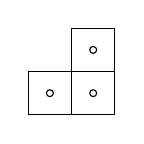
\begin{tikzpicture}[scale=0.55]
 \draw (0,0) rectangle (1,1);
 \draw (1,0) rectangle (2,1);
 \draw (1,1) rectangle (2,2);
 \draw (0.5,0.5) circle (0.08);
 \draw (1.5,0.5) circle (0.08);
 \draw (1.5,1.5) circle (0.08);
\end{tikzpicture}
\end{adjustbox}
$\Gamma(\theta)$ — длина границы.
$U(\theta)$ — число соседей (пар соседей).
Распред. Гиббса
\begin{gather*}
 p(\theta)=
 \frac{\exp\{U(\theta)/T\}}
 {\displaystyle\sum_{\theta\in\mathcal{B}(V_\ell,N)}\exp\{U(\theta)/T\}}
 =\frac{\exp\{-\Gamma(\theta)/(2T)\}}
 {\displaystyle\sum_\theta\exp\{-\Gamma(\theta)/(2T)\}}.
\end{gather*}
[Под первой суммой:] все распол.
\begin{gather*}
 (\text{т. к. }2U(\theta)=2\nu N-\Gamma(\theta)).
\end{gather*}
\underline{Фазовый переход.}
Пусть решётка растёт $\ell\to\infty$,
и пусть $N_\ell\to\infty$.
Предел $V_\ell/N_\ell\to v$ — уд. объём.
Оказ., что
\begin{gather*}
 \frac1N\log\sum_\theta\exp\{U(\theta)/T\}\longrightarrow f(v,T).
\end{gather*}
\Unclear{GELFAND-P000008}{name-van-hove}{Под пределом имя читается «Ван Хов» или «Ванхов»; середина и конец густо переписаны.}
$(v,T)$ наз. точкой фаз. перехода, если
\begin{gather*}
 \frac{\partial f(v,T)}{\partial v}=0
 \quad\text{в нек. окр. при }T=\mathrm{const}.
\end{gather*}
\Unclear{GELFAND-P000008}{temperature-relation}{Между $T$ и const знак похож на $=$ или $\ne$; кандидат $=$ сохранён, чтение не утверждается.}
\Incomplete{GELFAND-P000008}{margin-left}{На самом левом краю виден узкий обрезанный столбик рукописных окончаний соседнего текста; непрерывные слова восстановить нельзя.}

\SourcePage{GELFAND-P000009}{5}
(Т. к. ф-я линейна, a priori она выпукла.)
\begin{gather*}
 Q(T)=\frac{S_\nu e(1-e^{-1/(2T)})}
 {3(1+e^{-\nu/T})}
 \sum_{k=2\nu}^{\infty}3\exp\{-1/(2T)\}^{k}
 k^{\frac\nu{\nu-1}}.
\end{gather*}
[После первого равенства зачёркнутый фрагмент:]
\Unclear{GELFAND-P000009}{q-formula}{Зачёркнутый знак после $=$ не читается. В числителе множитель после $S_\nu$ похож на $e$; верхний предел суммы похож на $\infty$ или двойной штрих. Степень $k$ может относиться также к множителю $3$, но на скане видна у закрывающей фигурной скобки. Варианты не заменены стандартной формулой.}
$S_\nu$ — объём $\nu$-мерн. сф. с $1$ пов.
\begin{gather*}
 S_2=\frac1{4\pi},\qquad S_3=\frac1{C\sqrt\pi}.
\end{gather*}
\Unclear{GELFAND-P000009}{sphere-constant}{Первый множитель знаменателя $S_3$ похож на $C$, $c$ или $6$; запись $C$ — только кандидат.}
Если
\begin{gather*}
 Q(T)<\frac1v<1-Q(T),
\end{gather*}
то имеет место фазовый переход.
\begin{adjustbox}{max width=\linewidth}
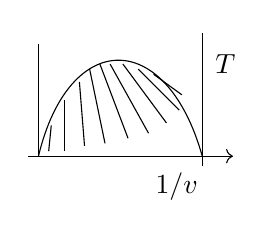
\begin{tikzpicture}[scale=0.65]
 \draw (-0.2,0)--(3.2,0);
 \draw[->] (3.2,0)--(3.8,0);
 \draw (0,0)--(0,2.2);
 \draw (3.2,-0.2)--(3.2,2.4);
 \draw (0,0).. controls (0.6,2.5) and (2.5,2.5)..(3.2,0);
 \draw (0.2,0.1)--(0.25,0.6);
 \draw (0.5,0.1)--(0.5,1.1);
 \draw (0.9,0.2)--(0.8,1.45);
 \draw (1.3,0.25)--(1,1.7);
 \draw (1.75,0.35)--(1.2,1.8);
 \draw (2.15,0.45)--(1.4,1.8);
 \draw (2.5,0.65)--(1.65,1.8);
 \draw (2.75,0.9)--(1.95,1.7);
 \draw (2.8,1.2)--(2.25,1.6);
 \node at (3.65,1.8) {$T$};
 \node at (2.7,-0.6) {$1/v$};
\end{tikzpicture}
\end{adjustbox}
[Разделительная черта.]

$S$ — подкуб. $S_\ell\subset V_\ell$.
$K_\ell$ — сторона $S_\ell$.
\begin{gather*}
 0<d<\frac{K_\ell}{\ell}<1-d.
\end{gather*}
Ввод. случ. велич.
$\mu(S_\ell)$ — число точек расп. $\theta$, попавших в $S_\ell$.
$\mu_{S_\ell}(\theta)$.
Если
\begin{gather*}
 \mathsf{P}\left\{
 \left|\frac{\mu_{S_\ell}(\theta)}{K_\ell^\nu}-\frac1v\right|
 \right\}>\varepsilon\}\overset{/}{\longrightarrow}0,
 \qquad\varepsilon>0,
\end{gather*}
то есть фаз. переход.
\Unclear{GELFAND-P000009}{probability-brace}{На скане после правой черты видна фигурная скобка перед $>\varepsilon$ и ещё одна после $\varepsilon$. Эта несогласованная запись сохранена; кандидат обычного события — модуль больше $\varepsilon$ внутри одной пары скобок.}
[Под первой дробью:] плотн. в подкубе.
[Под $1/v$:] плотн. во всём кубе.
И близкое условие необходимо.
(Физ. смысл — сосущ. $2$-х фаз.)

\begin{adjustbox}{max width=\linewidth}
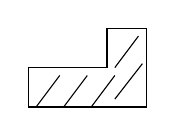
\begin{tikzpicture}[scale=0.5]
 \draw (0,0)--(3,0)--(3,2)--(2,2)--(2,1)--(0,1)--cycle;
 \draw (0.2,0)--(0.8,0.8);
 \draw (0.9,0)--(1.5,0.8);
 \draw (1.6,0)--(2.2,0.8);
 \draw (2.2,0.2)--(2.9,1.1);
 \draw (2.2,1)--(2.8,1.8);
\end{tikzpicture}
\end{adjustbox}
Граница в расп. на компоненты —
— но связь через уголки ($\nu=2$) и ребро ($\nu=3$)
не учитывается.
\begin{gather*}
 \Gamma(\theta)=\sum_i\Gamma_i(\theta).
\end{gather*}
$\Gamma_i(\theta)$ — дл. или площ. компон. границы.
\underline{Определение.} Выделим спец. расположение.
Зав. от $3$-х чисел $N<\infty$, $D<\infty$, $\delta>0$.
\Unclear{GELFAND-P000009}{finite-parameter}{Первая буква похожа на $N$, но допускает $M$; увеличенный фрагмент не снимает различия. Она не согласована автоматически с верхним пределом суммы следующего кадра.}
Циклы занумер. по убыв. длин
\begin{gather*}
 \Gamma_1(\theta)\ge\Gamma_2(\theta)\ge\cdots .
\end{gather*}

\SourcePage{GELFAND-P000010}{unlabelled}
Усл.
\begin{gather*}
 1)\quad\sum_{i=1}^{M}\Gamma_i(\theta)\le D\ell^{\nu-1}.
\end{gather*}
(Порядок пов. большого куба.)
\begin{gather*}
 2)\quad\sum_{i=M+1}^{\infty}
 \bigl(\Gamma_i(\theta)\bigr)^{\frac\nu{\nu-1}}
 \le\frac{\min(N_\ell,V_\ell-N_\ell)}{S_\nu}(1-\delta).
\end{gather*}
\Unclear{GELFAND-P000010}{small-cycles-sign}{Знак неравенства перед дробью густо переписан; кандидаты $\le$ и $<$. Первый параметр верхнего предела первой суммы похож на $M$ или $N$.}
\begin{gather*}
 S_\nu\bigl(\Gamma_i(\theta)\bigr)^{\frac\nu{\nu-1}}
\end{gather*}
Площ. круга с длиной $\Gamma_i$.
Max объём имеет шар, это оц. сверху для объ. об. внутри циклов.
(Он $<$ чем нужно, чтобы помест. все занятые точки.)
([Слово зачёркнуто; сверху вставлено:] объём.
Внутри мелких циклов $<$ заштрих. площ.
и белая площадь.)
\Unclear{GELFAND-P000010}{small-volume-cancellation}{Слово под вставленным «объём» густо зачёркнуто и не читается. «Площ.» в двух строках оставлено как на скане, без замены на объём.}

\SourceFigure{GELFAND-P000010}{diagram-nested-cycles}{Три примерно концентрических контура; внешнее кольцо густо заштриховано, средняя и внутренняя области содержат отдельные штрихи. Точное число контуров и тип отдельных отметок не установлены.}
Нельзя загнать туда ни все точки, ни все пустые места.
Пример расп., когда не вып.
\SourceFigure{GELFAND-P000010}{diagram-phase-mixture}{Прямоугольник разделён почти горизонтальной кривой: сверху три маленькие округлые области, снизу штриховка и несколько округлых незаштрихованных областей. Точные границы и число нижних областей не уверены.}
Это фаз. переход.
Все св. к $2$-м леммам.

$1)$ $\exists M,D,\delta$, что
вер. вып. условий $\longrightarrow1$,
если вып. сформ. условие.
[Под параметрами:] ни от кого не зависят.
\Unclear{GELFAND-P000010}{theorem-condition}{В строке после «если вып.» слово выглядит «сформ.» или «строгое»; не дополнено по смыслу.}

$2)$ \underline{Лемма $2$.}
Если почти все расп. особые, то фаз. переход.
\underline{Идея док. леммы $2$.}
$G$ — объ., об. внутри мал. циклов.
\begin{gather*}
 G\le N_\ell(1-\delta),\qquad
 \frac{G}{V_\ell}\le\frac1v(1-\delta).
\end{gather*}
\SourceFigure{GELFAND-P000010}{diagram-grid}{Справа решётка из вертикальных и горизонтальных линий, в одной центральной клетке жирный квадрат; подпись «Разбили на подкубы». Размер решётки, число клеток и выделенная клетка не читаются точно.}
Сущ. подкуб $S_\ell$:
\begin{gather*}
 \frac{G\cap S_\ell}{V_\ell}\le\frac1v(1-\delta).
\end{gather*}
\Unclear{GELFAND-P000010}{last-fraction}{В числителе перед $\cap S_\ell$ густой знак похож на $G$, в знаменателе явно похоже на $V_\ell$. Сохранён кандидат; мера пересечения и объём подкуба не подставлены по смыслу.}
\SourcePage{GELFAND-P000011}{6}
Пусть все большие циклы \Unclear{GELFAND-P000011}{top-line}{со / $\infty$ окружают. [двухпетлевой знак перед глаголом неуверен]}.

2 случая.
\SourceFigure{GELFAND-P000011}{diagram-01}{Два маленьких прямоугольника: в левом четыре закрашенных кружка; в правом четыре круглых знака, три с видимым светлым центром, нижний правый темнее и плотнее обведён. Внутри правого прямоугольника дополнительные мелкие, местами дугообразные штрихи. Их значение и точные направления не установлены.}

\underline{Лемма.} \Unclear{GELFAND-P000011}{upper-middle}{Непрс. [неуверенное сокращение]} границу из $k$ [зачёркнуто: \Unclear{GELFAND-P000011}{upper-right-cancellation}{точк. [чтение зачёркнутого неуверенно]}; сверху/ниже вписано: звеньев] $\leq 3^k$.

Выигрыш $3$, проиг.
\SourceFigure{GELFAND-P000011}{diagram-02}{Под словами о выигрыше и проигрыше нарисованы горизонтальная линия с короткими крайними штрихами и вертикальный отрезок вниз; это исходная схема без уверенно прочитанных подписей.}
\begin{equation*}
\exp\left\{-\frac{1}{2T}\right\},\qquad
\left(3\exp\left\{-\frac{1}{2T}\right\}\right)^k.
\end{equation*}

\underline{Зад.} (нереш.)
Пусть $N$ велико. Повор. с вер. $\frac13$, но запрещ. [зачёркнуто: \Unclear{GELFAND-P000011}{middle-cancellation-01}{не [неуверенный кандидат короткого слова]}] возвращ.
Каково [зачёркнуто: \Unclear{GELFAND-P000011}{middle-cancellation-02}{вер. ... [первое сокращение-кандидат; следующая отменённая запись не читается]}] мат. ожид. расстояния, на к-рое он уйдёт за $N$ шагов.

(Если разреш. возвращ., то $\sim\sqrt n$.)
Если разреш. возвр., то
\Unclear{GELFAND-P000011}{middle-bound}{$(\geq2{,}6^n\ \text{но}\ <2{,}8^n,\ \text{гипотеза}\ e^n)$; первый знак также может читаться $>$; дополнительные штрихи неуверенны}.

[Горизонтальный разделитель.]

$28/\mathrm{IX}$ \underline{Сигал.}
Теория ф-й на мн. реш. релятив. дифф. ур-я.
[На левом поле: Все они запис. так.]
\begin{equation*}
u'=Au+K(u)\qquad(A)\qquad u(t),\quad -\infty<t<+\infty,
\end{equation*}
\begin{equation*}
A=-A^*,\qquad u\in L^2,\qquad u(t)\in H.
\end{equation*}
$K$ --- зад. нелин. оператор.
В $\int$ форме
\begin{equation*}
u(t)=e^{A(t-t_0)}u(t_0)+\int_{t_0}^{t}e^{A(t-s)}K(u(s))\,ds\qquad(B).
\end{equation*}
Когда $K\in C^1$, т. е. $\partial_uK=K_u$ сущ. по Фреше и непр., то каждое реш. (B) есть реш. A (если $u(t)$ из обл. опр. A).

[Горизонтальный разделитель.]

Пусть (B) им. реш. в целом $\forall$ нач. данным в $t_0$ ($u_0$).
(И $K\in C^1$.)
В квант. мех.
\begin{equation*}
\square\varphi=f(\varphi)
\end{equation*}
[Под знаком $\square$: даламбертиан.]
\begin{equation*}
u(t)=[\varphi(\cdot,t),\dot\varphi(\cdot,t)],\qquad
\varphi=\varphi(\vec x,t).
\end{equation*}
$K$ --- нелин. опер. \Unclear{GELFAND-P000011}{bottom-line}{Немыц. / Намыц. [последнее сокращение неуверенно]}.

\SourcePage{GELFAND-P000012}{unlabelled}
\begin{equation*}
\|[\varphi,\omega]\|\qquad
\square\varphi=m^2\varphi+f(\varphi)
\end{equation*}
[Под формулой: Более кр. форма.]
\begin{equation*}
B=\sqrt{m^2I-\Delta},\qquad
\|[\varphi,\omega]\|=\|B\varphi\|_{L^2}^{2}+\|\omega\|_{L^2}^{2}.
\end{equation*}
\Unclear{GELFAND-P000012}{upper-norm}{В левой части последней формулы над нормой квадрат не виден; правая часть содержит квадраты. Запись сохранена без математического исправления.}
$A$ зад. матрицей 2-го порядка
\begin{equation*}
\begin{pmatrix}0&I\\-B^2&0\end{pmatrix}.
\end{equation*}
Он не самосопр., но в этой норме самосопр.
\Unclear{GELFAND-P000012}{upper-selfadjoint}{Слово «самосопр.» прочитано так в обоих местах; возможное сокращение и согласование с предыдущей записью $A=-A^*$ требуют сверки.}
Любое ур-е релятив. физ. запиш. так.

$M$ --- совок. всех решений.
\begin{equation*}
M=[u(\cdot);\ (**)\ \text{удовл.}]
\end{equation*}
[Справа/под формулой: от $t$; \Unclear{GELFAND-P000012}{upper-right-note}{различные B. [неуверенное чтение подчёркнутой пометы]}]
Пусть теперь $K\in C^\infty$.
$M$ --- Банахово многообр. (у люб. точки есть окр., гомеом. бан. [зачёркнуто: \Unclear{GELFAND-P000012}{middle-cancellation}{неразборчивое слово}] пр-ву, переход --- $C^\infty$ (по Фреше) ф-и).
\begin{equation*}
S_t:M\longrightarrow H,\qquad u(\cdot)\longmapsto u(t).
\end{equation*}
[Справа: оператор. \Unclear{GELFAND-P000012}{middle-right-note}{$\text{мн. реш.}\longrightarrow H$ / $\text{им. реш.}\longrightarrow H$ [первое сокращение неуверенно; конечная стрелка и $H$ видны]}]
\underline{Теорема.} Сущ. единственная $C^\infty$-многообразная структура, что отобр. $S_t$ --- $C^\infty$-изоморфизм.
$u(t,u_0)$ зависит от $u_0$ $C^\infty$-обр.

Истин. многообр.
Есть кас. пр-во $T_{u(\cdot)}$.
Кас. отобр.
\begin{equation*}
dS_t:T_{u(\cdot)}\longrightarrow T_{u(t)}.
\end{equation*}
Кон. $\forall$ точки изом. самому пр-ву.
\begin{equation*}
\lambda\in T_{u(\cdot)},\qquad dS_t(\lambda)=v(t)\in H.
\end{equation*}
Получ. --- каждому кас. вектору соотв. ф-я.
[Подчёркнуто и зачёркнуто: Лемма.]
Обозн. $v(t)$ (не знач. $v$ в т. $t$), ур. вар. ур-е 1-го пор.
\begin{equation*}
v'=Av+K_{u(\cdot)}.
\end{equation*}
\Unclear{GELFAND-P000012}{lower-variation}{После $K_{u(\cdot)}$ отдельный множитель $v$ на этой строке не виден; запись оставлена как в источнике.}
Реш. этого ур-я происх. из кас. вект. $\lambda$ и наоборот.

1) Канонич. дифф. форма на $M$.

2) Скобки Пуассона (анал. с конечномерн. случаем).

\SourcePage{GELFAND-P000013}{7}
3) Вект. поля в $M$. В их терм. будут \Unclear{GELFAND-P000013}{top-line}{зд. [последнее сокращение неуверенно]}.

4) Канонич. коммут. соотн.

5) Будет дано предст. и явное опр. опер.

$5/\mathrm X$. \underline{Сигал.}
I. Ренормализ. ур-е поля.
1) Вывод. 2) Сущ. и ед.

II. Опред. матрицы рассеяния $S$.
A. Классич. $S$-оп.
B. Распр. обобщ. вер. распред. в нелин. сл.

III. Обсужд. вопр. интерпр. с теор. частиц.

[Горизонтальный разделитель.]

Рассм. ур-е
\begin{equation*}
\square\widetilde\varphi=m^2\widetilde\varphi+\widetilde\varphi^3,
\end{equation*}
\begin{equation*}
[\widetilde\varphi(\vec x,t),\widetilde\varphi(\vec x',t)]
=0=[\dot{\widetilde\varphi}(\vec x,t),\dot{\widetilde\varphi}(\vec x',t)].
\end{equation*}
\Unclear{GELFAND-P000013}{middle-commutator}{Кандидаты исходной строки: $[\widetilde\varphi(x),\widetilde\varphi(x')]=i\delta'(x-x')$ / $[\widetilde\varphi(x),\dot{\widetilde\varphi}(x')]=i\delta(x-x')$. Точка над второй буквой, вид дополнительного штриха после $\delta$ и точное положение аргументов не вполне различимы.}

\underline{Loran Schwartz.}
Есть 2 типа мер: меры Радона и просто меры [над последним словом вставлено: абстр.].
Пока огранич. $+$ меры.
\underline{Абстр. мера} на мн-ве $X$, $F$ --- $\sigma$-алгебра.
$\mu$ --- мера. $\mu$ --- $\sigma$-адд. по $F$.

[Горизонтальная линия.]

Когда уже зад. мера, то можно рассм. на $\mu$-изм. мн-ва, $F_\mu$ на $X$ и интегр. измеримые ф-и.
\begin{equation*}
f:X\longrightarrow F,\qquad \int_Xf(x)\,d\mu(x).
\end{equation*}
[Справа: знач. в бан. пр-ве; $F$ --- Бан. пр-во.]

[Горизонтальная линия.]

\underline{Радон. мера.} $X$ --- произвол. лок. компактное.
$C(X)$ --- непр. ф-и с комп. носителями с топ. инд. предела,
и пусть $C'(X)$ сопр. пр-во.
Его элем. --- мера на $X$.

\SourcePage{GELFAND-P000014}{unlabelled}
$\mu$ --- полож., если $\mu(\varphi)\geq0$ при $\varphi\geq0$.
Мера ограничена, если
\begin{equation*}
|\mu(\varphi)|\leq C\max|\varphi|.
\end{equation*}
2-е опрд. --- огранич. полож. Рад. мера.
С ней делается тоже Леб. расширение.
И $\int$ тоже сущ. (знач. в бан. пр-ве).

$\sigma$-поле, постр. по Рад. мере, зависит от $\mu$, но сущ. не завис. от $\mu$ (существ.) --- поле борел. мн-в
(\Unclear{GELFAND-P000014}{upper-borel-note}{min сод. замкн. и откр. [начало скобочной пометы неуверенно]}).

[Горизонтальный разделитель.]

Причина предпочтения радоновых мер различным мат.?
Радон. меры сущ. только на лок.-комп. пр-вах (огранич. теор. вер.).
Но [зачёркнуто: \Unclear{GELFAND-P000014}{middle-cancellation-01}{два коротких неразборчивых слова}] Рад. меры удобнее.
\Unclear{GELFAND-P000014}{middle-uniqueness}{Для правых мер есть разлож. / различ. единицы (если [зачёркнутое начало] мера $=0$ на сист. окр., то она вообще ноль). [Первое определение мер и сокращение перед «единицы» неуверенны.]}
Есть 5--15 теор., верных для Рад. мер (только).

\begin{equation*}
X\overset f\longrightarrow Y
\end{equation*}
[Под стрелкой: топ. пр-ва.]
[Зачёркнуто: \Unclear{GELFAND-P000014}{middle-cancellation-02}{короткое слово перед «Выделим»}.]
Выделим на $X$ и на $Y$ Борелевское поле и абстр. меру $\mu$ на $X$.
И пусть $A\subset Y$.
Тогда есть мера $f(\mu)$ в $Y$:
\begin{equation*}
f(\mu)(B)=\mu(f^{-1}(B)).
\end{equation*}
Но если $B$ --- произв. подмн. $A\subset X$, то [зачёркнут одиночный знак]
\begin{equation*}
f(\mu)(A)\qquad \mu(f^{-1}(A)).
\end{equation*}
\Unclear{GELFAND-P000014}{lower-set-names}{В исходной записи чередуются $A$ и $B$ и перед второй парой формул читается $A\subset X$; буквенные обозначения не согласованы редактором.}
Можно пок., что если левая часть им. смысл, то правая тоже и они равны, но обратное неверно.
[Зачёркнуто: \Unclear{GELFAND-P000014}{lower-cancellation}{неразборчивое начало строки}.]
\begin{equation*}
A\ \text{---}\ f(\mu)\text{-изм.}\ \Longrightarrow\ f^{-1}(A)\ \mu\text{-изм.}
\end{equation*}
Если $\mu$ --- мера Радона, то эквивалентность.

\underline{Пример (противореч.)}
\begin{equation*}
X\subseteq Y=[0,1]
\end{equation*}
так, что $X$ --- неизмеримое по Лебегу мн-во,
$Y\setminus X$ имеет внутр. меру $0$ (или внешн. мера $X=1$).
Подмн. $X$ --- борелево $\Longleftrightarrow$ оно пересеч. с бор. мн. $Y$.
$\mu$ --- абстр. мера.

\SourcePage{GELFAND-P000015}{8}
\underline{Опрд.} $\mu(D)$.
$D\subset X$ --- борел.
\begin{equation*}
D=X\cap E,\qquad E\ \text{--- бор. в }Y,
\end{equation*}
\begin{equation*}
\mu(D)\underset{\mathrm{def}}=dx(E)
\end{equation*}
[Под $dx(E)$: леб. мера.]
\Unclear{GELFAND-P000015}{upper-lebesgue-notation}{В записи $dx(E)$ обе буквы стоят на основной строке; регистр второй буквы не вполне различим: $dx(E)$ / $dX(E)$. Подстрочный индекс не добавлен.}
Мера одна и та же (\Unclear{GELFAND-P000015}{upper-null-note}{отлич. на мн-во вн. меры 0 [скобочная помета неуверенно]}).
Мы опр. абстр. меру на $X$. Образ её
[Следующая строка повторяет: образ её] $dx$.
Возьмём какое-нибудь (не бор.) подмн. $Y\setminus X$.
Оно неизмер., но его прообраз пуст и значит измерим.

Цель докл. --- пок., что не нужна лок.-комп.
Пусть $\mu$ --- мера на $F_B$, тогда $\mu$ есть Рад. мера, если она внутр. комп. рег.
\begin{equation*}
\mu\ \text{Радонова}\ \Longleftrightarrow
\forall B,\ \forall\varepsilon>0\ \exists\text{ комп. }\subset B,\qquad
\mu(b-k)\leq\varepsilon.
\end{equation*}
\Unclear{GELFAND-P000015}{upper-regularity}{В разности читаются строчные $b-k$, хотя перед ней написано $\forall B$. Между «комп.» и $\subset B$ отдельная буква множества не видна; она не подставлена по смыслу.}
[Горизонтальный разделитель.]

\underline{$X$ --- топ. пр-во.}
Найдём меру, обл. всеми св-ми Рад. лок.-комп. мер.
Пусть она опр. (завед.) на бор. мн-вах.
\underline{Опрд. рад. меры, год. не только для лок. комп.}
Пусть $X$ --- вп. регулярно (они могут быть вложены в комп. пр-ва max идеалов).
\begin{equation*}
X,\qquad \widehat X\ \text{--- чех. пополнение }X
\end{equation*}
(max ид. алг. непр. ф-й).
\begin{equation*}
X\overset i\longrightarrow\widehat X.
\end{equation*}
Полная рег. озн., что это гомеом. отобр., а не только инъект. отобр.
Другое опрд. рад. меры над $X$ --- радон. мера на $\widehat X$, при к-рой
\begin{equation*}
\mu(\widehat X\setminus X)=0.
\end{equation*}
Можно пок. эквивалентность.
\underline{В лок. комп.}
\begin{equation*}
\mu\ \mathrm{Rad}\ \Longleftrightarrow\ \forall B\text{ комп.}\ \forall\varepsilon>0\ \exists\text{ комп.}\quad
\mu(B-k)<\varepsilon.
\end{equation*}
\Unclear{GELFAND-P000015}{lower-regularity}{В разности второй знак похож на строчное $k$; первый читается как $B$, но регистр не вполне уверен ($B-k$ / $b-k$). После «комп.» отдельная буква множества и условие включения не видны. Не дополнено по предыдущей формуле.}
Все св-ва Рад. мер выполняются.
Док-во теор. верно в $\widehat X$ и ост. почти трив.
Есть единств. искл. --- [зачёркнуто: \Unclear{GELFAND-P000015}{bottom-cancellation}{св-ва ... бор. ... [видимые фрагменты-кандидаты под горизонтальной чертой; полная отменённая фраза не читается]}] пр-в.
--- нельзя опр. носит. произв. рад. мер.

\SourcePage{GELFAND-P000016}{unlabelled}
$X\subset K_0$ в комп. пр-во (любое). Тогда сущ. аналогичное опр. Рад. мер.
Мы получим тот же закон.

[Горизонтальный разделитель.]

Сравним с опр. ядерного пр-ва (пр-ва в к-рых 2 опр. тенз. произв. совп.).
\begin{equation*}
a(X)\supset R(X).
\end{equation*}
\Unclear{GELFAND-P000016}{upper-space-symbol}{Первый символ в включении похож на строчное $a$ с крупной петлёй; возможное $A$ или каллиграфическая форма не вполне исключены.}
Радон. пр-во, если $\forall$ абстр. мера на нём --- радонова.

3 св-ва рад. пр-в.
1) Если $X$ рад. и $Y\subset X$, то $Y$ радоново $\Longleftrightarrow$ оно универс. измеримо в $X$
(изм. по отн. ко всем рад. мерам --- напр. Борелевское, суслинское и аналитич.).

Важн. критерий.
2) Если $X$ --- рад., то оно универс. измеримо, т. е. изм. $\forall$ объемл. пр-ву и $\forall$ мере.
\Unclear{GELFAND-P000016}{middle-universal}{Сокращение после «изм. ∀» читается как «объемл.» / «объем.»; окончание и наличие надстрочного знака не вполне различимы. Не раскрыто до полного слова.}
Теор. вер. --- всегда опр. вер.

3) Пример широк. класса рад.-пр-в.
Распределения, непр. ф-и и т. д.?
Пусть $E$ --- Т. Л. К. --- сепарабельное пр-во Фреше или их счётный инд. предел.
$F$ --- такое же.
Тогда $\operatorname{Hom}(E,F)$ такие же (снабж. любой топ. между поточ. и комп. сход.).
В частности, двойств. пр-во, само пр-во ($R\longrightarrow E$).
Все пр-ва обобщ., $C^\infty$ ф-й.
И опер. $\mathcal L(S,S)$ тоже радоново пр-во.
\Unclear{GELFAND-P000016}{lower-operator-space}{Над/рядом с закрывающей скобкой имеется короткая помета «ф-и». Отдельный штрих после $\mathcal L(S,S)$ не отделяется уверенно от пометы и скобки; кандидат $\mathcal L(S,S)'$ остаётся неуверенным.}

\underline{Прилож.} Рассм. стох. процесс, зад. как вер. на пр-ве всех ф-й с простой сходим. (поточ.) (мера в этом пр-ве).
Возьмём подпр-во непр. ф-й. Оно измер. в $R^R$.

\SourcePage{GELFAND-P000017}{9}
И значит, вероятность ф-и быть непр. всегда сущ.
Пусть она равна $1$. Тогда есть вер. распр. на этом подпр. и она может быть опр. как просто рад. мера на $C$.
Она соср. на сч. числе комп. мн-в (равностеп. непр.).
Если вер. ф-и быть непр. $1$, то с вер. $1$ все эти ф-и им. общ. модуль непр.
Это верно $\forall$ стох. процесса ($\exists$ общ. mod непр. с вер. $1$).

[Большая незаписанная область; на границе в середине кадра видны отдельные небольшие горизонтальные/дугообразные штрихи.]

$12/\mathrm X$.
\underline{Гиндикин.}
\underline{Вейль.} $G$ --- полупр. гр. Ли, что среди вещ. комп. нет матр. 2-го пор.
\Unclear{GELFAND-P000017}{middle-group-hypothesis}{Сокращения «вещ. комп.» и «матр. 2-го пор.» оставлены по видимой строке, без подстановки теоретической формулировки.}
$\Gamma$ --- дискр. подгруппа, $G/\Gamma$ компактно.
Рассм. деформации $\Gamma$: $\gamma(t)$, $\forall t$ дискр. гр. $\Gamma^{(t)}$.
Трив. способ при пом. внутр. автом.
\begin{equation*}
g(t)\gamma g(t)^{-1}.
\end{equation*}
Факторгр. одна и та же.
При этих усл. всякие деформ. тривиальны.
Дост. док., что
\begin{equation*}
H^1(\Gamma,\mathfrak g)=0.
\end{equation*}
$\mathfrak g$ --- алгебра Ли, на ней предст. $\Gamma$.
Если $\Gamma$ не дискр., то теор. Вейля имеет место, хотя $H^1(\Gamma,\mathfrak g)\ne0$.
\Unclear{GELFAND-P000017}{lower-nondiscrete}{В условии читается «не дискр.»; возможная исходная неточность или сокращение не исправлены.}
Есть представл. $\rho(\gamma)$ в $V^d$. Тогда разм.
\begin{equation*}
p=(2g-2)d+i+i'.
\end{equation*}

\SourcePage{GELFAND-P000018}{unlabelled}
\underline{Лоран Шварц.}
\begin{equation*}
E\ \text{---}\ \mathrm{TVS\ LCH\ QC}.
\end{equation*}
[От $H$ в сокращении проведена помета: хаусдорфова.]
Лок. вып. топ. вект. пр-во, почти полное (всякое замкн. огр. мн-во полное).
$\mathcal H$ --- гильб. подпр-во $E$.
\begin{equation*}
\mathcal H\subset E.
\end{equation*}
[Под включением: отобр. непр.; справа: в $\mathcal H$ гильб. метрика.]
Гильб. топология не совпа., а сильнее топ. в $E$.
\underline{Пример.}
\Unclear{GELFAND-P000018}{upper-example}{Запись включения: $L^2\subset\mathcal D^1$ / $L^2\subset\mathcal D'$; толстый знак справа над $\mathcal D$ похож и на $1$, и на штрих.}
Ещё прим. --- пр-во констант:
\begin{equation*}
(\alpha\mid\beta)=\alpha\overline\beta.
\end{equation*}
\begin{equation*}
\mathcal H\in\mathrm{Hilb}(E)\ \text{--- все гильб. подпр-ва}.
\end{equation*}
[На левом поле повторено: $\mathrm{Hilb}(E)$, со стрелкой к следующему заголовку.]
Абстрактная конич. структура.
Надо определить слож., умн. на $+$ числа и упорядочить.
\begin{equation*}
\mathcal H\in\mathrm{Hilb}(E),\quad \lambda\geq0,\quad \lambda\mathcal H,\quad
\mathcal H_1+\mathcal H_2,\qquad \mathcal H_1\leq\mathcal H_2.
\end{equation*}
При $\lambda=0$, $\lambda\mathcal H$ --- 0-е подпр-во.
При $\lambda\ne0$, $\lambda\mathcal H$ есть то же пр-во со скал. произв.
\begin{equation*}
(h\mid k)_{\lambda\mathcal H}=\frac1\lambda(h\mid k)_{\mathcal H}.
\end{equation*}
$\mathcal H_1+\mathcal H_2$.
Если 0-е пересеч., то прямое.
\begin{equation*}
\|h\|_{\mathcal H_1+\mathcal H_2}
=\inf\left(\|h_1\|_{\mathcal H_1}^2+\|h_2\|_{\mathcal H_2}^2\right),\qquad h=h_1+h_2.
\end{equation*}
[Под формулой: по всевозм. предст.]
\Unclear{GELFAND-P000018}{bottom-norm}{В левой части формулы нормы не виден квадрат, тогда как обе правые нормы возводятся в квадрат. Запись не исправлена.}

\SourcePage{GELFAND-P000019}{10}
\begin{equation*}
\mathcal H_1\oplus\mathcal H_2.
\end{equation*}
Прям. $\Sigma$ как абстр. гильб. пр-в.
\begin{equation*}
(h_1,h_2)\longmapsto h_1+h_2.
\end{equation*}
\SourceFigure{GELFAND-P000019}{diagram-01}{Треугольная схема: сверху слева $H_1\oplus H_2$, сверху справа $E$, снизу фактор $H\oplus H/\mathrm{Ker}$. Горизонтальная стрелка идёт слева направо в $E$, диагональная вниз от прямой суммы к фактору, другая диагональная вверх от фактора к $E$. Индексы у букв в нижней вершине читаются неуверенно. Справа: «Получ. инъект. отобр.»}
Inf --- это как раз опр. нормы в факторпр-ве.
Но факторпр-во гильб. пр-ва само гильбертово.
Итак, это гильбертова норма.
Пусть
\begin{equation*}
H_1\subset H_2\subset E,
\end{equation*}
тогда говорим, что $H_1\leq H_2$.
[Под первым включением стрелка $i$: оператор с нормой $\leq1$.]
\begin{equation*}
\|h\|_{H_1}\geq\|h\|_{H_2}>0.
\end{equation*}
Легко пров. все св-ва:
\begin{equation*}
(\lambda\mu)H=\lambda(\mu H),\qquad
(\lambda+\mu)H=\lambda H+\mu H.
\end{equation*}
И все остальные.
\begin{equation*}
\mathcal H_1+\mathcal H_2\geq\mathcal H_1,\qquad
\lambda\mathcal H\geq\mathcal H\ \Longleftrightarrow\ \lambda\geq1.
\end{equation*}
[Справа от первого неравенства и под второй строкой густо зачёркнуты записи:
\Unclear{GELFAND-P000019}{lower-cancellations}{исходные буквы и знаки под густой штриховкой не читаются}.]
Это аксиом. \underline{выпуклого} конуса.
Сущ. необх. и дост. усл. реализации абстр. кон. структур. в
\Unclear{GELFAND-P000019}{bottom-realization}{евкл. / свкл. пр-ве [начальная буква сокращения неуверенна]}.

\SourcePage{GELFAND-P000020}{unlabelled}
[Первое слово заголовка зачёркнуто: Строгий; сверху вписано: строго выпук.]
абстр. конус:
\begin{equation*}
h\geq h_1\ \Longleftrightarrow\ \exists h_2\text{ единств. (!), что }h=h_1+h_2.
\end{equation*}
Будет док., что конус гильб. подпр-в можно вложить в лин. пр-во,
в частности, вып. это усл.
Надо док., что если $H_1\leq H$, то сущ. единств. $H_2$, что $H=H_1+H_2$.
Вместо этого будет построен конус в лин. пр-ве, к-рому этот изоморфен.
\begin{equation*}
E\ \text{--- пр-во ядер},\qquad H\in\mathcal L(E^*,E).
\end{equation*}
$\mathcal L$ --- пр-во лин. опер. из антидвойств. пр-ва
(антилинейн. [зачёркнуто: \Unclear{GELFAND-P000020}{middle-cancellation}{неразборчивое короткое слово}] ф-лов) в $E$, в слабой топологии в $E$.
По опр.
\begin{equation*}
H\geq0\ \underset{\mathrm{def}}\Longleftrightarrow
\forall e^*\in E^*,\qquad (He^*\mid e^*)_{E,E^*}\geq0.
\end{equation*}
\begin{equation*}
e^*\in E^*,\quad f\in E,\qquad
(e^*\mid f)_{E^*,E}=\overline{(f\mid e^*)_{E,E^*}}.
\end{equation*}
\begin{equation*}
\mathcal L^+(E^*,E)\subset\mathcal L(E^*,E).
\end{equation*}
[Под формулой: конус положит. ядер.]
\underline{Прим.} $E$ --- гильб. пр-во,
\Unclear{GELFAND-P000020}{lower-example-symbol}{$\mathcal L^+$ [исправленный/переписанный знак неуверен]} --- полож. эрмитовы операторы.
Это строго выпуклый конус.
Конус $\mathrm{Hilb}$ ему-изоморфен.
Пусть $\mathcal H\in\mathrm{Hilb}(E)$. Надо постр. отв. ему ядро.
\begin{equation*}
e^*\in E^*;\qquad h\longmapsto(h\mid e^*)_{E,E^*}.
\end{equation*}
[Под правой частью: $e^*$ антилин.]
\SourcePage{GELFAND-P000021}{11}
Это непр. лин. ф-л и на самом $H$, т. к. влож. непр., но тогда $\exists He^*\in\mathcal H$ с пом. к-рого запис. это скал. произв.
\begin{gather*}
(h\mid e^*)_{E,E^*}=(h\mid He^*)_{\mathcal H}.
\end{gather*}
Получили отобр. $E^*\longrightarrow\mathcal H\longrightarrow E$.
Легко пров., что это слабо непр. отобр. $E^*$ в $E$.
\begin{gather*}
\mathcal H\overset{c}{\longrightarrow}E\qquad\text{инъект. вложено.}
\end{gather*}
Оно индуц. отображение
\begin{gather*}
E^*\longrightarrow H^*\cong\mathcal H\hookrightarrow E.
\end{gather*}
\Unclear{GELFAND-P000021}{dual-map}{В обозначении двойственного гильбертова пространства написано $H^*$; последняя стрелка совмещена со знаком включения.}
Мы имеем отобр. $E^*\longrightarrow E$, что и требовалось.
Пусть $h=Hf^*$, тогда получим
\begin{gather*}
(Hf^*\mid e^*)_{E,E^*}=(Hf^*\mid He^*)_{\mathcal H},\\
(He^*\mid e^*)\ge0.
\end{gather*}
\begin{gather*}
\operatorname{Hilb}(E)\longrightarrow\mathcal L^*(E^*,E).
\end{gather*}
\Unclear{GELFAND-P000021}{positive-map}{Верхний знак у $\mathcal L$ выглядит как $*$; возможен $+$.}
Надо док., что это изом.
Будет док., что оно вз. однозн. на алг. просто. Топ. затруднения.
Если $H$ --- ядро, отв. $\mathcal H$, то $\forall e^*\in E^*$
\begin{gather*}
He^*\in\mathcal H,\qquad
\mathcal H_0=\{He^*:e^*\in E^*\},\\
\underline{u,v\in\mathcal H_0}\qquad
(u\mid v)_{\mathcal H_0}=(Hf^*\mid e^*)_{E,E^*}
=\overline{(He^*\mid f^*)_{E,E^*}}.
\end{gather*}
\Unclear{GELFAND-P000021}{bottom-pairing}{Связь $u,v$ с $e^*,f^*$ здесь не выписана; над последним скалярным произведением видна черта.}

\SourcePage{GELFAND-P000022}{unlabelled}
\underline{Теор. Макки}: мн-во огранич., если оно слабо ограничено.
Док-ть, что ед. шар слабо ограничен.
\Unclear{GELFAND-P000022}{top-proof}{Сокращение в начале второй строки: Док-ть / Док-ц.}
\underline{Примеры}.
\begin{gather*}
E=\mathcal D',\qquad E^*=\mathcal D,\qquad\mathcal H=L^2.
\end{gather*}
$\mathcal L(\mathcal D;\mathcal D')$ --- пр-во ядер, опер. из $\mathcal D$ в $\mathcal D'$.
$\mathcal H=L^2$ определ. ест. отображ. $\mathcal D\longrightarrow\mathcal D'$.
Если $\mathcal H$ произв., то получ. произв. положит. опер., но по теор. о ядре он зад. обобщ. ф-ей 2-х пер.
\begin{gather*}
H_{x,\xi}\in\mathcal D'(R^n\times R^n),\qquad
\iint H_{x,\xi}\varphi(x)\overline{\varphi(\xi)}\,dx\,d\xi\ge0.
\end{gather*}
Есть соотв. между гильб. подпр. $\mathcal D'$ и такими ядрами.
$\mathcal H^1$ --- пр-во ф-й, [зачёркнуто: \Unclear{GELFAND-P000022}{sobolev-cancel}{неразборчивое слово перед $L^2$}] $L^2$ с 1-ми произв.
\begin{gather*}
(f\mid g)_{\mathcal H}=\int\left(\lambda f\bar g+\sum\frac{\partial f}{\partial x_i}\frac{\partial\bar g}{\partial x_i}\right)dx.
\end{gather*}
$\lambda>0$ \Unclear{GELFAND-P000022}{lambda-note}{неважно / написано; на них / на нём.}
Двойств. $\mathcal H^{-1}$.
$\mathcal H^1$ отвеч. ядро $-\Delta+\lambda$.
\Unclear{GELFAND-P000022}{sobolev-kernel}{Написано $\mathcal H^1$ отвеч. ядро $-\Delta+\lambda$; возможная связь с предыдущим $\mathcal H^{-1}$ не пояснена.}
Если рассм. ф-и на области $\Omega\subset R^n$, то тоже их примеры:
\begin{gather*}
\mathcal H^{-1},\quad\mathcal H^1,\quad\mathcal H^1_0\quad\text{замык. }\mathcal D_0.
\end{gather*}
\Unclear{GELFAND-P000022}{test-space}{Последний знак выглядит как $\mathcal D_0$, возможны $\mathcal D$ или $\mathcal D_\Omega$.}
Можно получить теор. сущ. реш. как обобщ. ф-й.

\SourcePage{GELFAND-P000023}{12}
\Unclear{GELFAND-P000023}{top-edge}{У верхней границы два обрезанных наклонных штриха, значение неясно.}
Рез. \underline{Кушниренко} об энтропии дин. систем.
\underline{Арнольд}. [Зачёркнуто: \Unclear{GELFAND-P000023}{heading-cancel}{Это / что.}] Энтропия --- скорость, с к-рой забывает нач. данные.
\begin{gather*}
0\qquad h\qquad+\infty.
\end{gather*}
Под $0$: с медл. перемешив. Под $+\infty$: сильное перемешивание.
энтр. для абстр. дин. сист. (сохр. меру $T$ преобр.).
$M^n$ --- гл. многообр. $M^n$ --- компактное.
$T$ --- гладкое, мера $M=1$ и зад. рим. метрикой.
Тогда энтр. всегда конечна и оценив. через лок. св-ва преобр.
\begin{gather*}
h(T)\le n\log\lambda.
\end{gather*}
$n$ --- разм. пр-ва. $\lambda$ --- коэфф. растяж. $(n-1)$-мерн. площади.
Оценка достигается.
\begin{gather*}
\lambda=\sup\frac{dS(Tx)}{dS(x)}.
\end{gather*}
Док. из изоперим. неравенства.
$h$ оцен. через площадь.
Энтр. разбиения $h(\xi)=-\sum p_i\log p_i$.
\SourceFigure{GELFAND-P000023}{partition-drawing}{Справа окружность с диагональным разделителем сверху слева вниз вправо, ответвлением влево вниз и дугой вправо. Левый нижний отрезок двойной или имеет стрелку; точное чтение штрихов неуверенно.}
Разбиение $T\xi$ и пересечение.
\begin{gather*}
h(T^{n-1}\xi,\ldots,T^2\xi\cdot T\xi\cdot\xi)\qquad n^2\text{ кусков},\\
\text{Кусков }\sim k^n,\\
\lim\frac{h(\ldots)}n=h(\xi).
\end{gather*}
[Перед дробью зачёркнуто $\log$.]
\Unclear{GELFAND-P000023}{join-notation}{Между $T^2\xi$, $T\xi$, $\xi$ стоят точки; рядом написано $n^2$ кусков. Обозначение результата предела выглядит как $h(\xi)$.}
для одинаковых $\sum\frac1k\log k=\log k$.
Энтр. дин. сист. $\sup(h(\xi))=h(T)$ --- Колмогоро-ская.
\Unclear{GELFAND-P000023}{bottom-name}{Последнее слово разбито на строки: Колмогоро- / -ская; возможна утрата букв в сокращении.}

\SourcePage{GELFAND-P000024}{unlabelled}
Энтр. разбиения оценив. через площадь границы разбиения. А площадь границ просто складывать!
Для взаимно однозначн. можно поставить вместо $n$ --- $n-1$ и [зачёркнуто: \Unclear{GELFAND-P000024}{boundary-cancel}{неразборчивое слово}] тоже такая оценка.

\underline{19/X}.
[Зачёркнутый заголовок: Лоран Шварц.]
Один физик о предст. алгебр Ли.
\Unclear{GELFAND-P000024}{kostant-reference}{Костант / Констант / Конец.} B. Kostant 93, 53 (1959).
\underline{Повзнер.}
Опред. своб. энергии.
\begin{gather*}
H=p^2+u,\qquad
\frac{-\ln\frac1{N!}\iiint_V^{N}e^{-\beta(H\,+\,\text{[зачёркнуто]})}\,dx}{N}.
\end{gather*}
\Unclear{GELFAND-P000024}{energy-cancel}{После $H$ внутри показателя несколько зачёркнутых знаков; виден $+$ и наложенные штрихи.}
$N$ --- число интегралов.
\Unclear{GELFAND-P000024}{number-word}{Последнее слово после число выглядит как интегралов; возможны интервалов / частиц.}
\begin{gather*}
\frac VN=\mathrm{const},\qquad\beta=\frac1T,\\
\lim_{\substack{N\to\infty\\ V/N=v=\mathrm{const}}}
\frac{-\ln\frac1{N!}\iiint_V e^{-\beta H}\,dx}{N}
\qquad\text{своб. энергия.}
\end{gather*}
\Unclear{GELFAND-P000024}{energy-domain}{У первого тройного интеграла верхний $N$ и нижний $V$; у повторной формулы различим только $V$.}
Энтропия по термодин. ф-лам:
\begin{gather*}
S=-\frac{\partial F}{\partial T},\qquad
\text{давление}\quad p=-\frac{\partial F}{\partial V}.
\end{gather*}
Энтропию можно опред. так:
\begin{gather*}
\frac1N\sum_{i,j=1}^{N}u(x_i,\,-x_j)\le\xi.
\end{gather*}
\Unclear{GELFAND-P000024}{energy-arguments}{Между $x_i$ и $-x_j$ виден штрих, похожий на запятую; возможен только знак разности. Правая буква выглядит как $\xi$.}
Найти все такие $x$.

\SourcePage{GELFAND-P000025}{13}
Взять объём этой обл. в фаз. пр-ве. $P$.
В правом верхнем поле: $x_i\in V$.
\begin{gather*}
\lim_{N\to\infty}\frac{\ln\frac1{N!}P(\xi,V/N)}N
=S(\xi,v)\pm c\ln T.
\end{gather*}
\Unclear{GELFAND-P000025}{entropy-sign}{Перед $c\ln T$ виден крест над отдельной горизонтальной чертой: $\pm$ / $+$.}
$\xi$ --- энергия.
В правом поле: т. к. весь фаз. пр-во по импульсам.
\Unclear{GELFAND-P000025}{entropy-margin}{Весь / всё фаз. пр-во по импульсам.}
$S$ есть выпуклая ф-я от 2-х перем.
О раб. Вигнера (1932 г.) о квант. механике.
Пусть $\Psi(x)$ задаёт вероятности по изв. ф-ле $|\Psi^2(x)|$
и
\begin{gather*}
\widetilde\Psi(p)=\int e^{-ipx/\hbar}\Psi(x)\,dx.
\end{gather*}
\Unclear{GELFAND-P000025}{wigner-power}{В первой строке написано $|\Psi^2(x)|$, тогда как ниже стоит $|\Psi(x)|^2$; степень не переставлена.}
\Unclear{GELFAND-P000025}{fourier-h}{В знаменателе показателя буква $h$ с поперечным штрихом: $\hbar$ / $h$.}
Если
\begin{gather*}
\int P(x,p)\,dp=|\Psi(x)|^2,\qquad
\int P(x,p)\,dx=|\widetilde\Psi(p)|^2,
\end{gather*}
то что такое $P$?
Она стр. в работе Вигнера и отсюда можно перейти от класс. мех. к статист.
\Unclear{GELFAND-P000025}{wigner-word}{Она стр. / она стро.; сокращение перед в работе.}

\underline{Кириллов о работе Тома.}
Elmar Thoma. Math. Zeitschr. 84 (1964).
Если $G$ дискр. некомм. гр., то предст. опис. трудно, но хар. найти можно (положит. непр. ф-и).
\begin{gather*}
\begin{pmatrix}a&b\\0&1\end{pmatrix}.
\end{gather*}
Характ. те же (те же ф-лы как и на вещ., конечн. и $p$-адич. числах).
\Unclear{GELFAND-P000025}{thoma-adjective}{Положит. непр. ф-и: сокращение непр. не раскрыто; возможно непрерывные / неприводимые по контексту.}

\underline{Лоран Шварц.}
$s\in G$ --- группа Ли. $dx$ --- мера Хаара (двустор.).
$\mathcal H$ --- [зачёркнуто: \Unclear{GELFAND-P000025}{space-cancel}{неразборчивое слово}] ТВП.
$U_s$ --- представление в нём.
$a\in\mathcal H$, к-рый беск. дифф. отн. группы; его орбита --- $C^\infty$, как ф-я $s$.
\begin{gather*}
s\longrightarrow A_a(s)=U_sa\in\mathcal H\qquad\text{траектория.}
\end{gather*}
\Unclear{GELFAND-P000025}{orbit-join}{Между $U_s$ и $a$ соединительный штрих, похожий на начало скобки; в тексте записано произведение.}

\SourcePage{GELFAND-P000026}{unlabelled}
$A_a:G\longrightarrow\mathcal H$, к-рая $C^\infty$.
Вместо предст. $U_s$ можно рассм. $U_\mu$ и $U_\varphi$.
\begin{gather*}
U_\mu=\int U_s\,d\mu(s).
\end{gather*}
Траектория
\begin{gather*}
U_sA_a(t)=A_a(st).
\end{gather*}
Если есть такая кривая, то она орбита, т. е.
\begin{gather*}
\mathcal H\supset\mathcal H^m\supset\mathcal H^\infty.
\end{gather*}
Под $\mathcal H^m$: траект. $m$ раз дифф. Под $\mathcal H^\infty$: траект. $C^\infty$.
Можно док., что $\mathcal H^{+\infty}$ плотно в $\mathcal H$ (усреднением).
Определим
\begin{gather*}
\mathcal H^{-\infty}\supset\mathcal H\supset\mathcal H^m\supset\mathcal H^{+\infty}.
\end{gather*}
Точечные обобщ. ф-и.
Будем рассм. $U_sA_a(t)=A_a(st)$ как распределение по Хаар. мере.
\begin{gather*}
U_\varphi A_a(\psi)=A_a(\varphi*\psi).
\end{gather*}
Обобщ. точки пр-ва представления.
\begin{gather*}
A:\mathcal D'(G;\mathcal H),\\
\forall\varphi\in\mathcal D(G),\quad A(\varphi)\in\mathcal H,\\
U_\varphi A(\psi)=A(\varphi*\psi).
\end{gather*}
В правом поле, рядом с двумя вертикальными стрелками вниз: обобщ. точки --- её опр. и доп. облад. св-вом свёртки.
\Unclear{GELFAND-P000026}{definition-note}{Её / их опр.; сокращение доп. / долж. облад. св-вом свёртки.}
В частности обычные точки облад. этими св-ми.
Топ. $\mathcal H^{-\infty}$ [зачёркнуто: \Unclear{GELFAND-P000026}{topology-cancel}{неразборчивое слово}] из $\mathcal D'$. $\mathcal H^{-\infty}$ будет полно.
Группа действ. и в $\mathcal H^{-\infty}$.
Там гр. действ. $C^\infty$.
\begin{gather*}
U_\xi^{-\infty}A=\underbrace{A*\check\xi}_{\xi\text{ --- конечн. носит.}}
\end{gather*}
\Unclear{GELFAND-P000026}{measure-symbol}{Индекс и последний символ напоминают $\xi$ / $S$ / $\zeta$; над последним стоит перевёрнутая шляпка.}
Если $\xi=\delta$, то получ. исх. представление.

\SourcePage{GELFAND-P000027}{14}
В частн., алг. Ли тоже действ. ($\delta'$).
[Горизонтальный пунктир отделяет следующую задачу.]
\underline{Задача}. $\Box X=A$, \underline{ур-е с пост. коэфф.}
Это ур-е разрешимо (Ehrenpreis).
Пусть $A$ --- Лор.-инв. Тогда сущ. Лор.-инв. $X$.
\begin{gather*}
\mathcal D X=A.
\end{gather*}
То же для произв. группы и дифф. опер. --- проблема!
\Unclear{GELFAND-P000027}{general-operator}{В повторной формуле перед $X$ округлая буква $\mathcal D$ / $D$; в первой формуле прямоугольник $\Box$.}
\underline{Решение для группы Лоренца.}
\begin{gather*}
\Box X=A.
\end{gather*}
Надо [зачёркнуто: \Unclear{GELFAND-P000027}{lorentz-cancel}{короткое неразборчивое слово}] изучить Лор.-инв. ф-и.
Рассм. $R^n\setminus0$.
Это $T(x_1^2+\cdots+x_n^2-x_0^2)$ от одной пер.
Все непр. из-за некомпактности (иначе можно усреднить).
Для $X$ ищ. инв. распр. от 1-го пер.
Волн. опер. превр. в опер. от 1-го пер., но с переменными коэфф.
Но для 1-го пер. решается.
Но если есть группа с 2-мя инвар., то получ. вместо ос. в 1-й точке линии особенностей и т. д.
Но наше реш. с выбр. точкой. Как всюду?
Использ. рез., что обобщ. ф-я, инв. всюду, кроме кон., может быть распр. в начало.
Степенной рост вытекает из Лоренц.-инв.
\Unclear{GELFAND-P000027}{extension-text}{В последних строках: выбр. точкой; рез. / реш.; кроме кон.; в начало / в начале. Неясное сокращение не раскрыто.}

\SourcePage{GELFAND-P000028}{unlabelled}
Гр.-Лор. полупростая и пр-во конечно-мерно.
Предст. кон.-мерной полупр. гр. Ли имеет неподв. точку (напр. при однор. 0) (одно из опр. полупр. группы).
\Unclear{GELFAND-P000028}{fixed-point-note}{В скобках: при однор. 0 / при одноп. 0; сокращения сохранены.}
Другая зад.
$G$ --- группа Ли.
Опер. Ли $X$ --- беск. малый сдвиг $Xf(g)$.
Рассм. полином от опер. Ли. Как найти элем. решения? (фунд.) $PE=\delta$.
\begin{gather*}
P(X_1,\ldots,X_n)\qquad\text{полином от операторов Ли.}
\end{gather*}
Для кон. групп это, вероятно, неверно.
На торе элемент. решения нет.
Для тора нет реш. Но у тора есть фунд. группа.
А у группы вращ.
\begin{gather*}
\frac{\partial}{\partial x}-\alpha\frac{\partial}{\partial y}.
\end{gather*}
\Unclear{GELFAND-P000028}{operator-power}{У коэффициента $\alpha$ маленький верхний изгиб: $\alpha$ / $\alpha^2$. У знаков $\partial$ отдельной степени 2 не различается.}
В правом поле: $\alpha$ --- иррац., хорош. аппрокс.
\Unclear{GELFAND-P000028}{alpha-note}{Последние два сокращения в поле: хорош. / хорошо; аппрокс.; без восстановления условия на $\alpha$.}
Вращ. есть тоже всюду мн. сингуляр.
\Unclear{GELFAND-P000028}{rotation-word}{Перед сингуляр. короткое сокращение мн. / им.; слово сингуляр. подтверждено повторным просмотром.}
Нетрив. и для операторов 1-го порядка.
\begin{gather*}
E(P\varphi)=\varphi(0).
\end{gather*}
Предп., что для некомм. группы всё будет в порядке.
Для окружности\ldots
\Unclear{GELFAND-P000028}{noncomm-word}{Некомм. / некомп.; сокращение перед группы.}

\SourcePage{GELFAND-P000029}{15}
\underline{2/XI}. \underline{Кириллов.}
\underline{Elmar Thoma}. 3 работы, предст. счётных некомм. групп дискр.
$G$. Сущ. явн. вид для нек-рых групп $+$ опр. ф-и, пост. на кл. сопр. элем. --- крайние точки мн-ва таких ф-й.
\begin{gather*}
f(g)\quad+\text{ опр., если}\quad
\lVert f(g_i g_j^{-1})\rVert\gg0\quad+\text{ опред.}\\
g_1,\ldots,g_n\quad\text{любой набор эл.}
\end{gather*}
$f(e)=1$ --- выпуклое мн-во $M$.
\begin{gather*}
f(g_1g_2)=f(g_2g_1)\quad\text{(пост. на кл. сопр. элем)},\\
f(g)=f(g_1gg_1^{-1}).
\end{gather*}
[Условия о постоянстве на кл. сопр. элем. выделены прямоугольными штрихами справа и снизу.]
Крайние точки наз. характерами непр. предст.
\Unclear{GELFAND-P000029}{character-adjective}{После характерами написано непр. / нер.; сокращение не раскрыто.}
\underline{Пример}: $g\longrightarrow T(g)$,
$\frac1n\operatorname{Sp}T(g)$ --- пример такой ф-и.
Если предст. неприв., то такие ф-и обр. крайние точки --- легко проверить.
(Этой ф-ей предст. опред. однозначно.)
Есть гр. для к-рых опис. предст. невозможно (по теор.-множ. сообр. --- их много), но характеры существ. и выпис. ф-лами.
\begin{gather*}
\begin{pmatrix}\alpha&\beta\\0&1\end{pmatrix}
\quad\text{группа афф. преобр. прямой},\\
x\longrightarrow\alpha x+\beta,\qquad
\alpha,\beta\quad\underline{\text{рациональны}}.
\end{gather*}
Если $\alpha$ и $\beta\in$ кон. поле ($\operatorname{mod}p$), как найти все следы (неприв. представл.).
\underline{Предст.} --- компл. числа.
Не сделано, если предст. дан. с $\alpha,\beta\in(\operatorname{mod}p)$.
\begin{gather*}
\begin{pmatrix}\alpha&\beta\\0&1\end{pmatrix}
\begin{pmatrix}\gamma&\delta\\0&1\end{pmatrix}
=\begin{pmatrix}\alpha\gamma&\alpha\delta+\beta\\0&1\end{pmatrix}.
\end{gather*}
В правом поле: сделано для рациональных.
Одномерные предст. --- все --- $e^{\alpha\frac{2\pi i}{p}}$.
$(p-1)$ предст., зав. только от $\alpha$ --- характеры мульт. гр.
\Unclear{GELFAND-P000029}{multiplicative-character}{В показателе видны $\alpha\,2\pi i/p$; эта запись оставлена при упоминании мультипликативной группы, без исправления знаменателя или параметра.}
\SourceFigure{GELFAND-P000029}{cancelled-bottom}{В нижнем левом углу зачёркнуты два дробных выражения, горизонтальная стрелка и 0; слева и снизу скобкообразные штрихи. Чтение исходной схемы ненадёжно.}

\SourcePage{GELFAND-P000030}{unlabelled}
\begin{gather*}
\sum k_i^2=p(p-1),\\
\sum'k_i^2=p(p-1)-\underbrace{(p-1)}_{\text{одном.}}=(p-1)^2.
\end{gather*}
В правом поле, отделено двойной вертикальной чертой: гр. кольцо --- прям. сумма матр. колец и как раз $\sum k_i^2$.
\underline{Гипотеза}: ещё предст. порядка $\underline{p-1}$.
\underline{Предст.} --- функтор с неизвестным полем.
Для поля беск. пор. ест. бесконечномерн. $(\alpha,\beta)$.
\Unclear{GELFAND-P000030}{functor-note}{Беск. пор. ест. бесконечномерн.; последняя строка тесно прилегает к следующей матрице, её связь с предыдущим функтор с неизвестным полем не раскрыта.}
\begin{gather*}
\begin{pmatrix}1&\beta\\0&1\end{pmatrix}
\qquad\text{найти огранич. предст. на такой гр.},\\
\begin{pmatrix}1&\beta\\0&1\end{pmatrix}
\begin{pmatrix}1&\beta'\\0&1\end{pmatrix}
=\begin{pmatrix}1&\beta+\beta'\\0&1\end{pmatrix}.
\end{gather*}
Одном. предст. её
\begin{gather*}
\begin{pmatrix}1&\beta\\0&1\end{pmatrix}
\longrightarrow e^{\frac{2\pi ik}{p}\beta}.
\end{gather*}
\begin{gather*}
\begin{pmatrix}1&\beta\\0&1\end{pmatrix}
\quad\text{норм. делитель.}
\end{gather*}
Преобр. с [зачёркнуто короткое слово]
\begin{gather*}
\begin{pmatrix}\alpha&0\\0&1\end{pmatrix}
\begin{pmatrix}1&\beta\\0&1\end{pmatrix}
\begin{pmatrix}\alpha^{-1}&0\\0&1\end{pmatrix}
=\begin{pmatrix}1&\alpha\beta\\0&1\end{pmatrix}.
\end{gather*}
\Unclear{GELFAND-P000030}{conjugation-cancel}{Между с и матрицей небольшой затёртый знак или слово.}
\begin{gather*}
\begin{pmatrix}1&\beta\\0&1\end{pmatrix}\longrightarrow T_\beta,\qquad
T_{\beta_1+\beta_2}=T_{\beta_1}T_\beta.
\end{gather*}
[Зачёркнуто: \Unclear{GELFAND-P000030}{commuting-cancel}{короткое слово перед коммут.}] коммут.
\Unclear{GELFAND-P000030}{product-index}{У последнего $T_\beta$ индекс 2 не различим; не дописан по правилу представления.}
Разл. пр-во на соб. вект. отн. $T_\beta$.
\begin{gather*}
T_\beta e_k=e^{\frac{2\pi ik}{p}\beta}e_k,\\
S_\alpha T_\beta S_\alpha^{-1}=T_{\alpha\beta},\\
T_\beta S_\alpha e_k=e^{\frac{2\pi i}{p}\alpha k\beta}(S_\alpha e_k),\\
S_\alpha e_k=e_{\alpha k}.
\end{gather*}
\Unclear{GELFAND-P000030}{conjugation-eigenvalue}{Написаны и $S_\alpha T_\beta S_\alpha^{-1}=T_{\alpha\beta}$, и множитель $\alpha k\beta$ при $T_\beta S_\alpha e_k$; возможная несовместимость сохранена. Под знаменателем последнего показателя есть зачёркнутые знаки.}
Внизу справа: множ. можно взять равными 1.
\Unclear{GELFAND-P000030}{normalization-note}{Перед можно короткое слово: множ. / норм.; не добавлен невидимый коэффициент к $S_\alpha e_k=e_{\alpha k}$.}
\SourcePage{GELFAND-P000031}{16}
Останется $(p-1)$ вектор. Написано, как действует.
Более красивая реализация.
\begin{equation*}
x\longmapsto\alpha x+\beta.
\end{equation*}
[Справа: афф. прям. над конечн. полем.]
$f(x)$ --- ф-и на ней.
\begin{equation*}
T_gf(x)=f(\alpha x+\beta).
\end{equation*}
Const --- инвар., то это предст. привод.
Будем рассм. ф-и, где
\begin{equation*}
\sum_xf(x)=0\qquad(\int=0).
\end{equation*}
Это $(p-1)$-мерн. предст.
\begin{equation*}
\operatorname{Sp}(T_g)=
\begin{cases}
1&\text{при }\alpha\ne1,\\
0&\text{при }\alpha=1,\ \beta\ne0,\\
p&\text{при }\alpha=1,\ \beta=0.
\end{cases}
\end{equation*}
\Unclear{GELFAND-P000031}{trace-third-condition}{В третьем условии после $\alpha=$ знак похож на $1$, $\alpha$ или $p$; показанное $1$ --- только кандидат.}
[Слева под скобкой отдельно повторено: $\alpha\ne1$. Справа подчёркнуто: неприводимо.]
\begin{equation*}
x=\alpha x+\beta,\qquad x=\frac{\beta}{1-\alpha}.
\end{equation*}
\underline{Надо вычесть} след.
\begin{equation*}
\operatorname{Sp}T_g=
\begin{cases}
0&\alpha\ne1,\\
-1&\alpha=1,\ \beta\ne0,\\
p-1&\alpha=1,\ \beta=0.
\end{cases}
\end{equation*}
\Unclear{GELFAND-P000031}{trace-overwrite}{Перед $1$ во втором условии видны густо переписанные/зачёркнутые черты: прежний знак $\ne$ / $=$ не устанавливается уверенно.}
Как связ. с дин. системами?

Пусть $\alpha$ и $\beta$ --- вещественные.
\begin{equation*}
\beta\longmapsto T_\beta,\qquad
T_{\beta_1+\beta_2}=T_{\beta_1}T_{\beta_2},
\end{equation*}
\begin{equation*}
S_\alpha,\qquad S_{\alpha_1\alpha_2}=S_{\alpha_1}S_{\alpha_2},
\qquad S_\alpha^{-1}T_\beta S_\alpha=T_{\alpha\beta}.
\end{equation*}
[Горизонтальная линия.]
Как их найти?
Их можно привести к диаг. форме (пред. \underline{унит.}).
\begin{equation*}
T_\beta f(\chi)=\chi(\beta)f(\chi).
\end{equation*}
[Справа от формулы зачёркнуто: $\chi(\beta)$.]
Прив. к опер. умн. на ф-ю,
где
\begin{equation*}
\chi(\beta_1+\beta_2)=\chi(\beta_1)\chi(\beta_2).
\end{equation*}
[В правой скобке: \Unclear{GELFAND-P000031}{right-vector-note}{$f(\chi)$ --- вект. ф-я, $\forall\chi$ --- пр-ву [знак/сокращение перед $\chi$ и конец неуверенны]}.]
[На левом поле, повёрнуто: дин. сист. на аддит. группе --- [стрелка к строке] мульт. группа действ. на ней.]
\begin{equation*}
S_\alpha f(\chi)=f_1(\chi),
\end{equation*}
\begin{equation*}
T_\beta f_1(\chi)=T_\beta S_\alpha f(\chi)
=S_\alpha T_{\alpha\beta}f(\chi)
=\chi(\alpha\beta)f_1(\chi).
\end{equation*}
\Unclear{GELFAND-P000031}{bottom-symbol-cancellation}{В последнем равенстве перед $\chi(\alpha\beta)$ густо зачёркнут знак, похожий на $S$ / $S_\alpha$; он не включён в действующее выражение и не восстановлен уверенно. Под отменой и под $\chi(\alpha\beta)$ проведены горизонтальные стрелки.}
[В правом нижнем поле, в ступенчатом обрамлении:]
\Unclear{GELFAND-P000031}{bottom-right-notes}{Кажд. точка --- во всюду пл. мн-во. [Кандидаты первых строк; «пл.» перед «мн-во» не читается вполне уверенно.]}
Эргодичная система. С разными мерами --- разные предст.
\Unclear{GELFAND-P000031}{bottom-haar-note}{Мера Хаара --- непр. пр. [последнее сокращение может читаться «гр.»; запись не раскрыта]}

\SourcePage{GELFAND-P000032}{unlabelled}
\Unclear{GELFAND-P000032}{table-heading}{Перед первой матрицей написан символ, похожий на $\overline\chi_K(\alpha)$; индекс может быть кириллической «к», аргумент может быть $g$. Под ним: норм. хар. [первое сокращение неуверенно].}
\begin{equation*}
\begin{array}{ccc|c}
\begin{pmatrix}\alpha\ne0&\beta\\0&1\end{pmatrix}&0&&0\\[4pt]
1\ \begin{pmatrix}1&\beta\ne0\\0&1\end{pmatrix}&-\dfrac1{p-1}&&0\\[4pt]
1\ \begin{pmatrix}1&0\\0&1\end{pmatrix}&1&&1
\end{array}
\end{equation*}
\Unclear{GELFAND-P000032}{table-first-condition}{В верхней левой записи читается $\alpha\ne0$, хотя по соседней таблице следов можно было бы ожидать $\alpha\ne1$. Видимый $0$ не заменён по смыслу. Отдельные $1$ перед двумя нижними матрицами сохранены как видимые записи.}
[Справа от первого верхнего $0$: Хар. для конечн. групп.]
Если перейти к пред. при $p\longrightarrow\infty$.
[От строки о пределе стрелка вверх к правому нижнему $1$.]
\SourceFigure{GELFAND-P000032}{arrow-left}{Подчёркнутое слово на левом поле похоже на «Одном» / «Одному». От области под ним идёт длинная дугообразная линия с наконечниками к левому слову и вправо под область предела. Значение подписи не установлено; направления и форма сохранены описанием.}
То, что осталось для рац. чисел.

\underline{Лемма.}
$G$, $G_0\subset G$ [под $G_0$: норм. дел.].
$f$ --- пол. опр., $f(e)=1$, пост. на сопр.
$M$ --- мн-во их.
Рассм. $f|_{G_0}$.
Ещё рассм. ф-и, уд. на $G_0$ тем же [зачёркнуто: \Unclear{GELFAND-P000032}{middle-cancellation}{короткая запись перед «усл.»}] усл.
Рассм. $H_{G_0}$ --- их крайние точки.
\Unclear{GELFAND-P000032}{extreme-points-line}{Они совп. с крайними точками исх. гр. [последнее сокращение может быть «сч. гр.»; не раскрыто по смыслу].}
(Для счётных групп.)
Надо посчит., сколько есть сопр. классов и тогда ищ. представляющ.
\Unclear{GELFAND-P000032}{lower-cancellation}{Из + опр. [зачёркнутая запись, похожая на «чего-то»] след., что нет других представл.}
[На левом поле: 2-я раб.]

\underline{Беск. симметр. группа:} подстан. натур. ряда
(движ. лишь конечное число эл. --- для счётности).
Кл. сопр. эл. зад. \underline{циклами}.
[Зачёркнуто короткое слово: \Unclear{GELFAND-P000032}{bottom-cancellation}{знак/слово перед «длины циклов» не читается под штрихами}.]
Длины циклов опр. класс сопр. элементов.
\begin{equation*}
(n_2,n_3,\ldots),
\end{equation*}
лишь кон. число $\ne0$.

\SourcePage{GELFAND-P000033}{17}
Всякий характер
\begin{equation*}
\chi(n_2,n_3,\ldots)=\prod a_k^{n_k}.
\end{equation*}
$a_k$ --- послед. вещ. чисел.
Для конечной группы сложнее. [Над «конечной»: (произв.); над «сложнее»: (хар.) со скобкой-указателем.]
(Фробениус, Юнг, сх. Юнга --- классифик. тензоров.)
$G_n$ --- подгр., изом. исходной --- 1-е $n$ ост. на месте.
А хар. тот же (зав. лишь от дл. циклов).
Отсюда выв. мультипл. хар. от длины циклов и дальше.
\underline{3-я раб.}

Есть сч. некомп. гр. Практич. все плохие.
\underline{Хар.} Типа 1: сущ. норм. дел. $G_0$, что $G/G_0$ конечн.
\Unclear{GELFAND-P000033}{type-one-insertion}{Под «норм. дел. $G_0$» вписано «изом. $G$» / «ком. $G$»; буквенная запись сохранена как неуверенная, условие не исправлено.}
(Необх. и дост. условие.)
\begin{equation*}
\text{Thoma}\qquad
\left.\begin{array}{l}\text{Math. Zeits.}\\\text{Math. Ann.}\end{array}\right\}\ 1964.
\end{equation*}
Это первые 3 раб. его.
\underline{Не сделано:} характеры для гр. матриц 2-го пор. над полем рац. чисел.
Что такое предст. алг. группы с \underline{неизв. полем}?
\begin{equation*}
\begin{pmatrix}\cdot&\cdot\\0&1\end{pmatrix}
\qquad\underline{\text{Неизв. поле}}.
\end{equation*}
[Справа: Чтобы для хар. полей дав. обычн. выр.]
Способ пис. хар. $\forall$ алг. гр.
\Unclear{GELFAND-P000033}{recovery-cancellation}{После «алг. гр.» густо зачёркнута короткая запись, начало похоже на «Это...»; не восстановлена.}
Предст. типа 1 и 2 восст. по хар.
$G$ зад. схемой полугр. алг., зад. $\forall$ полю.
Хар. тоже.
[Зачёркнуто: \Unclear{GELFAND-P000033}{character-cancellation}{слово, похожее на «Функция» / «Функц.»}.]
Характер --- функтор поля $K$. [Справа: $\mathcal F(\cdot)$.]
(Полю $K$ отвечает формула.) Если есть рав-во для нескольких полей, то и всегда.
(Аналогично напр. только для конечных.)
\begin{equation*}
\begin{pmatrix}\alpha&\beta\\\gamma&\delta\end{pmatrix}
\quad\text{с }\det=1.
\end{equation*}
Класс сопр. эл. опр. $\underbrace{\alpha+\delta}_{\text{велич.}}$.
[Справа: Sp.]

\SourcePage{GELFAND-P000034}{unlabelled}
\underline{Что мы знаем?} Хар. гр. вещ. матр. с $\det=1$.
\underline{Комплексные} ---
\begin{equation*}
\sigma(g)=\frac{\pi(\lambda_g)+\pi(\lambda_g^{-1})}{|\lambda_g-\lambda_g^{-1}|^2}.
\end{equation*}
[Справа: Гельфанд, Наймарк, 1947.]
$\pi(\lambda_g)$ --- мульт. характер ненул. компл. чисел.
\underline{Веществ.}
\begin{equation*}
\sigma(g)=\begin{cases}
\dfrac{\pi(\lambda_g)+\pi(\lambda_g^{-1})}{|\lambda-\lambda^{-1}|}&\text{если }\lambda\text{ --- вещ.},\\
0&\text{если }\lambda\text{ --- компл.}
\end{cases}
\end{equation*}
\begin{equation*}
\sigma'(g)=\begin{cases}
\dfrac{\pi(\lambda_{\min})}{|\lambda-\lambda^{-1}|}&\text{если }\lambda\text{ --- вещ.},\\
\dfrac{\pi(\lambda_g)+\pi(\lambda_g^{-1})}{|\lambda-\lambda^{-1}|}
-\dfrac{\pi(\lambda_g)-\pi(\lambda_g^{-1})}{\lambda_g-\lambda_g^{-1}}&
\end{cases}
\end{equation*}
[Во второй строке последней скобки условие справа не написано. На левом поле повёрнуто:]
\Unclear{GELFAND-P000034}{real-margin-name}{Ванцутен / Вангутен, 1947 [фамилия не установлена, графика не заменена исторически ожидаемым именем].}
[Зачёркнуто: \Unclear{GELFAND-P000034}{padic-cancellation}{предст. [чтение под густой горизонтальной отменой неуверенно]}.]
\underline{$p$-адич. числа.}
\begin{equation*}
\sigma(g)=\begin{cases}
\dfrac{\pi(\lambda_g)+\pi(\lambda_g^{-1})}{|\lambda_g-\lambda_g^{-1}|}&\text{если }\lambda_g\in K\text{ --- веществ.},\\
0&\lambda_g{\overline{\in}}K.
\end{cases}
\end{equation*}
[Непринадлежность в источнике обозначена чертой над $\in$. Справа длинной вертикальной чертой объединено: Гельфанд, Граев, 1963.]
\underline{Конечное поле.}
\begin{equation*}
\sigma(g)=\begin{cases}
\pi(\lambda_g)+\pi(\lambda_g^{-1})&\lambda\in K,\\
0&\lambda{\overline{\in}}K,
\end{cases}
\end{equation*}
[Справа: Фробениус, 1895.]
\begin{equation*}
\sigma'(g)=\begin{cases}
0&\lambda\in K,\\
-\pi(\lambda_g)-\pi(\lambda_g^{-1})&\lambda{\overline{\in}}K.
\end{cases}
\end{equation*}

\SourcePage{GELFAND-P000035}{18}
\Unclear{GELFAND-P000035}{top-abbreviations}{Ест. раз. ист. был в том, что надо [первые сокращения неуверенны]} перейти к группе \underline{аделей}.
\underline{Гр. аделей} --- прям. $\sum$ гр. всех $p$-адич. чисел.
В ней есть рац. числа --- \underline{диагональ}.

\underline{Вишик.} [Под фамилией узкая полоса, разбитая на прямоугольные клетки.]
Чем надо заниматься в дифф. ур-ях.
Для лин. опер. с кон. ядром и коядром ввод. индекс.
\begin{equation*}
k=\dim\ker T,\qquad
\ell=\dim\operatorname{coker}K,\qquad
\text{æ}=k-\ell.
\end{equation*}
\Unclear{GELFAND-P000035}{index-definition}{В строке коядра виден $K$, а не уверенное $T$; знак индекса похож на лигатуру «æ». Исходный знак и буква сохранены кандидатами.}
1) Если зам. на $\|T-T_1\|<\varepsilon$, то æ не мен.
2) \Unclear{GELFAND-P000035}{compact-operator}{Доб. вп. непр. опер. [сокращения неуверенны]} не мен. индекса.
æ позв. классиф. эллипт. ур-я на многообр.
(Атье и Зингер) Гомотопич. классифик.
Вишик счит., что индекс единств. гомотопич. инв.
Сист. с пост. коэфф. в шаре имеет
\Unclear{GELFAND-P000035}{middle-cancellations}{После «имеет» отменено короткое слово; ниже длинная зачёркнутая скобка с записью, в конце похожей на «инв.»; исходный текст не восстановлен.}
как ещё один гомот. инв.
Можно ли любую перев. в любую
(большого числа ур-й --- уст.).
Аналог. смысл имеет вопрос для раз. класса нелин. ур-й. Что такое æ?
Что такое ядро и коядро?
$\sim$ конечное ядро.
Квазилин. ур-е.
\begin{equation*}
Tu=v.
\end{equation*}
[Справа: $u$ --- многообр. Треб., чтобы оно было конечномерно.]
Главн. часть нелин. ур-я.
\underline{Коядро} $\sim$ [короткая волнистая линия].
[Справа: В кажд. точке линеариз. ур-е и везде одно и то же.]
\underline{Задача:} исслед. индекс нелин. эллиптич. ур-я.
(Это вопрос интерпретаций.)
Квазилин.
\begin{equation*}
\sum A(\ldots u_0)\frac{\partial^2u}{\partial x^2}.
\end{equation*}
\Unclear{GELFAND-P000035}{nonlinear-formula}{Нижний знак при $u$ в аргументе $A$ похож на $0$ / $\omega$; многоточие и отсутствие индексов суммы сохранены.}

\underline{16 го.} Линник --- «\underline{Как исп. ф. ан. в теории вероятности}».

\SourcePage{GELFAND-P000036}{unlabelled}
\Unclear{GELFAND-P000036}{speaker-initials}{И. И. / И. М. Пятецкий-Шапиро [инициалы неуверенны]}
(Илья Иосифович). \underline{Раб. Линника.}
\begin{equation*}
x^2+y^2+z^2=m.
\end{equation*}
[Слева знак, похожий на $\phi$.]
При каком $m$ есть в целых решения?
Изв., что не всегда есть реш.
(При $m=8a+7$, то решений нет.) [Под $8a+7$: по mod 8.]
Как реш. расп. на пов. 3-х мерн. сферы.
Рад. $m^{1/2}$.
\SourceFigure{GELFAND-P000036}{sphere-projection}{Слева два почти концентрических контура круга: над внутренним «1», справа у внешнего $\sqrt m$. Из общей точки внутри внутреннего контура проведены две расходящиеся линии к двум жирным точкам на правой части внешнего контура; на верхней линии внутри маленького круга есть жирная точка. Стрелка внутри направлена влево к общей точке. Это документарное описание нарисованной проекции.}
Выд. обл. на ед. сфере и посм., ск. точек в неё проецир.
\begin{equation*}
\frac{H_\Omega(m)}{H(m)}\approx\operatorname{mes}\Omega.
\end{equation*}
\Unclear{GELFAND-P000036}{class-number-annotation}{У числителя нижний знак похож на $\Omega$ / $2$; под знаменателем «общ. число». Справа «существ. асимптотика»; ниже «но есть $m$, при к-рых мало» [короткая запись и $m$ неуверенны].}
Это справедливо при след. условии:
если прост. число $q$
\underline{$m$ пробл. числа:} $\xi^2+m=0\ (\operatorname{mod}q)$ разрешимо.
Для небол. числа послед. эта теор. справедлива.
С исп. $q$ на сфере устр. дин. система,
повед. к-рой подчин. вер. законам:
Фикс. $q$, рассм. [зачёркнуто: \Unclear{GELFAND-P000036}{dynamics-cancellation}{короткая запись перед «целую»}] целую точку на сфере и все ортог. матрицы с эл. вида $a/q$.
($a$ --- целое.) Их кон. число, но рацио.
Целую точку они пер. в не целую.
Но среди них кон. число, перев. целую точку в целую.
Строим такой поток
($\forall$ точке свою из ортог. матрицу).
$e$ --- хар. ф-я.
\begin{equation*}
e(Tx)+e(T^2x).
\end{equation*}
[Стрелка вправо: к Линнику, подчёркнуто.]
Это марковская цепь.

\SourcePage{GELFAND-P000037}{19}
\underline{Повзнер.} \underline{Наум Яковлевич.}
\underline{План стат. физики.} \underline{Мат. работы.}
\begin{equation*}
\begin{array}{ll}\text{Ruelle}&\text{2--3 раб.}\\\text{Yang Lee}&\text{1 раб.}\end{array}
\end{equation*}
[У списка ступенчатая скобка к словам:]
Это перевор. Всё, что изв. мат. по стат. физике.
Кац --- \underline{модели}.
\underline{Задача.} (Эл.м.)
\SourceFigure{GELFAND-P000037}{pair-potential}{Слева под «Задача»: вертикальная линия с буквой $u$, горизонтальная с пометой $0$ справа. Кривая справа от вертикали сначала уходит высоко вверх, затем резко спускается ниже горизонтали до минимума и плавно поднимается вправо к горизонтали; участок при подходе утолщён. Слева от вертикали: «растёт».}
\begin{equation*}
\min\sum_{i,j=1}^{N}u(x_i-x_j).
\end{equation*}
[Ступенчатая скобка снизу: $x$ ходит в 2-мерн. пр-ве.]
\underline{Набор $x$.}
Есть $C$, что min конфиг., что всё в сфере рад. $C$.
(Легко показ. $N^2$, а в случ. сферы $N^3$.)
[Под $N^2$ и «случ.» отдельные толстые линии.]

\underline{16/XI.}
\underline{Лин. опер. в гильб. пр-ве имеет инв. подпр-во.}
Решена!!!
Bull. Amer. Math. Soc.
\Unclear{GELFAND-P000037}{de-brange-name}{Lui de Brange и ... [последние петлевые буквы фамилии неуверенны; источник не дополнен ожидаемым окончанием]}
1964.
Соед. с теор. Лившица.
[Слева ниже отдельный знак, похожий на $\phi$.]
\underline{det} по Шуру.
Надо брать группу подст., а вместо всех --- \underline{предст.}
$\det$ + опр. матр. есть + опр. матрица.

\underline{Арнольд.}
Рассм. дин. сист. и соотв. квантовую сист.
\SourceFigure{GELFAND-P000037}{quantum-packet}{Слева горизонтальная стрелка вправо, у конца $x$; через её левую часть проходит вертикальная линия. Вокруг пересечения почти круглый контур с несколькими вертикальными/волнистыми штрихами внутри. Не заменён графиком конкретной волновой функции.}
\begin{equation*}
\psi(x)e^{\frac{i}{h}S(x)}.
\end{equation*}
Квантовая частица.
\begin{equation*}
\psi\in\mathcal D(\mathbf R^n),\qquad S(x)=\int p\,dx.
\end{equation*}
$h$ --- пост. Планка.
Решение ищ. в таком же виде.
Получ. квазикл. асимптотика.
\SourceFigure{GELFAND-P000037}{bottom-trajectory}{Внизу слева две оси без подписей; справа от вертикальной оси выше горизонтальной жирная начальная точка. Из неё дуга идёт вверх и вправо, затем вниз, на правом конце наконечник стрелки. Продолжение текста на следующем кадре.}

\SourcePage{GELFAND-P000038}{unlabelled}
\begin{equation*}
\frac{\psi(\xi(x))e^{\frac{i}{h}(S(x)+\int p\,dx)}}{\sqrt{\dfrac{D(X)}{D(x)}}}.
\end{equation*}
\Unclear{GELFAND-P000038}{semiclassical-amplitude}{Аргумент $\psi$ густо переписан и похож на $\xi(x)$ / $x$; знак после $S(x)$ похож на $+$ / $t$; под корнем числитель $D(X)$ / $D(x)$ без уверенно видимого индекса. Показанная формула содержит кандидаты и не исправлена по стандартному правилу переноса амплитуды.}
[Справа: норм. множитель.]
Верно лишь при $h\longrightarrow0$, но при $D\ne0$.
(Через $t$ отобр. $D$ --- $\det$ наших $T$ по старым.)
Реш. вопр. прив. к топ. инвар. многообра-зиям.
(В т. поворота.) \underline{Индекс.}
\Unclear{GELFAND-P000038}{topology-annotation}{Справа: При движ. меня. класс расслоений. [Короткие слова перед «класс расслоений» неуверенны.]}

\underline{Линник.}
\underline{Идеалы колец ф-й с точки зрения прилож. к статистике.}
A. Cartan --- о ид. колец голом. ф-й (47 и 50 г.).
Появл. аналит. пучки (снач. у \underline{Ока}).
Прил. аппар. аналит. пучков.
Что такое статистика?
\begin{equation*}
(X,A,\mu)\overset{T}{\longrightarrow}(Y,B).
\end{equation*}
[Под первой скобкой: пр. с мерой. Под второй: пр-во с $\sigma$-сист.]
$T$ --- измер. отображение (ф-я наблюдений).
$X$ --- мы наблюдаем.
Мера на $Y$ прям. индуц. [зачёркнуто: \Unclear{GELFAND-P000038}{induced-measure-cancellation}{короткая запись перед «из $X$»}] из $X$.
$X$ --- евкл. пр-во.
$A$ --- борелевы мн-ва.
\Unclear{GELFAND-P000038}{measure-parenthesis}{$\mu$ --- мера (об. набор. мер, массы 1-й) [слово «массы» и окончание неуверенны].}
Есть семейство мер $\{P(x,\theta)\}$.
[Под $P(x,\theta)$: зад. плотностью.]
Мы хотим получить свед. о параметре, наблюдая $X$.
\begin{equation*}
x_1,\ldots,x_n\in N(a,1).
\end{equation*}
[Под $N(a,1)$: гаусс. сем-во. Справа: 1 --- точность, $a$ --- параметр.]
\begin{equation*}
x_i=a+\delta_i,\qquad\overline X\ \text{ср. арифм.}
\end{equation*}
$\delta_i$ --- норм.

\SourcePage{GELFAND-P000039}{20}
\underline{Стат.} --- нах. оценок.
Пров. гипотез $a=a_0$.
$\theta\in\Omega$.
\Unclear{GELFAND-P000039}{parameter-set-tail}{($\Omega$ --- комп. в $\mathbf R^n$; в конце короткая запись, похожая на «обл.» / $\delta_n$).}
0-я гипотеза $H_0=\theta\in\omega$ (подпр-во).
\underline{Пров. по пост. выборке с розыгрышем.}
Выб. тест --- ф-я наблюдений
\begin{equation*}
0\le\varphi(x_1,\ldots,x_n)\le1.
\end{equation*}
[Под формулой: вер. смысла.]
Наблюд. с пом. случ. ф-и и розыгрыш с пом. вер. $\varphi$, $1-\varphi$.
[Слева отмена и отдельный знак ниже: \Unclear{GELFAND-P000039}{test-cancellation}{густо зачёркнута короткая запись; ниже символ, похожий на $\pi$ / $\Pi$}.]
Прост. тест
\begin{equation*}
\varphi=\begin{cases}0\\1\end{cases}
\end{equation*}
отверг. или прин.
[Стрелка вниз к примеру:]
\begin{equation*}
|\overline x-a_0|>\varepsilon\qquad\text{отвергеть или прин.}
\end{equation*}
\underline{Качество теста оценив. так.}
\begin{equation*}
E(\varphi\mid H_0).
\end{equation*}
Мат. ожид. при гипотезе $H_0$ (парам. $\in\omega$).
[Справа: им. смысл лишь если 1 точка.]
$H_1$ --- альтернатива.
\Unclear{GELFAND-P000039}{alternative-condition}{В скобке $(H_1\ \text{C доп. }\omega)$, над $H_1$ отдельно $\theta$; «C» может быть знаком $\subset$, не заменено уверенно.}
\begin{equation*}
E(\varphi,H_a')\le\alpha,\qquad E(\varphi\mid H_1')=\max.
\end{equation*}
\Unclear{GELFAND-P000039}{null-expectation-subscript}{В левом ожидании нижний знак у $H$ похож на $a$ / $0$; верхний штрих на $'$ / $1$. Между $\varphi$ и $H$ видна запятая. Справа верхний штрих у $H_1$ сохранён.}
[Под левым ожиданием: простая гипотеза (зафикс. точка). Под правым: (желательно).]
Не слишком часто отвергали верную, но и часто отвергали
[отмена: \Unclear{GELFAND-P000039}{lower-test-cancellation}{крохотный зачёркнутый знак}] неверную.
\underline{Тесты подобные.}
(В кажд. точке 0-й гипотезы вероятн. $\alpha$.)
\underline{Два примера.}
$X$ распр. по Гауссу с ц. в неизв. точке $a_1$.
$\sigma_1^2$ --- дисп.
[Эти строки в ступенчатой рамке.]
Пров. с пом. инв. тест.
\Unclear{GELFAND-P000039}{invariant-test-cancellation}{На продолжении строки: 0-я [короткая отмена] гип. [сокращение после отмены неуверенно].}
\Unclear{GELFAND-P000039}{theta-word}{$\theta$ --- мног. / мнот. $a_i$ [последний знак сокращения неуверен].}
\underline{Вопр.} $a_1=a_2$?
\begin{equation*}
N(a_1,\sigma_1^2),\qquad x_1,x_2,\ldots,x_n,
\end{equation*}
\begin{equation*}
N(a_2,\sigma_2^2),\qquad y_1,\ldots,y_n.
\end{equation*}
[Справа: $\sigma_i^2$ --- парам. неизвестны.]
\begin{equation*}
H_0:\quad a_1=a_2,
\end{equation*}
\begin{equation*}
E(\varphi\mid H_0')=\alpha,\qquad E(\varphi\mid H_1)=\max.
\end{equation*}
$\varphi$ --- ?

\SourcePage{GELFAND-P000040}{unlabelled}
$\varphi$ инв. или подобна, если $\forall\theta$ матем. ожидание $\varphi$ одно и то же.
($\forall\theta$ есть распр. вер.)
\begin{equation*}
E(\varphi\mid H_0)=\alpha,\qquad E(\varphi\mid H_1')=\max.
\end{equation*}
$H_1'$ --- одна точка в дополнении.
Байесова мера --- мера на пр-ве параметров.
(Зад. заранее --- априорное распред.)
[Слева стрелка вправо к строкам:]
Мера зав. от 4-ки точек $(a_1,a_2,\sigma_1,\sigma_2)$.
\underline{0-я гипотеза.} [Под ней узкая прямоугольная полоса, заполненная диагональными штрихами; справа отдельно $a_1$, запятая.]
\underline{Байес. мера.} [Пустой прямоугольник с толстыми краями.]
\Unclear{GELFAND-P000040}{radon-measure-tail}{Равном. / Радон. распр., от. 0. [«Равном.» сильнее графически; последнее сокращение может быть «отл. 0», не раскрыто.]}
Надо уметь реш. $\forall$ байес. распр.-меры.
\underline{Рез.:} Распр. вер. в $X\times Y$ с зад. Гаусс. мерой (4-х парам.).
Надо найти $\varphi(x,y)$, чтобы
\begin{equation*}
E\bigl(\varphi(x_1,\ldots,x_n,y_1,\ldots,y_m)\bigr).
\end{equation*}
\Unclear{GELFAND-P000040}{gaussian-condition}{В большой скобке справа: $\forall$ гаусс. допуст. мере ($=\alpha$ при $a_1=a_2$ и $\max$ [короткая запись, похожая на «параметр.»] на дополнении). Последнее сокращение не восстановлено по условию оптимальности.}
\underline{Дост. статистика} --- сод. всю инф. о параметрах.

\underline{Не сделана зад.}
$\theta_1$, $\theta_2$ --- компл. перем.
$f(\theta_1,\theta_2)$ в шаре на известном идеале.
(Все прим. идеалы, отв. ид., равному 0.)
\Unclear{GELFAND-P000040}{gleason-annotation}{Глисон / Глиссон --- шар и центр голом. [Фамилия и последняя краткая запись неуверенны; «центр» дважды подчёркнуто.]}
\Unclear{GELFAND-P000040}{terminal-ideals}{Дост. стат. идеалы ф-й, обр. в 0 на 0-х коэф. / $\theta$-х коэф., члены полиномов. [Кандидаты последних двух строк; сокращение после «на» не установлено. Конец кадра.]
}
\SourcePage{GELFAND-P000041}{21}
Gleason. \underline{Горин.}

J. Math. Mech. v.~13. N~1 (1964).
\Unclear{GELFAND-P000041}{volume}{Номер тома переписан; верхнее чтение 13, нижнее неразборчиво.}

Рассм. шар $z=(z_1,z_2)$,
\begin{equation*}
|z_1|^2+|z_2|^2\leq1
\end{equation*}
и ф-и, ан. внутри и непр. на гран., причём $f(0,0)=0$.
Сущ. ли $g_1,g_2$ того же типа, чтобы
\begin{equation*}
f=z_1g_1+z_2g_2
\end{equation*}
(max идеал; будет ли $z_1,z_2$ базисом?
Это можно сделать внутри, но неизв., можно ли на границе?
Для одной пер. тривиально.
Для бицилиндра делается (т.к. ряд Тейлора сх. на бицилиндре и можно взять \ldots).
Без гран. — тогда шар можно заменить любой областью голоморфности.

\underline{23/XI. Арнольд. «О работе Маслова».}

Рассм. в частн. зад. Коши для ур-я Шредингера.
Конфиг. пр-во.
\begin{equation*}
\frac{i}{h}\frac{\partial\Psi}{\partial t}
=\Delta\Psi-\frac{U(x)}{h^2}\Psi
\end{equation*}
$U(x)$ — потенц. энергия.
\begin{center}
\begin{adjustbox}{max width=\linewidth}
\begin{tikzpicture}[x=1cm,y=1cm]
\draw[->] (0,0) -- (3,0) node[right] {$x$};
\draw (0.6,1.1) .. controls (0.75,0.15) and (1.65,0.1) .. (1.85,1.1);
\end{tikzpicture}
\end{adjustbox}
\end{center}
\Unclear{GELFAND-P000041}{schrodinger-factor}{В источнике слева $i/h$, справа $U(x)/h^2$.}
\begin{equation*}
\left.\Psi\right|_{t=0}=\varphi(x)e^{\frac{i}{h}S(x)}
\end{equation*}
[Под $\varphi(x)$: фин.]
\begin{center}
\begin{adjustbox}{max width=\linewidth}
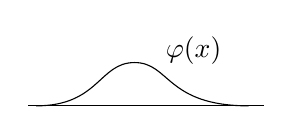
\begin{tikzpicture}[x=1cm,y=1cm]
\draw (0,0) -- (3,0);
\draw (0.1,0) .. controls (0.9,0) and (0.9,0.55) .. (1.35,0.55)
.. controls (1.8,0.55) and (1.75,0) .. (2.8,0);
\node at (2.1,0.7) {$\varphi(x)$};
\end{tikzpicture}
\end{adjustbox}
\end{center}
$S(x)$ может быть $S(x)=px$.
\SourceFigure{GELFAND-P000041}{wave-packet}{Осциллирующая кривая между двумя огибающими над и под горизонтальной линией; внутренние колебания и крайние штрихи требуют сверки с оригиналом.}
Колеб. (быстрые), \Unclear{GELFAND-P000041}{caption-contraction}{пропод. / пропорц.} $\varphi$.

\SourcePage{GELFAND-P000042}{unlabelled}
Асимпт. при $h\to0$ ищ. в виде
\begin{equation*}
\Psi=e^{\frac{i}{h}a(x,t)}.
\end{equation*}
$a$ — компл. ф-я.
Подставим и получ. послед. ас. ф-лы решения зад.
Первые 2 члена имеют вид
\begin{equation*}
\Psi(x,t)=
\frac{\varphi(X(x,t))}{\sqrt{\frac{\partial x(X,t)}{\partial X}}}
e^{\frac{i}{h}\left(S(X(x,t))+\int p\,dx\right)+O(h)}
\end{equation*}
\Unclear{GELFAND-P000042}{remainder}{Положение $+O(h)$ в верхней строке: записано на уровне показателя экспоненты.}
[От знаменателя: — из унит.; см. Титчмарш и Ландау.]
$\varphi$ — зад. нач. амплит.
$X$ при $t=0$ $=x$.
$X$ — [зачёркнуто: точка, из к-рой надо].
\Unclear{GELFAND-P000042}{cancelled-origin}{В зачёркнутой строке: «точка, из к-рой надо»; последнее слово читается неуверенно.}
[Слева ниже: $(x,t)$.]
Классич. нач. условие.
\begin{equation*}
p=\dot{x},\qquad \dot{x}=\frac{\partial S}{\partial x}
\end{equation*}
$S$ в нач. мом. задано.
$n$-мерн. пв.
\SourceFigure{GELFAND-P000042}{phase-figure}{Оси $p$ и горизонтальная ось; кривая с вертикальными отрезками к $X$ и $x$, внутри «вр. $t$». Небольшой наклонный штрих у кривой и точная направленность требуют проверки.}
Ф-ла квазиклассич., справедл., когда якоб. $\neq0$.
\underline{Квазикл.} — когда справ. эта ф-ла.
\begin{equation*}
\ddot{x}=-\frac{\partial U}{\partial x}
\end{equation*}
классич. механика ($x$ — вектор).
В квант. мех. $\forall t$ есть волн. ф-я $\Psi$.
$|\Psi|^2$ — вер.
Ур-е движ. — Шрёд.
\begin{equation*}
\frac{i}{h}\frac{\partial\Psi}{\partial t}
=\Delta\Psi-\frac{U(x)}{h^2}\Psi
\end{equation*}
(если нет $i$, то ур-е теплопp.;
если нач. в точке, то потом расплывается).
Связ. с асимпт. соб. знач.
$\left.\Psi\right|_{t=0}$ задаётся. $\Psi(x)$ —.

\SourcePage{GELFAND-P000043}{22}
$S(x)=px$ тогда ф-ла де Бройле.
\begin{equation*}
\frac{\partial S}{\partial x}=p
\end{equation*}
Обычн. приём нах. асимпт. — реш. ищ. в виде
\begin{equation*}
e^{\frac{i}{h}S_0(x^t)+S_1(x^t)+hS_2(x^t)+\cdots}
\end{equation*}
\Unclear{GELFAND-P000043}{exponent-variables}{Над $x$ во всех аргументах небольшой знак, похожий на $t$; возможно $x^t$ или $\dot{x}$.}
По времени [вписано сверху: дифф.] $\frac{1}{h^2}$ \ldots
Гл. член надо искать как $e^{\frac{i}{h}S_0(x)}$.
Если $S$ вещ., то осциллир., если компл., то есть уб.
Получ. ур-е 1-го пор. и 1-я ф-я вещ. и получ. осцилл.
Надо взять асимпт., поэтому 2 чл.
Теперь надо подбр. нач. данные к этой асимпт.
\Unclear{GELFAND-P000043}{localized-datum}{$\Omega$ или $\delta$}
нельзя, т.к. много постр. частот (сильно лок.).
\begin{equation*}
\varphi(x,t)e^{\frac{i}{h}S(x,t)}
\end{equation*}
если подст. туда, то для $S$ ур-е 1-го порядка
\begin{equation*}
\frac{\partial S}{\partial t}
=H\left(x,\frac{\partial S}{\partial x}\right),
\qquad H=U(x)+\frac{\dot{x}^2}{2}
\end{equation*}
к-рому соотв. обыкн. ур-е.
$\varphi$ — плотн. дин. сист. (как они движ. по кл. мех.).
Надо взять $x$ и для неё найти $X$, так что
наше ур-е через $t$ из $X$ придёт в $x$.
Точки несут с собой $\varphi$.
\SourceFigure{GELFAND-P000043}{trajectory}{Изгибающаяся кривая с отмеченными $X$ и $x$; около $X$ толстый ответвляющийся штрих. Его направленность не установлена.}
По $x$ дано $\dot{x}$ (дана дин. сист.).
При малых $t$ одн.
\begin{equation*}
\Psi=e^{iH}
\end{equation*}
унит.
$\mathcal{D}$ — якоб. доб. для унитарности.
$e$ — фаз. множ. с изм. амплит. крутится.
Раб. Маслова, когда $t$ произв., а не мало.
$t=0$ якоб. [зачёркнуто:
\Unclear{GELFAND-P000043}{cancelled-jacobian}{неразборчивое выражение}]
$=1$ (преобр. тожд.).
Волн. ф-я осциллятора. Маятник.
\SourceFigure{GELFAND-P000043}{oscillator}{На горизонтальной оси $x$ с $0$: параболическая дуга, колебания и огибающая; подписи «в кл. мех. волн. ф-я», «exp убыв.». Толстые пересечения и число колебаний неоднозначны.}

\SourcePage{GELFAND-P000044}{unlabelled}
Если $t$ велико, то может случиться, что
кривая нач. данных ($n$-мерн. пв.) переламывается.
\SourceFigure{GELFAND-P000044}{folded-data}{Верхний левый рисунок: несколько загибающихся кривых, пересекающие лучи, горизонтальная и почти вертикальная линии; отдельные стрелки и пересечения неуверенны.}
Если вертик. кас., то $\mathcal{D}=0$,
но потом 2 точки и ф-ла сохр. \Unclear{GELFAND-P000044}{preserved-punctuation}{(!) / (?)}, но
надо доб. слаг. по точкам
\Unclear{GELFAND-P000044}{phase-integer}{$\gamma_j$ или $n_j$}
— целое.
\begin{equation*}
\int p\,dx)+i\,\frac{\pi}{2}n_j
\end{equation*}
[Между $i$ и $\pi/2$ зачёркнут знак:
\Unclear{GELFAND-P000044}{cancelled-phase-sign}{неразборчиво}.]
\underline{Рез. Маслова} — найдены $\underline{n_j}$.
$n_j=\pm1$ из общих сообр.
Обойти около точки ветвл. в компл. плоскости,
этим можно сказ. $\oplus$ или $\ominus$.
Все рез. прим. и в \underline{оптике}.
\SourceFigure{GELFAND-P000044}{optical-rays}{Пересекающиеся лучи и кривая огибающая; толстая стрелка у касания. Точное соотношение пересекающихся штрихов не установлено.}
Лучи огиб. кривую.
Будем следить за фазой по лучу.
При малых $\lambda$ — будет скачок фазы $\pi/2$ в точке касания.
\underline{Ответ} $n_j$ — индекс Морса.
\SourceFigure{GELFAND-P000044}{trajectory-figure}{Оси $p$ и горизонтальная со стрелками; семейство кривых, точки $x_1$, $x_2$, $X$, подписи «через время $t$», «через $t$», «здесь вырожд.», «сопр. точки» и наклонная «нач. данных». Перекрытые штрихи, точная принадлежность подписи $x_2$ и верхний знак у вертикальной линии требуют оригинала.}
Траект. — есть реш. вар. задачи по
принц. наим. действия.
\begin{gather*}
\delta u=0\\
\delta^2u
\end{gather*}
квадр. форма. У неё есть индекс
[зачёркнуто:
\Unclear{GELFAND-P000044}{cancelled-index}{неразборчивое короткое слово}]
(число отр. квадр.).
Или [зачёркнуто:
\Unclear{GELFAND-P000044}{cancelled-conjugate}{неразборчивое слово}]
число сопряжённых точек.
1-я часть раб. \underline{Лере} посв. близким вопр.
След. раз Повзнер
\Unclear{GELFAND-P000044}{next-speakers}{Уанг; между именами зачёркнутое слово; и Брушлин. Над строкой: «группам».}

\SourcePage{GELFAND-P000045}{23}
\underline{Березин.}
\begin{equation*}
H=\frac{p^2}{2}+V(x)
\end{equation*}
(напр. $V$ — растёт).
Пусть пов. $p^2+V(x)=\mathrm{const}$ все ограничены.
Тогда асимпт. собств. [зачёркнуто:
\Unclear{GELFAND-P000045}{cancelled-eigenfunction}{ф-й}]
значений:
объём обл., где $H\leq n\pi h$ — асимптотика
[зачёркнуто:
\Unclear{GELFAND-P000045}{cancelled-asymptotic}{неразборчивое слово}]
соб. чисел.
\underline{Гельфанд И.}
\begin{equation*}
-y''+p(x)y=\lambda y
\end{equation*}
\begin{center}
\begin{adjustbox}{max width=\linewidth}
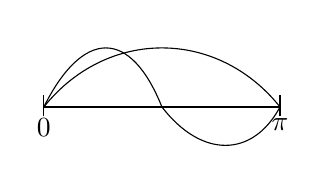
\begin{tikzpicture}[x=1cm,y=1cm]
\draw (0,0) -- (3,0);
\draw (0,-0.12) -- (0,0.15) node[below=5pt] {$0$};
\draw (3,-0.12) -- (3,0.15) node[below=5pt] {$\pi$};
\draw (0,0) .. controls (0.8,1) and (2.2,1) .. (3,0);
\draw (0,0) .. controls (0.5,1) and (1.1,1) .. (1.5,0)
.. controls (2,-0.65) and (2.65,-0.65) .. (3,0);
\end{tikzpicture}
\end{adjustbox}
\end{center}
\underline{На концах 0} [подчёркивание перечёркнуто].
$p=0$, собств. ф-и, $\lambda=-n^2$.
\Unclear{GELFAND-P000045}{lambda-sign}{Видимый знак $\lambda=-n^2$ сохранён.}
Утв. 1-я соб. ф-я не им. 0-й (инд. Морса 1).
2-я —//— им. один 0.
Это верно $\forall$ ур-ю.
Нули перемежаются.
Более точная теор. Если $y_0,\ldots,y_n$ соб. ф-я,
то
\begin{equation*}
\sum_{i=1}^{n}a_i y_i(x)
\end{equation*}
будет иметь $\leq n$ нулей!!
(похоже на многочлены).
[Зачёркнут определитель:]
\begin{equation*}
\det\begin{vmatrix}
y_0(x)&y_1&\cdots\\
y_0'(x)&y_1'&\\
\vdots&\vdots&\\
y_0^{(n)}(x)&y'(x)&
\end{vmatrix}
\end{equation*}
\Unclear{GELFAND-P000045}{cancelled-determinant}{В зачёркнутом определителе нижний второй элемент похож на $y'(x)$; индекс и порядок производной не установлены.}
Это экв. условию
\begin{equation*}
\begin{vmatrix}
y_0(x_0)&y_1(x_1)&\cdots\\
y_0'(x_0)&y_1'(x_1)&\cdots\\
\vdots&\vdots&\\
y_0^{(n)}(x_0)&y_1'(x_1)&
\end{vmatrix}\neq0
\end{equation*}
\Unclear{GELFAND-P000045}{mixed-determinant}{Второй элемент второй строки переписан; нижний второй элемент выглядит $y_1'(x_1)$, без видимого $(n)$.}
Или
\begin{equation*}
\begin{vmatrix}
y_0(x_0)&y_1(x_0)&\cdots\\
y_0(x_1)&y_1(x_1)&\cdots\\
\vdots&\vdots&\\
y_0(x_n)&y_0'(x_n)&
\end{vmatrix}\neq0
\end{equation*}
\Unclear{GELFAND-P000045}{value-determinant}{В нижнем втором элементе видны $y$, похожий на $0$ индекс и штрих: $y_0'(x_n)$; возможен иной индекс.}
[Над ним:] это 1-я соб. ф-я $\neq0$;
ур-я 2-го пор., \Unclear{GELFAND-P000045}{determinant-caption}{к-рая / к-рым}.
Отсюда лин. комб. $\leq n$ нулей, если $x_0<x_1<\cdots<x_n$.
Петров. чтобы
\begin{equation*}
\frac{\partial^2u}{\partial x_1^2}
-\frac{\partial^2u}{\partial x_2}-\cdots
+\left(p(x_1)+p(x_2)\ldots+p(x_n)\right)u=\lambda u
\end{equation*}
\Unclear{GELFAND-P000045}{petrov-equation}{У второго знаменателя виден $x_2$ без квадрата; справа $u=$ на краю, ниже $=\lambda u$.}
Соб. ф-и перем. разделяются.
Соб. ф-и $u_1(x_1)u_2(x_2)\ldots u_n(x_n)$.
1-я соб. ф-я $\neq0$.

\SourcePage{GELFAND-P000046}{unlabelled}
\underline{Намечено.}
\Unclear{GELFAND-P000046}{planned-speakers}{1° И. Бернштейн / Ф. Н. Бернштейн и С. Гильфанд}
[Справа отдельно:] \underline{Дайсон}.
$2^\circ$. Новиков, о раб. \underline{Адамса}.
$3^\circ$. Дынкин.
$4^\circ$. Винберг.
$5^\circ$. Пятецкий-Шапиро.
[Зачёркнуто:
\Unclear{GELFAND-P000046}{cancelled-heading}{неразборчивый заголовок}.]
\underline{Пят.-Шапиро}.
Зад. Клейна и Серра.
Рассм. гр. целочисл. матриц $n$-го пор. $\Gamma(n)$ с $\det=1$.
[Зачёркнуто: Как]
опис. все подгр. $\Gamma'$ конечного индекса?
\underline{Прим.}
\begin{equation*}
\Gamma(n,N),\qquad A\equiv E\pmod N
\end{equation*}
\Unclear{GELFAND-P000046}{congruence-index}{Под $\Gamma(n,N)$ небольшая подпись, похожая на $\lambda ij$ или $i,j$; под $A\equiv E$ — «не гр.» или «на гр.».}
(на диаг. сравн. с $1$, а вне диаг. делится на $N$).

\SourcePage{GELFAND-P000047}{35}
Все ли это подгруппы?
Всегда ли $\Gamma'$ содержит $\Gamma(n,N)$
(конгруенц.-подгруппу).
При $n=2$ это не так (Клейн).
$n\geq3$ это так (Серр).
\underline{Связь с группами Ли.}
Рассм. матрицы
\begin{equation*}
\begin{pmatrix}
1&0&&\\
&\ddots&1&0\\
0&&&1
\end{pmatrix}
\end{equation*}
[Зачёркнут символ:
\Unclear{GELFAND-P000047}{cancelled-elementary}{неразборчиво}.]
$E_{ke}=(\mathrm{ед.}+E_{ke})$.
\Unclear{GELFAND-P000047}{elementary-matrix}{Слева и справа один и тот же видимый $E_{ke}$; нижний второй индекс похож на $e$ или $\ell$.}
Гр. $\underline{\Gamma(n)\text{ ими порождается.}}$
Возьмём эти матр. и сопр. и возв. в степ. $N$:
$E_{ke}^{N}$, $\Gamma^{N}$.
При $n=2$ она беск. индекса;
$n\geq3$ кон. индекса.
$\Gamma/\Gamma^{N}$.
\fbox{$n=2$}
$N=2,3,4,5$ конечна, 6 1
\Unclear{GELFAND-P000047}{surface-abbreviation}{коммут. / коннут.}
$\Gamma/\Gamma^{N}=$ фунд. гр. поверхности,
$p=p(N)$, простая формула.
Серр, Лазар, Басс (1964).
Рассм. $a\equiv b\ (N)$, тогда при
\Unclear{GELFAND-P000047}{rank-overwrite}{$n\geq3$ / $N\geq3$}
в $\Gamma/\Gamma^{N}$ есть преобр. $a\to b$ (элем. преобраз.).
Потом когом. техника.

\underline{Гельфанд.}
Завтра на конф. по элем. частицам будет рассм.
[Зачёркнуто:
\Unclear{GELFAND-P000047}{cancelled-particles}{неразборчивое обозначение}.]
\fbox{$SU(3)$}.
Изв.-част. объед. в группы, преобр. друг в друга (мультиплеты).
Другая предст. $SU(3)$.
Идея $SU(2)\underset{\text{почти}}{\approx}SO(3)$.
[Над строкой: фн. лин. комб.]
Объед. с помощью \underline{$SU(2)\times SU(3)$}.
Гипотеза изв. и по $SU(6)$.
\underline{Замеч.} — в самом деле Лоренц. группа (с пар. перемещ.)
(группа Пуанкаре).
[Зачёркнуто:] $SU(2)\longrightarrow$ гр. Пуанкаре.
Раб. \underline{Тодорова}.
\underline{Кадышевский, Мурадян, Тавхелидзе.}
Вместо $SU(6)$ — 108 парам. группу.

\SourcePage{GELFAND-P000048}{unlabelled}
Salam предл. 144-пар. группу.
Fulton, Wess.
Гр. 2-х ступ. с комм. норм. делителем.
$SU(3)\otimes SU(2)$ в как. смысле.
Лор. преобр. — компл. матр.
\begin{equation*}
\begin{pmatrix}\alpha&\beta\\\gamma&\delta\end{pmatrix},
\qquad \det=1
\end{equation*}
(спинорное предст. гр. Лоренца).
\underline{Гр. Пуанкаре.}
\begin{equation*}
A=\begin{pmatrix}\alpha&\beta\\\gamma&\delta\end{pmatrix}
\end{equation*}
\underline{Вектор} — эрм. формы 2-го пор.
\begin{equation*}
H=\begin{pmatrix}a&b\\\bar b&c\end{pmatrix}
\end{equation*}
век. в 4-х мерн. пр-ве; $a,c$ — вещ., $b$ — компл.
\begin{equation*}
H\to AHA^*
\end{equation*}
Лор. $\det$ сохр.
Гр. Пуанкаре
\begin{equation*}
\begin{pmatrix}A&H\\0&A^{*-1}\end{pmatrix}
\end{equation*}
Это группа при
\Unclear{GELFAND-P000048}{h-zero}{$H=0$ или $H\geq0$}
вращ. ($H$ сдв.).
$H=1$ — пар. перем.
[Зачёркнуто:
\Unclear{GELFAND-P000048}{cancelled-group}{гр. Вращ. / гр. Лоренца}.]
Матр. 4-го порядка.
\begin{equation*}
\begin{pmatrix}A&H\\0&A^{*-1}\end{pmatrix}\otimes SU(3)
\end{equation*}
получ. полупрост. гр. с радик. (108-парам.).
Можно опис., что \underline{нужно}, \underline{чтобы реш. теор.} элем. частиц).

\underline{15/II. Каждан.}
Рез. Палам. в чисто алг. терминах.
Пусть $A$ — [зачёркнуто, сверху вписано: область]
целостности (кольцо без дел. нуля), $I$ — прим. идеал.
\Unclear{GELFAND-P000048}{domain-cancellation}{Под вписанным «область» зачёркнутое слово не установлено.}
\begin{equation*}
I\supset J
\end{equation*}
[Под $J$:] простой.
И пусть $J\supset I^2$ [зачёркнуто: $\neq$] $0$.
\Unclear{GELFAND-P000048}{ideal-powers}{Источник вводит $I$ как прим. идеал, но «простой» стоит под $J$; в $J\supset I^2$ зачёркнут знак перед $0$.}
Каждый такой идеал зад. дифф. опер. 1-го пор.

\SourcePage{GELFAND-P000049}{36}
Дифф. опер. — \Unclear{GELFAND-P000049}{linear-glyph}{$k$ / $A$ / $K$}-лин. опер.
\begin{equation*}
D(a\cdot b)=aD(b)+D(a)b
\end{equation*}
Идеал — 0 нек-рого наб. дифф. опер.
Пусть $A/J^2$ (1-го пор. из-за $J^2$).
Оператор не в кольцо, а в кольцо $A/J$.
Дифф. внизу, а отв. на подмн.
$aD(b)$ — умн. на $a$.
На $J$ опер. $A$-линейный [снизу: дифф.].
Наоборот, каждый $A$-лин. опер. на $J$
[зачёркнуты штрихи перед стрелкой:]
\begin{equation*}
J\overset{f}{\longrightarrow}A/J
\end{equation*}
Тогда его можно домн. на элем. $b$, снова лин.
[Сверху: $bf$.]
$\exists b$, что $bf$ продолжается до дифф. всего кольца.
Отсюда всё следует.
Будем рассм.
\Unclear{GELFAND-P000049}{field-notation}{$J(?)$ над полем частных}
Сущ. функционалы, вид. $J$ леж. в кольце частных.
Домн. на $b$ (т.к. нет дел. 0, то
[зачёркнут короткий знак:
\Unclear{GELFAND-P000049}{cancelled-field-symbol}{неразборчиво}]
кольцо ч.).
Если $A/J$ поле, тогда $\forall$ ф-л прод. до диффер.
(Надо взять локализацию $A/J$).
Сущ. отобр. поля
\begin{equation*}
A/J\longrightarrow A
\end{equation*}
[Под стрелкой: гом.]
чтобы обр. гом. был тождеств.
\begin{equation*}
A/J\longrightarrow A\longrightarrow A/J
\end{equation*}
[Зачёркнуто:
\Unclear{GELFAND-P000049}{cancelled-word}{Док-во.}.]
Пока произв.
$A/J\subset A$, $J\subset A$.
Любой эл. расклад. в $\Sigma$ ($\Sigma$ как лин. пр-во).

\SourcePage{GELFAND-P000050}{unlabelled}
На $J$ он уже задан.
Лин. отобр. $J\to A/J$ прод. на всём 0.
Трансценд. эл. куда угодно.
\begin{gather*}
y\to\hat y,\qquad x^2=y\\
\hat x'^{\,2}-\hat y=i_1;\qquad
\hat x=\hat x'+i_2;\\
\hat x^2=\hat x'^{\,2}+2\hat x'i_2
=\hat y+2\hat xi_2+i_1
\end{gather*}
\Unclear{GELFAND-P000050}{square-expansion}{В записи нет $i_2^2$; во втором равенстве $\hat x$ без штриха, в первом со штрихом.}
Отсюда $i_2$ находится (т.к. $A/J$ поле).
\underline{Вместо $I$ писалось $J$ и наоборот.}
Общ. вид дифф. опер. в кольце мног.
\begin{equation*}
\sum P_i(x_1,\ldots,x_n)\frac{\partial}{\partial x_i}
\end{equation*}
$P_i$ — многочлены.
\underline{Алгебр. теория дифф. ур-й над произв. полем.}
Дьёдонне, Гротендик: перешли в алг. зад. к произв. полю.
\underline{Обыкн. ур-е.}
\begin{gather*}
\frac{dx}{dt}=P(x,y)\\
\frac{dy}{dt}=Q(x,y)
\end{gather*}
[В числителе первого уравнения переписана буква.]
$t$ замен. лок. кольцом $\forall$ точке ($t$ лок. параметр).
\begin{gather*}
x=\sum a_k t^k\\
y=\sum b_k t^k
\end{gather*}
Дифф. ур-я над $\underline{P^2}$.
\Unclear{GELFAND-P000050}{differential-field}{Буква $P$ с показателем 2; возможно $P^2$ или $p^2$, без видимого двойного штриха.}
\begin{equation*}
D(x(t))=f(x(t))
\end{equation*}
$D$ — дифф. оператор в кольце элем. $x$.
Окольцованное пр-во. Точки $(x,y)$ и \underline{слои}.
$\forall$ точке кольцо.
Слой над каждой точкой — степ. ряд от $t$
($\forall$ точке степ. ряд от $t$).
\SourcePage{GELFAND-P000051}{37}
\begin{equation*}
Da=b.
\end{equation*}
\Unclear{GELFAND-P000051}{upper-equation-letter}{В левой записи $a$ / $\alpha$; отдельного определения на этом кадре нет.}
Нач. усл. --- знач. в макс. идеал.
Потом локализовать.
$D$ перен. на любую локализацию.
Реш. должно быть идеалом. (?)
Всё кольцо не надо зад. Оно изв. локально.
$x$ и $y$ не надо задавать.

\underline{Паламодов.}
\begin{equation*}
\mathcal P\quad\text{--- кольцо мн.}\qquad P(z_1,\ldots,z_n).
\end{equation*}
[Перед $P$: \Unclear{GELFAND-P000051}{polynomial-cancellation}{густо зачёркнут короткий символ}.]
$\mathcal H$ --- пр-во всех ф-й в обл. голом. (напр. шара).
\begin{equation*}
\mathcal J\subset\mathcal P.
\end{equation*}
Прим. идеал с базисом $P_1,\ldots,P_t$.
Рассм. $\mathcal J\mathcal H$.
Факторпространство $\mathcal H/\mathcal J\mathcal H$.
Строится $\mathcal H\{\mathcal J\}$, ему изоморфное,
с пом. оператора $d(z,D)$.
\begin{equation*}
\mathcal H\{\mathcal J\}=\bigl\{h(z)\big|_N\quad
\forall\zeta\in N\quad\exists F_\zeta(z)\quad
f(z)=d(z,D)F(z)\big|_N\bigr\}.
\end{equation*}
\Unclear{GELFAND-P000051}{local-function-letter}{Первый символ функции в фигурной скобке похож на $h$ / $f$; справа написано $f(z)$. Буквенное несогласование не исправлено.}
\Unclear{GELFAND-P000051}{local-condition-symbols}{Знак точки под $\forall$ и индекс $F$ похож на $\zeta$ / $\xi$; буква оператора в $d(z,D)$ похожа на $d$ / $\delta$. Правая формула тесно подходит к краю кадра; видимая нижняя $N$ сохранена.}
\Unclear{GELFAND-P000051}{vector-annotation}{Под первым $h(z)$: вектор. комп. / конх. / конк., см. / ан. / лин. опер. в наб. $d$ / $\lambda$ [сокращения неуверенны; «комп.» сильнее после повторного чтения].}
[Под $F_\zeta(z)$: аналит. в окр.]
Локальная теорема. Есть теор. с оц. роста.
\underline{Рез.}
\begin{equation*}
\mathcal H\{\mathcal J\}\cong\mathcal H/\mathcal J\mathcal H.
\end{equation*}
Изом. естественный.
[Под «изом.» стрелка вправо; под «естественный» отдельная толстая линия.]

\SourcePage{GELFAND-P000052}{unlabelled}
\underline{Дынин.} $X$ --- комп. многообр.
Над ним вект. рассл. $E_0$, $E_1$.
\begin{equation*}
\begin{adjustbox}{max width=\linewidth}
\begin{tikzcd}
E_0\arrow[dr]&&E_1\arrow[dl]\\
&X&
\end{tikzcd}
\end{adjustbox}
\end{equation*}
Пучок ростков $C^\infty$-ф-й 1-го и 2-го расслоения:
[Над ф-й вставлено: сечений.]
\begin{equation*}
\mathcal E(E_0),\qquad\mathcal E(E_1).
\end{equation*}
И морфизмы
\begin{equation*}
\mathcal E(E_0)\overset{A}{\longrightarrow}\mathcal E(E_1).
\end{equation*}
([Отмена: \Unclear{GELFAND-P000052}{morphism-cancellation}{короткая густо переписанная запись}; под ней «морф.»]
$\forall$ зад. дифф. операторами.)
Локально $\mathcal E(E_0)|_U$ --- гладкие вектор ф-и.
\begin{equation*}
\mathcal E(E_0)|_U\approx C^{n_0}(U),\qquad
\mathcal E(E_1)|_U\approx C^{n_1}(U).
\end{equation*}
[От первой строки стрелка вниз к $A(U)$ во второй.]
Дифф. опер. --- матрица. Символ --- главн. часть матрицы.
\underline{Локально} $\sigma(A)(x,\xi)$ --- гл. часть хар. матрицы.
\Unclear{GELFAND-P000052}{symbol-argument}{Второй аргумент $\sigma(A)$ густо переписан; видны формы $\xi$ / $\zeta$ / $D$.}
(Отбир. члены старшей степени.)
\underline{Формализовать.}
Кас. рассл. --- вект. $F$.
\begin{equation*}
\begin{adjustbox}{max width=\linewidth}
\begin{tikzcd}
&X&\\
&T(X)\arrow[u,"\pi"]&\\
\pi^*E_0\arrow[ur]\arrow[rr,"\sigma(A)"']&&\pi^*E_1\arrow[ul]
\end{tikzcd}
\end{adjustbox}
\end{equation*}
$A$ эллипт., если $\sigma(A)$ мономорфизм.
(См. Шварц.)
\underline{Пример.}
\begin{equation*}
E_0:\quad X\times\mathbf R^1\longrightarrow X.
\end{equation*}
[Под $E_0$: ф-и.]
\begin{equation*}
\mathcal E(E_0)=C(X)\qquad C^\infty\text{ --- ф-и от }X.
\end{equation*}

\SourcePage{GELFAND-P000053}{38}
\begin{equation*}
C(X)\overset d{\longrightarrow}C^1(X).
\end{equation*}
[Под $d$: внешн. дифф.]
Лок. $f(x)\longrightarrow\operatorname{grad}f(x)$.
\underline{Символ} --- умн. на вектор $\xi\in T(X)$.
Это пример переопр. эллиптич. системы.
\begin{equation*}
f(x)\overset d{\longrightarrow}\sum\frac{\partial f}{\partial x_i}\,dx_i.
\end{equation*}
\begin{equation*}
f(x)\longrightarrow
\begin{pmatrix}\dfrac\partial{\partial x_1}\\\vdots\\\dfrac\partial{\partial x_n}\end{pmatrix}f(x).
\end{equation*}
\begin{equation*}
E_0=X\times\mathbf R\longrightarrow X,\qquad
E_1:\ \Lambda T(X)\longrightarrow X.
\end{equation*}
\Unclear{GELFAND-P000053}{form-bundle}{После $E_1$ плотная отмена перед двоеточием; знак перед $T(X)$ похож на $\Lambda$ / $\wedge$. Ясная звезда при $T$ не видна.}
Дифф. формы --- сеч. такого рассл.
\underline{Результат.}
\begin{equation*}
\mathcal E(E_0)\overset A{\longrightarrow}\mathcal E(E_1).
\end{equation*}
Возьмём
\begin{equation*}
0\longrightarrow\ker A\longrightarrow\mathcal E(E_0)
\overset A{\longrightarrow}\mathcal E(E_1).
\end{equation*}
Если $A$ --- эллипт., то
\begin{equation*}
\dim H^i(X,\ker A)<\infty.
\end{equation*}
\underline{Частные случаи.}
1°. Пусть $A$ --- эллипт. по Петровскому.
\begin{equation*}
\mathcal E(\mathbf R^n)\overset A{\longrightarrow}\mathcal E(\mathbf R^n).
\end{equation*}
Тогда пр-во глоб. решений конечномерно.
\begin{equation*}
H^0\quad\text{--- конечно.}\qquad H^1\quad\text{--- дефект. (кон. дефект)}
\end{equation*}
\begin{equation*}
H^1(X,\ker A).
\end{equation*}
2°. Опер. внешн. дифф.
\begin{equation*}
\dim H^i(X,\ker d)\quad\text{--- числа Бетти.}
\end{equation*}
[Под $\ker d$: пучок const.]
3°. Компл. ан. Теор. Картана--Серра--Кодаира.

\SourcePage{GELFAND-P000054}{unlabelled}
\underline{Доказательство.}
[В заголовке несколько букв переписаны густо.]
(Читать Годеман, Картан и Ейленберг; Маклейн [вписано ниже внутри скобки].)
$\mathcal P$ --- пучок. Как счит. гомологии.
\begin{equation*}
0\longrightarrow\mathcal P\longrightarrow\mathcal P_0\longrightarrow\mathcal P_1\longrightarrow\cdots.
\end{equation*}
Тонкая резольвента.
\begin{equation*}
0\longrightarrow\mathcal P_0(X)\overset{d_0}{\longrightarrow}\mathcal P_1(X)\overset{d_1}{\longrightarrow}\cdots.
\end{equation*}
[Под $\mathcal P_0(X)$: \underline{сечения}.]
\begin{equation*}
H^1(X,\mathcal P)=\ker d_1/\operatorname{Im}d_0.
\end{equation*}
\begin{equation*}
0\longrightarrow\ker A\longrightarrow\mathcal E(\mathbf R^n)\overset A{\longrightarrow}\mathcal E(\mathbf R^n).
\end{equation*}
Это тонкая резольвента.
$H^1$ --- фактор.
Остальные для опер., элл. по Петр., 0.
[Слева зачёркнуто: «Идея»; рядом \underline{Док-ва}. От подписи стрелка вниз.]
[Длинная овальная/ступенчатая рамка:]
Главн. наша зад. об эйлеровой хар-ке (альтерн. суммы).
2 способа.
\underline{Кодаира:} пр-во реш. элл. ур-я.
Свед. к лемме Шварца,
[под строкой волнистая линия и стрелка вниз к:]
не перен. высс. гом. (нет теор. $A$ и $B$).
\Unclear{GELFAND-P000054}{second-method}{Друг. способ введ. / ввод. топ. / тон. и вп.-непр. тожд. опер. [Первые сокращения не раскрыты.]}
Резольв. из бан. пр-в.
\underline{Банаховский пучок.}
Пучок $\mathcal P$: $U\longrightarrow\mathcal P(U)$ (предпучки).
Типа Фреше. $\mathcal P(U)$ --- $F$-пр-ва, а огр. отобр. непр.
Серии новых пучков
\begin{equation*}
C^{p,r}(\mathcal P).
\end{equation*}
\begin{equation*}
U\longmapsto C_U^{p,r}(\mathcal P(U)).
\end{equation*}
Вект. значн. дифф. формы степ. $p$, гладкости $r$.
Пучок расщепляется,
\Unclear{GELFAND-P000054}{final-splitting}{но если нет фн. прдп. / прдл. [сокращения не установлены],}
то он не расщепляется.

\SourcePage{GELFAND-P000055}{39}
Для $\mathcal P=\mathcal E(E)$. Пучок --- пр-во Фреше.
Резольвента де Рама.
\begin{equation*}
0\longrightarrow\mathbf R\overset d{\longrightarrow}C^{0,r}
\overset d{\longrightarrow}C^{1,r}\overset d{\longrightarrow}\cdots.
\end{equation*}
[Под последовательностью длинная скобка; ниже \Unclear{GELFAND-P000055}{de-rham-cancellation}{короткий густо зачёркнутый знак}.]
Коэф. --- отобр. $U$ в дифф. формы.
Коэф. --- гл. отобр. $U\longrightarrow\mathcal P(U)$.
$r$ --- поряд. гладкости.
При перех. к пучку новых сеч. не добавим (но не в общ. случае, а при дан. предп.).
По типу резольв. де Рама
\begin{equation*}
0\longrightarrow\mathcal P\longrightarrow\widehat C^{p,r}(\mathcal P)
\overset d{\longrightarrow}\widehat C^{1,r}(\mathcal P)\longrightarrow\cdots.
\end{equation*}
\Unclear{GELFAND-P000055}{hat-resolution}{Первый верхний индекс у $\widehat C$ похож на $p$ / $0$; буква $p$ оставлена явно, без исправления по типу резольвенты.}
Подправл. из-за пор. гладкости.
Получ. банаховские пр-ва.
$H^i(X,\mathcal P)$ \Unclear{GELFAND-P000055}{cohomology-topology}{над. / нов. топ. [плотно переписанное сокращение].}
Оно не зав. от выб. резольвент.
\begin{equation*}
H^i(X,\mathcal P)^{(r)}\longrightarrow H^i(X,\mathcal P)^{(r-1)}.
\end{equation*}
Вз. одн. пр-ва Фреше (изоморфизм).
Он вп. непр. в силу теор. вложения.

\underline{Гельфанд.} Задача: $X$ --- комп., на нём пучок лин. топ. пр-в.
\underline{Прим.} $X$ --- точка. Просто пр-во.
Дифф. опер. --- \Unclear{GELFAND-P000055}{endomorphism}{эндом. в самёе / самёё себя [слово «эндом.» густо переписано; под ним вставлено и подчёркнуто «пучка»].}
(Смысл сохр.)
Когда оно конечн. индекса.
$X$ --- 1 точка. $E+$ вп. непр. Теор. Рисса.
Тогда можно рассм. операторы эллипт. $\infty$-порядка.
\underline{Дынин.}
Нужна гипоэллипт. оператора. В резольв. всё время один пучок $\ker A$.
Просто непр. коэфф., будет ли конечн. индекса?
\underline{След. раз.} Адамс (Новиков), Березин
\Unclear{GELFAND-P000055}{next-talk}{(РиО / РиЭ).}

\SourcePage{GELFAND-P000056}{unlabelled}
[В рамке: 22/II. Под датой \underline{Адамс.}]
\underline{Новиков С.П.} [Двойное подчёркивание.]
$S^n$: сколько лин. незав. вект. полей? (непр. п.)
[Под «сколько»: $\nu(n)$.]
\underline{Трив. факты.}
Есть на сф. неч. разм. ($\nu(n)\geq1$),
сф. чётных разм. нет ($\nu(n)=0$).
\begin{equation*}
\sum\text{инд. особ.}=\text{Эйлер. хар-ке.}
\end{equation*}
$M^n$ --- $n$-мерн. \Unclear{GELFAND-P000056}{vector-graph}{м-о. / м-ф. [последний знак сокращения густой].}
\begin{equation*}
(m,\varphi(m))\subset(M^n,\mathbf R^n),\qquad(m,T_m).
\end{equation*}
[Под первой записью: график. Под $(m,T_m)$: векторное поле.]
$(m,0)$ --- канонич.
Его индекс пересеч. --- есть инд. особенности.
[Под строкой волнистая скобка к \Unclear{GELFAND-P000056}{zero-section}{$c(m,0)$ / $\varepsilon(m,0)$}.]
(Здесь только 1 и $-1$, а степень $n$).
$E=2$ и потому полей нет.
2) $S^3$ и $S^7$ параллелиз.
\Unclear{GELFAND-P000056}{sphere-three-seven}{Перед следующими равенствами короткая зачёркнутая запись; верхний знак второй сферы похож на $7$ / звёздочку.}
$\nu(3)=3$, $\nu(7)=7$.
3) $\nu(2n-1)\geq1$ ($S^{2n-1}$).
4) Если на $S^{2m-1}$ есть $k$ нез. полей ($\nu(2m-1)\geq k$), то
на $S^{2pm-1}$ $\nu_{2pm-1}\geq k$.
Кратко:
\begin{equation*}
S^{m-1},\quad\nu_m\geq k\quad\Longrightarrow\quad S^{pm-1},\quad\nu_{pm-1}\geq k.
\end{equation*}
\begin{equation*}
\sum_{i=1}^m x_i^2=1.
\end{equation*}
[Под суммой: $\mathbf R^m$; справа $\mathbf R^{pm}$.]
Коорд. $p$ групп по $m$ штук.
\Unclear{GELFAND-P000056}{block-indices}{$x_i^{(j)}$ / $y_i^{(j)}$ [первый символ переписан], $i=1,\ldots,m$, $j=1,\ldots,p$.}
Пусть $p=2$.
\begin{equation*}
\sum y_i^2+\sum z_i^2=1^*.
\end{equation*}
[Под каждой суммой: $\mathbf R^m$. Звёздочка после 1 видима; сноски на кадре нет.]
\begin{equation*}
v(x)\text{ в }\mathbf R^m,\qquad v(x)\perp x\qquad(\text{поле на }S^{m-1}).
\end{equation*}
\Unclear{GELFAND-P000056}{bottom-vector-sign}{Начальная буква в $v(x)$ похожа на латинскую $v$ / $\nu$; отдельный знак квантора не установлен.}

\SourcePage{GELFAND-P000057}{40}
Положим
\begin{equation*}
\widetilde v(y,z)=\left(\|y\|v\left(\frac y{\|y\|}\right),\ \|z\|v\left(\frac z{\|z\|}\right)\right).
\end{equation*}
$\|y\|$ чтобы бороться с $y=0$, всё во 2-е комп.,
по $\operatorname{mod}=1$, и $\perp(y,z)$.
Получаются из незав. полей незав. поля.
Так получ. Хопфовские поля.
(Справа можно пис. другие поля.)
Можно стаб. задачу: увел. разм.
[Зачёркнуто «Было».] Изв. классифик. [сложно стр.]
[Слева в овале $S^{m-1}$, из овала длинная стрелка вниз.]
\begin{equation*}
m=2^b(2a+1),\qquad b=c+4d,\qquad0\leq e\leq3.
\end{equation*}
\Unclear{GELFAND-P000057}{range-letter}{В границах $0\leq e\leq3$ средняя буква похожа на $e$ / $c$; соседнее $b=c+4d$ и формулы используют $c$.}
То изв. число полей \fbox{$2^c+8d-1$}.
\begin{equation*}
\nu_{m-1}\geq2^c+8d-1.
\end{equation*}
В случ. 3, 7 даёт max.
$b=0$ \Unclear{GELFAND-P000057}{parity-word}{(чётное --- трв. / прв.).}
$b=1,2,3$, \Unclear{GELFAND-P000057}{low-exponent-sign}{густо переписанный знак/стрелка вниз}, просто, но треб. ср-ва алг. топ.
$b\leq12$ --- Toda, но $m$ пор. 3000.
\underline{Адамс} [два волнистых подчёркивания] док. это во всех размерностях.
[Слева звёздочка:] Редуц. часть прим. Атьи и Тода. Это прив. к зад. на гом. гр. сфер.
Оконч.
\begin{equation*}
\nu_{m-1}=2^c+8d-1.
\end{equation*}
Нечётн. множ. роли не играет.
Здесь одно утв.: $m\uparrow$ в 6 раз, то число полей ув. на 8.
\Unclear{GELFAND-P000057}{growth-factor}{В множителе один знак $6$ / $8$; чтение $6$ сильнее при увеличении.}
$(d+1)$ --- это видно из констр. в периодичн. Ботта.
\Unclear{GELFAND-P000057}{bott-comment}{Для $1*$ / $1\times$ всё изв.}
2 пар. сф., потом периодичн. Ботта.
\begin{equation*}
\pi_i(BO).\qquad
\begin{array}{c|cccccccc}
i&1&2&3&4&5&6&7&8\\
 &*&*& &*& & & &*
\end{array}
\end{equation*}
Где $\pi_i$ грассм. мн. нетрив.
[«Где» и $\pi_i$ подчёркнуты отдельно.]
$\mathbf RP^k$ --- проект. пр-во.
[Слева: Рассм.]
\begin{equation*}
K_{\mathbf R}(\mathbf RP^k)=\mathbf Z+\widetilde K_{\mathbf R}^{0}.
\end{equation*}
[От второго слагаемого длинная фигурная/волнистая скобка вниз к:]
\begin{equation*}
K_{\mathbf R}=\mathbf Z_{2^{f(k)}}.
\end{equation*}
\Unclear{GELFAND-P000057}{k-theory-bottom}{В нижнем индексе видны $2$ и $f(k)$; расположение допускает $2^{f(k)}$ / $2f(k)$. Верхний малый знак у $\widetilde K$ похож на $0$.}
$K$-функтор см. \Unclear{GELFAND-P000057}{reference-word}{«Матен.» / «Матем.»}. Атья и Хирцебрух.

\SourcePage{GELFAND-P000058}{unlabelled}
Элем. $K$ --- вещ. вект. расслоение, но с отнош. экв.
Слож. --- прям. $\Sigma$. Умн. --- тензорное пр. 2 вект. рассл.
1 элем. в $K$, если
\begin{equation*}
O_{N_1}\oplus\eta=O_{N_2}\oplus\zeta\quad\Longrightarrow\quad\eta\overset K\sim\xi.
\end{equation*}
\Unclear{GELFAND-P000058}{stable-equivalence}{После второй суммы знак похож на $\zeta$; после эквивалентности похож на $\xi$ / $\zeta$. Буквенное различие сохранено.}
\begin{equation*}
\underline{O_N=X\times\mathbf R^N.}
\end{equation*}
\Unclear{GELFAND-P000058}{induction-note}{(Можно подгруппы / индукция [слово переписано и не установлено]).}
Рассл. с точн. до экв. --- элемент $K$-функ.
\Unclear{GELFAND-P000058}{covariant-word}{Совок. / Сован.} --- $K$-функтор. Можно складывать, перемн.!
Трив. рассл. ($\Sigma$ кас. и норм. --- трив., есть обр. элем.)
Кажд. пр-ву став. в соотв. кольцо.
\underline{Над сферой} $K$-функтор
\begin{equation*}
K_{\mathbf R}(S^i)=\pi_i(BO).
\end{equation*}
(Сколько гом. отобр. в гр. мн.)
$K$-функт. сф. --- рассл. большой разм.
[Над «большой»: гр. мн.]
$BO$ --- грассм. мн. --- $n$-мерн. лин. в $N$-м. пр.
($n$ и $N$ велики). Всё стабилизируется [последние буквы перечёркнуты].
Вект. рассл. с зад. базой $\longleftarrow$ окрест. $\pi_i$.
Мн. соотв. клас. стягив. отобр.
Норм. пучку --- норм. сф. отобр. Далее искусств. приём.
$\mathbf RP^k$ разб. на клетки (по 1-й в каждой разм.).
Все вект. рассл. над $\mathbf RP^k$ стр. так.
\begin{equation*}
\sigma^i\quad\text{--- $i$-мерн. кл. }\mathbf RP^k.
\end{equation*}
\Unclear{GELFAND-P000058}{cell-bundle}{После $\sigma^i$ густо зачёркнута короткая запись; под ней $\mathbf RP^i\longrightarrow\mathbf RP^{i-1}$.}
Рассм.
\begin{equation*}
S^i=\mathbf RP^i/\mathbf RP^{i-1}.
\end{equation*}
[Ниже $\mathbf RP^k/\mathbf RP^{i-1}$; от него дугообразная стрелка вверх к предыдущему фактору.]
Все рассл. так получ.
Рассл. $S^i\longrightarrow$ рассл. над $\mathbf RP^i\longrightarrow$
[Стрелка в нижней строке доходит до правого края; следующий объект на этом кадре не виден.]

\SourcePage{GELFAND-P000059}{41}
$\longrightarrow$ рассл. на $\mathbf RP^k$.
$f(k)$ --- число звёздочек слева от $k$.
$\mathbf Z$ --- инвар. --- размерность.
Крит. точки появл. на циклах.
\begin{equation*}
\mathbf Z_{2^{f(k)}}\qquad\text{циклич. гр. пор. }f(k).
\end{equation*}
\Unclear{GELFAND-P000059}{cyclic-order}{Индекс у $\mathbf Z$ допускает $2^{f(k)}$ / $2f(k)$; в подписи порядка видимо $f(k)$, без отдельной $2$.}
[Слева \Unclear{GELFAND-P000059}{upper-cancellation}{короткая густая отмена}.]
\begin{equation*}
\mathbf RP^k\subset\mathbf RP^{k+1}.
\end{equation*}
Есть норм. пучок --- лист Мёбиуса.
(Это образующая) группы.
Его надо $2^{f(k)}$ раз склад. с собой.
\SourceFigure{GELFAND-P000059}{normal-bundle-diagram}{Слева почти горизонтальная линия; пять поперечных стрелок: две слева вниз, следующие три вверх. Над линией две стрелки вправо: короткая слева и длинная справа. Под ней незамкнутая овальная дуга с разрывом внизу справа; её левый конец идёт вверх к линии и имеет стрелку, справа конец слабый. Буквенных подписей нет.}
\begin{align*}
\underline{\nu^2=1},\qquad&\lambda=\nu-1,\\
\lambda^2&=1+1-2\nu,\\
\lambda^2&=2(1-\nu),\\
\lambda^2=-2\lambda.&
\end{align*}
Мульт. структура.
\Unclear{GELFAND-P000059}{lambda-symbols}{Узкий знак в $\nu$ похож на $\nu$ / $v$ / $V$; некоторые знаки равенства переписаны. Последняя строка в округлой рамке.}
[\Unclear{GELFAND-P000059}{lower-cancellation}{Длинная густо зачёркнутая строка слева под формулами}.]
Есть $\mathbf RP^{n-1}\subset O_n$.
[Над правой частью две короткие горизонтальные черты.]
$S^n$ ставится на гиперпл. экваторы --- в ортог. группу.
Кас. пучок --- отобр.
\begin{equation*}
S^{n-1}\longrightarrow O_n.
\end{equation*}
\Unclear{GELFAND-P000059}{sphere-map-insertion}{Над стрелкой тесно вставлено $\mathbf RP^{n-1}$ / $\mathbf RP^n$ с дополнительным наклонным соединительным штрихом; часть знаков густая.}
В симм. точках одинаков.
Оно \underline{\underline{2-листно}}.
(Склейка на экваторе);
вращение вокруг неё (отражение вокр. него);
оси пр. пр-во.
[От скобки об отражении стрелка вниз к $O(n)$; перед $O(n)$ чёрный переписанный штрих.]
[Слева имя:]
\Unclear{GELFAND-P000059}{axis-name}{Альберт Солом. / Солн.}
Шварц.
[Рядом наклонная прямая снизу слева вверх вправо, утолщённая точка на середине; подпись «ось в $\mathbf R^n$».]
\begin{equation*}
\mathbf RP^{n-1}/\mathbf RP^{n-k-2}\longrightarrow O_n/O_{n-k-1}.
\end{equation*}
\Unclear{GELFAND-P000059}{quotient-map}{В левом нижнем показателе $n-k-2$ / $n-n-2$; стрелка между факторами густо переписана.}
В действ. влож.

\SourcePage{GELFAND-P000060}{unlabelled}
[1/III; под III короткая линия.]
\underline{В.П. Паламодов.} [Волнистое подчёркивание.]
$\mathcal P$ --- кольцо мн. в $\mathbf C^n$,
$\mathcal J\subset\mathcal P$ --- идеал, примарный,
$P_1,\ldots,P_s$ --- образ.
$\mathcal H$ --- кольцо целых ф-й
[\Unclear{GELFAND-P000060}{whole-functions-cancellation}{после «ф-й» густо зачёркнут короткий знак}]
вып. области.
$\mathcal H/\mathcal J\mathcal H$ описывается так
\begin{equation*}
\mathcal H\{\mathcal J\}=\{f|_N\quad f(z)=d(z,D)F_\zeta(z)\}.
\end{equation*}
\Unclear{GELFAND-P000060}{local-f-index}{Нижний индекс $F$ похож на $\zeta$ / $s$; лишний квантор в этом кадре не добавлен.}
[Под формулой: лок. часть.]
\begin{equation*}
\mathcal H/\mathcal J\mathcal H\cong\mathcal H\{\mathcal J\}.
\end{equation*}
Каждан гов., что это получ. алгебраически.
[Под «получ.» стрелка вправо и отдельное подчёркивание.]

[Слева большой чёрный кружок.]
\underline{Гельфанд.}
\underline{Пример Нельсона.} [Волнистое подчёркивание.]
2 самосопр. оператора $A$ и $B$.
Что \Unclear{GELFAND-P000060}{selfadjoint-question}{меряет / меняет} самосопр. опер.? (не симм. заданн.)
[На правом поле:]
\begin{equation*}
i\frac d{dx},\qquad y(a)=y(b).
\end{equation*}
\Unclear{GELFAND-P000060}{boundary-margin}{Ниже: «или ещё / везд. $=0$»; краткое слово и обозначение не установлены.}
По существу самосопр. $A$ (симм.), если
нет вект., ортог. ко всем вект. вида
\begin{equation*}
\overline z=Ax-ix,\qquad \widetilde z=Ax+ix.
\end{equation*}
\Unclear{GELFAND-P000060}{range-z-marks}{Над первым $z$ два горизонтальных штриха, над вторым короткий неровный штрих: $\overline z$ / $\widetilde z$.}
(Тогда [\Unclear{GELFAND-P000060}{criterion-cancellation}{короткая густая отмена}] то же $\forall$ компл. $\lambda$.)
Иначе $Ax-ix$ всюду плотны.
$A-iE$ им. обр. (в общем?: если замкнуты)
\begin{equation*}
\left(i\frac d{dx}\quad\text{не даже симмет.}\quad
\begin{array}{ll}
f(a)=f(b)&\text{по сущ. самосопр.}\\
f(a)=f(b)=0&\text{только симм.}
\end{array}\right)
\end{equation*}
[Под «по сущ. самосопр.» волнистая линия.]
$A$ и $B$ по существу самосопр.,
$\alpha A+\beta B$ по сущ. самосопр.,
$\alpha,\beta$ --- вещ.
\begin{equation*}
\forall f\in\text{обл. опред.}\qquad ABf=BAf.
\end{equation*}
\Unclear{GELFAND-P000060}{domain-cancellation}{Над областью определения густо переписана короткая запись; под ней изогнутая черта.}
Тем не менее $A$ и $B$ не перестановочны.
[Слева зачёркнуто и дважды подчёркнуто «Пример.»; справа от него двойная вертикальная черта.]
$A$ и $B$ перест., если \Unclear{GELFAND-P000060}{functional-calculus-word}{различн. / резольв.} ф-и от них перестан.
\begin{equation*}
(A-\lambda E)^{-1}.
\end{equation*}
[Под формулой: опер. ограничен.]
Перест. [\Unclear{GELFAND-P000060}{resolvent-cancellation}{густо зачёркнуто короткое слово}] и с $B$ означает,
что и эти опер.
\Unclear{GELFAND-P000060}{resolvent-final-word}{переменн. / перестан. [конечное сокращение не установлено].}
\begin{equation*}
e^{iA}\quad\text{--- унит.}\qquad e^{iB}\quad\text{не перестановочны}.
\end{equation*}
[\Unclear{GELFAND-P000060}{final-cancellation}{Короткая густо зачёркнутая запись}; рядом $(\forall\text{ огр. опер.})$.]

\SourcePage{GELFAND-P000061}{42}
\underline{Пример Нелсона.}
\SourceFigure{GELFAND-P000061}{nelson-grid}{Квадратная сетка с тёмной центральной областью и жирными точками; подписи 0, 1, 2, 3 вдоль нижней стороны, 1, 2, 3 слева и 2 справа. Наложенные штрихи у центра и точная склейка требуют оригинала.}
Из обл. между квадр. выбр. жирные точки.
Отрезки склеиваются.
Кажд. точка склеив. с точкой гран. ближ. по гориз. или верт.
Углы склеив. между собой. Получ. поверхн. рода
\Unclear{GELFAND-P000061}{genus}{4 / 1}
с одной выбр. точкой.
\begin{equation*}
X=\frac{d}{dx},\qquad Y=\frac{d}{dy}
\end{equation*}
$iX$, $iY$ — формально самосопр.
Они коммутируют.
Но соотв. опер. не коммут.
Выбр. меры 0
\Unclear{GELFAND-P000061}{selected-path}{значен. / значит.}
траект. попад. в вершины.
$e^X$ и $e^Y$ — унит. опер., к-рые не перестановочны.
\begin{equation*}
e^{\frac{d}{dx}}f(x)=f(x+1)
\end{equation*}
(ф-ла Тейлора).
Док. сначала для аналит. ф-й, потом для всего гильб.
пр-ва пред. перех. (опер. унитарный).
И надо её двигать.
\SourceFigure{GELFAND-P000061}{shift-square}{Квадрат с отверстием, заштрихованными нижними левыми участками и стрелкой к подписи «ф-я с … здесь». Точная граница поддержки и перекрытые линии не установлены.}
$e^Y$ — обл. на 1 вверх, $e^X$ прокрутится.
[Ниже отдельно:] $e^X$.
Ф-я с
\Unclear{GELFAND-P000061}{support-word}{компт. / комп.}
здесь.
Исключ. конечн. число траект.
$e^{tX}$ — сдвиг по траект. опер. $X$.
Локально всюду перестановочны.
Что будет с опер. Лапласа?
[Переписан штрих перед «опер.»:
\Unclear{GELFAND-P000061}{laplace-overwrite}{неразборчиво}.]
Индекс дефекта.
\begin{gather*}
\Delta f=if\\
\underline{\Delta=X^2+Y^2}
\end{gather*}
(это след. из теор. Нелсона).
Он не явл. самосопр. (имеет
решение $C^\infty$, гр. усл., а в точке только $\int$ квадрат).
Сами опер. сдвига опр. на $L^2$, а не на периодич. ф-ях.
\underline{3 оп.}
$e^{itA}$:
\begin{align*}
1^\circ&=\int_{-\infty}^{+\infty}\frac{e^{it\lambda}}{iA-\lambda}\,d\lambda\\
2^\circ&=\int_{-\infty}^{+\infty}e^{it\lambda}\,dE_\lambda\\
3^\circ&:\quad \frac{df}{dt}=iAf
\end{align*}
\Unclear{GELFAND-P000061}{resolvent}{В первой записи знаменатель $iA-\lambda$, без видимого нормирующего множителя перед интегралом.}
$U_{t,0}f_0=f$ — унит. опер.
[Под $U$: реш.]

\SourcePage{GELFAND-P000062}{unlabelled}
\underline{Синай. \Unclear{GELFAND-P000062}{heading}{Гомол. / Полож.} в дин. системах.}
У эргод. дин. сист.
[Зачёркнуто:
\Unclear{GELFAND-P000062}{cancelled-spectrum}{неразборчиво};
сверху: с дискр. сп.]
спектр всегда простой.
$M$, $\mu$, $\{S_t\}$ — однопар. гр. в $M$.
В \Unclear{GELFAND-P000062}{hilbert-notation}{$L^2_M$ / $L^2_H$}
однопар. гр. унит. опер.
\begin{equation*}
U_t f(x)=f(S_t x)
\end{equation*}
[Под $U_t$: простой.]
В эргод. случае каждое соб. знач. простое.
\underline{Лебеговский спектр:}
$\forall f$
\begin{equation*}
(U_t f,f)=\int e^{it\lambda}p(\lambda)\,d\lambda
\end{equation*}
($p(\lambda)$ — суммир.).
(Вообще всегда $\int e^{it\lambda}\,d\mu$, здесь $\mu$ абс. непр.).
\underline{Счётнокр. леб. сп.}:
$\exists$ ортог. $f_1,f_2,\ldots$
\begin{equation*}
(U_t f_i,f_j)=0\qquad(i\neq j)
\end{equation*}
и всё порожд.
Во всех изв. прим. спектр счётно-кр.
\underline{Прим. Пр. тора.}
\begin{equation*}
\begin{pmatrix}a&b\\c&d\end{pmatrix},
\qquad \det=1,\quad\text{целочисл.}
\end{equation*}
\begin{gather*}
x\longrightarrow ax+by\\
y\longrightarrow cx+dy
\end{gather*}
Надо найти автог. Разлож. в ряд Фурье и действ.
\begin{gather*}
f(x,y)\longrightarrow f(ax+by,cx+dy)\\
e^{2\pi i(mx+ny)}
\longrightarrow e^{2\pi i((am+cn)x+(bm+dn)y)}
\end{gather*}
На целочисл. реш. действует матрица.
Надо взять траектории
\begin{equation*}
(m,n)\longrightarrow S(m,n)=(m',n')
\end{equation*}
Траект. — гипербола.
\SourceFigure{GELFAND-P000062}{hyperbola}{Сверху две пересекающиеся оси; ниже две почти вертикальные кривые ветви, наклонная линия и толстое пересечение. Точные стрелки и принадлежность штрихов к ветвям неуверенны.}
Вещ. соб. знач. — сж. по одной оси
и растяж. по др. ($\det=1$).
\begin{equation*}
S^k\begin{pmatrix}m\\n\end{pmatrix}\longrightarrow\lambda
\end{equation*}
($\lambda$ — соб. знач.).
\Unclear{GELFAND-P000062}{frequency-limit}{Векторная запись $S^k(m/n)\to\lambda$ сохранена без добавленного нормирования.}
Волны стан. всё более густыми и напр.
Волны $\longrightarrow$ к соб. напр.
Пр-во разлож. на пр-ва ф-й с частотами на
гиперболах. На 1-й гиперболе.
Послед. ортог. вект., кажд. перех. в следующий.

\SourcePage{GELFAND-P000063}{43}
[Сверху: ряд отдельных точек.]
(Сдвиг на 1 в целочисл. т.)
Непр. лебеговский спектр. Со сх. Бернулли — характ. группы.
\underline{Теорема.} Мера $d\sigma(\lambda)$.
\begin{center}
\begin{adjustbox}{max width=\linewidth}
\begin{tikzpicture}[x=1cm,y=1cm]
\draw[->] (-1,0) -- (1,0);
\draw[->] (0,-0.65) -- (0,0.65);
\end{tikzpicture}
\end{adjustbox}
\end{center}
$\sigma\times\sigma$.
\begin{gather*}
\alpha=\lambda_1+\lambda_2\\
\beta=\lambda_1-\lambda_2\\
d\sigma(\lambda_1)\times d\sigma(\lambda_2)=d\sigma^2(\alpha)
\end{gather*}
[Под $d\sigma^2(\alpha)$: свёртка.]
\Unclear{GELFAND-P000063}{spectral-product}{Продукт мер при замене $(\lambda_1,\lambda_2)$ записан как $d\sigma^2(\alpha)$, без явного множителя по $\beta$.}
\Unclear{GELFAND-P000063}{date-sinai}{Переписанная дата: 8/III / 4/III / 1/III; ниже Я. Синай / 2. Синай.}
$M,\mu,\{S_t\}$.
Соб. ф-я
\begin{equation*}
U_t f_\lambda=e^{i\lambda t}f_\lambda
\end{equation*}
пост. по \underline{mod} (у эргод. системы).
\underline{15/III. Тодоров.} $SU$.
\underline{22/III-65. Через год в Москве будет матем. конгресс.}
(Март — апрель.)
[Что такое «простой корень»? Связь с матрицами.]
\underline{\Unclear{GELFAND-P000063}{surname-contraction}{Гелф. / Гельф.} Зад.}
1. Делать алг. геом. на некомм. кольцах!!
2. Алг. теор. дифф. ур-й.
\underline{Повзнер.} Малый параметр.
\underline{Березин.} О ф-ях многих переменных.
Надо изуч. не все ф-и, а специф. — встр. в теор. предст. и
в стат. физике.
\underline{Повзнер} «пожелание» к Березину.
\underline{Кириллов.}
Обычн. дин. сист. — время $R$ или $Z$. Можно
произв. группа сохр. меру. Классифик., инвар.?
[Перед «Спектр» зачёркнуто:
\Unclear{GELFAND-P000063}{cancelled-spectrum}{неразборчиво}.]
Спектр — мн-во неприв. предст., на к-рые
разлож. пр-во ф-й на $M$.
[Справа:]
$M$; $H$ — ф-и; $G$;
$U_g:f(x)\longrightarrow f(g^{-1}x)$ — унит. опер.
$H$ разлож. на неприв. компон., к-рые наз. спектром.
$G$ комм. — \Unclear{GELFAND-P000063}{representations-contraction}{прдпр. / прдпрд.} одномерны.
$G$ действ. эргодич. (нет инв. ф-й, кроме const).
Для комп. гр. все транзит. и св. к описанию
подгрупп.
\underline{Прим.} 1) Гордин и Уайтхед.
\begin{equation*}
G=\prod Z_2
\end{equation*}
\Unclear{GELFAND-P000063}{group-caption}{Некомм. группа / Некомп. группа.}
Послед. 0 и 1, конечн. число не 0.
$\sum$ обычн.
У неё реш. зад. опис. предст. вирт. подгруппы.

\SourcePage{GELFAND-P000064}{unlabelled}
2) Двоично-рац. числа на окр.
\begin{equation*}
e^{i\frac{2\pi k}{2^n}}
\end{equation*}
\Unclear{GELFAND-P000064}{dyadic-exponent}{В числителе переписанные штрихи: $2\pi k$ / $\pi k$.}
Счётная.
Двойств. гр. — 2-адич. числа.
На ней уже неком. факты.
Точ. спектр и непр. сп.
Возм., что [зачёркнуто:
\Unclear{GELFAND-P000064}{cancelled-function}{ф / неразборчиво}]
произв. ф-й, разлож. по участкам.
\SourceFigure{GELFAND-P000064}{sawtooth}{Два коротких пилообразных участка над горизонтальными подчёркиваниями; вертикальные крайние штрихи и точное число изломов неуверенны.}
Непр. сп. даёт ф-ю разлож.
по дискр. мн-ву.
\underline{Оследец}: было и для обычн. системы.
\underline{2-мерн. время.}
\begin{equation*}
\begin{pmatrix}a&b\\0&1\end{pmatrix}
\end{equation*}
Потоки Синая (оснащённые).
Непр. предст. мало:
одном. $|a|^{i\lambda}(\operatorname{sign}a)^\varepsilon$!
И одно беск.-мерное.
\underline{Связь с группой Лоренца.}
\begin{equation*}
\begin{pmatrix}a&b\\c&d\end{pmatrix}
\end{equation*}
Действ. на пр-ве Лобач. (верхн. полуплоскость).
Про факт. по [зачёркнуто:
\Unclear{GELFAND-P000064}{cancelled-discrete}{неразборчиво}]
дискр. подгр. Будет комп. отриц. крив.
Кос. пучок — 3-х мерн. комп. мн., на к-ром действует
эргодич. гр. Лоренца. Дискр. спектр из-за компактности.
\underline{Гомологии дин. систем.}
Оператор
\begin{equation*}
U_g=\alpha(x,g)f(xg).
\end{equation*}
Гомоморфизм тогда.
$\alpha(x,g)$ — коцикл. $|\alpha|=1$.
\begin{equation*}
\alpha\in Z^1(G,F).
\end{equation*}
[Под $F$: гр. функций.]
$\alpha$ эквив., если сущ. непрерыв. преобр.
Это быв., если
\begin{equation*}
\frac{\alpha}{\alpha_1}\in B^1(G,F)
\end{equation*}
Общ. вид границы
\begin{equation*}
\alpha_0(x,g)=\frac{\beta(xg)}{\beta(x)}
\end{equation*}
— гомолог. нулю.
$Z^1/B^1$ — гомологии.
Выч. лишь если гр. транзитивна (тогда
это мн-во предст. стаб. подгруппы).
Гом. 0 не все const, а $e^{2\pi it\lambda}$.
[Справа:] $\lambda$ из спектра.
Если подгр., то
гр. гом. опред. дин. систему.

\SourcePage{GELFAND-P000065}{44}
Совок. гом. наз. предст. вирт. подгруппы (хотя подгр. нет).
\underline{2-мерн. гом. спектра дин. системы.}
$f_\lambda$ — соб. ф-и.
Выб. 1 фикс. соб. ф-ю.
\begin{equation*}
f_\lambda f_\mu=C_{\lambda,\mu}f_{\lambda\mu}
\end{equation*}
$C_{\lambda,\mu}$ — 2-мерн. коциклы на спектре дин. системы.
\begin{equation*}
C_{\lambda,\mu}C_{\lambda\mu,\nu}
=C_{\lambda,\mu\nu}C_{\mu,\nu}
\end{equation*}
Эквивал. 1
\begin{equation*}
C_{\lambda,\mu}=\frac{a_\lambda a_\mu}{a_{\lambda\mu}}
\end{equation*}
В классич. случае эти гом. тривиальны («сист. опред. спектром»).
Неизв. даже опред. ли дин. сист. своим спектром для
кон. групп (Гельфанд счит., что нет).
\underline{Группа вращ. икосаэдра.}
\begin{equation*}
\begin{pmatrix}\alpha&\beta\\\gamma&\delta\end{pmatrix},
\qquad \alpha\delta-\beta\gamma'=1
\end{equation*}
\Unclear{GELFAND-P000065}{icosahedron-prime}{У $\gamma$ в условии определителя виден верхний штрих; $\gamma'$ / $\gamma$.}
$\alpha,\beta,\gamma,\delta$ по mod 5.
(В вершине 5 тр-ков.)
\underline{Клейн. Лекции об икосаэдре.}
\begin{equation*}
T_g f(x)=f(xg)
\end{equation*}
Надо восстановить $X$. Есть опер. сдвига, группа.
Но есть ещё опер. умн. на ф-ю (но если есть
кольцо, то предст. в кольце опред. дин. систему).
\underline{29/III. Виктор Николаевич.}
Связь между алгебрами Ли и ассоц. алгебрами.
\begin{equation*}
L\longrightarrow U
\end{equation*}
[Под $L$: алг. Ли; под $U$: универ. обёрт. алг.]
\underline{Хариш-Чандра} — если $L$ простая, то что можно сказать об $U$?
Проблема Джекобсона: что надо, чтобы $U$ была примитивной
(сущ. над ней точный неприв. модуль).
\underline{Пример.}
$e_1,e_2$, $[e_1,e_2]=e_1$ — $U$ примит.
$[e_1,e_2]=0$ — $U$ не-примит.
(Это кольцо мног., а коммут. примит. алг. — поле.)
$A^{(-)}$ — алг. Ли получ. из ассоц. алг. $A$ (ab-ba).
Какие св-ва $A$ перен. на $A^{(-)}$?
В $A$ — Ли-идеалы. \underline{Baxter.} Если $A$ — полупр. по Джекобсону.
Если $A$ — простая, то Ли-ид. тоже нет.
(Если нет об. идеалов, то нет и Ли-идеалов.)
\Unclear{GELFAND-P000065}{lie-ideal-claim}{Источник утверждает отсутствие Ли-идеалов у простой $A$; оговорки не дописаны.}

\SourcePage{GELFAND-P000066}{unlabelled}
\Unclear{GELFAND-P000066}{burnside-heading}{II / III}.
Проб. Бёрнсайда. Рез. Кострикина.
($A$ — алг.
[Зачёркнуто:
\Unclear{GELFAND-P000066}{algebra-overwrite}{неразборчиво};
под ним: ассоц.?]
$X$ — кон. мн-во,
[зачёркнуто:
\Unclear{GELFAND-P000066}{generating-overwrite}{неразборчиво}]
порожд. $A$, $[X]\supset X$.
[Под $[X]$: порожд. алг. Ли.])
\begin{equation*}
\exists\ [\text{зачёркнуто: }\forall]\ n,\qquad
e\subset[X],\qquad e^n=0.
\end{equation*}
\Unclear{GELFAND-P000066}{burnside-quantifiers}{$\exists\,n$, переписанный знак перед $n$; отношение $e\subset[X]$ / $e\in[X]$.}
Тогда $A$ нильпот. (т.е. $\forall$ элем. нильпотентен).
\underline{Гельфанд. Диксмье} — нереш. задача:
2 кольца $P(x,\frac{d}{dx})$ и
$P(x,\frac{d}{dx},y,\frac{d}{dy})$ (полиномы).
Изоморфны ли эти кольца?
\underline{С. Гельфанд. Дайсон.}
1. Ортог. ансамбль.
\begin{gather*}
U^T=U\\
UU^*=1
\end{gather*}
[Справа: симм. и унит.]
Инв. для унит. гр.
\begin{equation*}
U\longrightarrow VUV^T
\end{equation*}
(однор. пр-во унит. группы).
Плотн. распр. соб. знач.
$P(\theta_1,\ldots,\theta_N)d\theta_1\ldots d\theta_N$ —
мера матриц, соб. знач. (их арг.) в
$(\theta_1,\theta_1+d\theta_1);\ldots$.
Стаб. подгруппа:
$E\longrightarrow VV^T=E$ (вещ. ортог. матрицы).
Ввод. инв. мера.
Оказ.
\begin{equation*}
p_1(\theta_1,\ldots,\theta_N)
=C_1\prod_{i<j}|e^{i\theta_i}-e^{i\theta_j}|
\end{equation*}
2. Все унит. матрицы. (Вероятн. соб. значений!)
Группа — унит. [Внутр. автом.]
$U\longrightarrow VU$
[далее зачёркнут знак:
\Unclear{GELFAND-P000066}{unitary-action}{неразборчиво, похож на $V^*$}.]
\begin{equation*}
p_2(\theta_1,\ldots,\theta_N)
=C_2\prod_{i<j}|e^{i\theta_i}-e^{i\theta_j}|^2
\end{equation*}
(Инв. мера унит. гр. $\int$ по кл. сопр. элем.)
Более вероятны различные соб. знач.
[Над $\theta$: обведена буква:
\Unclear{GELFAND-P000066}{circled-symbol}{$\Delta$ / неразборчиво}.]
Рассм. все матр., $-\alpha<\theta<\alpha$ нет соб. значений.
\underline{Вероятность этого вычисляется.}
\begin{equation*}
R_\alpha(\alpha)=
\int_\alpha^{2\pi-\alpha}\int\ldots\int_\alpha^{2\pi-\alpha}
|e^{i\theta_i}-e^{i\theta_j}|^\beta
\,d\theta_1\ldots d\theta_N
\end{equation*}
\Unclear{GELFAND-P000066}{gap-integral}{В этой строке перед модулем нет уверенно видимого $\prod$; индекс $R$ похож на $\alpha$, аргумент $\alpha$ / $d$.}
$\beta=1,2$. У Дайсона $\forall\beta$.
Делаются физические предположения.
\underline{Физ. аналог.}
\begin{center}
\begin{adjustbox}{max width=\linewidth}
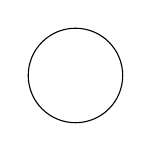
\begin{tikzpicture}[x=1cm,y=1cm]
\draw (0,0) circle[radius=0.6];
\end{tikzpicture}
\end{adjustbox}
\end{center}
Провод. нить в виде окр., на ней $N$ зарядов,
отталк. по 2-мерн. эл-стат.
Тогда энергия (потенц.) = $W$.
[Зачёркнуто перед суммой:
\Unclear{GELFAND-P000066}{energy-cancellation}{$\prod_{i<j}$ / неразборчиво}.]
\begin{equation*}
W=\sum_{i<j}\ln|e^{i\theta_i}-e^{i\theta_j}|
\end{equation*}
(Своб. заряды.)
С этим гр. кан. стат. функции.
\begin{equation*}
\int_0^{2\pi}\int_0^{2\pi}\ldots\int_0^{2\pi}
e^{[-\beta W]}\,d\theta_1\ldots d\theta_N
\end{equation*}

\SourcePage{GELFAND-P000067}{45}
$\beta=\frac1T$.
$T=1$ и $1/2$ соотв. ортог. и унит. ансамблю.
Кусок $(-\alpha,\alpha)$ запрещён.
\SourceFigure{GELFAND-P000067}{forbidden-arc}{Окружность с тёмным правым коротким участком между подписями $\alpha$ и $-\alpha$. Толстые конечные штрихи не позволяют установить стрелки.}
Своб. энергия.
\begin{equation*}
R_\beta(\alpha)=e^{\beta[F(\alpha)-F(0)]}
\end{equation*}
$F$ — своб. энергия.
(Это рав-во можно счит. её опр.)
Рассм. матрицы, не им. соб. знач. в инт.
$-\alpha<\theta<\alpha$.
Их вероятность
\begin{equation*}
\Psi_\beta(\alpha)=
\int_\alpha^{2\pi-\alpha}\ldots\int_\alpha^{2\pi-\alpha}
\prod_{i<j}|e^{i\theta_i}-e^{i\theta_j}|^\beta
\,d\theta_1\ldots d\theta_N
\end{equation*}
\Unclear{GELFAND-P000067}{psi-overwrite}{Начальная буква $\Psi$ в интеграле переписана; верхнее чтение $\Psi$, нижнее не установлено.}
\begin{equation*}
R_\beta(\alpha)=\frac{\Psi_\beta(\alpha)}{\Psi_\beta(0)}
\end{equation*}
(Надо сосчитать.)
\underline{Физ. предположения.}
Пусть $N$ велико, введём плотность соб. знач. (вместо соб. знач.).
$\sigma(\theta)d\theta$.
$\sigma(\theta)$ — $\delta$-ф-и в точках $\theta_1,\ldots,\theta_n$.
$\sigma(\theta)d\theta\longrightarrow$ число соб. знач. в интервале $d\theta$.
\begin{equation*}
R_2(\alpha)=e^{N^2\ln\cos\frac{\alpha}{2}}
\end{equation*}
\underline{Предположения.}
1) Распр. собств. значений задаётся $\sigma_\alpha(\theta)$.
При предл. Дайсона между $(-\alpha,\alpha)$ равны 0.
($\forall$ матр. своя функция.)
Обобщение — у Дайсона
[зачёркнуто:
\Unclear{GELFAND-P000067}{density-cancellation}{неразборчивое слово и короткий фрагмент}]
любая непр. ф-я ($N\to\infty$).
2) $F=V+F_1$.
\begin{equation*}
V=-\frac12\int_\alpha^{2\pi-\alpha}\int
\sigma_\alpha(\theta)\sigma_\alpha(\varphi)
\ln|e^{i\theta}-e^{i\varphi}|\,d\theta\,d\varphi
\end{equation*}
[Подчёркнуто: кул. энергия.]
def:
\begin{equation*}
F_1=\int_\alpha^{2\pi-\alpha}
\sigma_\alpha(\theta)f_\beta(\sigma_\alpha(\theta))\,d\theta
\end{equation*}
$f_\beta$ — нек-рая ф-я, выпис. явно.

\SourcePage{GELFAND-P000068}{unlabelled}
Предп. сост. в том, что
\begin{equation*}
R_\beta(\alpha)=e^{\beta(F(\alpha)-F(0))}
\end{equation*}
где $\sigma$ — ф-я, дающая минимум ф-ла $F$ (при
$\int_\alpha^{2\pi-\alpha}\sigma(\theta)d\theta=N$).
\begin{equation*}
f_\beta=U_\beta(\sigma)-\beta^{-1}S_\beta(\sigma)
\end{equation*}
где
[в $U_\beta$ зачёркнут первый член:
\Unclear{GELFAND-P000068}{energy-cancellation}{неразборчиво}]
\begin{gather*}
U_\beta(\sigma)=-\frac12\ln\pi\sigma+U(\beta)\\
S_\beta(\sigma)=\ln\frac{N}{2\pi\sigma}+s(\beta)
\end{gather*}
$U$ — потенц. энергия, $S$ — энтропия в системе.
$N$ зар. точек на окружности.
\begin{equation*}
W=\sum_{i<j}\ln|e^{i\theta_i-i\theta_j}|
\end{equation*}
\Unclear{GELFAND-P000068}{energy-exponent}{В правой части $W$ после первого $e$ видны $i\theta_i-i\theta_j$; второе $e$ не установлено.}
$\beta=\frac1T$. $T$ — температура.
Распр. этих точек будет такое же, как распр. соб. знач.
\begin{equation*}
\int\int=\int\int
e^{\beta\sum\ln|e^{i\theta_i}-e^{i\theta_j}|}\prod d\theta_j
\end{equation*}
\Unclear{GELFAND-P000068}{partition-sign}{В показателе последнего интеграла виден положительный $\beta$, тогда как на P000066 было $-\beta W$.}
Канонич. $\int$ стат. физики на плоскости.
\underline{След. раз:}
Минлос
и С. Гельфанд и Бернштейн —
моноидальные преобразования.

\SourcePage{GELFAND-P000069}{unlabelled}
[Над заголовком зачёркнута строка:
\Unclear{GELFAND-P000069}{cancelled-top}{неразборчиво}.]
\underline{5/IV. И. Бернштейн. Топ. Гротендика и моноидальные преобразования.}
Диоф. ур-е $F(x)=0$.
$F$ — мног. с целыми коэфф., $x_1,\ldots,x_n$.
Привод. по mod $p$ обычно. Всё в $Z_p$.
$a_i,z_i\in Z_p$.
\Unclear{GELFAND-P000069}{residue-symbols}{У $z_i$ виден маленький верхний штрих; $z_i$ / $z_i^1$ / $z_i'$.}
Если реш. изв. $\forall Z_p$, то есть информ. для любого $Z$.
\underline{Weil.} Возьмём $F$ над алг. замыканием $Z_p$.
Мног. — пов.
Ск. точек над $Z_p$?
\Unclear{GELFAND-P000069}{closure-symbol}{$\mathcal L$ / $Y$}
— замык. $Z_p$.
$x\longrightarrow x^p$ — гомоморфизм (т.к. поле хар. $p$)
(автоморфизм кольца \Unclear{GELFAND-P000069}{closure-repeat}{$\mathcal L$ / $Y$}).
Неподв. элем. основного поля $x^p=x$ в осн. поле
и только они (т.к. $\leq p$ решений).
\begin{equation*}
(x_1,\ldots,x_n)\longrightarrow(x_1^p,\ldots,x_n^p)
\end{equation*}
Сколько неподв. точек? Они и будут в $Z_p$.
Коэфф. неподвижны для автоморфизма.
Число неподв. точек нах. с помощью ф-лы Лефшеца.
$f:X\longrightarrow X$. $X$ — топ. пр-во.
Если $f$ — в общ. полож., то можно найти
$H^n\longrightarrow H^n$.
\begin{equation*}
\sum(-1)^i\operatorname{Sp}f^*H^i
\end{equation*}
— ф-ла Лефшеца!
[Подчёркнуто снизу: число неподв. точек.]
\Unclear{GELFAND-P000069}{trace-overwrite}{Показатель над $f$ переписан; верхний похож на *, нижний на $n$.}
$\operatorname{Sp}f^*H^i$ ($H^i$ — когомолог.).
\underline{Замкн. мн-ва} — $\bigcup$ конечн. числа алг. подмногообр.
меньших размерностей. (Топ. Зарисского.)
Она \Unclear{GELFAND-P000069}{topology-word}{негусса / негуща} — вообще плохая.
\underline{Гротендик} обобщает и улучшает.
\underline{Определение.} Топ. Гротендика.
$C$ — категория, $X$ — выд. объект (один).
Новая катег. $C_X$ — объекты — $(c,\varphi:c\longrightarrow X)$,
$c\in C$.
[Под парой: пара.]
Отобр. $(c_1,\psi:c_1\longrightarrow X)$.
\Unclear{GELFAND-P000069}{diagram-label}{Буква во второй паре и на правой стрелке: $\psi$ / $\gamma$.}
\begin{center}
\begin{adjustbox}{max width=\linewidth}
\begin{tikzcd}
c \arrow[r,"f"] \arrow[dr,"\varphi"'] & c_1 \arrow[d,"\psi"]\\
& X
\end{tikzcd}
\end{adjustbox}
\end{center}
def коммутативна.
[Слева от наклонной стрелки зачёркнут штрих:
\Unclear{GELFAND-P000069}{diagram-cancellation}{неразборчиво}.]
Элементы $C_X$ наз. откр. мн-вами [вписано: над] $X$.
Вводится топология в $X$.
Это не частн. случай обычн. топ. — наоборот.

\SourcePage{GELFAND-P000070}{47}
$U$ — элем. $C_X$ — откр. мн-ва.
[Под «элем.»: объект.]
Фикс. сем-во отображений
\begin{equation*}
\{U_\alpha\longrightarrow U\}_{\alpha\in I}
\end{equation*}
Стр. много таких семейств.
Нек-рые из этих семейств наз. покрытиями $U$, если
$1^\circ$.
$\{U\overset{\mathrm{id}}{\longrightarrow}U\}$
[Зачёркнуто и сверху вписано:
\Unclear{GELFAND-P000070}{cover-word}{есть; зачёркнутое слово неразборчиво}]
покрытие.
\underline{Пример.}
$X$ — пр-во (топ.).
$C$ — откр. мн-ва, отобр. — вложение (если не влож., то нет).
$C_X$ почти $C$ (вклад. в $X$).
Покрытие $U_\alpha$ — полностью покрывает $U$.
$2^\circ$.
$\{U_\alpha\to U\}$ — покр.
$\forall\alpha$ есть покрытие
$\{U_{\alpha\beta}\to U_\alpha\}$, $\alpha\in I$.
Тогда $\{U_{\alpha\beta}\to U\}$ — тоже покрытие.
$3^\circ$.
[Перед «опр.» зачёркнут символ:
\Unclear{GELFAND-P000070}{third-symbol}{неразборчиво}.]
Опр. [зачёркнуто:
\Unclear{GELFAND-P000070}{product-word}{расслоенного};
сверху: прямого]
произведения.
[Справа:] $X\times Y$.
$A$ — катег., \underline{опр. произведения}:
$x,y\in A$.
Произв. — объект $Z$ и
\begin{center}
\begin{adjustbox}{max width=\linewidth}
\begin{tikzcd}
& Z \arrow[dl,"p"'] \arrow[dr,"p"] &\\
x && y
\end{tikzcd}
\end{adjustbox}
\end{center}
\Unclear{GELFAND-P000070}{projection-labels}{На двух проекциях одинаковый $p$-подобный знак; $p$ / $\rho$, индексы не установлены.}
Если $T\in A$, и дано $\varphi,\psi$
\begin{center}
\begin{adjustbox}{max width=\linewidth}
\begin{tikzcd}
x && y\\
& T \arrow[ul,"\varphi"] \arrow[ur,"\psi"'] &
\end{tikzcd}
\end{adjustbox}
\end{center}
тогда сущ. и единств. $f$
\begin{center}
\begin{adjustbox}{max width=\linewidth}
\begin{tikzcd}
& Z \arrow[dl] \arrow[dr] &\\
x && y\\
& T \arrow[ul,"\varphi"] \arrow[ur,"\psi"'] \arrow[uu,"f"] &
\end{tikzcd}
\end{adjustbox}
\end{center}
(Если он сущ., то наз. произв.)
[Зачёркнуто:
\Unclear{GELFAND-P000070}{unique-cancellation}{неразборчиво}.]
Произв. опр. единств. обр. с точн. до изоморфизма
[две встречные стрелки; под ними 1].
\underline{Пример.}
$X$ — топ. пр-во, элем. — откр. мн-ва.
\begin{equation*}
U\times V=U\cap V=Z
\end{equation*}
Отобр. в $U,V$ — влож.
\underline{Акс. $3^\circ$.}
В катег. $C_X$ сущ. произвед. любых 2-х элементов.
(Здесь это пересеч. $\forall$ 2-х мн-в.)
Рассуждать в $C$.
Посмотреть катег. мн-в со всеми отображениями
(произв. отн. $X$
\begin{center}
\begin{adjustbox}{max width=\linewidth}
\begin{tikzcd}
\phantom{x} \arrow[dr] && \phantom{y} \arrow[dl]\\
& X &
\end{tikzcd}
\end{adjustbox}
\end{center}
пары $(x,y)$ перех. в 1 элемент.
(Если $X$ — точка, то прямое произв.)


\SourcePage{GELFAND-P000071}{unlabelled}
\underline{Акс. 4.} (определено пересечение)

Дано $f\colon V\to U$ (откр. мн-ва)
и покрытие $\{U_\alpha\to U\}$.
\begin{equation*}
\{V\times_U U_\alpha\to V\}\quad\text{тоже будет покрытием.}
\end{equation*}
Произв. в катег. $C_U$.
\begin{equation*}
\begin{array}{ccc}V&\longrightarrow&U\\&\searrow\quad\swarrow&\\&X&\end{array}
\end{equation*}
\SourceFigure{GELFAND-P000071}{upper-circle}{Справа круг с наружной буквой $U$ и внутренним знаком $O$ / $0$; ниже $U_\alpha\cap V$, «тоже покрытия».}
\Unclear{GELFAND-P000071}{edge-mark}{У самого правого края отдельная вертикальная черта, похожая на $1$; полный номер листа не читается.}

\underline{Предпучок.} $U\to P(U)$ (аб. группа)
\begin{equation*}
U\to V,\qquad P(U)\leftarrow P(V).
\end{equation*}
И акс. $1\to1$ и функтор.

Не всякий предпучок есть пучок.
\Unclear{GELFAND-P000071}{crossed-functor}{«Это функтор» густо зачёркнуто / переписано.}
Пусть есть сеч. $P(U)$ и покрытие $\{U_\alpha\to U\}$. Тогда опр.
отобр. $P(U)\to P(U_\alpha)$, значит $P(U)\to\prod P(U_\alpha)$.

\underline{Акс. пучка.} — $1^\circ$. Это вложение.
\begin{equation*}0\to P(U)\to\prod P(U_\alpha).\end{equation*}
$2^\circ$. Если $\xi_\alpha\in P(U_\alpha)$,
$\xi_\beta\in P(U_\beta)$ соглас. между собой,
\Unclear{GELFAND-P000071}{gluing-ink}{после запятой короткие верхние штрихи; перед «образы» зачёркнутый знак не читается},
\begin{equation*}
\begin{array}{rcl}
P(U_\alpha)&\searrow&\\&&P(U_\alpha\times_U U_\beta)\\
P(U_\beta)&\nearrow&
\end{array}
\qquad\text{образы совпадают},
\end{equation*}
\Unclear{GELFAND-P000071}{left-gluing-note}{Слева приписка «$U_\alpha$-мор. $U$» / «$U_\alpha$-кор. $U$».}
то сущ. $\xi\in P(U)$, что они из него получаются.

\underline{Топ. над точкой} — необычные пучки.
Точке — поля, это теория Галуа, а
\Unclear{GELFAND-P000071}{point-topology-word}{«гон.» / «гом.» — топл. групп Галуа.}

\underline{Акс. пучка в виде точной послед.}
\begin{equation*}
0\to P(U)\to\prod_\alpha P(U_\alpha)
\overset{f-g}{\longrightarrow}\prod_{\alpha,\beta}P(U_\alpha\times_U U_\beta).
\end{equation*}
\Unclear{GELFAND-P000071}{difference-arrow-cancel}{От $f-g$ стрелка вниз к густо зачёркнутому знаку.}
[На правом поле, отделённом двойной вертикальной чертой:]
$U\times_X V$ в [зачёркнуто] $C_X$;
$U\times_U V$ в кат. $C_U$.

\underline{2 отображения.}
\begin{align*}
U_\alpha\times_U U_\beta&\to U_\alpha,\\
U_\alpha\times_U U_\beta&\to U_\beta.
\end{align*}
Откуда
\begin{align*}
P(U_\alpha)&\to P(U_\alpha\times_U U_\beta),\\
P(U_\beta)&\to P(U_\alpha\times_U U_\beta).
\end{align*}
Потому опр.
\Unclear{GELFAND-P000071}{lower-product-cancel}{перед $P(U_\alpha)$ густо зачёркнутые знаки, вероятно знак произведения},
\begin{equation*}\prod P(U_\alpha)\to\prod P(U_\alpha\times U_\beta),\end{equation*}
и
\Unclear{GELFAND-P000071}{product-source-anomaly}{в следующей строке слева, как и справа, написано $\prod P(U_\alpha\times U_\beta)$; оставлено без замены на $\prod P(U_\beta)$}:
\begin{equation*}\prod P(U_\alpha\times U_\beta)\to\prod P(U_\alpha\times U_\beta).\end{equation*}
\begin{align*}
\prod_\alpha P(U_\alpha)&\overset{f}{\longrightarrow}\prod P(U_\alpha\times U_\beta),\\
\prod_\beta P(U_\beta)&\overset{g}{\longrightarrow}\prod_{\alpha,\beta}P(U_\alpha\times U_\beta).
\end{align*}

\SourcePage{GELFAND-P000072}{48}
\underline{Гиндикин.} Соб. знач. на симм. пр-ве.
Надо знать \underline{корни}. Сем. Софус Ли,
\Unclear{GELFAND-P000072}{lie-name}{«Джелобен» / «Джелобе»}, Понтрягин.
\underline{Г.} Тема: изуч. Дайсона $\forall$ симм. пр-ва.

\underline{12/IV. Стёпин. Зад. Кириллова.}
Постр. пример [зачёркнуто] дин. сист. с непр. спектром,
двоично-рац. числа на окр. $G$.
Каждый элем. — кон. порядка. (не с дискр.)
$g\to T_g$. Дост. задать пред. образ. $1/2^k$.
\begin{equation*}T_{1/2^k}^{,2}=T_{1/2^{k-1}}.\end{equation*}
$T_0=E$, $T_1$ —
\Unclear{GELFAND-P000072}{dyadic-cancellation}{зачёркнутое слово, похоже «поворот» / «отраж.»}, отраж.
Дальше переломать отрезки (кусочков) с сохр. ориентации.
[Справа:] $1/2^k\to T_k$.

\underline{Что желательно знать участникам семинара?}
\begin{enumerate}
\item Представления. Группы Ли и алгебры Ли. Симметрич. пр-ва.
Простые группы Ли.
\item \Unclear{GELFAND-P000072}{cancelled-topic}{Зачёркнуто «Гомологии» / «Гомолии» и «Представления».}
Пучки. Гомол. алгебра (основы). Векторные слоения.
\item Эл-ты алгебр. геометрии.
\item Квантовая механика (нерелятив.).
Будет включ. $\int$ Коши многих пер. по Гиндикину.
\item\relax [Слева густо зачёркнуто.] Ядерные пр-ва и меры (мера Винера).
\end{enumerate}

\underline{С. Гельфанд.}
$R_2(\alpha)$ вычисл. точно.
\Unclear{GELFAND-P000072}{probability-exponent}{В показателе степени после скобки густо переписан знак перед $2$, вероятно $n^2$}:
\begin{equation*}R_2(\alpha)=\left(\cos\frac{\alpha}{2}\right)^{n^2}.\end{equation*}
(Это утв., но не доказано.)
Это зад. замен. на другую, у к-рой это \underline{точный ответ}.

3-я раб. Дайсона.
$S(\theta)$.
\begin{equation*}
(\theta_1,\theta_1+d\theta_1),\qquad
(\theta_2,\theta_2+d\theta_2).
\end{equation*}
\SourceFigure{GELFAND-P000072}{circle-intervals}{Круг; вверху справа два коротких поперечных штриха, внизу справа густая отметка, направленная наружу. Надписей у отметок нет.}
Вер., что в 1-м инт. есть соб. знач., во 2-м есть,
а посред. нет. Это
\begin{equation*}F(\theta_1,\theta_2)d\theta_1d\theta_2.\end{equation*}
Она зависит от \underline{разности}.
\begin{equation*}F(\theta_1;\theta_2)=S(\theta_1-\theta_2).\end{equation*}
\Unclear{GELFAND-P000072}{density-cancellation}{Между $F(\theta_1;\theta_2)$ и знаком равенства густо зачёркнутые знаки, исходная запись не читается.}
Это [зачёркнуто $S(\theta)$] —
[Справа:] \underline{легко док.}
\begin{equation*}S(\theta)=\frac{d^2R}{d\theta^2}.\end{equation*}

\SourcePage{GELFAND-P000073}{unlabelled}
$R(2\alpha)$ — вер., что на $(-\alpha,\alpha)$ нет собств. значений.
\begin{equation*}
R_1(2\alpha)=\det\left|\delta_{pq}-\frac1\pi
\int_{-\alpha}^{\alpha}\cos p\theta\cos q\theta\,d\theta\right|,
\qquad p,q=\frac12,\ldots,m-\frac12,\quad 2m=n.
\end{equation*}
\Unclear{GELFAND-P000073}{two-m-relation}{В $2m=n$ знак отношения имеет наклонную верхнюю черту: $=$ / $\ge$.}
Асимптотика
\Unclear{GELFAND-P000073}{asymptotic-power}{Показатель $17/8$ читается буквально; не заменён другим показателем}:
\begin{equation*}
R_1(t)\sim At^{17/8}\exp\left[-\frac14t^2-\frac12t\right],
\qquad\underline{t=\alpha n}.
\end{equation*}
И др. результаты (аналогичные).

\underline{Минлос.}
Элем. матрицы — случ. числа с гаусс. распр.
[Под «матрицы» вставлено:] (эрмит.)
Брауновское дв-ние.

Что такое угол $k$-мерн. подпр-в в $n$-мерн. пр-ве?

\underline{Каждан.} Рез. \underline{Громова} из Ленинграда;
\Unclear{GELFAND-P000073}{gromov-bird-phrase}{«схватившего птицу на ходу» / «схватившему птицу на ходу»}.
Рез. Дворецкого. $\forall\varepsilon,k$ $\exists$ пр-во дост. большого числа
изм., что $\forall$ [зачёркнуто] вып. ц-ссимм. телу $\exists$ сечение
почти шар ($k$-мерный).
\underline{Дворецкий} сделал в лоб (70 стр.).
(В пр-ве большого числа изм. в сеч. есть почти окружность.)
Громов слабее, но
\Unclear{GELFAND-P000073}{gromov-extra-condition}{«ещё треб. относит. велич. шара и вып. было»; краткая фраза не вполне читается}.
[Вставлено снизу:] получ. более сильн. теорема.

Опр. $G_{n,k}$. $M_{n,k}$ — $k$-мерн. пл. и точка её ед. сферы.
\begin{equation*}M_{n,k}\overset{S_k}{\longrightarrow}G_{n,k}.\end{equation*}
\Unclear{GELFAND-P000073}{sphere-fibre-index}{Над стрелкой написано $S_k$, без видимого верхнего $k-1$.}
Пучок сфер над $G_{n,k}$ (грассм.).
Вып. тело $\to$ функция на $M_{n,k}$
\Unclear{GELFAND-P000073}{radial-function-note}{(ф-я опр. по 1-му вектору «(его Н и отк. вып. тела)»; две средние буквы и сокращение неясны)}.
[Справа зачёркнуто короткое слово.]
Будем раскл. её по сф. ф-м. Если $n$ велико,
то $\exists$ слой, что первые $\ell$ ф-и обращаются в $0$ (кроме $1$).
$\forall$ предст. унит. гр. $\exists n$, что $\forall$ ф-и на $M_{n,k}$
$\exists$ слой, что проец. $=0$.
Вып. — компактность на ф-и [густо зачёркнуто]
Коэфф. Фурье — много $0$.

\SourcePage{GELFAND-P000074}{49}
\underline{Кириллов.}
Вып. тело (ц-ссимм.) в $R^3$ ($R^n$). Пров. плоские сечения через
центр. Изв. площ. всех его сеч. Тело восст. по площ. сечений.
\Unclear{GELFAND-P000074}{section-parenthesis}{($\forall$ тело [вставлено «один.» / «одинак.»] площ. сеч. есть шар).}
Рассм. $S^2$ и ф-ю на ней. Можно ли восст. её, если
изв. $\int$ по большим кругам (чётные ф-и).
Эта зад. реш. трив. с пом. разл. по сф. ф-м.

\SourceFigure{GELFAND-P000074}{convex-section-diagram}{Слева овальная внешняя линия, внутри неровный контур, обе пересекает наклонный вектор со стрелкой вправо вверх; внутри короткая стрелка вниз. Рядом зачёркнуто «сеч.» и «норм.», под вторым вставлено «вект.».}
На сф. вект. того же напр.
Ф-я на сф. $\to$ [зачёркнуто] $r^2/2$ (чтобы $\int$ рав. площади).
Вып. тело $K\longrightarrow$ ф-я на сфере.
Получ. зад. $\int$ геометрии.
Если изв. все тени вып. тела (площ.), то изв. ли тело?
Сходится.

\underline{19/IV. Фаддеев. Людвиг} (младший).
Что такое характ. опред. опер. Штурма—Лиувилля? На полуоси.
(У матр. — нули — соб. знач., $\det$ Фредгольма.)
$A$ — матр., $W(\lambda)=\det(A-\lambda E)$.
Тогда
\begin{equation*}
\frac{d}{d\lambda}\ln W(\lambda)=-\operatorname{Tr}(A-\lambda E)^{-1}.
\end{equation*}
(Пров. по собств. знач.)
Опред. $W(\lambda)$ с точн. до $\mathrm{mult}\ \mathrm{const}$.
Она же в $\int$ ур-ях.
\begin{equation*}Ly=-y''+q(x)y,\qquad y'(0)=y'(\pi)=0.\end{equation*}
Резольв. — $\int$ опер. с гл. ядром и след существует.
Опред. — целая ф-я $\lambda$ и его нули — соб. знач. зад. Шт.—Лиув.
\begin{equation*}
\psi(x,\lambda),\qquad
\left.\begin{array}{l}\psi(0,\lambda)=1\\\psi'(0,\lambda)=0\end{array}\right\}
\quad\underline{\psi'(\pi,\lambda)=W(\lambda)}.
\end{equation*}
\Unclear{GELFAND-P000074}{normalized-solution-letter}{Буква нормированного решения $\psi$ / $\varphi$: открытая левая ветвь, правая петля и нисходящий штрих. В формулах выбран первый кандидат.}
[Разделено короткими горизонтальными штрихами.]
$y(0)=0$, $q(x)\to0$, $x\to\infty$ дост. быстро.
Рез. не им. следа; резольв. не убывает, по невб.
\Unclear{GELFAND-P000074}{infinity-abbreviation}{«невб.» / «неуб.»},
часть им. трив. вид.
Её регуляриз.
\begin{equation*}r(x,x,\lambda)=\frac1{2i\sqrt\lambda}-O(1).\end{equation*}
[Правое поле отделено двойной вертикальной чертой:]
$y''$.
Резольв. не целая ф-я. (Полюса, получим — спектр.)
Рез. — ядро $K(x,y,\lambda)$.

\SourcePage{GELFAND-P000075}{unlabelled}
Какие особенности?
\Unclear{GELFAND-P000075}{green-equation-cancellation}{После $-y''$ затёрт знак перед $\lambda y$; первоначальная правая часть зачёркнута и снизу написано $\delta(x-x_0)$}:
\begin{equation*}-y''-\lambda y=\delta(x-x_0).\end{equation*}
Будет резольвента.
Есть 2 лин. незав. реш. Чтобы не возраст.
1-я пр. должна иметь скачок.
\SourceFigure{GELFAND-P000075}{green-jump-graph}{Горизонтальная ось немного поднимается вправо. Две ветви сходятся в вершине над осью; левая растёт, правая убывает; через вершину вертикальный отрезок до оси. Подписей нет.}
$\lambda>0$ не удаётся ($\sin$ и $\cos$), $e^{\pm\sqrt{-\lambda}\,x}$.
При перех. через ось $\sqrt{\phantom{\lambda}}$ мен. знак.
Это не влож. в общ. теор. операт.
\Unclear{GELFAND-P000075}{multivalued-resolvent}{(где «многозначна резольвента») — надо вых. из гильб. пр-ва; слово сохранено по видимой записи}.
2-мерн. сл. $\ln$ (многолистн.).

Для непр. спектра пусть
\begin{equation*}f(x,\sqrt\lambda)\sim e^{i\sqrt\lambda x},\qquad x\to\infty.\end{equation*}
Тогда $W(\lambda)=f(0,\sqrt\lambda)$ (в физ. лит. ф-я Йоста).
На всей оси уже не выр. через 1 решение.
\begin{align*}
f_1(x,\sqrt\lambda)&\sim e^{i\sqrt\lambda x},\quad x\to+\infty,\\
f_2(x,\sqrt\lambda)&\sim e^{-i\sqrt\lambda x},\quad x\to-\infty.
\end{align*}
Их Вронскиан — и есть опред.
\begin{equation*}f_1'f_2-f_1f_2'=W(\lambda).\end{equation*}
(Не зав. от точки — $\to$ 2-й коэфф. $=0$.)
Как, зная опр., напис. тожд. для соб. знач.
\begin{equation*}\frac1{2\pi i}\oint h(\lambda)\frac{W'(\lambda)}{W(\lambda)}\,d\lambda=\end{equation*}
$\det$ — целая ф-я $\lambda$, дискр. $0$ на $+$ оси.
Для хороших $h(\lambda)$
\begin{equation*}=\sum h(\lambda_i)\quad\text{по нулям $\lambda_i$ $W(\lambda)$.}\end{equation*}
$h(\lambda)=\lambda^s$.
\Unclear{GELFAND-P000075}{contour-under-annotation}{Под $h(\lambda)=\lambda^s$ зачёркнуто короткое выражение: первый знак $1$ / $\lambda$, далее плохо различимые черты.}
[Перед следующей строкой густо зачёркнуто.]
Деформ. контур. Получим.
\SourceFigure{GELFAND-P000075}{deformed-contour}{Внизу оси со стрелками вверх, вниз и вправо; слева от начала две короткие линии сливаются у начала. Большая S-образная линия проходит сверху над началом, справа огибает начало, затем идёт влево вниз; на верхнем и нижнем концах стрелки. Нет подписей.}

\SourcePage{GELFAND-P000076}{50}
\begin{equation*}
\int_{-\infty}^{0}|\lambda|^s\frac{W'(\lambda)}{W(\lambda)}\,d\lambda
=\sum_i\lambda_i^s.
\end{equation*}
($\operatorname{Re}s$, чтобы $\int$ сходился.)
И аналит. прод. его автом. регуляризует.
($\int$ — скачок.)
$W$ им. изв. асимптотику (потому изв. убыв. её).
\begin{equation*}\frac{W'(\lambda)}{W(\lambda)}=d_1-\frac{d_2}{\sqrt\lambda}-\frac{d_3}{\lambda}-\ldots\end{equation*}
$s$ бер. отриц. и потом док., что лев. и пр. часть — анал. ф-и $s$.
\Unclear{GELFAND-P000076}{trace-boundary-letter}{На правой стороне видны $y'(0)$ и $y'(\pi)$, не заменены на значения $q$}:
\begin{equation*}\sum_n(\lambda_n-n^2-c_0)=\frac14\bigl(y'(0)-y'(\pi)\bigr).\end{equation*}
[Короткие горизонтальные разделительные черты.]
Как счит. след?
\begin{equation*}\sum\lambda_n=\int K(x,x)\,dx.\end{equation*}
Расход. ($\sum$ диаг. элем.)
Диаг. элем.
\begin{equation*}-\delta''(x_1-x_2)+q(x)\delta(x_1-x_2).\end{equation*}
$x_1=x_2$ ничего не счит.
$-y''$ собств. знач. $n^2$!! Вычтем
\begin{equation*}\sum(\lambda_n-n^2)=\operatorname{Sp}q(x)\delta(x_1-x_2)=\delta(0)\int_0^\pi q(x)\,dx.\end{equation*}
$\to c_0$, чтобы $\int q(x)$ [зачёркнуты знаки] $=0$.
\begin{equation*}\sum(\lambda_n-n^2-c)=0,\qquad\delta(0)=0.\end{equation*}
$c$ — асимптотика. [Справа отдельно:] $\int_0^\pi q(x)\,dx$.
[Слева зачёркнута короткая запись.]
Верно, если всюду $\delta$-ф-я (периодич. усл.).
В конце неполноц. $\delta$-ф-и, там оказ. $1/4$.
Г. $\operatorname{Sp}(AB-BA)=0$. \underline{Задача.}

\underline{Гиндикин.}
Интегр. ф-ий многих компл. пер.
$(z,w)$ бицил. $D_z\times D_w$. $\int$ ф-ии.
\begin{equation*}
f(z,w)=\frac1{(2\pi i)^2}\iint_\Omega
\frac{f(\zeta,\eta)\,d\zeta\,d\eta}{(\zeta-z)(\eta-w)}.
\end{equation*}
[В числителе перед окончательным $f(\zeta,\eta)$ зачёркнута прежняя запись.]
След. инт. пример — область Weil'а (обобщ. бицил.).
Им. набор ф-й $\chi_i(z,w)$, $i=1,\ldots,\ell$ — голом.
И зад. $D_i$ на компл. пл. (1-мерн.).
Обл. Weil'а $(z,w)\colon\chi_i(z,w)\in D_i$.
2-ф-и $z$ и $w$, $z\in D_z$, $w\in D_w$ — бицилиндр!

\SourcePage{GELFAND-P000077}{unlabelled}
Пусть их две $\chi_1,\chi_2$ — косой бицилиндр.
Это чисто биц. в др. коорд. ($\chi_1,\chi_2$ — нов. пер.).
Можно инт. писать из зам. пер.
\underline{Ф-ла Weil.}
\begin{equation*}
f(z,w)-f(\zeta,\eta)=(z-\zeta)P_1(z,w,\zeta,\eta)+(w-\eta)P_2(\ ).
\end{equation*}
Лем. Есть разложение.
Но это неправ.; [зачёркнуто] — можно в любой области голоморфн.
(теор. Гельфера) $\forall D$, $(z,w)\in D$, $(\zeta,\eta)\in D$;
для обл. голом. (теор. В Картана).
Прим. для $\chi_i$:
\begin{equation*}
\chi_i(z,w)-\chi_i(\zeta,\eta)=(z-\zeta)P_1^i(\ )+(w-\eta)P_2^i(\ ).
\end{equation*}
\begin{equation*}
f(z,w)=\frac1{(2\pi i)^2}\int_\Omega
\frac{(P_1^1P_2^2-P_1^2P_2^1)f(\zeta,\eta)\,d\zeta\,d\eta}
{(\chi_1(\zeta,\eta)-\chi_1(z,w))(\chi_2(\zeta,\eta)-\chi_2(z,w))}.
\end{equation*}
\Unclear{GELFAND-P000077}{skeleton-annotation}{Под $\Omega$: «остов ($\partial\,=\times$ гр. обл.)»; первый знак после скобки и пропущенные операнды неясны.}
Если есть $\ell$ ф-й, то ф-ла имеет вид $\chi_1,\ldots,\chi_\ell$:
\begin{equation*}
f(z,w)=\frac1{(2\pi i)^2}\sum_{i,j}\int_{\Omega_{ij}}
\frac{(P_i^1P_j^2-P_i^2P_j^1)f(\zeta,\eta)\,d\zeta\,d\eta}
{(\chi_i(\zeta,\eta)-\chi_i(z,w))(\chi_j(\zeta,\eta)-\chi_j(z,w))}.
\end{equation*}
\Unclear{GELFAND-P000077}{p-index-transposition}{Во второй формуле индексы $P_i^1,P_j^2$ расположены иначе, чем $P_1^i,P_2^i$ в разложении; видимое расположение оставлено.}
\Unclear{GELFAND-P000077}{many-function-right-index}{У правой $\chi$ первого множителя знаменателя нижний индекс густо переписан: $i$ / $j$ / неразборчивый исправленный знак. В формуле оставлен кандидат $i$.}
От $\Omega_{ij}$ стрелка вниз: «прообр. границу соотв. обл.»
Область $\chi_i(z,w)\in D_i$.
\SourceFigure{GELFAND-P000077}{nested-circles}{Два замкнутых округлых контура, маленький внутри большого; подписей и стрелок нет.}
Разлож. на $\sum$ ф-и, анал. в больших обл.
\Unclear{GELFAND-P000077}{non-domain-parenthesis}{(Для не обл. «результ.» нельзя и писать, а $\forall$ обл. «результ.» аппр. обл. Weil'я); оба сокращённых / переписанных слова неуверенные.}
Гиндикин: Непр. аналог обл. Weil'я.
Обл. $\chi(z,w,\alpha)\in D_\alpha$.
\begin{equation*}
\chi(\alpha,z,w)-\chi(\alpha,\zeta,\eta)
=(z-\zeta)P_1(\alpha,z,w,\zeta,\eta)+(w-\eta)P_2(\alpha,\ldots).
\end{equation*}
Гладкие по $\alpha$.

\SourcePage{GELFAND-P000078}{51}
\begin{equation*}
f(z,w)=\int\frac{d\alpha}{(2\pi i)^2}\int
\frac{P_1(\alpha,\ldots)P_2'(\ )-P_2P_1'}
{\chi(\alpha,\zeta,\ldots)-\chi(\alpha,z,\ldots)}
f(\zeta,\eta)\,d\zeta\,d\eta.
\end{equation*}
[Над числителем:] опр. Вронского. (Произв. по $\alpha$.)
\Unclear{GELFAND-P000078}{continuous-kernel-denominator}{В знаменателе один видимый множитель $\chi(\alpha,\zeta,\ldots)-\chi(\alpha,z,\ldots)$; квадрат или второй множитель не дописаны.}
Нек-рые новые усл. на обл. (общ. полож. и т. д.).
\begin{equation*}\chi(\alpha,z,w)\in D_\alpha.\end{equation*}
\Unclear{GELFAND-P000078}{domain-alpha-correction}{При $D$ справа нижний знак густо исправлен; стрелка вниз к отдельному $D_\alpha$.}
\underline{$\int$ уже всей границы.}
В частн. случае [зачёркнуто] ф-ла обр. преобр. Радона.
$\chi_\alpha$ — линейны, тогда трубчатые обл.

\SourcePage{GELFAND-P000079}{unlabelled}
[Верхняя часть листа без текста.]
\underline{26/IV. И. Бернштейн.}
Когом. с коэфф. в пучке в топ. Гротендика.
Фиксированы все покрытия.
В катег. $C$ $\forall$ 3-х объектов $X,Y,Z$ $\exists T=Z\times_X Y$.
\underline{Катег. мн-ва.}
\begin{equation*}
\begin{array}{ccc}Z&&Y\\f\searrow&&\swarrow\varphi\\&X&\end{array}
\end{equation*}
$T$: возьмём $Z\times Y$ и в нём те пары $(z,y)$,
что $f(z)=\varphi(y)$. Они образуют $T$ и есть отобр.
Если $f$ и $\varphi$ в точку, то это обычное прямое пр.
Если $f$ и $\varphi$ вложения в $X$, то $Z\times_X Y=Z\cap Y$ в $X$.
[Зачёркнуто «Предп…».] Откр. мн-ва — категория.
Предпучок $S$ — контравар. функтор из этой кат. в кат. аб. группы.
\begin{equation*}\begin{array}{c}U\to X\\\Gamma(U)\end{array}\end{equation*}
\underline{Содерж. пример — топология точки} (на самом деле поля).
\underline{Акс. пучка.} $\{U_\alpha\to U\}$ покр.
Есть $\Gamma(U)\to\Gamma(U_\alpha)$, отсюда есть
$\Gamma(U)\to\prod_\alpha\Gamma(U_\alpha)$.
\begin{equation*}0\to\Gamma(U)\to\prod_\alpha\Gamma(U_\alpha).\end{equation*}
Это вложение.
$U_\beta$ — это тоже покр. [зачёркнуто].
$U_\alpha\times_U U_\beta\to U_\alpha$.

\SourcePage{GELFAND-P000080}{54}
Сущ. $\Gamma(U_\alpha)\to\Gamma(U_\alpha\times_U U_\beta)$
и в $\prod_\beta\Gamma(U_\alpha\times_U U_\beta)$.
[Слева внизу приписано:] $\delta_2\Gamma(U_\alpha)$.
\begin{equation*}
0\to\Gamma(U)\to\prod_\alpha\Gamma(U_\alpha)
\overset{\delta_1-\delta_2}{\longrightarrow}\prod_{\alpha,\beta}\Gamma(U_\alpha\times_U U_\beta).
\end{equation*}
\begin{equation*}\prod_\beta\Gamma(U_\beta)\overset{\delta_2}{\longrightarrow}\prod_{\beta\alpha}(U_\alpha\times_U U_\beta).\end{equation*}
\Unclear{GELFAND-P000080}{missing-gamma-target}{Справа после $\prod_{\beta\alpha}$ сразу скобка, без видимой $\Gamma$; сохранено так.}
Эта посл. должна быть точной на 2-м сомножителе.
(Если сеч. над кусочками $0$, то оно получ. из $0$-го сеч. над всем $U$.)
Совп. на пересеч. можно склеивать.

Продолжение послед.
\begin{equation*}
0\to\Gamma(U)\to\prod_\alpha\Gamma(U_\alpha)
\begin{array}{c}\overset{\delta_1}{\longrightarrow}\\\underset{\delta_2}{\longrightarrow}\end{array}
\prod_{\alpha,\beta}\Gamma(U_\alpha\times U_\beta)
\begin{array}{c}\longrightarrow\\\longrightarrow\\\longrightarrow\end{array}
\prod_{\alpha,\beta,\gamma}\Gamma(U_\alpha\times U_\beta\times U_\gamma).
\end{equation*}
[Справа:] 3 отобр. по парам; ниже четыре параллельные стрелки вправо.
$U_\alpha\times U_\beta\times U_\gamma\to U_\beta\times U_\gamma$.
Ассоц. из единств. произвед.
\begin{equation*}
\prod_{\beta,\gamma}\Gamma(U_\beta\times U_\gamma)\to
\prod_\alpha\Gamma(U_\alpha\times U_\beta\times U_\gamma).
\end{equation*}
Дальше 4 отобр.
\begin{equation*}
0\to\Gamma(U)\to\prod\Gamma(U_\alpha)
\overset{\delta_0-\delta_1}{\longrightarrow}
\prod_{\alpha,\beta}\Gamma(U_\alpha\times U_\beta)
\overset{\delta_0-\delta_1+\delta_2}{\longrightarrow}\prod
\overset{\delta_0-\delta_1+\delta_2-\delta_3}{\longrightarrow}.
\end{equation*}
Это для произв. предпучка.
Композ. 2-х соседних отобр. $=0$. (Легко пров.) [Справа:] $\ker/\operatorname{Im}$.
\Unclear{GELFAND-P000080}{proof-margin}{Слева обведённая углом помета «Док-во в кат.» / «Док-во в ид.».}
\SourceFigure{GELFAND-P000080}{epsilon-cochain-diagram}{Внизу $
\varepsilon\to\prod_\alpha\varepsilon_\alpha(U_\alpha)\to
\prod_\alpha\prod_\beta\varepsilon_{\alpha\beta}$;
от среднего члена наклонная стрелка вниз вправо к
$\prod_\gamma\prod_\alpha\varepsilon_{\gamma\alpha}$.
Под первым знаком «сеч.». Положение нижних индексов у последнего знака не вполне уверенное.}
[На правом поле:]
\begin{align*}
U_{\alpha\beta}&\to U,\\
\Gamma(U)&\to\Gamma(U_{\alpha\beta}),\\
\varepsilon&\to\varepsilon_{\alpha\beta}.
\end{align*}
Опр. то же самое. $\ker/\operatorname{Im}$.
Чеховские когом. покрытие.
\SourcePage{GELFAND-P000081}{unlabelled}
\begin{equation*}
0\longrightarrow\prod(U_\alpha)
\overset{\delta_0-\delta_1}{\longrightarrow}
\prod_{\alpha\beta}\Gamma(U_\alpha\times_U U_\beta)
\longrightarrow
\end{equation*}
\Unclear{GELFAND-P000081}{top-product}{Перед $(U_\alpha)$ виден $\prod$, отдельное $\Gamma$ не установлено.}
В этой посл. сег.
\begin{equation*}
H_0(S)=\Gamma(U)
\end{equation*}
\underline{Чех. когом. всего пр-ва.}
Вписано в $\{U_\gamma\to U\}$ в $\{U_\alpha\to U\}$,
если $\forall\gamma$ зад. отобр.
\begin{center}
\begin{adjustbox}{max width=\linewidth}
\begin{tikzcd}
U_\gamma \arrow[r] \arrow[dr] & U_\alpha \arrow[d]\\
& U
\end{tikzcd}
\end{adjustbox}
\end{center}
Получ. отобр.
\Unclear{GELFAND-P000081}{chain-word}{цепочки / цепочек},
перест. с $\delta$ и потому
[Под $\delta$: функтор!]
отобр. когомологий.
Это отобр. не зав. от способа вписывания.
(Легко понять.)
Инд. предел $\hat H(U,P)$.
[Справа:] $P$ — пучок.
Для точ. посл. пучков должна быть точ. послед. когом.
\begin{equation*}
0\to H^0(x,\Phi)\to H^0(a,Q)\to H^0(\ldots,R)\to H^1(\ldots,\Phi)
\end{equation*}
\Unclear{GELFAND-P000081}{cohomology-arguments}{Первый аргумент $x$ / $X$; следующий похож на $a$; буква пучка $\Phi$ / $P$, хотя справа выше $P$ — пучок.}
Для покр. они сущ., но при перех. к
[зачёркнуто перед «пред.»:
\Unclear{GELFAND-P000081}{transition-cancel}{неразборчиво}]
пред. не сохр. точность.
1. Паракомп. пр-ва в топ. делается.
\underline{Новое опр. (акс) уже только для пучков.}
\underline{Точн. посл. предпучков}
\begin{equation*}
0\to P\to Q\to R\to0
\end{equation*}
[Перед «Если» зачёркнут знак:
\Unclear{GELFAND-P000081}{if-cancel}{неразборчиво}.]
Если $\forall U$
\begin{equation*}
0\to P(U)\to Q(U)\to R(U)\to0
\end{equation*}
точная послед. (секциях).
($\forall$ сек. зад. отобр. и коммут. диагр. $V\to U$
\begin{center}
\begin{adjustbox}{max width=\linewidth}
\begin{tikzcd}
0 \arrow[r] & P(U) \arrow[r] \arrow[d] & Q(U) \arrow[r] \arrow[d] & R(U) \arrow[r] \arrow[d] & 0\\
0 \arrow[r] & P(V) \arrow[r] & Q(V) \arrow[r] & R(V) \arrow[r] & 0
\end{tikzcd}
\end{adjustbox}
\end{center}
($\forall$ откр. мн-ве $U$ зад. отобр. и склеивание.))
\underline{Точн. послед. пучков.}
$S$ — аб. категория.
Пучки — аб. кат. как подкат. предпучков.
$\operatorname{Ker}$ и $\operatorname{Coker}$ определены.
Акс.: изом. обр. и кообраза.

\SourcePage{GELFAND-P000082}{55}
\begin{equation*}
0\to F'\to F\to F''\to0
\end{equation*}
Точн. послед. (как пучки).
\begin{equation*}
0\to F'_p\to F_p\to F''_p\to[\text{зачёркнуто: }0]
\end{equation*}
[Под $F'_p$: предпучки.]
\Unclear{GELFAND-P000082}{stalk-notation}{Нижние индексы $p$ / $\rho$; последний 0 густо зачёркнут.}
Не обяз. 0(!) — катег. шире!
В другой категории.
\begin{equation*}
0\to iF'\to iF\to iF''\longrightarrow
\end{equation*}
Опр. когомологий осн. на том, что это
[зачёркнуто:
\Unclear{GELFAND-P000082}{exact-cancel}{неразборчиво}]
неточн. послед.
(В разнице пучков и предпучков — вся теор. когом.)
$C^1$ — рим. сф. и 2 точки.
\Unclear{GELFAND-P000082}{sphere-symbol}{$C^1$ / $P^1$; начальный знак $C$-подобный.}
Точная посл. когф. — точн. посл. пучков.
\Unclear{GELFAND-P000082}{cohomology-contraction}{когф. / когр.}
Пуч. ростков
[зачёркнута стрелка:
\Unclear{GELFAND-P000082}{function-cancel}{стрелка / неразборчиво}]
гол. ф-й $=0$ в 2-х точках. $\mathcal J$.
\begin{equation*}
0\to\mathcal J\to O\to O/\mathcal J\to0
\end{equation*}
Сек. $0$, $1$ в $O/\mathcal J$ не получ.
2 слоя.
(Сек. не эпиморфизм.)
Локально это отобр. \underline{на}.
Иногда по предп. постр. 0-й пучок.
\underline{Крит. точности в пучках} — если лок. точно.
Морфизм …
\begin{equation*}
\text{точн. посл. пучков}\ \Longleftrightarrow\ \text{точн. посл. «слоёв».}
\end{equation*}
Морфизм предп. $\longrightarrow$ сем. морф. аб. гр.
[Повтор «морфизм»:] пучков $\longrightarrow$ отобр. каждого сечения.
Аддит. кат. предпучков и пучков абелевы.
Если есть точная посл. пучков, то точна посл. локально.
(И в топ. пр-вах.)
(Здесь слоёв опр. нельзя в принципе.)
Предп. точно по мелким покр.
Предп. сравн. по всем мн-вам, а пучков по мелким.
\begin{equation*}
0\to C\to\Omega^0\to[\text{зачёркнут знак}]\Omega\to0
\end{equation*}
\Unclear{GELFAND-P000082}{differential-cancel}{Знак перед $\Omega$ густо зачёркнут; неразборчиво.}
[Под $C$: пост.; под $\Omega^0$: ф-и.]
Перех. к [зачёркнуто:
\Unclear{GELFAND-P000082}{presheaf-cancel}{пучкам / неразборчиво}]
предпучкам.
\begin{equation*}
0\to C\to f
\end{equation*}
(Дифф. формы!)
\Unclear{GELFAND-P000082}{forms-symbol}{$f$ / $\mathcal F$.}
[Зачёркнут короткий фрагмент:
\Unclear{GELFAND-P000082}{cohomology-cancel}{неразборчиво}.]
Когом. $\longrightarrow$ производный функтор $i$.

\SourcePage{GELFAND-P000083}{unlabelled}
\begin{equation*}
0\to F'\to F\to F''\to0
\end{equation*}
Треб., чтобы была точ. посл.
[Справа:] $H$ — предпучки.
1.
\begin{equation*}
0\to iF'\to iF\to iF''\to H^1(F')\to H^1(F)\to H^1(F'')\to H^2(F')\longrightarrow\ldots
\end{equation*}
(Акс. произв. функторов.)
\begin{equation*}
i:S\longrightarrow P
\end{equation*}
[Зачёркнуто:
\Unclear{GELFAND-P000083}{functor-cancel}{неразборчиво}]
функтор (точный слева).
[Справа:]
\begin{gather*}
0\to A\to B\to0\\
\Downarrow\\
0\to iA\to iB\to iC
\end{gather*}
\Unclear{GELFAND-P000083}{left-exact-sequence}{В верхней строке после $B$ виден 0; в нижней последний член $iC$, без соответствующего $C$ сверху.}
Произв. функтор
\begin{gather*}
R^q i:S\to P,\quad\text{но}\\
R^0 i=i
\end{gather*}
1:
\begin{equation*}
0\to R^0(A)\longrightarrow\ldots
\end{equation*}
Точн. послед.
2. Для инъект. объектов $S$
\begin{equation*}
R^q(S)=0,\qquad q>0.
\end{equation*}
[Зачёркнута строка:
\Unclear{GELFAND-P000083}{injective-cancel}{«У инъект.» / неразборчиво}.]
Доказыв., что они сущ., если в $S$ дост. много инъект. объектов
(сущ. влож. в ин. об. любого).
См. Гротендик «Лекции по гом. алгебре».
Знач: на всём пр-ве произв. функтора наз.
когом. всего пр-ва.
\underline{След. раз.}
[Зачёркнуто: Березин.]
«Друг. ф-ла Планшереля для дифф. опер.»
Березин и Синай
\Unclear{GELFAND-P000083}{next-name}{«Укорен. Добрушин» / «Игорь. Добрушин»},
возможно, Халмош.

\SourcePage{GELFAND-P000084}{unlabelled}
\underline{10/V. Халмош.}
\underline{Инв. подпр. непр. опер. в гильб. пр. (компл.)}
\begin{equation*}
A:H\to H
\end{equation*}
Инв. пр. — замкн. и инв. $M$.
$\exists M$ — ? ($M\neq0,H$)
Общ. пробл. не решена,
[зачёркнуто:
\Unclear{GELFAND-P000084}{general-cancel}{неразборчиво}]
(изв. если $A$ эрм. или норм.).
Неск. классич. — для вп. непр. (von Neumann, …).
[На поле: контрприм.]
\Unclear{GELFAND-P000084}{finite-contraction}{В конечн. / В компактн.}
усл. прив. к изв. рез.
\Unclear{GELFAND-P000084}{aronszajn-name}{Ароншайн; внутренние штрихи имени неуверенны.}
и Смит.
Если $A$ — поднормальный
[$\exists$ расширение $H$,
зачёркнуто:
\Unclear{GELFAND-P000084}{normal-extension-cancel}{неразборчиво};
и на нём расш. $\tilde A$ — норм.], — тоже не решена.
(В конечномерн. пр-ве поднормальный $\longrightarrow$ нормален.)
В беск. мерн. — сдвиг
\begin{equation*}
e_1\to e_2,\ e_2\to e_3,\ldots
\end{equation*}
Если док. $e_{-n}$, то будет нормальный.
Внутр. условия поднорм.
\begin{equation*}
A^*A\longrightarrow AA^*\geq0
\end{equation*}
\Unclear{GELFAND-P000084}{hyponormal-sign}{Между $A^*A$ и $AA^*$: $\longrightarrow$ / $-$, правый конец штриха заострён.}
\Unclear{GELFAND-P000084}{hyponormal-qualification}{(необх. и дост.); слова имеют переписанные штрихи.}
(Сопр. поднорм. не обяз. поднорм.)
См. Halmos, Bram.
\underline{Обобщения.} $A^2$ вп. непр. — отв. полож.
($\exists$ инв. подпр.)
A. Robinson, Bernstein в терм.
\Unclear{GELFAND-P000084}{predicates-contraction}{инн. предик. / инф. предик.}
\underline{Док-во схем. метода.}
$p$
[Зачёркнут знак:
\Unclear{GELFAND-P000084}{polynomial-cancel}{$\forall$ / неразборчиво}]
полином $p\neq0$, $p(A)$ вп. непр. Тогда $\exists$ инв. подпр.
$e\in H$, $\|e\|=1$.
\begin{equation*}
\text{Расст. }\{e,Ae,A^2e,\ldots\}=H
\end{equation*}
(Иначе есть подпр.)
[В рамке:] ∴ следовательно.
$e,Ae,\ldots$ можно счит. лин. незав.
Иначе есть конечномерн. подпр. (тогда 1-е к каждой инв. подпр.)
Ортогонализуем
\begin{equation*}
\{e,Ae,\ldots,A^{n-1}e\}=\{e_1,e_2,\ldots,e_n\}
\end{equation*}
$e_1,e_2,\ldots$ — $\perp$, $\|\ \|=1$.
Матрица имеет вид
\begin{equation*}
a_{mn}=(Ae_n,e_m)
\end{equation*}
\begin{equation*}
\begin{pmatrix}
*&*&*\\
*&*&*\\
0&*&*\\
0&0&*\\
0&0&0
\end{pmatrix}
\end{equation*}

\SourcePage{GELFAND-P000085}{59}
Если на 1 дальше диаг., то 0.
Образ $e$:
\begin{equation*}
Ae=\lambda_1e_1+\lambda_2e_2
\end{equation*}
и т.д.
$A^k$ им. матрицу $a_{mn}^{(k)}$ (доб. $k$ диагоналей ниже).
(Дальше, чем на $k$ ед. от гл. диаг. 0.)
На $k$-й диаг.
\begin{equation*}
a_{n+k,n}^{(k)}=\prod_{j=1}^k a_{n+j,n+j-1}
\end{equation*}
Матрица $p(A)$, $\operatorname{deg} k$.
\begin{equation*}
a_{mn}^{(p)}=(p(A)e_m,e_n)
\end{equation*}
\Unclear{GELFAND-P000085}{polynomial-indices}{У $p(A)$ запись $(p(A)e_m,e_n)$; на P000084 было $(Ae_n,e_m)$.}
Ниже $k$-й диаг. — 0.
На $k$-й диаг. — что и у $k$-й степени $A$ (с точн. до множит.).
$e_n$ слабо сх. к 0, поэтому $p(A)e_n$ сильно сх. к 0.
\begin{equation*}
\prod_{j=1}^k a_{n+j,n+j-1}\longrightarrow0,\qquad n\to\infty.
\end{equation*}
Произв. чисел под диагональю.
Мен. оба индекса.
\begin{equation*}
d_{m,n}^{(p)}=(p(A)e_m,e_n)
\end{equation*}
Выб. подпоследоват. элем. эл. под. диаг. $\to0$.
Берём наименьший из $k$ эл., он $\to0$.
\begin{equation*}
a_{k(n)+1,k(n)}\longrightarrow0
\end{equation*}
Рассм.
[Зачёркнут символ:
\Unclear{GELFAND-P000085}{space-cancel}{неразборчиво}.]
\begin{equation*}
H_n=\{e_1,\ldots,k(m)\}
\end{equation*}
\Unclear{GELFAND-P000085}{space-end}{Последний член $k(m)$ / $k(n)$, без уверенно видимого $e$ перед ним; в записи выше оставлен индекс $n$.}
$P_m$ — проектор.
$P_m\to1$ в сильной опер. топ.
\underline{$P_nAP_n$} — проекция $A$ на $H_n$.
\Unclear{GELFAND-P000085}{projection-index}{Сначала индекс $m$, затем $n$ в $P_nAP_n$ и $H_n$.}
Он прив. к $\Delta$ форме.
\begin{equation*}
\{0\}=H_n^{(0)}\subset H_n^{(1)}\subset H_n^{(2)}\subset\ldots\subset H_n^{k(n)}.
\end{equation*}
В нём возраст. посл. подпр., инв. отн. $P_nAP_n$.
Они $\approx$ инв. отн. $A$.

\SourcePage{GELFAND-P000086}{unlabelled}
\underline{Идея} — выбр. посл., позв. перейти к пределу.
\underline{Другая идея}
\begin{equation*}
f_n\cong g_n\quad\overset{\mathrm{def}}{\Longleftrightarrow}\quad\|f_n-g_n\|\to0
\end{equation*}
Если $f_n$ ограничено $\Rightarrow$
\begin{equation*}
AP_nf_n\cong P_nAP_nf_n.
\end{equation*}
Вычисл. основано на том, что коэфф.
\Unclear{GELFAND-P000086}{matrix-contraction}{неиз. / недиаг.}
матр. элем. $\to0$.
($A$ прим. — на 1 вылезает из $H_n$ и $\to0$.)
[Вписано под концом: коэфф.]
По инд. то же для $\forall$ степ. $A$:
\begin{equation*}
A^kP_nf_n\cong(P_nAP_n)^kP_nf_n.
\end{equation*}
\Unclear{GELFAND-P000086}{power-compression}{В скобке третий $P_n$ переписан, показатель $k$ имеет густые штрихи.}
Но для $k=0$ это неверно.
\begin{equation*}
\|P_nf_n-f_n\|\to0.
\end{equation*}
Но если налож. такое треб. на $f_n$, то это будет
верно для всех степеней (и для полином.).
1) $\{f_n\}$ огр.,
\Unclear{GELFAND-P000086}{bounded-sign}{$P_nf_n\cong f_n$ / $P_nf_n\neq f_n$}
$\Rightarrow$
\begin{equation*}
p(A)P_nf_n\cong p(P_nAP_n)f_n.
\end{equation*}
Спец. частн. случай
\begin{gather*}
f_n=P_ne\cong e\\
p(P_nAP_n)e\cong p(A)e\neq0.
\end{gather*}
\Unclear{GELFAND-P000086}{special-equality}{Вторая связь в $f_n=P_ne\cong e$: $\cong$ / $\neq$; диагональный штрих исключает уверенное простое $=$.}
[Справа: степени $A$ независимы.]
\Unclear{GELFAND-P000086}{nonzero-overwrite}{Штрихи около «степени $A$» и $\neq0$ переписаны; пояснение сохранено по верхнему слою.}
Отсюда
\begin{equation*}
\lim\|p(P_nAP_n)\|=d>0.
\end{equation*}
\Unclear{GELFAND-P000086}{norm-limit}{В пределе нормы нет уверенно видимого $e$ после скобки; сохранена операторная норма.}
($\cong$ значит, $\lim$ сущ. и таков.)
\begin{equation*}
\|p(P_nAP_n)e\longrightarrow p(P_nAP_n)P_n^{(i)}e\|
\end{equation*}
$i=0,1,\ldots,k(n)$.
\Unclear{GELFAND-P000086}{projection-difference}{Между членами внутри нормы видна стрелка, а не обычный знак минус.}
В $\Pi_n$ треуг. базе $P_n^{(i)}$ — проекция на первые $i$ векторов.
\Unclear{GELFAND-P000086}{triangular-space}{$\Pi_n$ / $H_n$.}
$i=0,1,\ldots,k(n)$.
$i=0\Rightarrow$ получ. нулевое пр-во.
$i=k(n)\equiv0$.
\begin{equation*}
\exists n:\quad\|p(P_nAP_n)e\|>\frac34d.
\end{equation*}
$i(n)$:
\begin{equation*}
\frac d2\leq\|p(P_nAP_n)e\longrightarrow p(P_nAP_n)P_n^{(i)}\|
\end{equation*}
и $<\frac d2$ для \underline{$i-1$}.
\Unclear{GELFAND-P000086}{last-threshold}{Параметр $d$ / $\alpha$; в этой последней норме после $P_n^{(i)}$ нет уверенно видимого $e$.}

\SourcePage{GELFAND-P000087}{60}
[Зачёркнуто: При возрастан. $i$ разност. уменьшается.]
\Unclear{GELFAND-P000087}{cancelled-top}{Сокращения под двумя линиями: «возрастан.» / «возрастан», «разност.» / «разность».}
$>\frac34d$ и для $\max i$ она $0$.
\Unclear{GELFAND-P000087}{threshold-letter}{Параметр в верхней строке: $d$ / $\alpha$.}
\begin{equation*}
\{P_n^{(i(n)-1)}\},\qquad\{P_n^{i(n)}\}
\end{equation*}
— огранич. послед. проекторов.
Выб. слабо сход. подпослед.
\SourceFigure{GELFAND-P000087}{projection-limits}{Слева $\{P_{n_j}^{i(n_j)-1}\}$, наклонная стрелка к $Q^-$; под левой частью $Q_j^-$. Справа наклонная стрелка к $Q^+$, под ней $Q_j^+$. Верхнее начало правой стрелки без отдельной подписи.}
\begin{gather*}
m^-=\{f:Q_j^-f\to f\}\\
m^+=\{f:Q_j^+f\overset{\text{(сильно)}}{\longrightarrow} f\}.
\end{gather*}
\Unclear{GELFAND-P000087}{minus-definition}{Минус над первым $Q_j$ переписан; $m$ / $M$ в левых обозначениях.}
[Справа: где они дают единичный оператор.]
(На $M^-$ них $Q^-$ есть $1$.)
\Unclear{GELFAND-P000087}{minus-insertion}{$M^-$ вставлено перед «них»; исходный оборот не исправлен.}
Констр. инв. подпр-ва.
$m^-$ и $m^+$ — замкн. подпр-ва
(из того, что $Q_j^-$ и $Q_j^+$ огр. послед.).
Оба они инвар. отн. опер. $A$, что получ. перех. к пределу
(из длинного абзаца, несложного из ①) и исп. вп. непр. $p(A)$.
\begin{equation*}
e\notin M^-\qquad(\text{так что }M^-\neq H).
\end{equation*}
$M^+\neq\{0\}$ — это уже не так просто.
\begin{equation*}
\{Q_j^+e\}\quad\text{слабо сходится}.
\end{equation*}
\begin{equation*}
p(A)Q_j^+e\longrightarrow\underset{\mathrm{def}}{f}
\end{equation*}
сильно сход. (ещё раз исп. компактность).
\begin{equation*}
f\neq0,\qquad f\in M^+.
\end{equation*}
Если бы ещё $M^+\neq H$, то получ. инв. подпр-во.
Но здесь, если $M^+=H$, то
\Unclear{GELFAND-P000087}{last-subspace-capital}{$M^-$ / $N^-$}
$\neq\{0\}$.
Док-во не сложно и интуит. ясно.
Если бы $Q^+\to E$, то посл. опер. ранга на $1$ меньше
[Зачёркнут короткий фрагмент:
\Unclear{GELFAND-P000087}{rank-cancel}{неразборчиво}.]
не
\Unclear{GELFAND-P000087}{rank-final}{бы / бл.}
к $E$ ($\lim$ вп. непр. вп. непр.).

\SourcePage{GELFAND-P000088}{unlabelled}
\underline{Нереш. задачи. (и решённые)}
$p$ — целая ф-я, $p(A)$ — вп. непр., тогда трив. $\exists M$
(исп. для полиномов).
de Branges — Rovnyak анонсир. $\forall$ непр. опер.,
но с ошибкой в док-ве.
Из их расс. вытек.:
\begin{equation*}
\|A\|<1,\quad1-A^*A\ \text{вп. непр.}\quad\Rightarrow\quad
\exists\text{ инв. подпр.}
\end{equation*}
Рез. Сахновича, Лившица и бродского.
$A+iB$, $A$ — самосопр., $B$ в нек. смысле мал. (ядерн. и т. д.).
Nagy —
\Unclear{GELFAND-P000088}{foas-name}{Foias / Foas}
\begin{gather*}
\|A\|\leq1,\qquad A^n\overset{/}{\longrightarrow}0\quad(\text{сильно}),\\
A^{*n}\overset{/}{\longrightarrow}0
\end{gather*}
$\Rightarrow\exists$ инв. подпр.
\Unclear{GELFAND-P000088}{nonconvergence}{Обе стрелки пересечены наклонным штрихом; сохранён вид знака.}
Трив. структура $\{0,1\}$.
$\exists$ ли опер. в гильб. пр. с такой структур. инв. подпр. Не решена.
Др. пробл. Структ. $\{0,1,2,\ldots,\infty\}$.
Сущ. ли опер. с такой структур.?
Утверд. ответ Donoghue (1957).
\SourceFigure{GELFAND-P000088}{donoghue-matrix}{Матрица в круглых скобках: на диагонали нули; непосредственно над ней $1/2$, $1/4$, третий густо переписанный коэффициент $1/8$ / $1/6$; большой $0$ ниже диагонали и точки вниз вправо.}
Точн. усл. на числа над диаг. неизвестны (чтобы были именно эти).
$\exists$ ли опер. со структур. всех целых чисел $\to$ неизвестно.
\begin{center}
\begin{adjustbox}{max width=\linewidth}
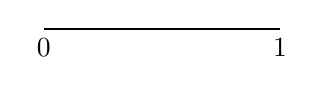
\begin{tikzpicture}
\draw[thick] (0,0)--(3,0);
\node[below] at (0,0){$0$};
\node[below] at (3,0){$1$};
\end{tikzpicture}
\end{adjustbox}
\end{center}
— такая структура $\exists$ оператор.
\begin{equation*}
(Vf)(x)=\int_0^x f(y)\,dy
\end{equation*}
(отв. в 50-х годах).
Гипотеза. Мера на прямой $\mu$.
\begin{center}
\begin{adjustbox}{max width=\linewidth}
\begin{tikzpicture}
\draw (0,0)--(4,0);
\node[below] at (0,0){$-\infty$};
\node[below] at (4,0){$+\infty$};
\end{tikzpicture}
\end{adjustbox}
\end{center}
\begin{equation*}
\mu(x)=1,\qquad L^2(\mu).
\end{equation*}
[Сверху над первым аргументом: $(x)$.]
\Unclear{GELFAND-P000088}{measure-normalization}{Видна запись $\mu(x)=1$ и ещё $(x)$ сверху; $\mu$ / $M$, значение аргумента не расширено до всей прямой.}
\begin{equation*}
(Af)(x)=\int_0^x f(y)\,d\mu(y).
\end{equation*}
\Unclear{GELFAND-P000088}{integral-origin}{Нижний предел виден как $0$, хотя строка выше говорит о мере на прямой.}
Возможно, структ. по инв. подпр. изоморфна $\operatorname{supp}\mu$.

\SourcePage{GELFAND-P000089}{61}
\underline{Возможный контрпример.}
$X$ — пр-во с мерой $\mu$.
$T$ — преобр., сохр. меру (по русски дин. система).
$\varphi$ — огр. ф-я.
[Зачёркнуто перед формулой:
\Unclear{GELFAND-P000089}{operator-cancel}{Опер. / неразборчиво}.]
[Над формулой: в $L^2$.]
\begin{equation*}
(Af)(x)=\varphi(x)f(Tx).
\end{equation*}
$\exists$ примеры преобр. с простым непр. спектром.
\begin{center}
\begin{adjustbox}{max width=\linewidth}
\begin{tikzpicture}
\draw (0,0)--(3,0);
\draw (0,-0.12)--(0,0.12);
\draw (3,-0.12)--(3,0.12);
\node[below] at (0,0){$0$};
\node[below] at (3,0){$1$};
\end{tikzpicture}
\end{adjustbox}
\end{center}
\begin{gather*}
Tx=x+\alpha\pmod1,\qquad\alpha\text{ — иррац.}\\
\varphi(x)=x.
\end{gather*}
[Справа, двойная вертикальная черта и волнистое подчёркивание:
Изучить подробно этот оператор.]
Предположение:
[Зачёркнуто:
\Unclear{GELFAND-P000089}{conjecture-cancel}{на один… / на дан… / неразборчиво}.]
нет инв. подпр. ($\forall$ вектор циклич.).
На самом деле неизв. ни одного циклич. вектора.
$\exists$ пример. опер. $A$ в $L^2(0,1)$ (Ornstein), близкий к
опер. без инв. подпр.
$\forall$ вектор $\in L^{2+\varepsilon}$ циклический (!).
(Преобр., для к-ро лебег. мера квазиинв. — мера $0$ в меру $0$ —
но инв. меры не существует.)
\begin{center}— $\bullet$ —\end{center}
\underline{Вопр. Гельфанда}: зачем нужны инв. подпр-ва и чем их можно заменить?
\begin{center}— $\bullet$ —\end{center}
Ещё один профессор, говорящий по английски (на F)
(венгр из Румынии), типа
\Unclear{GELFAND-P000089}{surname-f}{Фойтш / Фойши}
[Густо переписана повторная запись:
\Unclear{GELFAND-P000089}{surname-cancel}{ойши / Фойши / неразборчиво}.]
\begin{gather*}
E,\qquad|\lambda|<1,\qquad H(\lambda):E\longrightarrow E_*,\\
\|H(\lambda)\|\leq1.
\end{gather*}
[Буква $H$ в первой записи обведена.]
Аналит. в сильной опер. топ. (аналит. сжатие).
\begin{equation*}
\{E,E_*,H\}
\end{equation*}
[Последняя буква в тройке обведена.]
\Unclear{GELFAND-P000089}{tuple-letter}{В тройке обведённый знак: $H$ / $\Theta$ / неразборчиво; выше обведённое $H$ имеет два ясных вертикальных штриха.}
Пр-во ф-й со знач. в исх. гильб. пр-ве $E$.
$L^2(E)$ — $L^2$ на окр. $2\pi$.
\begin{equation*}
H^2(E)\qquad\int_0 u(t)e^{int}\,dt=0,\qquad n=1,2,3,\ldots
\end{equation*}
\Unclear{GELFAND-P000089}{fourier-bound}{У интеграла ясно написан нижний $0$, верхний предел отдельно не виден.}
(граничные к аналит. ф-ям).
Не всё сделано в неконечномерном случае.
Инвар. дифф. преобр. $A:H_1\longrightarrow H_2$,
$H_1,H_2$ — конечномерны.
($H\to H$ — жорданова форма.)
Разные аналоги жорд. клеток.
\begin{equation*}
\int_0^x f(x)\,dx.
\end{equation*}

\SourcePage{GELFAND-P000090}{unlabelled}
20/IX.
\underline{Kohn.}\quad $\bar\partial$ — пробл. Неймана.
[Слева $M$ в кружке.]
\begin{equation*}
M\subset C^n\qquad\text{огр. обл.}
\end{equation*}
\Unclear{GELFAND-P000090}{complex-dimension}{Показатель над $C$ густой: $n$ / $m$.}
\begin{equation*}
u_{\bar z_j}=\frac12(u_{x_j}+iu_{y_j})=\alpha_j.
\end{equation*}
Даны $\alpha_j$, когда $\exists u$ и как оно зависит от $\alpha$.
Связь с класс. теорем.
\begin{gather*}
\bar\partial u=\alpha,\\
\sum u_{z_j}\,d\bar z_j=\sum\alpha_j\,d\bar z_j\\
\text{при усл. }\alpha_{j\bar z_k}=\alpha_{k\bar z_j}\qquad(\bar\partial\alpha=0).
\end{gather*}
\Unclear{GELFAND-P000090}{derivative-convention}{В сумме индекс $z_j$ без уверенно видимой черты; выше в определении ясно $\bar z_j$.}
\underline{Проблема Леви.}
Дано $p\in\partial M$ (гран.),
[Зачёркнуто:
\Unclear{GELFAND-P000090}{levi-problem-cancel}{какая / неразборчиво}.]
$\exists$ голом. ф-я в $M$, к-рая не продолж. за точку $p$? Сущ.
Классич. теор. Леви реш. эту прбл. локально:
$r$ — ур-е границы.
\SourceFigure{GELFAND-P000090}{boundary-signs}{Слева замкнутая неровная кривая, $-$ внутри и $+$ снаружи сверху справа. Справа под буквой $r$ стоят $x$ и $0$ друг под другом; их точная роль неясна.}
\begin{equation*}
dr\neq0
\end{equation*}
(точка неособая).
В т. $p\in\partial M$
\begin{equation*}
\sum r_{z_i}(p)a^i=0\qquad\text{гиперпл.}
\end{equation*}
\begin{equation*}
\sum r_{z_i\bar z_j}(p)a^i\bar a^j
\end{equation*}
— форма Леви.
\Unclear{GELFAND-P000090}{boundary-notation}{Буква функции границы похожа на $r$ / $\tau$, знак границы на $\partial$ / $b$.}
Если она полож. опр. на указ. гиперплоскости,
то сущ. в окр. т. $p$
[Зачёркнуто:
\Unclear{GELFAND-P000090}{local-cancel}{неразборчиво}.]
ф-я, не прод. за точку $p$.
($\exists$ полином $W$, такой что нули расп. так:
\SourceFigure{GELFAND-P000090}{local-w-geometry}{Замкнутая неровная кривая слева от почти вертикальной линии; у пересечения подпись $p$, справа горизонтальный уходящий штрих. Детали пересечения и нулевого множества не восстановлены.})
Хороший ответ на ту зад. ($\bar\partial$) прив. к глоб. реш. пробл. Леви.
Пусть $\bar\partial$-прбл. разрешима для обл. $M$
($\forall\alpha$, $\bar\partial\alpha=0$, $\exists u$, $\bar\partial u=\alpha$).
Пусть
\begin{equation*}
g=\begin{cases}1&\text{в окр. }p,\\0&\text{вне }U\end{cases}
\end{equation*}
— срез. ф-я.
Обозн. $\alpha=\bar\partial\left(\frac gW\right)$.
$W$ — ранее постр. многочлен.
$\alpha$ — гладкая вплоть до границы.
\SourceFigure{GELFAND-P000090}{cutoff-geometry}{Слева три вложенных неровных контура, через них наклонная линия; подпись $p$ у малого внутреннего контура. Отношение контуров к границе и $U$ не подписано явно.}
Решим ур-е к-л., получим $u$, рассм. $h=u-\frac gW$.
$h$ голом. (т. к. $\bar\partial=0$)
[Зачёркнут штрих:
\Unclear{GELFAND-P000090}{final-arrow-cancel}{стрелка / неразборчиво}.]
$u$ не продолжается.
\Unclear{GELFAND-P000090}{noncontinuation-letter}{Перед «не продолжается» видна буква $u$, хотя непосредственно перед ней определено $h$.}
\Unclear{GELFAND-P000090}{analogo-word}{Аналого / Аналогично}
тоже можно, но там за точку продолж.
\SourceFigure{GELFAND-P000090}{global-geometry}{Нижний левый рисунок: внешний контур, внутренний контур с выемкой внизу, штриховка между ними; малый овал у выемки и несколько длинных штрихов со стрелками вниз. У правой кромки рисунка зачёркнуто слово.}
[Зачёркнуто справа от рисунка:
\Unclear{GELFAND-P000090}{figure-cancel}{неразборчиво}.]
Нужно учт. геом. структуру в целом всей области.
\SourcePage{GELFAND-P000091}{62}
$a^{p,q}$ — пр-во форм типа $p,q$.
\begin{equation*}
a^{p,q-1}\overset{\bar\partial}{\longrightarrow}
a^{p,q}\overset{\bar\partial}{\longrightarrow}a^{p,q+1}.
\end{equation*}
[Под первой стрелкой обведено: «ур-е».]
\Unclear{GELFAND-P000091}{forms-space-letter}{В начале и цепочке буква $a$ / $\alpha$; ниже похожая буква $\alpha^{p,q}$. Облик оставлен по месту.}
Общие теоремы. $\alpha^{p,q}$ — гильб. скал. произв.
$\varphi,\psi\in D_{\bar\partial^*}$.
\begin{equation*}
Q(\varphi,\psi)=(\bar\partial\varphi,\bar\partial\psi)
+(\bar\partial^*\varphi,\bar\partial^*\psi).
\end{equation*}
[Справа:] ($\bar\partial$ на гладк. формах 1-й степ. без гр. условий).
[Обведено тремя сторонами:]
\begin{equation*}
\bar\partial^*\bar\partial\varphi+\bar\partial\bar\partial^*\varphi=\alpha.
\end{equation*}
С пом. полож. опр. зад.
\Unclear{GELFAND-P000091}{positive-problem-cancel}{После «зад.» густо зачёркнуто прежнее краткое выражение; видны начальный 1-/4-подобный штрих и конечная черта.}
большого пор. реш. зад. 1-го пор.
Но здесь исп., что сист. 1-го пор. и усл. разреш. 1-го пор.
(По общ. переопр. сист. $\exists$ раб. Спенсера.)
Связ. с нейман. зад.
Апр. оц.
\begin{equation*}
\int_{\partial M}|\varphi|^2\,dS\le C Q(\varphi,\varphi)
\qquad\forall\varphi\in D_{\bar\partial^*}\cap\alpha^{p,q}.
\end{equation*}
(но не макс. $\sum$ кв. 1-х произв., $n=1\sim\int$ Дирихле).
Попытка прим. проекции (лок.) нет, ни к чему не прив.
(Cohn 2 года зан. этим, $\int$ ур-я и т. д.)
Простейший случай нейман. задачи.
Cohn и Rossi Ann. Math. 1965 о голом. продолж. форм (!) внутрь обл.

\underline{Планы на будущее.} \Unclear{GELFAND-P000091}{plans-title-correction}{Слово «на» в заголовке густо переписано; прежние штрихи не отделены.}
\underline{Учить:} Винберг (алгебраические группы),
\Unclear{GELFAND-P000091}{atiyah-parenthesis}{Атийя / Атий (в скобках густая правка перед читаемым «…дробно»), алгебр. геометрия.}
читать в порядке ликбеза:
\Unclear{GELFAND-P000091}{cancelled-book-name}{Густо зачёркнуто имя, начало $G$ / «Г…»; далее «и Rossi».}
«ф-и многих компл. пер.» 1965
(пучки, когом. и т. п.).
Обзор Дьёдонне о раб. Гротендика
\Unclear{GELFAND-P000091}{review-volume}{(Ман. 9:1 / Мат. 9:1), сокращённое первое слово не вполне уверенное.}

\underline{27/IX. Finn.} Идеи в теор. Гаусса-Бонне.
Обобщ. Кон-Фоссена: пов. не замкнутая, а полная (напр., параболоид).
\Unclear{GELFAND-P000091}{finn-curvature-cancel}{$C=2\pi$ с густо зачёркнутым последующим знаком; рядом $\chi=1$. Ниже читаемая новая запись $C=2\pi\chi$.}
\SourceFigure{GELFAND-P000091}{finn-sections}{Две открытые вверх U-образные линии. У маленькой слева почти вертикальные края и короткая поперечная стрелка внутри; справа $C=2\pi\chi$. У большой справа нет поперечной линии, подпись $\chi=1$, ниже «для неё $C<2\pi$». Точная роль внутреннего короткого штриха не установлена.}
$C=\int K\,dS$.
Теор. Кон-Фоссена: $\forall$ полн. пов. $C\le2\pi\chi$.

\SourcePage{GELFAND-P000092}{unlabelled}
Цель раб. — заменить нер-во равенством.
В след. раз обзор Волпина по вар., анал. рассл.
\Unclear{GELFAND-P000092}{next-review-name}{Последняя латинская запись $Kohn$'ом / $Kohn$'on; начало и окончание густые.}
\underline{Гельфанд.}
\Unclear{GELFAND-P000092}{atiyah-heading-cancel}{Зачёркнуто прежнее «Atiy…», затем подчёркнуто «Atiyah».}
\underline{Теоремы о неподвижных точках.}
(об. теор. Брауэра, ф-лу Лефшица, теор. о том, что лин. пр. им. соб. вектор,
теор. Вейля о следах предст. и т. п.)
$X$ — дифф. многообр. и на нём $n$ вект. рассл. $E_1,\ldots,E_n$.
$\Gamma(E_i)$ — сечения $E_i$. (кажд. рассл. — свою разм.)
\underline{Пример:} $X\times I$ ($I$ — прямая). Пр-во функций.
\underline{Эллиптический комплекс} (обобщ. элл. дифф. операторы).
\begin{equation*}
\Gamma(E_1)\overset d\longrightarrow\Gamma(E_2)\overset d\longrightarrow
\cdots\overset d\longrightarrow\Gamma(E_n).
\end{equation*}
послед. линейных отображений, таких, что $1^\circ\ d^2=0$.
$2^\circ$. Рассм. $e\in E_{i,x_0}$, $s(x)\in\Gamma(E_i)$, что $s(x_0)=e$.
Пусть $f(x)$ — функция, обращ. в $0$ в точке $x_0$.
Рассм. $d(f^m s(x))=s_1(x)\in\Gamma(E_{i+1})$.
\Unclear{GELFAND-P000092}{m-condition-cancel}{После «Тогда, если» зачёркнуто прежнее $\exists\ldots$, затем новое $\exists m$.}
что $\forall x_0$ ($f(x_0)=0$) $s_1(x_0)$ зависит лишь от 1-х дифференциалов $f$
в точке $x_0$, то опер. наз. диффер.
($\exists m$, что $\forall f$, $\forall x_0$, $\forall s$ и т. д.)
наименьшее $m$ наз. порядком дифф. опер. что $s(x_0)=e$.
(В опр. точки это лок. дифф. оператор.)
\begin{equation*}df=(\eta,dx).\end{equation*}
\Unclear{GELFAND-P000092}{gradient-corrections}{$df$ — [зачёркнуто краткое слово] вект.; $\eta$ — градиент (из «кас.» пр-ва, слово «кас.» переписано / вставлено выше).}
$\eta\in T_x^*$.
\begin{equation*}\sigma(d,\eta)e\end{equation*}
\Unclear{GELFAND-P000092}{symbol-operator-cancel}{В первом аргументе $\sigma$ густо отменён знак, над ним дописано $d$.}
— лин. ф-я $e$, наз. символом дифф. опер.
\underline{Пример.} Опр. Лапл. $m=2$.
\begin{equation*}
\frac{\partial^2(f^2(x)s(x))}{\partial x^2}
=2\left(\frac{\partial f}{\partial x}\right)^2s(x).
\end{equation*}
Символ $2(\eta_1^2+\eta_2^2+\cdots+\eta_n^2)$.
Рассм.
\begin{equation*}
0\longrightarrow E_{1,x_0}\overset{\sigma(\eta,d)}{\longrightarrow}E_{2,x_0}
\overset{\sigma(\eta,d)}{\longrightarrow}\cdots\longrightarrow E_{n,x_0}\longrightarrow0.
\end{equation*}
Комплекс эллиптический, если $\forall\eta\ne0$ эта послед. точна.

\SourcePage{GELFAND-P000093}{63}
\underline{Примеры.} $1)$ $X$ — обл. в $R^n$.
пучок $1$ ($X\times R$).
\begin{equation*}-\Gamma(1)\overset\Delta\longrightarrow\Gamma(1).\end{equation*}
опр. Лапласа.
\Unclear{GELFAND-P000093}{first-example-minus}{Перед первой $\Gamma(1)$ виден короткий минус / тире; не превращён в отсутствующий $0$.}
$2)$ комплекс де Рама.
\begin{equation*}T^*\wedge T^*\wedge\cdots\wedge T^*=\Lambda^k.\end{equation*}
\Unclear{GELFAND-P000093}{exterior-power}{При правой $\Lambda$ маленький показатель $k$ / $n$ / $x$-подобный знак; сама $\Lambda$ густо написана.}
\Unclear{GELFAND-P000093}{tangent-word-cancel}{$T$ — [начало краткого слова густо исправлено] кас. пр-во.}
$X$ — многообр. $T_x$ — кас. пр-во в точке $x$. \Unclear{GELFAND-P000093}{tangent-side-cancel}{Справа рядом с определением кас. пр-ва густо отменённая компактная запись с Т-/Ф-подобными штрихами.}
\begin{equation*}
\Gamma(\Lambda^0)\overset d\longrightarrow\Gamma(\Lambda^1)
\overset d\longrightarrow\cdots\overset d\longrightarrow\Gamma(\Lambda^n).
\end{equation*}
\Unclear{GELFAND-P000093}{de-rham-chain-cancels}{Перед $\Gamma(\Lambda^0)$ густо зачёркнуты знаки; после $\Gamma(\Lambda^n)$ зачёркнута стрелка и $0$-подобный знак.}
[Справа:] сеч. — дифф. формы.
Символ на 1-м шагу — $(\eta_1,\ldots,\eta_n)$.
\begin{equation*}d(s(x)f(x))=s(x_0)\eta=e\eta\qquad(df(x_0)=\eta).\end{equation*}
В 2-м месте
\begin{equation*}
d(s(x)f(x))\big|_{x=x_0}
=s(x)\wedge df(x)\big|_{x=x_0}=e\wedge\eta.
\end{equation*}
(каждый символ дальше — умножение на $\eta$).
\underline{Точность:} если $e\wedge\eta=0$, то $e=a\wedge\eta$.
\Unclear{GELFAND-P000093}{nilpotent-ending-cancel}{(миноры 2-го пор. $=0$, тогда векторы прям. [густо зачёркнутые заключительные знаки]); окончание не прочитано.}
$3)$ $\bar\partial$ и т. д.

\underline{4/X. Продолжение.} $\Gamma(E)$ — послед.
\begin{equation*}
d(f^m(x)s(x))\big|_{x_0}=\sigma(d,\eta)e,\qquad s(x_0)=e.
\end{equation*}
$\eta$ — 1-й дифференциал $f$.
$\eta\in T_{x_0}^*$.
Элл. опер. быв. не только диффер.
\Unclear{GELFAND-P000093}{endomorphism-heading-cancel}{Перед новым подчёркнутым «Эндоморфизм комплекса» густо зачёркнуто краткое слово, конечный штрих нисходит.}
\underline{Эндоморфизм комплекса.}
\begin{equation*}
\Gamma(E_1)\longrightarrow\Gamma(E_2)\longrightarrow\cdots\longrightarrow\Gamma(E_n).
\end{equation*}
Оно индуцирует
\Unclear{GELFAND-P000093}{induced-map-cancel}{Перед «отобр.» густо отменён короткий знак / слово.}
отобр.:
\begin{equation*}T_i^*:H^i(E)\longrightarrow H^i(E).\end{equation*}
[Справа:] $T$ — эндом. комплекса,
$T_i:\Gamma(E_i)\to\Gamma(E_i)$, коммут. с $d$.
$(T_{i+1}d=dT_i)$.
Для элл. комплекса все они конечномерн.
(В случае элл. опер. оно им. разн. индекса.)
В де Рамовом комплексе это обычные когом. с вещ. коэфф.
\begin{equation*}
L(T,E)=\sum_{i=1}^{n}(-1)^i\operatorname{tr}(T_i^*).
\end{equation*}
[Под $L$:] число Лефшица гомологич.
[Справа со стрелкой вниз:] для де-рам. компл. это обычное число Лефшица.
[Внизу:] Лефшица-Атия-Ботта.

\SourcePage{GELFAND-P000094}{unlabelled}
Пусть $f:X\longrightarrow X$.
Рассм. $\psi_i:\Gamma(f^{-1}(E_i))\to\Gamma(E_i)$.
\Unclear{GELFAND-P000094}{lifting-cancellations}{«поднятие» — [зачёркнуто «по отобр. пучков»] $f$ по отобр. пучков; в повторной записи перед $\Gamma(f^{-1}E_i)$ отменён короткий знак.}
\begin{equation*}
\psi_i:\Gamma(f^{-1}E_i)\longrightarrow\Gamma(E_i),\qquad
E_{i,f^{-1}x}\overset{\psi_{i,x}}{\longrightarrow}E_{i,x}.
\end{equation*}
\Unclear{GELFAND-P000094}{inverse-fibre-locator}{В нижнем индексе левого слоя видимое $f^{-1}x$; не заменено на $f(x)$.}
Оно неоднозначн. опред. по $f$.
Пучок де Рама: $f$ индуц. отобр. де Рам. пучков однозначно.
(естеств. поднятие).
[В рамке:] $f:X\to X$.
Предполаг., что $f$ имеет лишь конечн. число изолир. неподв. точек
самой простой структуры.
Теор. Брауэра для отрезка $[0,1]$. $f:x\to f(x)$.
\SourceFigure{GELFAND-P000094}{brouwer-graph}{Прямоугольник с нижними концами, подписанными $0$ и $1$. Внутри диагональная прямая снизу слева вверх вправо и более пологая неровная возрастающая линия; место их пересечения густое. От рисунка идёт угловая рамка под дальнейшим текстом. Точное положение пересечения не восстанавливается.}
$\rho$ — неподв. точка этого отображения.
В ней у нас есть $\psi_i(\rho):E_{i,\rho}\to E_{i,\rho}$.
\Unclear{GELFAND-P000094}{fixed-fibre-corrections}{Перед новым $E_{i,\rho}$ зачёркнута прежняя запись слоя; при «кас. пр-ве» вписано сверху $(x)$-подобное уточнение.}
В кас. пр-ве есть лин. преобразование.
Оно обозначается $J_\rho(f)$ в кас. пр-ве к $X$.
Точка изолирована $\Leftarrow$ достаточно, чтобы было
$\det(1-J_\rho(f))\ne0$ (по теор. о неявных ф-ях).
\Unclear{GELFAND-P000094}{regular-point-cancel}{После «Точка» отменено короткое слово; дальше «особая неподв., если он $0$, прав., если $\ne0$».}
Графики $(x,f(x))$ и $(x,x)$ пересек. трансверсально.
Посмотрим число
\begin{equation*}
\frac{\operatorname{tr}\psi_i(\rho)}{|\det(1-J_\rho(f))|}.
\end{equation*}
В т. $\rho$ есть 2 лин. преобр. $\psi_i(\rho)$ — слой в себя,
и преобр. кас. пр-ва.
\begin{equation*}
\sum(-1)^i\frac{\operatorname{tr}\psi_i(\rho)}{|\det(1-J_\rho(f))|}
=\sigma(\rho).
\end{equation*}
Это число не зависит от комплекса, а зав. только от $f$ и индуц. отобр. в слоях
(но отобр. слоёв не произв., оно должно коммутировать с компл.).
$\psi_i$ должно быть эндоморфизмом!

\SourcePage{GELFAND-P000095}{64}
\underline{Теорема Атия-Ботта.}
Пусть есть эллипт. комплекс $d$, $f:X\to X$ и поднятие его $\psi$,
являющееся эндоморфизмом этого комплекса. Тогда имеет место ф-ла
\begin{equation*}L(T,E)=\sum_\rho\sigma(\rho)\end{equation*}
по всем неподв. точкам.
$T$ задаётся парой $f$ и $\psi$.
\underline{Доказательство.}
\Unclear{GELFAND-P000095}{proof-opening-word}{Сначала «нечётко» / «неточно» и неполно (идеи); средние штрихи первого слова неуверенные.}
$d:\Gamma(E)_i\to\Gamma(E)_{i+1}$, по нему стр. новый оператор.
Введём в $\Gamma(E)$ скалярное произведение.
Введём «опер. Лапласа»
\begin{equation*}\Box=d^*d+dd^*.\end{equation*}
Каждое $\Gamma(E)$ перев. в себя.
Теорема Ходжа (обобщённая): $\Box$ им. дискр. положит. спектр,
каждому соб. числу соотв. кон. число соб. знач.
$\Gamma_\lambda(E_i)$ — подпр-во, ответ. соб. знач. $\lambda$ (соб. ф-и).
\begin{equation*}d:\Gamma_\lambda(E_i)\longrightarrow\Gamma_\lambda(E_{i+1}).\end{equation*}
[В овале:] $\Box d=d\Box$.
\begin{equation*}
d:\Gamma(E_1)\longrightarrow\Gamma(E_2)\longrightarrow\cdots\longrightarrow\Gamma(E_n).
\end{equation*}
Посмотрим теперь
\begin{equation*}
d:\Gamma_\lambda(E_1)\longrightarrow\Gamma_\lambda(E_2)
\longrightarrow\cdots\longrightarrow\Gamma_\lambda(E_n).
\end{equation*}
$\Gamma_\lambda$ уже конечномерны ($d^2=0$), тоже возникают гомологии.
\begin{equation*}
H^i\{\Gamma_\lambda(E)\}=
\begin{cases}
H^i(E),&\lambda=0,\\
0,&\lambda\ne0.
\end{cases}
\end{equation*}
\Unclear{GELFAND-P000095}{index-operator-abbreviation}{(индексы есть только для «дефин.» / «диффин.» опер.); сокращение оставлено неразвёрнутым.}
Для де Рам. компл. — теор. Ходжа — всякая
\Unclear{GELFAND-P000095}{harmonic-form-cancels}{После «всякая» и перед «замкн.» густо зачёркнуты два прежних выражения.}
замкн. форма гомологична гармонической.
Считать след: $\sum$ диаг. элем. $=\sum$ соб. знач.
(1. След как $\int K(x,x)\,dx$, и $\sum$ следов в каждом подпр-ве
(инв. собств.).
\Unclear{GELFAND-P000095}{nonzero-trace-cancel}{$\lambda\ne0$ [густо зачёркнут короткий знак] следа нет, $\lambda=0$ счит. через гомологии.)}

\SourcePage{GELFAND-P000096}{unlabelled}
\underline{11/X. План семинара.}
1. Интегро-дифф. операторы (Агранович). [Под скобкой:] (2 засед.)
2. Атия-Зингер по индексу. Кириллов или Гельфанд. Дынин.
(год. сем. Cartan-Schwartz и сем. Вишика 64–65).
3. Статистическая физика (Минлос, 3 засед.).
\Unclear{GELFAND-P000096}{minlos-patronymic}{Под Минлос: «Роберт Адльфович» / «Роберт Адольфович»; малая петля после «д» не вполне установлена.}
4. Адели и группы аделей (Граев Марк Иосифович). (2 засед.)
\Unclear{GELFAND-P000096}{graev-initial-cancel}{Между «Граев» и «Марк» густо зачёркнут М-подобный прежний знак.}
5. Линейные алгебраические группы. [Справа столбиком:] Кириллов; Гельфанд.
6. Работа Ботта и Chern (Acta Math.). Гельфанд.
\Unclear{GELFAND-P000096}{chern-volume-correction}{Под названием журнала «Т. 114» / «Т. III», $N=1$–$2$, цифры густые; ниже отменён короткий знак перед «кривые».}
(перенес. теор. Неванлинны о нулях ф-й на кривые сеч. вект. пучков).
7. Теорема Римана-Роха-Гротендика. Каздан Д. А.

\underline{Каздан.} Теор. Римана-Роха.
Вект. пучку соотв. класс когом. — класс Chern'а.
\underline{Классы Черна.}
$X$ — классич. алг. многообразие, афф. пр-во.
Алг. ф-ии на нём — многочлены, это самое простое алг. многообразие.
Аффинные алг. многообр. Пусть дан набор многочленов
$p_1(x_1,\ldots,x_n),\ldots,p_k(x_1,\ldots,x_n)$.
(пусть поле $k$ — алг. замкнуто).
Рассм. наборы точек — удовл. ур-ю, афф. алг. мн-…
— алг. ф-ии — ограничения многочленов —
— факторкольцо по идеалу, натян. на мног.
Алг. предмногообр. — пр-во, лок. изоморфное афф. многообр.

\SourcePage{GELFAND-P000097}{65}
Если доб. условия $Q_1(x_1,\ldots,x_n)\ne0$,
$Q_i(x_1,\ldots,x_n)\ne0$, (все сразу $\ne0$),
\Unclear{GELFAND-P000097}{nonzero-top-cancel}{Справа сверху густо зачёркнуты две строки прежней записи; отдельные горизонтальные и петлеобразные штрихи не дают надёжного чтения.}
то тоже алг. мн-зе.
ф-и — из рац. ф-ий с полюсами вне этих точек.
\underline{Пример:} прямая, алг. ф-и — многочлены.
Пр-во зад. с запасом ф-ий.
Рассм. точки $x\ne0$. ф-и уже $\frac{P(x)}{x^m}$.
Афф. мн. — нули нек-рых ф-ий и другие не обр. в $0$.
\underline{Общее алг. мн.:} $\forall$ точки сущ. откр. окр.,
изоморфная афф. алг. многообр.
(сначала только дифф. мн. или окольцов. пр-во).
Окольц. пр-во —
\Unclear{GELFAND-P000097}{ringed-space-cancel}{Между тире и «мн-зе» густо отменён короткий знак / слово.}
мн-зе с пучком колец. [Под «мн-зе» вставлено: «(пр-во)».]
Каждое афф. алг. мн-зе — окольцов. пр-во.
На нём ввод. топ. Зарисского.
(Чтобы все алг. ф-и были непр. — замкн. мн-ва —
нули конечного числа алгебр. ф-ий).
Пучок колец — откр. мн-во в нём это тоже алг. многообразие.
\Unclear{GELFAND-P000097}{left-margin-traces}{В левом поле рядом со следующими строками слабые серые следы записей и густой А-подобный знак; надёжных цельных слов не прочитано.}
$C^2\setminus0$ не афф. алг. многообр.
[Над следующей строкой приписано со скобкой: «откр. мн-во».]
Каждое афф. алг. многообразие
\Unclear{GELFAND-P000097}{open-variety-cancel}{«содер…»: окончание слова густо перечёркнуто.}
откр. подмн-во, явл. алг. многообр.
\underline{Пучок}
\Unclear{GELFAND-P000097}{sheaf-prefix-mark}{Перед «колец» отдельно н-/и-подобный густой знак, его роль не установлена.}
колец — надо опр. группу сечений
на базисных откр. мн-вах получ. ур-ями вида $R_1(x)\ne0$,
кольцо алгебр. ф-ий на этом мн-ве.
Получ. пучок ростков алг. ф-ий, окольцов. пр-во.
Окольц. пр-во — предмн. мн-зе, если оно
лок. изоморфно афф. алг. мн-зю. (как окольц. пр-во)

\SourcePage{GELFAND-P000098}{unlabelled}
Афф. алг. мн.
[Слева под фигурной скобкой:] $p_1=$; $\ldots$; $p_m=0$; ниже $Q\ne0$.
\Unclear{GELFAND-P000098}{affine-opening-cancel}{После $p_1=$ правая часть не видна; справа перед «замкн. мн-во» густо отменена прежняя краткая запись.}
замкн. мн-во.
$R_i(x_1,\ldots,x_n)=0$. $R_i$ — многочлены.
База откр. мн-в — одно условие $U_S:S\ne0$.
(такое сод. во всяком откр. — оставим $1$ условие).
Группа сечений зад. так —
$\Gamma(U_S)$ — все рац. ф-и на $R^n$, не обр. в $\infty$
нигде на нашем мн-ве.
\begin{equation*}\Gamma(U_S)=\left\{\frac{P(x)}{Q(x)}\right\}.\end{equation*}
\Unclear{GELFAND-P000098}{sections-relation-overwrite}{Между $\Gamma(U_S)$ и фигурной скобкой две горизонтальные черты с густой правкой между ними; знак переписан, диагональная черта не установлена.}
Отожд., если на $U_S$ одно значение.
Это кольцо.
(Это будет пучок, легко док., что это действ. будет гр. сечений.)
Изом. пучков получ. определением изоморфизма
\Unclear{GELFAND-P000098}{isomorphism-base-word}{Последнее сокращение верхней строки «баз.» / «без.»; следующей строкой: «гомеом. ест.»}
\SourceFigure{GELFAND-P000098}{sheaf-isomorphism-diagram}{Верхний ряд $E$ и $E'$, соединённые двусторонней горизонтальной стрелкой; от каждого вниз толстая стрелка к $B$, соответственно $B'$. В нижнем ряду горизонтальная стрелка не видна. Толстые верхние концы не позволяют уточнить очертание наконечников.}
Если $E$ — подпучок ф-ий, то
$B\longrightarrow B'$ индуцирует $E'\longrightarrow E$.
(A priori только коммут.) Треб., чтобы изом.
был изом., возникн. из сообр. базы. (естеств.!) просто совпадение!
$C^2\setminus0$ это предалг. мн-зе.
Выбр. $2$
\Unclear{GELFAND-P000098}{two-lines-word}{«прямые» / «прямки»: средние и конечные штрихи тесные.}
$1$-е на $x\ne0$, $2$-е $y\ne0$.
\SourceFigure{GELFAND-P000098}{punctured-plane-diagram}{В прямоугольной рамке вертикальная и горизонтальная толстые линии пересекаются посередине. Правая и нижняя оконечности утолщены, левый конец заострён; точная роль утолщений / стрелок не установлена. Буквенных подписей нет.}
Наше мн-во — их объедин. Каждое из них афф. мн-зе.
Затем соглас. пучки колец уже ясно.
Точки [Вставлено сверху: «пред».] алг. мн-зий могут быть неразделимы для ф-ий.
\underline{Пример пр. афф. [Вставлено сверху со скобкой: «пред».] алг. мн-зий.}
\begin{align*}
p_1(x_1,\ldots,x_n)&=0,\\
p_k(x_1,\ldots,x_n)&=0,\\
Q(x_1,\ldots,x_n)&\ne0.
\end{align*}
\Unclear{GELFAND-P000098}{last-coordinate-indices}{Последние нижние индексы аргументов густые: $x_n$ / $x_m$; во второй строке над последним индексом есть ещё короткий штрих.}
Последнее усл. не обязательно, любое
\Unclear{GELFAND-P000098}{affine-condition-cancels}{После «любое» густо отменено слово; ниже после «этих» зачёркнуто ещё одно слово.}
афф. алг. мн. можно задать, не используя этих условиях
($\exists$ мн., ему изоморфное).

\SourcePage{GELFAND-P000099}{66}
Берём $(x,y)$ с условием
\begin{equation*}
\begin{cases}
P_i(x)=0,\\
Q(x)y-1=0.
\end{cases}
\end{equation*}
[Вверху справа:] $(x_1,\ldots,x_n,y)$.
Они изоморфны.
Пусть есть коль. $P(x)$ и идеал $I$ — первое афф. алг. мн.
$P(y)$, $J$ — $2$-е афф. алг. мн.
Их произведение — кольцо $P(x,y)$ с идеалом
\begin{equation*}\{I\otimes[P(y)]+[P(x)]\otimes J\}.\end{equation*}
\Unclear{GELFAND-P000099}{product-ideal-notation}{Буква первого идеала $I$ / $J$-подобная и в верхней строке, и в первом слагаемом; разделяющий знак $+$ / $\oplus$ густо переписан.}
\Unclear{GELFAND-P000099}{tensor-circled-symbol}{Справа обведено «2» / «?»; ниже основной изогнутой линии отдельная точка.}
(как мн-во — обычн. произв.)
Кольцо ф-ий на нём — тенз. пр. колец ф-ий на тех мн.
Пр. произв. любых предалг. мн. —
\Unclear{GELFAND-P000099}{product-and-heading-cancels}{После тире густо отменено выражение, под ним короткий угловой штрих и чёрная помета. Также перед «Заметим» ниже густо зачёркнут прежний начальный знак.}
$X,Y$ — [Сверху вставлено: «пред».] алг. многообр.
$\{U_i\}$, $\{V_j\}$ — $2$ покр. афф. откр. подмногообр.
$X\times Y$ покрыто $U_i\times V_j$. Это есть напр. мн-обр.
Заметим, что произв. мн. не есть произв. топ. пр-в
(топ. не есть топ. произв.).
Рассм. $X\times X$. Выберем в нём [Под строкой: «в нём структ.»].
\Unclear{GELFAND-P000099}{subvariety-prefix-correction}{«Предалг.» в начале определения подмногообр. густо переписано в середине.}
Предалг. подмногообр. — замкнутое подмн-во в топ. Зарисского.
Оно само предалг. мн-зе.
В $X\times X$ есть диагональ $(x,x)$.
Если она замкнута, то мн-зе наз. алгебраическим.
[Это станд. —
\Unclear{GELFAND-P000099}{presheaf-diagonal-term}{Читается «предпучок наз. пучком, если диагональ замкнута»; видимое слово «предпучок» оставлено, без замены по определению многообразия.}
Топ. в $X$ отделимая, если диаг. $X\times X$ замкнута.]
\underline{Пример} предалг., но не алг. $X$.
$(U_1,U_2)$ — покр.; $U_1,U_2$ — изом. прямой.
$U_1\cap U_2$ изом. прямой с выкол. точкой.
\SourceFigure{GELFAND-P000099}{double-origin-diagram}{Одна почти горизонтальная линия с утолщённой точкой около середины. Над точкой $x'$, под ней $x''$; обе подписи относятся к одному месту нарисованной линии. Справа толстый стрелкообразный знак перед дальнейшей фразой. Две отдельные линии не дорисованы.}
Проверить, что диаг. не замкнута.

\SourcePage{GELFAND-P000100}{unlabelled}
\underline{Классы циклов по модулю лин. экв.}
(более точный инв., чем когом.)
$X$ — алг. многообр., подмн. — замкн. мн-во в топ. Зарисского.
$V_i$ — подмногообр.
\begin{equation*}\sum a_iV_i\text{ — циклы}\qquad(a_i\text{ — целые}).\end{equation*}
[Под суммой: «форм.».]
$\sum b_iU_i$. $2$ цикла линейно экв., если
$X\times P^1$ — в нём есть подмн. $X\times a$, $X\times b$;
$a,b\in P^1$.
($P^1$ покр. двумя об. прям. — алг. мн.)
[Слева чёрный звёздочкообразный знак.]
Они кан. изом. $X$.
$2$ цикла экв., если
\Unclear{GELFAND-P000100}{cycle-equivalence-cancels}{После «если» отменено короткое выражение; ниже после «с» отменено ещё одно слово.}
$\exists$ $3$-й цикл $W\in X\times P^1$,
дающий в пересеч. с $X\times a$ первый, а с $X\times b$ второй.
\underline{Пример.} $X$ — поверхность, $U,V$ — кривые.
Они лин. экв., если $\exists$
\Unclear{GELFAND-P000100}{rational-function-cancel}{Перед «ф-я» отменён маленький густой знак с замкнутой петлёй.}
ф-я с нулями на $U$ и полюсами на $V$.
Рассм. $X\times P^1$. Берём в нём $a=0$ и $b=\infty$.
В $X\times P^1$ берём цикл $(x,f(x))$.
\underline{Опред. классов}
\Unclear{GELFAND-P000100}{chern-name-overwrite}{«Черна»: середина и конечные штрихи имени густо переписаны, прежние буквы не отделены.}
(алг. мн-зий).
Они зад. с
\Unclear{GELFAND-P000100}{axiom-abbreviation}{«кон.» / «нек.» аксиом.; краткое слово имеет тесные средние штрихи.}
\Unclear{GELFAND-P000100}{category-cancellations}{Перед «Функтор» густо отменён прежний начальный знак; после «из категории» отменён и обведён скобкой / окружностью ещё один знак.}
Функтор из категории
Алгебр. пучок, алгебр. $K$-функтор.
[Справа:] $A(X)$ — гр. лин. экв. циклов.
Отобр. $K(X)\longrightarrow A(X)$ линейное.
\underline{Аксиомы.}
\Unclear{GELFAND-P000100}{first-axiom-cancel}{Последняя строка: «1.» и густо зачёркнутое продолжение. После него новых читаемых аксиом на этом кадре нет.}




\SourcePage{GELFAND-P000101}{67}
\underline{18/X. И.М. Гельфанд.}
[Под датой отдельно: $X$.]

$E_1,\ldots,E_n$
\begin{equation*}
\Gamma(E_1)\overset{d}{\longrightarrow}\Gamma(E_2)
\overset{d}{\longrightarrow}\cdots\overset{d}{\longrightarrow}\Gamma(E_n)
\end{equation*}
[Справа зачёркнуты две записи:]
\Unclear{GELFAND-P000101}{top-cancellations}{Дифф. / Диффер.; опер. / неразборчиво}
Элл. комплекс.
\begin{equation*}
d\bigl(f^m(x)s(x)\bigr)\big|_{x_0}=\sigma(d,\eta)s(x_0),
\qquad df\big|_{x_0}=\eta
\end{equation*}
$\sigma$ — символ дифф. опер.
\begin{equation*}
0\longrightarrow E_{1,x_0}
\overset{\sigma(d,\eta)}{\longrightarrow}E_{2,x_0}
\longrightarrow\cdots\overset{\sigma(d,\eta)}{\longrightarrow}
E_{n,x_0}\longrightarrow0.
\end{equation*}
\underline{Отобр.} $T:\Gamma(E)\longrightarrow\Gamma(E)$.

$f:X\longrightarrow X$

$\varphi$ \Unclear{GELFAND-P000101}{bundle-contraction}{эндом. / индуц.} рассл.
[Справа: $\Gamma(E_i)\to\Gamma(E_i)$. Под этим зачёркнут квадрат:]
\SourceFigure{GELFAND-P000101}{cancelled-bundle-square}{Зачёркнутые верхние $E_i$ со стрелкой вправо, вертикальные стрелки вниз к $X$ и нижняя стрелка вправо; точные штрихи индексов скрыты. Рядом активный квадрат приведён ниже.}
\begin{center}
\begin{adjustbox}{max width=\linewidth}
\begin{tikzcd}
E_i \arrow[r,"\varphi"] \arrow[d] & E_i \arrow[d]\\
X \arrow[r,"f"] & X
\end{tikzcd}
\end{adjustbox}
\end{center}
(В простейш. случаях $\varphi$ определяет $f$ —
— формы $f$ опред. отобр. кас. векторов)

Эндом., если коммут. с $d$.

$T$ есть опер. в $C^\infty$-пр-ве. Теорема свод. к изуч. следа
(он счит. 2-мя способами)

\underline{Теорема 1.} Комплекс имеет конечные
[зачёркнуто:] \Unclear{GELFAND-P000101}{theorem-cancel}{размерные / неразборчиво}
гомологии.

Пусть $\omega^n$ — форма пор. $n$ на $X$, не обращ. в 0.
Введём с её помощью эрмитову структуру. (Пусть она
сущ. раз и навсегда. Неинвариантно, но проще.)
\begin{equation*}
\int\langle s,\alpha(s')\rangle
=\int_X\overline{(s,s')}\,\omega,
\qquad d^*\underset{\mathrm{def}}{=}\alpha^{-1}\cdot d'\circ\alpha.
\end{equation*}
$s\in\Gamma(E)$, $s'\in\Gamma_c(E')$.

$E'$ — сопр. пучок.
\begin{equation*}
\Box\underset{\mathrm{def}}{=}d^*d+dd^*
\end{equation*}
($d'$ — просто сопр. оператор)

$\Box$ — эллипт. оператор, перев. каждое $\Gamma(E_i)$ в себя.

$\Gamma_\lambda(E)$ — сечения, удовл. ур-ю $\Box s=\lambda s$.
Т.к. $\Box$ эллиптичен, то $\forall\lambda$ кон. число разл. лин. незав. соб. ф-й
[после ф-й густой отдельный знак:]
\Unclear{GELFAND-P000101}{eigenfunction-end-sign}{зачёркнутое $H$ / неразборчиво}.
\begin{equation*}
\Box d=d\Box
\end{equation*}
\begin{equation*}
\Gamma_\lambda(E_1)\overset{d}{\longrightarrow}\Gamma_\lambda(E_2)
\overset{d}{\longrightarrow}\cdots\longrightarrow\Gamma_\lambda(E_n)
\end{equation*}
Введём группы гомологий
[ниже зачёркнуто:] \Unclear{GELFAND-P000101}{homology-cancel}{неразборчивая формула / $H^i(\Gamma)$}
\begin{equation*}
H^i(\Gamma_\lambda(E))=\ker d\big|_{\Gamma_\lambda(E_i)}.
\end{equation*}
[Справа от последней формулы наклонная дробная черта; знаменатель зачёркнут:]
\Unclear{GELFAND-P000101}{homology-denominator}{$\operatorname{Im}\,d$ / неразборчиво}.

\SourcePage{GELFAND-P000102}{unlabelled}
Без док-ва в этой работе утв. теорема Ходжа
\begin{equation*}
H^i(\Gamma_\lambda(E)^*)=
\begin{cases}
H^i(E)&\lambda=0\\
0&\lambda\ne0.
\end{cases}
\end{equation*}
\Unclear{GELFAND-P000102}{complex-star}{Над скобкой у $\Gamma_\lambda(E)$ отдельный $*$ / след переписывания; положение относительно скобок неясно.}
\underline{Дынин.} При $\lambda\ne0$ — здесь 0.
($d$ при $\lambda\ne0$ перев. соб. ф-и
[зачёркнуто:] \Unclear{GELFAND-P000102}{dynin-cancel}{неразборчиво / соб.}
точн. компл.
\begin{equation*}
\underline{H^i(\Gamma_\lambda(E))=\ker(\Box-\lambda)},
\end{equation*}
это теор. Ходжа $\forall\lambda$
($\forall$ элл. опер.
[зачёркнуто:] \Unclear{GELFAND-P000102}{dynin-general-cancel}{неразборчивое сокращение}
[под ним: ?]
$\Box-\lambda$ — новая буква, снова теор. Ходжа\ldots ?)
\Unclear{GELFAND-P000102}{dynin-kernel-claim}{Запись $H^i(\Gamma_\lambda(E))=\ker(\Box-\lambda)$ сохранена буквально; $i$ справа не указан.}

\underline{Бернштейн.} То же.
$H^i(\Gamma_\lambda(E))=0$, $\lambda\ne0$.
Пусть $s\in\Gamma_\lambda(E_i)$ и пусть $ds=0$.
[Перед $\Box$ густо написано $d$ / скобка:]
\Unclear{GELFAND-P000102}{bernstein-square-prefix}{$d$ / открывающая скобка / след переписывания}
$\Box s=dd^*s$. Тогда $\lambda s=d(d^*s)$
и $s=d\left(\frac{d^*s}{\lambda}\right)$,
$d^*s$ есть соб. ф-я ($d^*$ коммут. с $\Box$).

$d^*s\in C^\infty$ след. из \underline{теор. об элл.} ур-ях.
\underline{Опять Гельфанд.}
При $\lambda=0$ букв. перен. док-во Ходжа.
\begin{equation*}
\Gamma(E)=\sum\Gamma_\lambda(E)\qquad(\text{дискр. спектр})
\end{equation*}
Кроме опер. $T$ введём
\begin{equation*}
\fbox{$T_\lambda=\pi_\lambda\circ T\circ i_\lambda$},
\qquad i_\lambda:\Gamma_\lambda(E)\longrightarrow\Gamma(E),
\end{equation*}
где $\pi_\lambda:\Gamma(E)\longrightarrow\Gamma_\lambda(E)$ —
проекция ортог.

(опер. $T$ в этой клетке) Число Лефшица для $T$.

$T$ — отобр. сечений, тем самым отобр. сечений
$\Gamma(E)\to\Gamma(E)$
\begin{equation*}
L(T,E)=\sum(-1)^i\operatorname{tr}(T_i^*|H_i).
\end{equation*}
\Unclear{GELFAND-P000102}{lefschetz-space}{После вертикальной черты густо переписанное $H_i$ / $H^i$ / неразборчиво.}
В силу теор. Ходжа $T_{\lambda=0}=T^*$.
[Справа отдельно:] $\pi_0=T^{**}$
\Unclear{GELFAND-P000102}{hodge-stars}{Справа $\pi_0$ / $T_0$ и один / два переписанных звёздочных штриха над $T$.}
\begin{gather*}
\sum(-1)^i\operatorname{tr}(T_0|E_i)=L(T,E)\\
\sum(-1)^i\operatorname{tr}(T_\lambda|E_i)=0\qquad\lambda\ne0
\end{gather*}
[Справа две густо зачёркнутые небольшие записи:]
\Unclear{GELFAND-P000102}{right-cancellations}{неразборчиво}.

(след в гом. всё равно, что след в самих пр-вах)

(По теор. Ходжа $H^i(E)=\Gamma_0(E_i)$)
\begin{equation*}
\Box s=0\Longrightarrow ds=0
\end{equation*}
[Стрелка густо переписана.]
(из \Unclear{GELFAND-P000102}{positive-aside}{полож. / непоср.} опр. и т.п.)

Надо придать смысл $\sum(-1)^i\operatorname{tr}(T|E_i)$.
Его регуляриз.

2-мя способами.

\SourcePage{GELFAND-P000103}{68}
В конеч. $\Gamma_\lambda(E)$
\begin{equation*}
d:\Gamma_\lambda(E_1)\longrightarrow\Gamma_\lambda(E_2)\longrightarrow\cdots
\end{equation*}
(конечномерность)
$T$ — его отобр. в себя. Тогда
\begin{equation*}
\sum(-1)^i\operatorname{tr}T|_{E_i}
=\sum(-1)^i\operatorname{tr}T|_{H_i}
\end{equation*}
(а $H^i=0$)

(инвар. эйлер. характеристики)

Рассм.
\begin{equation*}
\sum_\lambda(1+\lambda)^{-z}\operatorname{tr}(T_\lambda|E_i)
=\operatorname{tr}^{z}(E_i)
\end{equation*}
\underline{Теорема.} Ряд сх. при $\operatorname{Re}z>\frac12\dim X$
(об асимпт. соб. ф-й) (Данфорд и Шварц, т.2)

Это анал. ф-я $z$ в полупл.
\begin{equation*}
L(T,E)=\sum(-1)^i\operatorname{tr}^{z}E_i\qquad\forall z
\end{equation*}
(всё, кроме сходимости, доказано
[густо переписанный знак после слова:]
\Unclear{GELFAND-P000103}{proof-overwrite}{неразборчиво}
—
\SourceFigure{GELFAND-P000103}{proof-grid}{После тире небольшой прямоугольник с густой сеткой горизонтальных и вертикальных штрихов; его точная роль не подписана.})

Т.к. $T\sim$ ограничен (асимпт. соб. ф-й)

(при аналит. прод. при $z=0$ полюс)

\underline{Пример.} $S^1$ [окружность, справа метка $t$],
$d=\frac d{dt}$, элл. опер., $\Box=\frac{d^2}{dt^2}$.

$T=(f,\varphi)$,
\begin{gather*}
dS(x)=s(x)\\
Ts(x)=\varphi(x)s(f(x))
\end{gather*}
\SourceFigure{GELFAND-P000103}{small-wave}{Слева ниже $T=(f,\varphi)$ волнистый штрих, под ним почти горизонтальный штрих со стрелочным правым концом. Оси и функции не подписаны.}

\underline{Определение} [перед псевдодифф. густой переписанный знак:]
\Unclear{GELFAND-P000103}{definition-prefix}{неразборчиво / $P$}
псевдодифф. опер:

$X$ — многообр. $\Gamma(E)$, $\Gamma(F)$ — 2 рассл. на $X$
\begin{equation*}
P:\Gamma_c(E)\longrightarrow\Gamma(F)
\end{equation*}
$\Gamma_c(E)$ — сеч. с комп. носителем.
[Зачёркнуто:] \Unclear{GELFAND-P000103}{pseudo-cancel}{Наз. / неразборчиво}
Лин. опер. наз. псевдодифф., если $\exists$ послед. чисел
$n_1>n_2>n_3>\cdots\to-\infty$
\Unclear{GELFAND-P000103}{order-signs}{Знаки $>$ / $\geq$; средний знак густо переписан, отдельные нижние штрихи не установлены.}
и уд. след. условиям
\begin{equation*}
e^{-i\lambda g}P(e^{i\lambda g}s)
\end{equation*}
$g\in\Gamma(1)$ ($C^\infty$-ф-я),
1 — трив. пучок, $s(x)\in\Gamma_c(E)$, $dg\ne0$ на $\operatorname{supp}s$,
если есть асимпт. разлож.
[Рядом внизу короткий густой знак:]
\Unclear{GELFAND-P000103}{bottom-mark}{неразборчиво}.

\SourcePage{GELFAND-P000104}{unlabelled}
\begin{equation*}
\sim\sum_0^\infty P_j(s,g)\lambda^{n_j}
\end{equation*}
\underline{26/X Продолжение.} Элл. комплекс.
В $E_i$ — эрмитова метрика и в $X$ — интегрирование.
Вв. опер. $d^*$, $\Box=dd^*+d^*d$, $\Box d=d\Box$.

$\Box s=\lambda s$, $\Box$ самосопр. и полож., эллиптичен, $\lambda>0$.
$\Box s=0\Longrightarrow ds=0$
\begin{equation*}
d\Gamma_\lambda(E_i)\subset\Gamma_\lambda(E_{i+1})
\end{equation*}
\begin{equation*}
0\overset{d}{\longrightarrow}\Gamma(E)
\overset{d}{\longrightarrow}\Gamma(F)\overset{d}{\longrightarrow}0
\end{equation*}
$d$ — просто эллипт. оператор, $ds=0$ — ядро.
Образ $s_1=ds_*$,
\Unclear{GELFAND-P000104}{image-preimage}{$s_1=ds_*$ / $s_i=ds^*$ / неразборчивый индекс}
\underline{Гомологии:} $\ker d|_E$, $\operatorname{Coker}d|_F$.
Число Лефшица — \underline{индекс}.
\begin{equation*}
\Gamma_\lambda(E_i)\overset{d}{\longrightarrow}\Gamma_\lambda(E_{i+1})
\longrightarrow\cdots
\end{equation*}
уже конечномерн. комплекс,
его гом. $=0$ при $\lambda\ne0$ и $=H^i$
[зачёркнуто при]
\Unclear{GELFAND-P000104}{zero-cohomology-words}{самое конеч. / само конеч.}
при $\lambda=0$.

$T_i^*$ $H^i$.
$\sum(-1)^i\operatorname{tr}(T_i^*)=L(T,E)$.
Вычислить через неподв. точки.

$T$ — отобр. $X$, коммут. с $d$.
$T$ есть отобр. $\Gamma_\lambda(E_i)$.
Введём операторы $\pi_\lambda$ и $i_\lambda$:
влож. $\Gamma_\lambda$ во всё $\Gamma$ и проектир. на
[зачёркнуто:] \Unclear{GELFAND-P000104}{projection-cancel}{неразборчивая запись}
$\Gamma_\lambda(E_i)$.
\begin{equation*}
T_\lambda=\pi_\lambda\cdot T i_\lambda
\end{equation*}
(выдел. клетки, соотв. $\Gamma_\lambda$)

Коммут. ненужно, дост.
[густой знак:] \Unclear{GELFAND-P000104}{cell-cancel}{неразборчиво}
(\SourceFigure{GELFAND-P000104}{diagonal-cells}{В круглых скобках три пустых квадрата по диагонали сверху слева вниз вправо; границы касаются. Точные размеры клеток не обозначены.})
в клетках.

Тогда \fbox{$T^*=T_0$}
\begin{equation*}
0\longrightarrow\Gamma_0(E_1)\overset{d}{\longrightarrow}\Gamma_0(E_2)
\overset{d}{\longrightarrow}\cdots
\end{equation*}
все $d=0$ т.к. $\Box s=0$.

Все гомологии в $\Gamma_0$.
\begin{equation*}
\Gamma(E_i)=\Gamma_0(E_i)+\Gamma_{\lambda_1}(E_i)+\cdots
\end{equation*}
[Под вторым слагаемым и многоточием стрелки вниз к записи гомол. 0.]

В 1-й строчке
[зачёркнуто:] \Unclear{GELFAND-P000104}{first-row-cancel}{неразборчивое слово}
ядра $\Gamma_0(E_i)$
\begin{equation*}
0\longrightarrow\Gamma_0(E_1)\longrightarrow\Gamma_0(E_2)\longrightarrow
\end{equation*}
[Под двумя членами вертикальные двойные штрихи и $H^*(E)$, $H^*(E)$.]
\Unclear{GELFAND-P000104}{cohomology-overwrite}{Оба верхних знака у $H$ густо переписаны: $*$ / индекс степени.}
\underline{Замеч.} $\pi_\lambda$ коммутирует с $d$.
\begin{equation*}
\left\{
\begin{aligned}
\sum(-1)^i\operatorname{tr}(T_0^i)&=L(T,E)\\
(-1)^i\operatorname{tr}(T_\lambda^i)&=0
\end{aligned}
\right.
\end{equation*}
\Unclear{GELFAND-P000104}{last-sum-absent}{Во второй строке перед $(-1)^i$ отдельная $\sum$ не видна.}

\SourcePage{GELFAND-P000105}{69}
Если есть послед. пр-в
\begin{equation*}
0\longrightarrow A_1\overset{d}{\longrightarrow}A_2
\overset{d}{\longrightarrow}\cdots\overset{d}{\longrightarrow}A_n
\longrightarrow0,\qquad d^2=0.
\end{equation*}
и отобр. $T_i$, комм. с $d$. Тогда
\begin{equation*}
\sum(-1)^i\operatorname{tr}T_i=\sum(-1)^i\operatorname{tr}(T_i^*).
\end{equation*}

[Под левой суммой: в целых; под правой: в гомол.; справа: (ф-ла Эйлера).]
(ф-ла Эйлера получ., если взять $T=E$)

\underline{Док-во:} предст. $A_i=Z+C_Z$, $Z=B+\text{доп.}$ и потом
рассм. $T$ там.
[Под $Z$: $Z$ 3-х слаг.]
$\operatorname{tr}T_\lambda$ дост. заменить на $\operatorname{tr}T_\lambda^*$,
а [зачёркнуто:] \Unclear{GELFAND-P000105}{homology-cancel}{неразборчиво}
$H_\lambda=0$.

Введём
\begin{equation*}
\operatorname{tr}^z(E_i)=
\sum_\lambda(1+\lambda)^{-z}\operatorname{tr}(T_\lambda^*|E_i)
\end{equation*}
при $\operatorname{Re}z>\frac12\dim X$,
[Справа:] $\lambda_n\sim n^{K/\dim X}$.
\Unclear{GELFAND-P000105}{eigenvalue-power}{$K$ / $\kappa$ в числителе показателя.}
\begin{equation*}
\sum(-1)^i\operatorname{tr}^z(T_i^i)=L(T,E)\quad\text{при всех }z.
\end{equation*}
\Unclear{GELFAND-P000105}{trace-argument}{У $T$ два густых знака: $T_i^i$ / $T_i$ / неразборчивый верхний знак.}

\underline{Теорема о продолжении}
(ссылка на
\Unclear{GELFAND-P000105}{continuation-name}{Narasimhcan a / Narasimhana}
и др.)
[Над «и др.»: \Unclear{GELFAND-P000105}{continuation-side-name}{катаcэ. / катасэ. / неразборчиво}]
[Ниже: Nirenberg,
\Unclear{GELFAND-P000105}{continuation-middle-name}{Cohna / Cohn a},
Hörmander.]

$\operatorname{tr}^zT^i$ продолжима во всю плоскость, аналитична
во всей плоскости (!) и при $z=0$
\begin{equation*}
\operatorname{tr}^0(T^i)=\operatorname{tr}^b(T^i)
\end{equation*}
\Unclear{GELFAND-P000105}{trace-superscript-overwrite}{Верхний знак у второго $\operatorname{tr}$ густо переписан; $b$ / неразборчиво.}
где $\operatorname{tr}^b$ — след, счит. обычн. способом через обобщ. ф-и.

$T=E$ не годится (получ. $\zeta(s)$ с полюсами), но рассм.
опер. \Unclear{GELFAND-P000105}{operator-mark}{густой переписанный знак},
им. конечн. число неподв. точек (простых).
[Вставка под $T=E$:] $(\operatorname{tr}E=\infty\text{ при }z=0)$.

$\operatorname{tr}^b$: $T$ имеется в виде ядра, $\int\kappa(x,x)\,dx$.
$\operatorname{tr}^b$ — счит. через неподв. точки.
[Над «неподв.»: (обобщ. ф-и).]
(Вариант послед. ф-й, сход. к $\delta$-ф-и)
Некоторый вар. $b$-следа.
[Справа:] $\delta(x,a)$ — $\delta$ в точке $a$.
\begin{equation*}
s(x)\longrightarrow\varphi s(f(x)).
\end{equation*}
(пробр. следов) $x\longrightarrow f(x)$
\begin{equation*}
\kappa(x,y)=\delta(y-f(x)).
\end{equation*}
\Unclear{GELFAND-P000105}{kernel-argument}{$y-f(x)$: $y$ и знак перед $f$ густо переписаны; $y,$ / $y-$ / неразборчиво.}
След оператора $\int\kappa(x,x)\,dx$.
\begin{equation*}
\int\delta(x,f(x))\,dx
\end{equation*}
— число неподв. точек, если есть $\varphi$, то
войдёт след $\varphi$. Обосновывается как обычно.

\underline{В след. раз будет ещё и Каждан.}
\underline{Каждан} 5 минут.
$X$ — топ. пр-во, $O$ — пучок колец, $M$ — пучок модулей.
Он конечн. типа, если $\forall x\in X$ $\exists U$ и кон. набор сеч.
$f_i\in\Gamma(U,M)$, что $\forall y\in U$ $f_i$ в слое над $y$
порождают [зачёркнуто:] \Unclear{GELFAND-P000105}{module-cancel}{неразборчивое слово}
модуль $M_y$.
\begin{gather*}
f_i\in\Gamma(U,M)\quad\exists\text{ отобр. }O_U^n\longrightarrow M_U
\quad\text{по набору }f_i\\
a_1,\ldots,a_n\longrightarrow a_1f_1+a_2f_2+\cdots+a_nf_n.
\end{gather*}
$\operatorname{Ker}$ наз. пучком соотношений. Треб, чтобы $\forall$ набора

\SourcePage{GELFAND-P000106}{unlabelled}
сечений пучок соотн. был конечного типа.
(Недост. для фикс. сеч. $f_i$, т.к. точка, $1$, не нёт. кольцо)
\Unclear{GELFAND-P000106}{isolated-one}{После «точка,» отдельно написана $1$; роль этого знака не установлена.}
(см. Серр. «Когер. алг. пучки»)

Если $N\subset M$ $N$ подмодуль кон. типа, то он когерентен.
(Для нёт. колец можно треб. меньше)
Если в точн. послед. $0\longrightarrow M'\longrightarrow M
\longrightarrow M''\longrightarrow0$
2 [зачёркнуто и надписано:]
\Unclear{GELFAND-P000106}{two-sheaves-overwrite}{Над густо зачёркнутым словом читается «пучка» / неразборчиво}
когер., то когер. и 3-й.
$x$. $f_i$ порожд. модуль в точке $x$, тогда они
порожд. модуль в \underline{окр. точки $x$}.

\underline{С. Гельфанд.} Алг. опр. $K$-функтора.
$A$ — (коммут.) кольцо. $K_0(A)$. Рассм. левые проект. модули
над $A$ и нат. на них своб. группу $[P]$ абелеву. Профакториз.
по точн. посл. $0\longrightarrow P_1\longrightarrow P
\longrightarrow P_2\longrightarrow0$
по соотн. $[P]-[P_1]-[P_2]$ получ. $K_0(A)$
$(P=P_1+P_3)$.
Что если взять $E(X)$ и все мод конечного типа.
$P$ — в топ. лок. трив. рассл. (пучок колец непр. ф-й)
Проект. mod над $A$ лок. свободен в локализ. под простым
идеалом (всё если $A$ коммут.). Проект. mod над лок.
[зачёркнуто: кольцом] свободен.

\underline{1/XI Смирнов.} Полож. опр. ф-и на группе. Опис. крайние
точки. (непр. предст.) для групп $G$, получ. из нильп. алг. введ.
умн. по ф-ле Кэмпбелла — Хаусдорфа.

\underline{Гельфанд.} Опять об Атья.
$S(x)\in\Gamma(E_i)$, $\varphi(x)s(f^{-1}(x))$. Это
$\int\kappa(x,y)s(y)\,dy$.
При фикс. $y$ $\kappa(x,y)\in\operatorname{Hom}(E_y,E_x)$,
[густо зачёркнуто:] \Unclear{GELFAND-P000106}{trace-cancel}{$\operatorname{tr}$ / неразборчиво}
$=\int\kappa(x,x)\,dx$.
\begin{equation*}
\kappa(x,y)=
\end{equation*}
[зачёркнуто:] \Unclear{GELFAND-P000106}{kernel-cancel}{густой знак перед $\varphi$}
$\varphi(x)\delta(y-f(x))$.
След оператора $\int\operatorname{tr}(\kappa(x,x))\,dx$.
\begin{equation*}
\int\operatorname{tr}(\varphi(x))\delta(x-f(x))\,dx
=\sum_\rho\frac{\operatorname{tr}\varphi(\rho)}{|1-D_\rho(f)|}.
\end{equation*}
\Unclear{GELFAND-P000106}{fixed-point-denominator}{$D_\rho(f)$ / $\text{Д}_\rho(f)$ / $J_\rho(f)$; отдельная запись определителя в знаменателе не видна.}
(по ф-ле замены перем. в $\delta$-ф-и)

\underline{Лемма из лин. алгебры.} $C_i$ — лин. пр-ва.
$d^2=0$. $T$ коммут. с $d$.
\begin{equation*}
\begin{adjustbox}{max width=\linewidth}
\begin{tikzcd}
0\arrow[r]&C_1\arrow[r,"d"]\arrow[d,"T_1"']&
C_2\arrow[r,"d"]\arrow[d,"T_2"']&
\cdots\arrow[r,"d"]&
C_n\arrow[r]\arrow[d,"T_n"']&0\\
0\arrow[r]&C_1\arrow[r,"d"]&C_2\arrow[r]&\cdots\arrow[r]&C_n\arrow[r]&0
\end{tikzcd}
\end{adjustbox}
\end{equation*}
\begin{equation*}
\frac{\operatorname{Ker}d|C_i}{\operatorname{Im}d|C_{i-1}}=H^i.
\end{equation*}
$T_i^*:H^i\longrightarrow H^i$.
\begin{equation*}
\sum(-1)^i\operatorname{tr}T_i=\sum(-1)^i\operatorname{tr}(T_i^*).
\end{equation*}

\SourcePage{GELFAND-P000107}{70}
[Вверху зачёркнуто:]
\Unclear{GELFAND-P000107}{top-cancel}{Это / неразборчиво; $C^\infty$; что / неразборчиво}
Это кон. аналог.
\underline{Приложения.}

1. Обычная формула Лефшеца.
$X\overset{f}{\longrightarrow}X$. изол. особ. точки.
Комплекс де Рама.
[Справа:] $(\sum\text{ кратн. неподв. точек}
=\sum\text{ следов на когом.}$
\begin{equation*}
\underline{\operatorname{tr}\varphi_i(\rho)=\operatorname{det}-1},
\qquad\sum\pm1\quad\text{по неподв. точкам}.
\end{equation*}
(счит. по соб. знач.)
\Unclear{GELFAND-P000107}{de-rham-determinant}{После $\operatorname{det}$ видны $-1$; аргумент или закрывающая скобка не установлены.}
\begin{equation*}
\sum(\pm1)\lambda_{i_1}\cdots\lambda_{i_k},
\qquad J_\rho=
\begin{pmatrix}\lambda_1&&0\\&\ddots&\\0&&\lambda_n\end{pmatrix}.
\end{equation*}

2. Комплексный случай.
$f:X\longrightarrow X$ — голом.
\begin{equation*}
\sum f_{i_1\cdots i_k}\,dz_{i_1}\wedge\cdots\wedge dz_{i_k}.
\end{equation*}
$f_{i_1\cdots i_k}$ голом. и голом. дифф. $H^{i,0}($
[под этим густая зачёркнутая запись:]
\Unclear{GELFAND-P000107}{holomorphic-cancel}{неразборчиво}
[Справа от строки угловой штрих: вертикаль вниз, затем горизонталь вправо.]
\begin{equation*}
\sum(-1)^i\frac{\operatorname{tr}\varphi(E_i)}{|(1-J(f))|^2}
=
\end{equation*}
[Зачёркнуто: $\sum_\rho\operatorname{Re}($; далее:]
\begin{equation*}
\sum_\rho\operatorname{Re}\left(\frac{2}{1-J_f}\right).
\end{equation*}
\Unclear{GELFAND-P000107}{complex-denominator}{Вертикальные штрихи у знаменателя утолщены: модуль / двойные штрихи; $J$ / рукописное $\text{Д}$.}
\SourceFigure{GELFAND-P000107}{complex-axes}{Справа две пересекающиеся оси со стрелками вверх и вправо; над вертикалью густо зачёркнутый знак. Над правой частью обведено $z\to a_1z$; правее отдельно обведено $a$, под ним $|a|^2$. Углы и единицы не подписаны.}

Когда преобр. $||$ дробно-лин., то это теор. о неподв. точке.
\begin{equation*}
=\frac12\left(\frac{1}{\overline{1-J(f)}}
+\frac{1}{1-J(f)}\right).
\end{equation*}
\Unclear{GELFAND-P000107}{conjugate-average}{У первой дроби второй длинный штрих: черта сопряжения всей дроби / дополнительная дробная черта; вторая дробь без него.}
Действ. след, есть [зачёркнуто:]
\Unclear{GELFAND-P000107}{real-trace-cancel}{неразборчиво}
сумма следов компл. и компл. сопр.
Прим. и к [густо переписано:]
\Unclear{GELFAND-P000107}{projective-cancel}{неразборчиво}
преобр. проект. пр-ва др-лин.

\underline{Каждан. Определение гомологий чего-угодно.}
$C$ — абелева категория. объект $Q$ наз. инъективным, если
функтор $F(A)=\operatorname{Hom}(A,Q)$ точен.
($A'\subset A$ $\forall f$ [зачёркнуто:]
\Unclear{GELFAND-P000107}{extension-cancel}{неразборчивое слово}
продолжается)
[Внутри скобок: стрелка $f$ от $A'$ вниз вправо к $Q$, вертикальная стрелка $\varphi$ от $A$ вниз к $Q$.]

В катег. дост. кол-во инъект. объектов, если $\forall A$ $\exists$ ин. $Q$ $||$
$0\longrightarrow A\longrightarrow Q$.
[кат. пучков]
Пусть есть [зачёркнуто:]
\Unclear{GELFAND-P000107}{functor-cancel}{неразборчиво}
функтор $F(A)$ $C\overset{F}{\longrightarrow}C'$ ковар.
и точный слева, т.е.
\begin{equation*}
0\longrightarrow A\longrightarrow B\longrightarrow C\longrightarrow0
\Longrightarrow
0\longrightarrow F(A)\longrightarrow F(B)\longrightarrow F(C).
\end{equation*}
[Под $C\to0$ дуга и «можно и не ставить».]
и в $C$ дост. число инъект. об.
Производные функторы (они $\exists$ и ед.) — функторы
из кат. $C$ в $C'$, удовл. условиям:

1) $F^0(A)=F(A)$

2) $F^i(Q)=0$ $(i>0)$ $\forall$ инъективного $Q$.

3) $\forall$ точн. послед. $0\longrightarrow A\longrightarrow B
\longrightarrow C\longrightarrow0$ имеет место точн. послед.
\begin{equation*}
0\longrightarrow F^0(A)\longrightarrow F^0(B)\longrightarrow F^0(C)
\overset{\delta}{\longrightarrow}F^1(A)\longrightarrow F^1(B)
\overset{\delta}{\longrightarrow}
\end{equation*}
\Incomplete{GELFAND-P000107}{derived-edge}{Последняя стрелка у правого края; следующий член на этом кадре не виден.}
[Над последними стрелками: индуц...; от записи кривой штрих к последней $\delta$.]
\Unclear{GELFAND-P000107}{induced-annotation}{«индуц.» / «индуц...»; окончание и точное прикрепление кривого штриха не установлены.}

\SourcePage{GELFAND-P000108}{unlabelled}
Причем 3') Пусть есть другая точн. послед. и отобр.
\begin{equation*}
\begin{adjustbox}{max width=\linewidth}
\begin{tikzcd}
0\arrow[r]&A'\arrow[r]\arrow[d]&B'\arrow[r]\arrow[d]&C'\arrow[r]\arrow[d]&0\\
0\arrow[r]&A\arrow[r]&B\arrow[r]&C\arrow[r]&0
\end{tikzcd}
\end{adjustbox}
\end{equation*}
\begin{equation*}
\begin{adjustbox}{max width=\linewidth}
\begin{tikzcd}
F^0(A)\arrow[r,"\delta"]&F^1(A)\\
F^0(C')\arrow[r,"\delta"]\arrow[u]&F^1(A')\arrow[u]
\end{tikzcd}
\end{adjustbox}
\end{equation*}
\Unclear{GELFAND-P000108}{connecting-square-label}{В верхнем левом углу написано $F^0(A)$, не исправлено на $F^0(C)$ по ожидаемой схеме.}
\underline{Теорема:} Если в $A$ дост. число инъект. об., то произв. функторы
сущ. и ед.

\underline{15/XI Мацаев. Полное док-во теор. Атья-Ботта.}
\begin{equation*}
\cdots\longrightarrow\Gamma(E_i)\overset{d}{\longrightarrow}
\Gamma(E_{i+1})\longrightarrow\cdots
\end{equation*}
Даны $T$, действ. в $\Gamma$ и коммут. с $d$, $T_i^*$,
[густо зачёркнуто:] \Unclear{GELFAND-P000108}{operator-cancel}{неразборчивый знак / $T$}
\begin{equation*}
L(T,E)=\sum(-1)^i\operatorname{tr}T_i^*.
\end{equation*}
[Справа:] (Здесь $z$ нам не нужно — не зависит)
\begin{equation*}
\sum_i\sigma(\rho),\qquad
\sigma(\rho)=\sum\frac{(-1)^i\operatorname{Sp}\varphi_i(\rho)}
{|\operatorname{det}(1-I_f(\rho))|}.
\end{equation*}
\Unclear{GELFAND-P000108}{fixed-point-index}{Под первой суммой $i$ / неразборчивый индекс; у производной $I_f$ / $J_f$.}
Формальное док-во тривиально, т.к.
\begin{equation*}
L=\sum_i(-1)^i\operatorname{tr}T_i
\end{equation*}
(элем. теор. лин. алгебры)
$\operatorname{tr}T_i$ формально дают эту сумму.
$T_i$ зад. ядром $\varphi\delta(y-f(x))$. След как раз $\sum$ по
неподв. точкам.
Смаж. ядром
\begin{equation*}
(1+\Box)^{-z}T_i=T_{i,z},\qquad\Box=d\delta+\delta d.
\end{equation*}
(счит. зад. рим. метр., эр. сопр. опер.)
[Зачёркнуто: $(1+\Box)^{-z}$.]
След. уже сущ. в обычн. смысле.
\begin{equation*}
\operatorname{tr}T_{iz}=\sum_\lambda\pi_\lambda T i_\lambda(1+\lambda)^{-z}.
\end{equation*}
\Unclear{GELFAND-P000108}{trace-series-overwrite}{Индексы у $T_{iz}$ густо переписаны; $T_{iz}$ / $T_{i,z}$; отдельное $\operatorname{tr}$ под суммой не написано.}
$\sum_i(-1)^i\operatorname{tr}T_{iz}$ продолж. на всю плоскость и
при $z=0$ есть интегр. как число.
\begin{equation*}
T_{iz}=(1+\Box)^{-z}T_i.
\end{equation*}
[Скобка под $(1+\Box)^{-z}$:] он зад. интегральным ядром при дост. большой $\operatorname{Re}z$.
и это ядро устроено так:
[зачёркнуто:] \Unclear{GELFAND-P000108}{kernel-cancel}{неразборчивое слово}
\SourceFigure{GELFAND-P000108}{diagonal-kernel}{Слева квадрат с проведённой диагональю сверху слева вниз вправо; диагональ утолщена у нижнего правого угла. Подписи координат отсутствуют.}
вне диаг. ядро $C^\infty$, а на диаг. изломы
производной (контр. Катцу и Нарасимхан)
Речь идёт о $(1+\Box)^{-z}$ (без $T_i$).
\begin{equation*}
\mu_1(x)(1+\Box)^{-z}\mu_2(x)
\end{equation*}
уже зад. $C^\infty$-ядром, если дифф $\mu_1,\mu_2$ на краях.
\Unclear{GELFAND-P000108}{kernel-localization}{Две крайние буквы $\mu_1,\mu_2$ / $M_1,M_2$; после «если» аббревиатура «дифф» / «supp» / неразборчиво.}

\SourcePage{GELFAND-P000109}{71}
\SourceFigure{GELFAND-P000109}{empty-square}{В левом верхнем поле пустой четырёхугольник, близкий к квадрату; подписи и диагональ отсутствуют.}
Когда можно корректно перемножить
две обобщ. ф-и с особенностями на двух
трансверсальных мн-зиях.
$\mu_1,\mu_2$ [зачёркнуто:]
\Unclear{GELFAND-P000109}{support-first-cancel}{неразборчиво}
$\cap$ нос. вне кривой, то [зачёркнуто:]
\Unclear{GELFAND-P000109}{support-second-cancel}{неразборчиво}
ф-я зад. ф-ей.
\Unclear{GELFAND-P000109}{support-condition-word}{«вне кривой» / «вне прямой»; начальные знаки после $\mu_1,\mu_2$ переписаны.}

\underline{Достат. условие:} каждая из них гладкая $\delta$-ф-я, а к ней
примен. оператор $P\delta_S$, если $P$ — псевдодифф.
(например, просто дифф.)
К ней можно применить [густой зачёркнутый знак:]
\Unclear{GELFAND-P000109}{pseudo-cancel}{неразборчиво}
псевдодифф. оператор.
Гладкая ф-я на мн-зии — $\int$ по мн-зию.
Это непр. опер. на $C^\infty$ ф-ях и значит на обобщ. ф-ях.
Надо приблизить $\delta$-ф-и $C^\infty$-ф-ями спец. образом, тогда
произвед. будет иметь предел.
\begin{equation*}
\delta(x_1)\cdot\delta(x_2)=\delta(x_1,x_2).
\end{equation*}
\SourceFigure{GELFAND-P000109}{transverse-lines}{Справа от произведения дельта-функций вертикальный и горизонтальный штрихи пересекаются; подписи и выделенная точка отсутствуют.}
(нос. в 4-хмерн. пр-ве трансверс. пересек. диаг.)

\underline{Каждан.}
$X_P$ — откр. мн-во в топ. Зарисского. $P\ne0$.
[Слева зачёркнуто:]
\Unclear{GELFAND-P000109}{kazhdan-cancel}{неразборчивое слово}
Это базис откр. мн-в. на афф. алг. мн-зии.
Сеч. пучка на $X_P$: $R(x)$: $\frac{Q(x)}{P^n}$,
[зачёркнут короткий знак:]
\Unclear{GELFAND-P000109}{quotient-cancel}{$=$ / неразборчиво}
они отожд., если разн. обр. в 0 на мн-зии.
$\Gamma(X_P,O_X)$.
Афф. алг. мн. — конечн. число ур-й.
$X_P$ снова афф. пр-во.

Алгебр. пучок — пучок модулей над этим пучком колец.
Конечн. типа — лок. изом. фактору прямой суммы.
Когер. пучок — ещё $\forall$ [зачёркнуто:]
\Unclear{GELFAND-P000109}{coherent-cancel}{неразборчиво}
откр. мн-ва и $\forall$ конечн. наб. сечений пучок соотн. конечного типа.
\underline{Теорема:} сам пучок $O$ когерентен.

Сначала для всего афф. [зачёркнуто:]
\Unclear{GELFAND-P000109}{variety-cancel}{мн-зии / неразборчиво}
[Надписано: пр-ва.]
Из этого всё получ. автом.
$X_P$ — откр. мн-во.
Рассм. конечн. набор сечений
\begin{equation*}
\left(\frac{Q_1}{P^n},\frac{Q_2}{P^n},\ldots,\frac{Q_i}{P^n}\right).
\end{equation*}
Пучок соотношений:
Кольцо $A=k[x_1,\ldots,x_n]$.
[Справа ещё: Пучок соотношений.]
\begin{equation*}
O_X+O_X+\cdots+O_X\longrightarrow O_X
\end{equation*}
[Под стрелкой: над $X_P$.]
\begin{equation*}
d_1\ d_2\cdots d_i\longrightarrow
\frac{d_1Q_1}{P^n}+\frac{d_2Q_2}{P^n}+\cdots+\frac{d_iQ_i}{P^n}.
\end{equation*}
Ядро — слой пучка соотн. над точкой.

\SourcePage{GELFAND-P000110}{unlabelled}
Рассм. след. отображение:
$A+A+A+\cdots+A\longrightarrow A$.
Можно обойтись без $P$, соотн. те же самые,
Ядро — подмодуль, $A$ — нётерово, $d_1\cdots d_i$ и порождают
[зачёркнуто:] \Unclear{GELFAND-P000110}{relations-prefix-cancel}{неразборчивый знак}
пучок соотн. над любой точкой (теор. Гильберта)
[Зачёркнута вся строка:]
\Unclear{GELFAND-P000110}{whole-line-cancel}{Из когер. кольца сл., что всякий пучок когер., то / неразборчивые части}

Отсюда автом. след. когер. пучка $\forall$ афф. мн-зии.
$Y\subset X$, $Y$ — замкнуто, $O_X$ — на $X$,
$J_Y$ — пучок идеалов ($=0$ на $Y$).
Пучок на $Y$ по опр. $O_X/J_Y=O_Y$.
$O_Y$ тоже когер., т.к. ядро $J_Y$ — когер. пучок.
Структ. пучок на любом алг. мн-зии когерентен.
\underline{Свойства кольца сечений пучка $A$.}
Отсюда когомологии любого когер. пучка на афф. мн-зии
тривиальны. (Отсюда можно вычислять когом. с афф. покр. —
— и наоборот — теор. Шевалле $H^i=0\Longrightarrow$
\begin{equation*}
A=k[x_1,\ldots,x_n].
\end{equation*}
Теор. Гильберта о нулях:
$J$ — идеал, $P$ — многочлен, обращ. в 0 на соотв. алг.
мн-зии, тогда $P^k\in J$.
\underline{Следствие.} $A$ — кольцо сечений для любого афф. мн-зии.
Глоб. сеч. на всём [зачёркнуто:]
\Unclear{GELFAND-P000110}{global-cancel}{неразборчиво}
афф. пр-ве — множ. на всём пространстве.
\Unclear{GELFAND-P000110}{global-word}{«множ.» / «мног.»; сокращение не раскрыто.}
\underline{Теор.} Любой пучок на афф. мн.
[густой знак:] \Unclear{GELFAND-P000110}{theorem-mark}{неразборчиво}
порожд. сеч. и когом. высш. разм. трив.

\underline{Лемма 1.}
$X$ — мн-зие (аффинное), $P$ — мног., $X_P=\{P\ne0\}$.
Над $X$ когер. пучок,
[зачёркнуто:]
\Unclear{GELFAND-P000110}{lemma-cancel}{обращ. в 0 на $X_P$ / неразборчивые части; справа отдельная зачёркнутая запись}
и есть сечение $s$, обращ. в 0 на $X_P$.
Тогда $\exists m$, что $P^ms=0$.
Это лёгкая переформул. теор. Гильберта.

Пусть $X$ — афф. прямая
\SourceFigure{GELFAND-P000110}{affine-line}{Горизонтальная прямая с выделенной точкой посередине; координата точки не подписана.}
$k[x]$ — ростки
мног., обр. в 0 в точке 0, фактор — одномерн.

\underline{Экзамен по гом. алгебре — по Гротендику. — контр. работа.}
\underline{Лемма 2.} $F\subset O_X^n$ — прямая $\sum$.
[Ниже со знаком вставки: подпучок.]
\Unclear{GELFAND-P000110}{lemma2-sum}{После «прямая» знак $\sum$ / $\Sigma$; не раскрыто до слова «сумма».}
Пусть есть сечение $s$, опр. на $X_P$. Тогда при большом $m$
$P^ms$ продолжается на всё $X$.
\SourcePage{GELFAND-P000111}{72}
(тоже теор. Гильберта).
$\left(\frac{O_1}{p^k},\ldots,\frac{O_i}{p^k}\right)$ умн. на $p^k$, но
это может не быть сеч. $O_X^n$. $O_X^n/F\longrightarrow0$ уже непр.
Теперь уже дост. для док-ва то, что когом. $F\subset O_X^n$ нули.
$X$ — афф. мн., $(X_{p_1},X_{p_2},\ldots,X_{p_i})$ покр.
Когомологии $X$ с коэфф. в $F$ в этом покр. нули.

\underline{22/XI. И. М. Гельфанд.}
\Unclear{GELFAND-P000111}{bott-name-cancel}{Перед латинским «Bott» густо зачёркнуто прежнее Ботт-/Б…-подобное слово.}
Bott, Chern. Acta Math., 1965, 114 $N=1$–$2$.
\underline{Теории Неванлинны для многих переменных.}
Теор. Пикара, более точная теор. Неванлинны:
можно оценить число нулей в круге радиуса $R$ (может быть меньше).
$R_a$ — где приним. $a$.
Большинство знач. прин. один. часто.
Дефект — если не прин., то $1$; если реже, то числ. хар.
$\sum$ дефектов не превосходит двух.
$\frac{a(z)}{b(z)}$ не прин. самое большее $2$-х знач.
$(a(z),b(z))$ мером. ф-я — кривая на $C^2$,
значение — прямая (важно лишь отношение).
Эта кривая пересек. все прямые, кроме, быть может, двух.
\underline{Обобщение.} В $3$-х мерн. пр-ве целая кривая $(a(z),b(z),c(z))$
пересекает все плоскости, прох. через $0$, кроме, быть может, трёх.
(В $n$-мерн. конечное число.)
\underline{Для нас это?}
$-y''+p(x)y=\lambda y$ — ур-е на инт. $[0,\pi]$ с усл.
\Unclear{GELFAND-P000111}{ode-endpoint-overwrite}{Правый конец интервала и аргумент во второй граничной записи густо переписаны; текущий $\pi$-подобный знак оставлен.}
[Справа:] $y(0)=0$, $y'(0)=0$.
\Unclear{GELFAND-P000111}{initial-zero-derivative}{В верхней правой записи видимое $y'(0)=0$; ниже при нормировке уже $y'(0,\lambda)=1$.}
\Unclear{GELFAND-P000111}{lambda-prefix-cancel}{Перед $\lambda$ густо зачёркнут короткий знак.}
$\lambda$ не сущ., $y(0)=y(\pi)=0$ $\Rightarrow$ счётное число соб. знач.
Возможно, для большинства краев. усл. есть собств. значение
$y(0)=0$, $ay'(\pi)+by(\pi)=0$.
Рассм. реш.
\begin{equation*}y(0,\lambda)=0,\qquad y'(0,\lambda)=1.\end{equation*}
[Под начальными условиями угловая рамка.]
Оно аналит. по $\lambda$.
Соб. знач. — когда
$ay'(\pi,\lambda)+by(\pi,\lambda)=0$ имеет ненулев. реш.
Аналит. кривая пересек.
\Unclear{GELFAND-P000111}{curve-line-cancellation}{«почти» / «наши» все [густо отменённое слово], прямые; плотные штрихи перед отменой не вполне разделены.}
а по теор. Пикара даже беск. много. (Максимум одно)
Как из общ. сообр. получим полноту (кривую в функц. пр-ве) —
это не сделано.
Надо док. теор. в бан. пр-ве — аналит. кривая в бан. пр-ве
(возм., неверно)
\Unclear{GELFAND-P000111}{banach-terminal-cancel}{Перед «не прох.» густо отменена прежняя краткая запись.}
не прох. через кон. число гиперпл.
\begin{equation*}ay'(\pi,\lambda)-by(\pi,\lambda)=0.\end{equation*}
\Unclear{GELFAND-P000111}{terminal-boundary-minus}{В самой нижней формуле минус перед $by$, выше в двух формулах плюс.}

\SourcePage{GELFAND-P000112}{unlabelled}
Точки, в к-рые она попадает, должны быть полн.
Как быть для многих компл. переменных?
Всё это примеры на сл. аналит. пучков (в этих терм. формулир.
и теор. Бореля и Г. Вейля).
Удовлетв. теории, аналог. т-рам Неванлинны, нет.
Распределение нулей $n$ ф-ий $n$ переменных — ?

\underline{§ 2. Характеристич. классы (кл. Черна).}
$X$ — мн-зе, $E$ — вект. рассл., $T=T(X)$ —
\Unclear{GELFAND-P000112}{tangent-word-cancel}{Короткий густо отменённый префикс перед «кас.».}
кас. рассл.
$A^i(X)$ — пучок дифф. форм $i$-го пор. $\sum A^i(X)=A(X)$ —
кольцо. $d$ — дифф. в $A(X)$,
$A(X,E)$ — пучок дифф. форм на $X$ с знач. в $E$.
\begin{equation*}A(X,E)=A(X)\otimes_{A^i(E)}\Gamma(E).\end{equation*}
\Unclear{GELFAND-P000112}{tensor-base}{Под первым $\otimes$ подпись $A^i(E)$ / $A^0(E)$; в следующей строке $A^0(X)$.}
Обознач.
\begin{equation*}
\Gamma(E)\otimes_{A^0(X)}\Gamma(F)\longrightarrow\Gamma(E\otimes F)
\end{equation*}
— это умножение обознач. просто точкой.
$E$ — вект. расслоение над $X$.
\underline{Определение.}
\Unclear{GELFAND-P000112}{definition-title-overwrite}{Средние буквы заголовка густо переписаны; прежние штрихи не прочитаны.}
Связностью на $E$ называется дифф. оператор $D$ на $\Gamma(E)$,
удовл. требованию:
\begin{equation*}
D:\Gamma(E)\longrightarrow\Gamma(T^*\otimes E),\qquad
D(fs)=df\cdot s+f\cdot Ds,\quad s\in\Gamma(E),\ f\in A^0(X).
\end{equation*}
$T^*$ —
\Unclear{GELFAND-P000112}{cotangent-short-word}{кокас. / конас.}
(!)
Введём в окр. $U$ мест. координат $\{s_i(x)\}$ — лин. реперы
в каждой точке $x$.
\begin{equation*}Ds_i=\sum_{j=1}^n\theta_{ij}s_j.\end{equation*}
$\theta_{ij}$ — матр. связности $\theta(s,D)$.
Её значения — дифф. формы.
\begin{equation*}K(s,D)=d\theta(s,D)-\theta(s,D)\wedge\theta(s,D).\end{equation*}
Не $0$ т.к. это произв. матриц
$\sum_l\theta_{il}(s,D)\wedge\theta_{lj}(s,D)$.
Эта внешн. $2$-форма наз. кривизной.
$2$ формы коммут. между собой, поэтому им. смысл $\det$ из форм.
Хар. классы наз.
\begin{equation*}C(E,D)=\operatorname{Det}\left(1+\frac{2\pi}{i}K(s,D)\right).\end{equation*}
\Unclear{GELFAND-P000112}{chern-second-argument}{Второй аргумент $D$ / $C$-подобная округлая буква.}
\Unclear{GELFAND-P000112}{chern-prefactor}{В исходной дроби $2\pi$ над чертой, $i$ под ней.}
Это замкнутые $2$-формы.
[Справа:] Формы разных порядков — и набор хар. класс.
\Unclear{GELFAND-P000112}{closed-form-degree}{Слова «$2$-формы» сохранены рядом с полевой записью о разных порядках.}

\SourcePage{GELFAND-P000113}{73}
Докаж., что $C$ не зав. от выб. базиса и явл. замкн. формой;
на самом деле не зав. и от выб. связности.
\underline{Независимость от выбора базиса.}
\begin{align*}
s'_i&=\sum A_{ij}s_j,\qquad s'=As;\\
Ds'&=dA\cdot s+A\theta(s,D)s,\\
Ds'&=\theta(s',D)s',\\
dA+A\theta(s,D)&=\theta(s',D)A.
\end{align*}
Подставим это в определение $K$.
\begin{equation*}AK(s,D)=K(s',D)A.\end{equation*}
[Под формулой угловая рамка.]
\begin{equation*}
dA\cdot\theta(s,D)+Ad\theta(s,D)=d\theta(s,D)A+\theta(s',D)dA.
\end{equation*}
\Unclear{GELFAND-P000113}{differentiated-frame-argument}{В первом $d\theta$ справа написано $s$ без штриха.}
«$A^{-1}KA^{+1}$» тот же $\det$.
\Unclear{GELFAND-P000113}{conjugation-exponent}{У последнего $A$ видимая степень $+1$.}

\underline{В. И. Арнольд.}
Прогресс в теории особ. дифф. отображений.
$f:M^m\longrightarrow N^n$ — $2$ многообр.
\Unclear{GELFAND-P000113}{target-letter-overwrite}{Буква $N$ густо переписана.}
$R^m\longrightarrow R^n$, $0\longrightarrow0$.
Whitney, Thom, Malgrange, B. Morin, Broadman, Mather,
(Haefliger, H. Levin, M. Mors).
Простейш. случай — теор. Морса $n=1$ — крит. точки $df=0$.
Для общ. полож. изолир. Опр.
\Unclear{GELFAND-P000113}{morse-cancel}{Отменённый од…-подобный токен.}
индексом и сигнатурой.
(лемма Морса) — образец теории.
Изуч.
\Unclear{GELFAND-P000113}{depth-word-overwrite}{глубины [начальные буквы исправлены]}
особенностей (если мало изм., то экв. или нет).
\begin{equation*}
\begin{array}{ccc}
R^m&\stackrel{f}{\longrightarrow}&R^n\\
{\scriptstyle h}\downarrow&&\downarrow{\scriptstyle k}\\
R^m&\stackrel{g}{\longrightarrow}&R^n
\end{array}
\end{equation*}
\SourceFigure{GELFAND-P000113}{coordinate-equivalence-square}{Две строки $R^m\to R^n$: сверху $f$, снизу $g$; вертикальные стрелки вниз $h$ слева, $k$ справа.}
$f,g$ экв., если получ. зам. перем.
$d^2f$ без нулей — привод. к квадр. форме.
Для норм. исх. мн. они всюду на откр. мн-во.
$R^m\longrightarrow R^1$ решено.
Первый рез. Уитни ($55$ г.) $R^2\longrightarrow R^2$.
Пример особ.
Особые точки — ранг дифф. $=1$ и они $2$-х классов
(складки и сборки). Они структ. уст. ($0$ можно избежать).
\underline{Обычн. точка:}
\Unclear{GELFAND-P000113}{ordinary-coordinate-cancel}{Зачёркнуто $(x,y)\longrightarrow(x,y)$.}
$y_1=x_1$, $y_2=x_2$.
\underline{Точка складки:}
\Unclear{GELFAND-P000113}{fold-coordinate-cancel}{Зачёркнута $(x,y)$-подобная запись.}
структ. устойч.
\begin{equation*}y_1=x_1^2,\qquad y_2=x_2.\end{equation*}
[Обе формулы в общей рамке.]
\SourceFigure{GELFAND-P000113}{fold-sketch}{Справа две отдельные наклонные полосы; верхняя с изгибом/складкой и осями $x_1$ вправо, $x_2$ вверх; нижняя без букв.}
\underline{Точка сборки:}
\begin{equation*}y_1=x_1,\qquad y_2=x_2^3-x_1x_2.\end{equation*}
[Формула подчёркнута.]
[Справа в рамке:] $z^2$ особ. неустойч. при деф. расщ. на $3$ точки сборки.
Теор. Уитни: любое
\Unclear{GELFAND-P000113}{whitney-cancel}{Густо зачёркнут короткий токен.}
отобр. аппрокс. такими.
Точки $3$-го типа изолир., $2$-го типа в $M^m$ без особ.
$1$-мерн. мн-же, в $N$ у него особ.

\SourcePage{GELFAND-P000114}{unlabelled}
\underline{Сборка.} Якобиан
$\left|\begin{matrix}1&0\\-x_2&3x_2^2-x_1\end{matrix}\right|$.
$3x_2^2-x_1=0$ парабола.
В $0$ складка, но в целом сложнее.
\SourceFigure{GELFAND-P000114}{critical-curve-images}{Слева парабола с вершиной в начале, $x_1$ вправо, $x_2$ вверх; справа каспообразная кривая с двумя ветвями вправо, $y_1$ вправо, $y_2$ вверх.}
Куда перех. парабола?
\Unclear{GELFAND-P000114}{cusp-equation-cancel}{Зачёркнуто $y_2=\ldots y_1^{3/2}$; коэффициент отменён.}
$y_2=-Cy_1^{3/2}$.
\begin{equation*}y_2^2=-y_1^3.\end{equation*}
[Формула в угловой рамке.]
\Unclear{GELFAND-P000114}{negative-cusp-square}{В рамке минус перед $y_1^3$; рядом $y_1>0$.}
$y_1>0$.
Отобр. не есть складка на всей параболе.
Вне точки $0$ складка.
Рассм. прямые, паралл. оси $x_2$.
$x_1=\operatorname{const}\Rightarrow y_1=\operatorname{const}$.
$y_2=x_2^3-Cx_2$.
\SourceFigure{GELFAND-P000114}{cubic-family-sketch}{Пучок кубических графиков; у правого графика метка $c>0$, внизу $c<0$ со стрелкой; справа отдельная П-/ $\Pi$-подобная метка.}
$c<0$ прямые отобр.
\Unclear{GELFAND-P000114}{cubic-map-word}{изом. / монот.}
$c>0$.
\SourceFigure{GELFAND-P000114}{vertical-line-sketches}{Слева парабола с вертикальными пересекающими прямыми, справа каспообразная кривая и вертикальные прямые; у обеих схем $c>0$.}
Сборка есть на всех
\Unclear{GELFAND-P000114}{ray-wording}{лучевых / лучесных бранах / гранях.}
\underline{Задача.}
\Unclear{GELFAND-P000114}{square-map-cancel}{Отменён $z^2$-подобный токен.}
$z\longrightarrow z^2+\varepsilon\overline z$ — общ. полож.
$\varepsilon=0$ особ. в $0$; при $\varepsilon\ne0$ она смещается,
будут складки и сборки. И только это устойчиво.
\underline{Научное опред. сборки.}
Одна из изв. сист. инв.
Ранг $=r$ — многообр. $\Sigma_r$.
\Unclear{GELFAND-P000114}{rank-letter}{Буква $r$ после знака равенства густо исправлена.}
$M^m$ разбив. на мн-же.
\Unclear{GELFAND-P000114}{codimension-cancel}{Зачёркнуто первое «Коразм.».}
Коразм. особ. $=$ произв. корангов $(m-r)(n-r)$.
[Под «особ.» фигурная скобка «мн-же».]
(Это вопр. о независ. минорах прямоуг. матр. ранга $r$.)
$\Sigma_r$ — гладкие мн-же в $R^m$; рассм. наше отобр. на самих
мн-жах (парабола). Ранг на этих мн-жах.
$\Sigma_{r_1,r_2}$, $r_2<r_1$ — подмн-же — уровни ранга.
$\Sigma_{r_1,r_2,r_3}$.
Каждой
\Unclear{GELFAND-P000114}{invariant-cancel}{Отменено длинное особенности-подобное слово.}
особ. соот. набор чисел $r_1,r_2,r_3$.
Инвариант особенности $r_1\ge r_2\ge\cdots\ge0$.

\SourcePage{GELFAND-P000115}{74}
Особ. Уитни: $\Sigma_0$. [Под $\Sigma_0$:] обычн.
Первый индекс — коранг.
Сборка: $\Sigma_{10}$. Доказано, что это мн-же.
\Unclear{GELFAND-P000115}{sigma-examples}{Индексы $0$ и $10$ сохранены вместе с припиской «обычн.» и словом «коранг».}
\Unclear{GELFAND-P000115}{top-cancel}{Отменён Д…-подобный токен.}
Для разб. в пр-ве отрезков рядов Тейлора. (Бродман) —
старый наивн. подход.
Изв., что $\Sigma$ не явл. полной классифик.
(Есть пример $R^9\longrightarrow R^9$.)
\underline{Общая теория.} Рассм. пр-во рядов Тейлора.
($3$ класса — $C^\infty$, анал., форм. степ. ряды.)
[Справа:] $R^m\longrightarrow R^n$; $C^\infty$ есть ряды Тейлора.
\begin{equation*}y=\sum_{k\ge0}a_kx^k,\qquad a_k\text{ — вектор},\quad k=(k_1,\ldots,k_m).\end{equation*}
Лок. теории.
$C^\infty$ — самый трудный, анал. — самый интер., форм. ряды —
самая прост.
Отобр. экв. — если сущ. замена.
Возник. разб. на куски — стратификация. Изуч. этого разбиения.
\SourceFigure{GELFAND-P000115}{formal-equivalence-square}{Квадрат из двух строк $R^m\to R^n$: сверху $f$, снизу $g$, вниз $h$ слева и $k$ справа.}
$h,k$ — форм. дифф. ($1$-е члены с якоб. $\ne0$).
Есть пример ($>9$) с беск. числом инвар.
[Стрелка на следующий абзац.]
\underline{Том} доказал, что в пр-ве степ. рядов выдел. часть коразм. беск.,
что ост. грубые в топ. смысле.
(Инв. Тома в $R^9$ есть инв. гладких, но не
\Unclear{GELFAND-P000115}{tom-invariant-abbreviation}{непр. / нерп.})
(Том не хочет публик. док-во, он заним. биологией.
Док-во рассказ., целый год, но его никто не понял:
Malgrange, Cartan, Арнольд и др.)
$\bigcup X_\gamma+X_\infty$, $X_\gamma$ грубые в топ. смысле особ.
При нек-рых разм. анал. трудностей Тома не возник.
(Особ. грубые дифф.)
Как будто бы реш. зад., где есть
\Unclear{GELFAND-P000115}{classification-cancel}{Зачёркнуто длинное слово.}
классифиц. (в малых разм.)
Сущ. $\Sigma$, явл. дифф. грубыми $\Sigma_{1,\ldots,1,0}$.
Не все $\Sigma$ дифф. грубыми.
Ещё один рез. Mother. (Учен. Милнора.)
\Unclear{GELFAND-P000115}{mather-source-spelling}{В источнике округлое $o$: Mother; ниже Mother′а.}
$\delta y=\varphi(x)$.
$h(x)$ — вар. в $X$ — вект. поле.
\SourceFigure{GELFAND-P000115}{variation-sketch}{Две близкие дуги, нижняя подписана $f(x)$; горизонтальная стрелка $h(x)$, вертикальная $k(y)$.}
Замена пер. — ф-я изм. на $f'(x)h(x)+k(y)$.
\Unclear{GELFAND-P000115}{linear-k-overwrite}{$k(y)$ в этой строке густо переписано.}
В $1$-м приб. надо решить ур-е
\begin{equation*}\varphi(x)=f'(x)h(x)+k(y).\end{equation*}
Соотв. теор. сост. в том, что для грубости необх. и дост.,
чтобы решалась соотв. лин. задача. ($\forall\varphi(x)$)
(
\Unclear{GELFAND-P000115}{sheaf-parenthetical}{сек. / сен. / сем.; вер...них.-подобное слово; пучки / пучка}
)
(Это $1$-я теор. Mother′а. Более того, дост. для $\varphi(x)$,
зад. многом. степени, равной разм.
\Unclear{GELFAND-P000115}{jet-power-overwrite}{$N$ / $\ell$-подобный густо переписанный знак.}
)
Но док-во неверно.
Совр. техника (нелин. ф-и в $C^\infty$-пр-вах).
Найдены все разм., для к-рых всё хорошо.
$R^2\longrightarrow R^2,R^3$ (Уитни); в $R^4$ неизв.,
в $R^5$ уже изв. (уже нет особ. никаких).
Погружение (иммерсия).
При $m=n$ до $8$ все отобр. грубые (аппрокс.).

\SourcePage{GELFAND-P000116}{unlabelled}
Том — континуальный инвариант (грубый).
Он не топ. — он инв. гладких отобр.
При непр. деф. можно их продеф.
\underline{29/XI. Ещё раз о хар. классах.}
\Unclear{GELFAND-P000116}{heading-cancel}{После заголовка густо отменено длинное слово.}
(И. М. Гельфанд.)
Рассм. $E$ над $X$, связность $D:\Gamma(E)\to\Gamma(T^*\otimes E)$.
$f\in A^0$, $s\in\Gamma(E)$ $\Rightarrow$
$D(fs)=f\cdot Ds+df\cdot s$.
[Под $f$:] ф-я.
[Справа:] (Здесь $T$ —
\Unclear{GELFAND-P000116}{tangent-abbreviation-cancel}{Исправленный префикс перед «кас.».}
кас. рассл.)
[На поле обведённая $2$.]
Точн. — тенз. пр. в $A\otimes_{A^0}\Gamma(E)$.
Подвижн. репер Картана (локально): $s_i$ $(i=1,\ldots,n)$,
$n$ — разм. слоя.
\Unclear{GELFAND-P000116}{rank-word-overwrite}{Слово «разм.» густо переписано.}
Лин. независ. $\forall$ точке.
$D(s_i)=\sum\theta_{ij}s_j$, коэфф. из $A^1$ (формы).
$\|\theta_{ij}\|$ наз. матрицей связности (у Картана — $\omega$).
\begin{equation*}
\|K_{ij}\|=K(s,D)=d\theta(s,D)-\theta(s,D)\wedge\theta(s,D),
\qquad s=(s_1,\ldots,s_n).
\end{equation*}
(Это матрица.) (Произв. матриц, но пр. внешнее.)
Форма
\begin{equation*}
C(E,D)=\det\left|I+\frac{i}{2\pi}K(s,D)\right|.
\end{equation*}
\Unclear{GELFAND-P000116}{chern-factor-reversal}{Здесь $i/(2\pi)$, на предыдущей записи P112 $2\pi/i$.}
Элементы — формы чётного пор., они коммут. и можно брать $\det$.
$\sum$ форм разного пор. Они и есть хар. классы,
связ. с данным рассл. Это не зав. от выбора связности.
[Идея док-ва по Гельфанду: замкнутость и это док.,
\Unclear{GELFAND-P000116}{proof-theta-overwrite}{$\theta$- / параграф-подобный густой знак.}
замен.
Форма уже не зав. от связности, $\int$ можно выраз. через
$\int$ по границе. Вариация связности внутри не влияет.]
От выб. репера не зависит.
Тождество Бианки:
\begin{equation*}dK(s,D)=-[K(s,D),\theta(s,D)].\end{equation*}
(Производная тенз. кривизны.)
\underline{Красивое соображение.}
$g_{\alpha\beta}(x)$ — рим. метрика, будем брать все послед.
производные $g_{\alpha\beta}(x)$ и составл. из них тензоры.
Как найти все тензоры, к-рые можно составлять из $g_{\alpha\beta}(x)$?
Классиф.: они есть ф-и от тензора кривизны и всех ковар.
произв. тенз. кривизны (любой пор.) (алгебр. выраж. от них).
Но какие алгебр. соотн.? (Между первыми ковар. пр. — тожд. Бианки.)
Ввод. норм. коорд. (геодезич.) метр. рассл.
\begin{equation*}
g_{\alpha\beta}(x)=g_{\alpha\beta}(0)
+g_{\alpha\beta,\delta\delta}x^\delta x^\delta
+g_{\alpha\beta,\gamma\delta\varepsilon}x^\gamma x^\delta x^\varepsilon.
\end{equation*}
\Unclear{GELFAND-P000116}{normal-metric-indices}{Во втором члене повторённые $\delta$-подобные индексы, в третьем $\gamma/\delta$ не вполне отделены.}
В норм. сист. все они тензоры.
Эта сист. тензоров и здесь алг. соотн. проще.

\SourcePage{GELFAND-P000117}{75}
\underline{В. И. Арнольд. Грубое течение.}
$\dot x=f(x,C)$; $g^t$ — группа диффеом.
Есть химич. и биологич. модели (Том).
$x$ $\triangle$ суммы веществ, $c$ — парам.
Рассматр. одно (грубое).
Число коразмерности вводится.
\SourceFigure{GELFAND-P000117}{flow-conjugacy-square}{Четыре $X$ квадратом; обе горизонтальные стрелки вправо, вертикальные вниз; $g^t$ над верхней горизонталью, $h$-подобная метка над нижней.}
Грубые, если $\forall$ близкого $h$ сущ. возмущ. $X$.
Нельзя рассм. одни грубые (при измен. пар. может прох. негрубые пар.).
$(x,C)$ — точка коразмерности $1$, если для близких знач. пар.
груб. и т.д.
Как отобр. $X\times C\longrightarrow X\times C$ грубое.
(Сколько чл. ряд. Тейл. нужно взять.)
Центр — беск. степ. негрубости. [Рядом три концентрические окружности.]
Теор. Тома о ростках рядов Тейлора
$\vartheta=\vartheta^\infty+\bigcup_\gamma\vartheta^\gamma$.
\Unclear{GELFAND-P000117}{jet-strata-symbol}{Символ $\vartheta$ / $\theta$ / $O$-подобен.}
В $\vartheta^\gamma$ откр. подмн. кон. коразм.
В $\vartheta^\gamma$ особ. описыв. конеч. числом парам.,
внутри
\Unclear{GELFAND-P000117}{inside-stratum-cancel}{Короткий густо отменённый токен.}
$\vartheta^\gamma$ все диффеом. (Тр-ие для дифф. ур-й.)
В $\vartheta^\infty$ полный хаос (но они конеч. коразм.).
Все $1$-параметрич. в $\vartheta^\infty$.
Для отобр. на себя инвар. неизвестные.
(F. Теорема Бендиксона:
$\frac{dy}{dx}=\frac{P}{Q}$ на $CP^2$, то конеч. числом $\sigma$-проц.
прих. к бендикс. ос. точкам
$x^p\frac{dy}{dx}=\lambda y+P(x,y)$.
Уже инв. отн. $\sigma$-проц.
$\sigma$-проц. — подставить
\Unclear{GELFAND-P000117}{sigma-substitution}{$y/x$ / $h/x$.}
Для $3$-х пер. неизв. На бирац. экв. мн-же простые особые точки.
Acta Math. $1901$.)
\underline{О подгот. теор. Вейерштр.} (Malgrange.)
\begin{equation*}P(y)=y^n+\sum_{i=1}^{n-1}y^ia_i(x,z).\end{equation*}
\Unclear{GELFAND-P000117}{polynomial-argument-cancel}{Первый аргумент $a_i$ густо отменён; ниже чистое $a_i(x,z)$.}
\Unclear{GELFAND-P000117}{weierstrass-constant-term}{В нижнем пределе исходной суммы $i=1$.}
Отличен. многочлен $a_i(x,z)$, $a_i(0,0)=0$.
\Unclear{GELFAND-P000117}{a-zero-overwrite}{Второй $0$ в аргументе густо переписан.}
Spät Ruckert.
$P(y,x,z)$; $y$ — одно пер.,
$x=(x_1,\ldots,x_m)$, $z=(z_1,\ldots,z_n)$ — запасные.
$3$ форм. ($C^\infty$, анал., форм. ряды).
\begin{equation*}
f(x,y,z)=P(y,x,z)Q(y,x,z)+\sum_0^{n-1}y^ib_i(x,z).
\end{equation*}
[Под $Q$:] того же класса.
(Можно делить.) (Можно делать на отн. множествах.)
[[Это раб. у Бендиксона: конечность процесса надт.]]
Фактор по идеалу, порожд. $P$, имеет конеч. разм.
\Unclear{GELFAND-P000117}{ideal-dimension-cancel}{Отмена перед «над».}
над [конец этой строки].
(Malgrange: для $C^\infty$ это тоже верно, но уже нет единств.
соотв. кольцом.)
$1)$ Пусть $P$ вблизи при $n$ вещ. корней —
по интерпол. будет $C^\infty$, но (аппр. полином теор. Лагр.
описанием однозн. опред. — это трудно).
\SourceFigure{GELFAND-P000117}{real-root-branches}{Оси $x$ вправо, $y$ вверх; несколько дуг/лучей выходят из начала в первую четверть, рядом $P(x,y)=0$.}
$2)$
\Unclear{GELFAND-P000117}{flat-f-cancel}{Зачёркнуто $f(y,x)$-подобное выражение, под ним $f(x)$.}
$f(x)$ плоская в $0$ (все пр. $0$).
Делим на $y^2+x^2$. Трив. ответ.
\begin{align*}
f(x)&=(y^2+x^2)\cdot0+f(x),\\
f(x)&=(y^2+x^2)\frac{f(x)}{y^2+x^2}+0.
\end{align*}
[Дробь обведена, стрелка:] $C^\infty$ по Ложасевичу
(
\Unclear{GELFAND-P000117}{lojasiewicz-abbreviation}{потом. $E$ / $\varepsilon$}
).

\SourcePage{GELFAND-P000118}{unlabelled}
\underline{Другая формулировка.}
$f(y,x)$, $f(0,0)=0$.
Пусть $\frac{\partial^nf}{\partial y^n}(0,0)\ne0$.
Это возм., если $f$ не плоская.
Теор. Вейерштр. $\exists$ отлич. многочлен $P$,
\begin{equation*}f(y,x)=P(y,x)Q(y,x),\qquad Q(0,0)\ne0.\end{equation*}
\Unclear{GELFAND-P000118}{preparation-argument-overwrite}{Аргументы $P(y,x)$ и $Q(0,0)$ густо исправлены.}

\underline{В. И. Арнольд.}
Диффеоморфизмы кольца, сохр. площадь, гомот. тожд.
\SourceFigure{GELFAND-P000118}{planar-annulus-sketch}{Три концентрические окружности/кольцо с меткой $\Omega$.}
$\forall\gamma$ — замкн. крив., обх. $0$,
$A\gamma\cap\gamma\ge2$ (иначе не получ. сохр. площади).
[Под пересечением:] точки пересеч.
Имеет знач. для зад. $3$-х тел.
Для $n$-тел
\Unclear{GELFAND-P000118}{many-body-cancel}{Зачёркнуто слово.}
исходн. зад. — торы, кольцо
$\Omega=T^n\times B^n$, $B^n\subset R^n$ — обл.
Диффеом., гомот. тожд. $A:\Omega\longrightarrow\Omega$.
$\Omega=T^n$. [Под $T^n$:] $q,\operatorname{mod}2\pi$.
В $R^n$ коорд. $p=(p_1,\ldots,p_n)$.
\Unclear{GELFAND-P000118}{torus-coordinate-shorthand}{Вторая запись $\Omega=T^n$ дана буквально после $\Omega=T^n\times B^n$.}
Рассм. форму $p\,dq=p_1\,dq_1+\cdots+p_n\,dq_n$.
Кан. отобр. сохр. форму:
\begin{equation*}\oint_{A\gamma}p\,dq=\oint_\gamma p\,dq.\end{equation*}
(Только они рассм.) (Это глоб. канонич.)
При $n=1$ это есть охват. площадь.
Перенесём этого для $n$-мерн. случая; вместо $\gamma$ $T^n$ —
но там ничего не ограничивает.
\underline{Теорема.} Рассм. тор $T:p=0$, тогда $AT\cap T\ge2^n$
(по крайней мере $2^n$ точек).
\underline{Док-во:} при доп.
\Unclear{GELFAND-P000118}{proof-cancel}{Густо отменён короткий фрагмент.}
предполож. $AT\Rightarrow p=p(q)$.
Но нек-рые
\Unclear{GELFAND-P000118}{proof-last-wording}{следствия / следовали; короткая эх.- / док.-подобная аббревиатура}
полностью.
\SourceFigure{GELFAND-P000118}{torus-crossing-sketches}{Справа верхняя прямая с однозначным дугообразным графиком; ниже прямая и петлеобразная кривая, под ней «не это».}
Использ. теор. Морса ($n$-мерн. тор).

\SourcePage{GELFAND-P000119}{unlabelled}
\underline{6/XII. Гельфанд.}
На $X$ вект. рассл. $E$. $T^*$ — кокас.
$D:\Gamma(E)\stackrel{\delta}{\longrightarrow}\Gamma(T^*\otimes E)$.
\Unclear{GELFAND-P000119}{connection-arrow-mark}{Над стрелкой малый $\delta$- / $s$-подобный знак.}
$D(fs)=df\cdot s+f\cdot Ds$.
\Unclear{GELFAND-P000119}{ds-overwrite}{$D$ в последнем члене густо переписана.}
$A(X)=\sum A^p(X)$ — формы.
$A(X,E)=A(X)\otimes_{A^0(X)}\Gamma(E)$ —
формы с коэфф. в рассл.
$s_i$ — набор сеч., $\forall$ точке репер в слое над $x$.
$D(s_i)=\sum\theta_{ij}s_j$; $\theta$ — матр. связности.
Кривизна $K=d\theta-\theta\wedge\theta$ и хар. классы
($2$-формы — они перест. и можно писать $\det$)
\begin{equation*}C(E,D)=\det\left(1+\frac{i}{2\pi}K\right).\end{equation*}
Это не зав. от выбора связности.
\underline{Компл. случай.}
Зад. аналит. вект. рассл. Оно эрмитово, если в слоях зад. эрмит. метрика.
$A(X)=\sum A^{p,q}(X)$; $A^{p,q}(X)$:
\begin{equation*}
df_1\wedge\cdots\wedge df_p\wedge d\overline f_{p+1}
\wedge\cdots\wedge d\overline f_{p+q}.
\end{equation*}
\Unclear{GELFAND-P000119}{antiholomorphic-last-index}{Последний индекс $p+q$ / $p+g$ густо исправлен.}
($f_i$ — анал. сечение.)
\begin{align*}
d&=d'+d'',\\
d'&:A^{p,q}\longrightarrow A^{p+1,q},\\
d''&:A^{p,q}\longrightarrow A^{p,q+1},\\
D&=D'+D'',\\
D'&:\Gamma(E)\longrightarrow A^{1,0}(X,E),\\
D''&:\Gamma(E)\longrightarrow A^{0,1}(X,E),\\
\Gamma(T^*\otimes E)&=A^1(X,E).
\end{align*}
Связн. разлаг. в сумму $2$-х связностей.
$s_i$ дано, рассм. $N_{ij}=\langle s_i,s_j\rangle_x$ —
функции $X$. (Эрм. матр.)
Теор.: если есть эрм. пр-во, то есть единств. соглас. с ней связность.
По эрм. слову $N$ однозн. опр. связность, такая, что
$1^\circ$ $D$ сохр. $N$;
$2^\circ$ $s\in\Gamma_U(E)$ анал. $\Rightarrow D''s=0$.
\Unclear{GELFAND-P000119}{analytic-section-overwrite}{$s$ в пункте $2$ густо переписано.}
(Сохр. голом. структ.) (Пар. перен. — лин. преобр.)
\begin{equation*}
d\langle s,s'\rangle=\langle Ds,s'\rangle+\langle s,Ds'\rangle.
\end{equation*}
(Ф-ла дифф.)
\begin{equation*}
\langle s\otimes\alpha,s'\otimes\beta\rangle
=\langle s,s'\rangle\cdot\alpha\wedge\beta.
\end{equation*}
(Скал. пр. форм — форма.)
\Unclear{GELFAND-P000119}{form-pairing-conjugation}{Отдельной черты над $\beta$ в этом произведении не видно.}
\begin{equation*}
N=\|N_{ik}\|=\langle s_i,s_k\rangle,\qquad
dN=\theta N+N\overline\theta^t.
\end{equation*}
$\theta$ типа $1,0$ — эквив. условию $2$.
$d'N=\theta N$.

\SourcePage{GELFAND-P000120}{77}
$\theta=d'N\cdot N^{-1}$.
(Связность, постр. по эрм. метр., обязана иметь такой вид.)
И обр., по $N$ легко получ. связность.
\begin{equation*}d\langle s_i,s_j\rangle=\langle s_i,Ds_j\rangle+\langle Ds_i,s_j\rangle.\end{equation*}
\underline{Связь $N$, $\theta$ и $K$.}
\Unclear{GELFAND-P000120}{connection-subheading-cancel}{Слева под заголовком зачёркнут короткий знак/фрагмент.}
$E$ — голом. рассл. $\theta$ — типа $(1,0)$.
\begin{equation*}K=d''\theta,\qquad d''K=0,\qquad d'K=-[K,\theta]\quad\text{тожде. Бьянки.}\end{equation*}
[Справа:] $d'\theta=\theta\wedge\theta$.
[Слева, подчёркнуто:] $d'\theta=\theta\wedge\theta\ ?$
$\theta=d'N\cdot N^{-1}$, дифф.
\begin{equation*}d'\theta=-d'N\cdot N^{-1}d'N\cdot N^{-1}.\end{equation*}
\Unclear{GELFAND-P000120}{differentiated-product-minus}{В дифференцированном произведении виден минус; выше два положительных равенства.}
\begin{equation*}
K=d\theta-\theta\wedge\theta=d'\theta+d''\theta-\theta\wedge\theta=d''\theta.
\end{equation*}
Пусть $E$ — одномерно над аналит. мн-жем, $\forall$ точке эрм. метр.
$K=d''\theta$, $\theta=+d'N\cdot N^{-1}$.
$N(s)$ — ф-я на $X$ — положит. $N(x)$.
$K=d''d'\log N(x)$.
Хар. класс — то же с точн. до множ., форма типа $(1,1)$.
\Unclear{GELFAND-P000120}{classes-cancel}{Перед «Все классы» отменён короткий $K$-подобный фрагмент.}
Все классы типа $(p,p)$ (т. к. $K=d''\theta$ типа $(1,1)$).
\underline{Watts Proceedings National Academie of Science. т. $54$, $N=4$}
гомологии в терминах кольца непр. ф-ий.
(Вашингтон? окт. $65$ г.)
$\Lambda$ — $K$-алгебра ($K$ — кольцо опр.).
(В прилож. $k=R$.)
\begin{equation*}F^0=\Lambda,\qquad F^p=\Lambda\otimes_KF^{(p-1)}.\end{equation*}
[Справа:] ф-и $p$-перем.
[Слева:] $F^{(p-1)}$ — $\varphi$.
\Unclear{GELFAND-P000120}{function-space-exponent}{Левый показатель $p-1$ / $p+1$ имеет густой промежуточный штрих.}
\begin{equation*}\mu_F(f_0\otimes\cdots\otimes f_p)=f_0f_1\cdots f_p.\end{equation*}
(Отобр. ограничения на диагональ.)
\begin{equation*}
d_i^p(f_0\otimes f_1\otimes\cdots\otimes f_p)
=f_0\otimes f_1\otimes\cdots\otimes f_{i-1}\otimes1\otimes f_i\otimes\cdots\otimes f_p.
\end{equation*}
\Unclear{GELFAND-P000120}{differential-f1-overwrite}{$f_1$ в левой скобке густо переписано.}
$d^p=\sum(-1)^id_i^p$.
$\{d^p,F^{(p)}\}$ — комплекс.
Пусть $M$ — max идеал.
$\mu_F^{-1}(M)\Rightarrow$ max идеал в $F^{(p)}$ — возн. из этого отобр.
(Точка на диаг., отв. им.)
$f$ наз. исчезающим вблизи $M$,
\Unclear{GELFAND-P000120}{near-m-overwrite}{«вблизи» и конечное $M$ густо исправлены.}
если $f$ лежит в ядре локализ. $F^p$ по $\mu_p^{-1}(M)$.
$\exists g$, что $gf=0$, $g\overline{\in}\mu_p^{-1}(M)$.
\Unclear{GELFAND-P000120}{localized-nonmembership-bar}{Над знаком $\in$ у $g$ отдельная горизонтальная черта.}
$N^p=\{f$
\Unclear{GELFAND-P000120}{kernel-definition-cancel}{После $f$ густо отменена запись $=0$-подобного вида.}
в полосе вокруг диаг. $\}$.
$d^pN^p\subset N^{p+1}$.
$\{N^p,d^p\}$, $F/N$ — комплекс.
Его гомологии
\Unclear{GELFAND-P000120}{homology-cancel}{После «гомологии» зачёркнуты несколько букв.}
и обозн. $H^p$.
(Теор. — они совп. с обычн. когом. Александрова—Спаниера.)










\SourcePage{GELFAND-P000121}{unlabelled}
\underline{О раб. N. Levinson'a} Duke, 1961 p. 345–353

$f(y,x_1,\ldots,x_n)$ — анал. многих перем.
\Unclear{GELFAND-P000121}{top-cancellations}{После «перем.» зачёркнуто короткое слово; после «Сущ.» зачёркнуто «Диффеоморфизм»-подобное слово.}
Сущ. диффеом. \Unclear{GELFAND-P000121}{coordinate-insertion}{Над строкой вставлено «анал.»; перед «(коорд.)» зачёркнуто слово.} (коорд.), что
\begin{gather*}
\text{Дано}\quad\left|\begin{array}{ll}
\dfrac{\partial^i f}{\partial y^i}(0,0)=0,&i=0,\ldots,n-1,\\
\dfrac{\partial^n f}{\partial y^n}(0,0)\ne0.
\end{array}\right|
\end{gather*}
\begin{gather*}
d^n(x)y^n+\sum_0^{n-1}d^i(x)y^i\\
d^n(0)\ne0.\quad d^i(0)=0.
\end{gather*}
(лок. св-во)
\SourceFigure{GELFAND-P000121}{conditions-bracket}{«Дано» слева от условий; длинная скобка снизу и ступенчатая линия соединяют условия с многочленом справа; справа две вертикальные черты.}

Ещё если есть 2 пер., то можно сделать нет. многочлен (!)
(если $n=3$, то это не всегда возм. — прим. Уитни)
\begin{gather*}
f(x,y,z)=xy(y-x)(y-xz)(x\varphi(z)-y),\qquad \varphi(0)=0,
\end{gather*}
\Unclear{GELFAND-P000121}{product-overwrite}{$xz$ над густо исправленным членом в четвёртом множителе; нижнее чтение неразборчиво, $xz$ остаётся кандидатом.}
\Unclear{GELFAND-P000121}{product-last}{$y$ с густым исправлением перед ним в последнем множителе; $y$ остаётся кандидатом.}
$\varphi(z)$ — любая трансценд. ф-я.
Нули — (4 поверх.)

Даже диффеом. \Unclear{GELFAND-P000121}{crossed-line}{Зачёркнуты конец сокращения и фраза после двоеточия.}
$\forall$ точке 4 кас. плоск.
(они прох. через одну прям.)
\underline{Ангарм. отн. плоск.} — инвар. диффеом.
Особ. кривых. \underline{$\forall$ четверки} $(1,2,3,4;\quad1,2,3,5)$
\Unclear{GELFAND-P000121}{cancelled-quantifier}{Перед «На этой» зачёркнуто $\forall$ и короткий знак/слово.}
На этой особ. линии это ф-я $z$. $A_1,\ \underline{A_2}$.
\begin{center}
\begin{adjustbox}{max width=\linewidth}
\begin{tikzpicture}[scale=.8]
\draw[->](-.5,0)--(2,0) node[right]{$A_1$};
\draw[->](0,-.5)--(0,1.6) node[above]{$A_2$};
\draw(.15,.55)..controls(.6,1.45)and(1.1,1.35)..(1.65,1.15);
\end{tikzpicture}
\end{adjustbox}
\end{center}
Это была трансц. кривая. Но для мног.
с такой структ. стр. эта кривая, она
должна быть алгебр.
\Unclear{GELFAND-P000121}{boundary-cancellation}{Слева перед новым заголовком густо зачёркнут короткий знак/слово.}

\underline{Арнольд. Гидродинамика, идеальн. жидкости.}

Стац. течения ид. жидкости в 3-х мерн. пр-ве.
$D$ — огр. обл. и там течёт ид. жидкость (стац. теч.)
\SourceFigure{GELFAND-P000121}{domain-figure}{Слева замкнутый овальный контур с маленькой стрелкой внутрь вправо-вверх; буква D слева.}
\underline{Теорема.} $\vec v$ — вект. поле скоростей (на гр. кас.)
\begin{gather*}
\vec\tau=\operatorname{rot}\vec v
\end{gather*}
\Unclear{GELFAND-P000121}{vorticity-symbol}{Буква завихренности похожа на $\tau$ / $r$, с надстрочной стрелкой.}
Пусть $\tau$ и $\vec v$ не всюду
коллин., пусть \Unclear{GELFAND-P000121}{analytic-cancellation}{Перед $v$ густо зачёркнуто слово.} $v$ аналитично всюду.
Тогда $D$ разб. анал. подмн. на ячейки (кон.
число) — конечн. цилиндры на полноторию и в них
теч. устр. след. образом. На цил. — вращения.
\Unclear{GELFAND-P000121}{decomposition-word}{«на полноторию» / «на полнотории»; окончания в строке неясны.}
На тор. $\dot\varphi_1=\lambda_1,\quad\dot\varphi_2=\lambda_2$
\Unclear{GELFAND-P000121}{torus-parenthesis}{В скобках зачёркнуто верхнее слово; ниже «обмотка тора».}
Если всюду
коллин., то есть прим., когда это не так.
Ид. жидкость
\begin{gather*}
\frac{\partial v}{\partial t}=\pm\underbrace{[\tau,v]}_{\text{скобка Пуасс.}}
\qquad(\text{ур-е Эйлера})
\end{gather*}
\underline{Док-во:}
\begin{gather*}
\operatorname{rot}(a\times b)=[a\ b]+a\operatorname{div}b-b\operatorname{div}a
\end{gather*}
($a\times b$ — вект. произв.)

\SourcePage{GELFAND-P000122}{78}
$v$ наз. полем скор. ид. жидк., если
\begin{gather*}
\begin{array}{ll}
1)&\operatorname{div}v=0\\
2)&[v,\operatorname{rot}v]=0\\
3)&\text{На гран. кас.}
\end{array}
\end{gather*}
% Right margin, beside the three conditions.
|| это \Unclear{GELFAND-P000122}{top-margin}{«приб.» / «прав.»} опр. в односв. обл.

$\forall$ точке 2 вект. поля, $R^2$ — орбиты плоскости.
2 вект. поля и $\operatorname{div}$ обоих 0, коммут., то орбиты компактны
(всё в конч. обл.) (Если $b_1=0$ — 1-е число Бетти $=0$
Надо сохр. циркул. и по большим. обл.
\underline{Мат. теор.} $b_1=0$, конч. мн. 2 коммут. поля с $\operatorname{div}=0$, тогда
орб. комп.
\begin{gather*}
\operatorname{rot}(a\times b)=0,\qquad a\times b=\text{дифф.},\quad\text{ортог. сечения},
\end{gather*}
\Unclear{GELFAND-P000122}{cross-product-word}{После $a\times b=$ видимо «дифф.»; чтение «grad P» не утверждается.}
орбиты — лин. уровня ф-и — комп.
Если нет гран., то комп. орб. — торы, если некомп., то цил.
Действ. прямой — обмотка.
(экспер. видны на фотогр.)
Цилиндры тоже бывают.
2 вращ. цил., там жидкость.
\SourceFigure{GELFAND-P000122}{coaxial-tori}{Справа три наложенных кольцевых контура вокруг общей оси; рядом «Раз. на торы, соседн. вращ. в разн. стороны.».}
Раз. на торы,
соседн. вращ. в разн.
стороны.

\underline{13/XII. Арнольд.}

Что такое ид. жидкость?
Теч. жидкости в огр. области, \Unclear{GELFAND-P000122}{heading-cancellation}{Перед «Интер.» зачёркнут короткий знак.} Интер. изуч. неустойч.
$v$ — поле скор., $\operatorname{div}v=0$ (несжим.)
(им. смысл на рим. многообр.)
\SourceFigure{GELFAND-P000122}{newton-domain}{Слева овальный контур со стрелкой вправо-вверх внутри и буквой D.}
Ур-е Ньютона
\begin{gather*}
\underline{\frac{DV}{Dt}}=\mathcal F
\end{gather*}
$\mathcal F$ — сила. $\dfrac{DV}{Dt}$ — уск. частицы (не частн. пр)
$v(x,y,z,t)$.
Если нет внешн. сил
\begin{gather*}
\mathcal F=-\underline{\operatorname{grad}P}+\mathcal F+\nu\Delta v
\end{gather*}
(они потенц.)
\fbox{$P$ — давление.}
$\Delta v$ — лапласиан вект. поля.
$\nu$ — вязкость.
\begin{gather*}
\frac{Dv}{Dt}=\frac{\partial v}{\partial t}+v\frac{\partial v}{\partial x}
\end{gather*}
(Ур-е Навье-Стокса)
Изв., что при малых $t$ реш. сущ. и в 2-мерн. случ. есть
сущ. ед. и т. д. (Юдович) (Там применим)
\begin{gather*}
\left\{\begin{aligned}
\frac{\partial v}{\partial t}&=-v\frac{\partial v}{\partial x}-\operatorname{grad}P+F+\nu\Delta v\\
\operatorname{div}v&=0
\end{aligned}\right.
\end{gather*}
В пр-ве вект. полей с $\operatorname{div}v=0$ — дин. система.
% Insertion above the line.
ур. гран. усл.
Пред. случаи —
— вязк. велика и мала. Вязк. велика — ед. полож. равновесия.
Всё $\to$ к реш. соотв. эллипт. ур-я.
Что если вязк. уменьшается?
Соб. числа для ур-й в вариациях
(уст. реш.) $\lambda$ движ. вправо.
\SourceFigure{GELFAND-P000122}{eigenvalue-axis}{Внизу маленькие пересекающиеся горизонтальная и вертикальная оси; несколько точек на пунктирной линии слева от вертикальной оси.}

\SourcePage{GELFAND-P000123}{unlabelled}
При $\nu=0$ будем симм. отн. обеих осей
(сист. стац. точки \Unclear{GELFAND-P000123}{top-parenthesis}{«гамильт.» / «начнут.» / неразборчивое сокращение в конце скобок})
(теч. Пуазейля и др.) — но оно неустойч.)
Усл. теорема:
если при $\nu=0$ есть уст. теч., то спектр такой
\SourceFigure{GELFAND-P000123}{spectrum-axis}{Две пересекающиеся оси со стрелками вверх и вправо; справа над пересечением густой короткий изгибающийся след с точками.}

Движ. ид. жидк. — геодез. на гр. Ли
($\infty$-мерн. — диффеом. области)
$G$ — гр. Ли, $e$ — ед. $A$ — алг. Ли (кас. пр-во в 1),
$A^*$ — сопр. пр-во.
\begin{gather*}
L:A\to A^*\quad\text{— симм. и полож. опр. (скал. произв.)}
\end{gather*}
\begin{gather*}
\langle a,b\rangle=(La,b)=(a,Lb).
\end{gather*}
опр. левоинв. метрику на гр.
\begin{gather*}
\langle a,b\rangle_g=\langle\widetilde\Lambda_{g^{-1}}a,\widetilde\Lambda_{g^{-1}}b\rangle.
\qquad L_g:TG_g\to T^*G_g
\end{gather*}
\Unclear{GELFAND-P000123}{translation-symbol}{Знак над $\Lambda$ — волнистая черта; буквенный знак может читаться как $\Lambda$ / $\lambda$.}
$G=SO(3)$, геодезич. — вращ. тв. тела вокр. неподв. точки
(метрика — кинет. энергия).
\begin{gather*}
G=SDiff\,D.\qquad \langle a,b\rangle=\int_D(a,b)\,dx.
\end{gather*}
Теч. ид. жидк. — геодезические.
\begin{gather*}
G:\quad x\to ax+b\qquad a>0.
\end{gather*}
\Unclear{GELFAND-P000123}{affine-cancellation}{Под $a>0$ зачёркнут короткий знак/слово.}
Дин. сист. — геод. поток на пл. Лобач.
(посм. инв. метрику)
\begin{gather*}
\langle[a,b],c\rangle=\langle b,B(c,a)\rangle
\end{gather*}
\SourceFigure{GELFAND-P000123}{translation-diagram}{Внизу слева овальный контур с кривой $g(t)$ и касательной стрелкой $\dot g$. Справа верхний ряд $A\leftarrow TG_g\to A$, над стрелками $\widetilde\Lambda_{g^{-1}}$ и $\widetilde\Pi_{g^{-1}}$; вниз из левого A стрелка L и из TG стрелка $L_g$. Нижний ряд $A^*$, $T^*G_g$, справа $A^{**}$ / $A^*$ с густыми звёздочками: справа стрелка налево с $\widetilde\Pi^*_{g^{-1}}$; слева густо исправленная стрелка с $\widetilde\Lambda^*_{g^{-1}}$, направление её двух наложенных концов неясно.}

\SourcePage{GELFAND-P000124}{79}
\fbox{1966 г.} \underline{7/II Кушниренко}: «Об инвариантных динамических систем»

\underline{И. М. Гельфанд.} об обёрт. алг. алгебры Ли

Всякое нет. кольцо (без дел. 0) — кольцо Оре
\begin{gather*}
(\forall a,b\ne0\quad\exists x,y\ne0,\quad xa=yb)
\end{gather*}
Кольцо Оре вклад. в тело (это кл. классы)
(элем. вида $ab^{-1}$)
$a\ne0,\ b\ne0$.
\begin{gather*}
\underbrace{a,ab,\ldots,ab^n}_{I_n\text{ — лев. ид.}}
\end{gather*}
(Нет. — возр. совок. лев. ид. обрыв.)
\begin{gather*}
ab^{n+1}=x_0a+x_1ab+\cdots+x_nab^n,\qquad x_0a=(\quad)b
\end{gather*}
\underline{Дифф. опер. от \Unclear{GELFAND-P000124}{green-word}{Зачёркнуто «ф-и»-подобное сокращение; далее «Грина» / «Грима»}, — это тело !!}
(и наоборот)
$D_{n,k}$ — тело отнош. дифф. опер. При разных $n$ и $k$ неизом.
$R_{n,k}$ — кольцо дифф. опер. $n$ пер. ($k$ пар., коммут.)
$a,\ [a]$ — опер. старш. член, гл. часть.
В старш. ч. $p$ и $q$ коммут. $[ab]=[a][b]$
\begin{gather*}
b=a_1a_2^{-1}\qquad\text{Рассм.}\quad\frac{[a_1]}{[a_2]}
\end{gather*}
она зав. только от $b$, а не от
спс. записи. Перем. при норм. в
\Unclear{GELFAND-P000124}{symbol-right-edge}{Последнее сокращение строки после «Перем. при норм.» читается как «в» / «b»; продолжение не дописано.}
$\det$ — отобр. в коммут.
\Unclear{GELFAND-P000124}{det-cancellation}{Перед «гр.» зачёркнуты два коротких знака/слова.}
гр. Универс. $\det$ — отобр.
в фактор по коммутанту. То же в теле, универс. — ?
Найти все автоморфизмы этого тела (тр. зад.)
(Пр. Фурье $+$ умн. на ф-ю)

\underline{Размерность. кольца} (алгебры)
\begin{gather*}
\alpha=(a_1,\ldots,a_s)\quad\text{— набор образующих}
\end{gather*}
\begin{gather*}
\sup_\alpha\ \overline{\lim}_{N\to\infty}\frac{d(\alpha,N)}{\ln N}=Dim_{\text{[неразб.]}}(A)
\end{gather*}
\Unclear{GELFAND-P000124}{dimension-subscript}{$z$ / $\chi$ / $\alpha$ под Dim.}
$d(\alpha,N)$ — число лин. незав. моном.
степ. $\le N$.
\begin{gather*}
\dim R_{n,k}=2n+k.
\end{gather*}

\SourcePage{GELFAND-P000125}{unlabelled}
14/II \underline{М. С. Агранович.}

$\sigma(x,\xi)$ — ф-я. $x=(x^1,\ldots,x^n)$, $\xi=(\xi_1,\ldots,\xi_n)$.
Сначала полож. однор. по $\xi$
\begin{gather*}
\sigma(x,t\xi)=t^s\sigma(x,\xi),\qquad t>0,\quad s\ge0.
\end{gather*}
она \Unclear{GELFAND-P000125}{symbol-cancelled-word}{Перед «наз.» зачёркнуто «буд»-подобное слово.} наз. символом след. опер.:
\begin{gather*}
Au(x)=\text{[зачёркнуто]}
\quad F^{-1}_{\xi\to x}\sigma(x,\xi)(Fu)(\xi)=\sigma(x,D)u
\end{gather*}
\Unclear{GELFAND-P000125}{operator-cancellation}{Зачёркнутая формула с $F^{-1}$, $\sigma$ и $(Fu)(\xi)$}
Дифф. опер. (однор.)
\begin{gather*}
A=\sum_{|\alpha|=m}a_\alpha(x)D^\alpha.\qquad
D^\alpha=D_1^{\alpha_1}\cdots D_n^{\alpha_n}\\
D_j=-i\frac{\partial}{\partial x^\alpha}.
\end{gather*}
\Unclear{GELFAND-P000125}{derivative-index}{У $D_j$ в знаменателе верхний знак $\alpha$ / $a$ / $i$ / $j$; округлая петля и загнутый верх не дают чтения как чистого $i$.}
\begin{gather*}
Au=F^{-1}_{\xi\to x}\sum a_\alpha(x)\xi^\alpha Fu
\end{gather*}
\underline{$s=0$} — сингулярный интегральный оператор.
В частности, опер. умножения на ф-ю $\sigma(x)$.
Ещё пример $\Lambda=\sqrt{-\Delta},\quad\Lambda u=F^{-1}|\xi|Fu$.
\begin{center}
\begin{adjustbox}{max width=\linewidth}
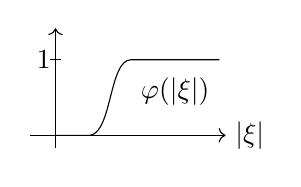
\begin{tikzpicture}[scale=.8]
\draw[->](-.4,0)--(2.7,0)node[right]{$|\xi|$};
\draw[->](0,-.2)--(0,1.7);
\draw(-.08,1.2)--(.08,1.2)node[left]{$1$};
\draw(0,0)--(.55,0)..controls(.9,.05)and(.85,1.2)..(1.2,1.2)--(2.6,1.2);
\node at(1.9,.7){$\varphi(|\xi|)$};
\end{tikzpicture}
\end{adjustbox}
\end{center}
При $s<0$ включ. множитель $\varphi(|\xi|)\sigma(x,\xi)$
(отличие несущ.)
\Unclear{GELFAND-P000125}{cutoff-product}{Перед $\sigma$ густой исправленный знак; справа и снизу формула выделена скобкой.}
\underline{Классич. подход:} $\sigma(x,\xi)$ разлаг. в ряд.
Пусть $s=0$.
\begin{gather*}
\sigma(x,\xi)=\sum a_{mk}(x)Y_{mk}(\xi),\qquad |\xi|=1
\end{gather*}
$|\xi|^mY_{mk}(\xi)$ — гарм. полин. степ. $m$.
\begin{gather*}
Au=\sum a_{mk}(x)F^{-1}Y_{mk}(\xi)Fu\qquad(1)
\end{gather*}
$k=0,1,\ldots,k_m$, $Y_{00}\equiv1$.
\Unclear{GELFAND-P000125}{fourier-cancellation}{Перед «F» зачёркнуты «F Y»-подобные знаки.}
$F$ от сф. ф-й тоже сф. ф-и (они возник.
из предст. гр. вращ.)
\begin{gather*}
m>0,\qquad F^{-1}Y_{mk}(\xi)Fu=\int\frac1{\gamma_m}\frac{Y_{mk}(x-y)}{|x-y|^n}u(y)\,dy\qquad(v.p.)
\end{gather*}
\Unclear{GELFAND-P000125}{kernel-constant}{В знаменателе константа $\gamma_m$ / $\delta_m$.}
\Unclear{GELFAND-P000125}{kernel-cancelled-au}{Перед следующей формулой зачёркнуто «Au».}
\begin{gather*}
Au=v.p.\int K(x,x-y)u(y)\,dy
\end{gather*}
(выкладки формальные)
\underline{3-е опред.}
Рассм. ф-я
\Unclear{GELFAND-P000125}{kernel-variable-cancellation}{Над $K(x,z)$ зачёркнуты «x-y»-подобные знаки.}
$K(x,z)$ полож.-одн. по $z$ ст. $-n$.
\begin{gather*}
\int_{|z|=1}K(x,z)\,dS_z=0.
\end{gather*}

\SourcePage{GELFAND-P000126}{80}
Пусть при $x\to\infty$ стабилиз.
\begin{gather*}
\sigma(x,\xi)=\sigma(\infty,\xi)+\sigma'(x,\xi)
\end{gather*}
$\sigma'$ финитна по $\xi$.
\Unclear{GELFAND-P000126}{finite-variable}{В конце «финитна по» видна $\xi$; чтение $x$ было сравнено и отвергнуто по форме знака. Соседнее условие сформулировано по $x$.}
\begin{gather*}
\sigma(x,D)=\sigma(\infty,D)+\sigma'(x,D)
\end{gather*}
\begin{gather*}
\widetilde{Au}=\sigma(\infty,\xi)\widetilde u+
\frac1{(2\pi)^{n/2}}\int\widetilde\sigma'(\xi-\eta,\eta)\widetilde u(\eta)\,d\eta\qquad(2)
\end{gather*}
\Unclear{GELFAND-P000126}{fourier-left-overwrite}{Знак над/вокруг «Au» и правая его часть обведены и исправлены; чтение преобразования Фурье не вполне ясно.}
Cohn и Nirenberg
$\widetilde\sigma$ пр. Фурье по 1-му перем.
Насколько они эквивал.? Если симв. очень хорошие.
\Unclear{GELFAND-P000126}{equivalence-cancellation}{После «хорошие» зачёркнуто короткое слово.}
В общем случае опр. неэквив. (прив. к разл. кл. опер.)
В каких пр-вах опер. огран.
\begin{gather*}
H^\ell=W_2^{(\ell)},\qquad
\|u\|_\ell^2=\int|\widetilde u|^2(1+|\xi|^2)^\ell\,d\xi
\end{gather*}
\begin{gather*}
\|Au\|_{\ell-s}\quad\text{[зачёркнуто]}\quad\le C\|u\|_\ell
\end{gather*}
\Unclear{GELFAND-P000126}{sobolev-cancellation}{Густо зачёркнут промежуточный член с нормой/индексом $s$}
для гладкой ф-й $\sigma$, разл. в ряд быстро.
\begin{gather*}
\Sigma:|\xi|=1,\qquad\|\sigma(x,\xi)\|_{\Sigma,q}\le const
\quad(\text{не зав. от }x).\qquad(3)
\end{gather*}
Симв. — ф-я от $x$ со знач. в $H_q(\Sigma)$.
\underline{Теорема.}
При $q>\dfrac{n-1}{2}$ и вып. оц. (3), то синг. $\int$ опер. (1)
ограничен в $L_2$. ($\|Au\|_0\le C\|u\|_0$)
\underline{Лемма.}
\begin{gather*}
\|\sigma(x,\xi)\|_q^2\sim\sum m^{2q}|a_{mk}|^2
\end{gather*}
($q=0$ рав-во Парсеваля, $q>0$ св-ва сфер. ф-й)
\underline{Док-во теор.}
\begin{gather*}
S_{\mu\nu}=\sum_{m=\mu}^{\nu}\sum_k a_{mk}(x)A_{mk}u.
\end{gather*}
\begin{gather*}
|S_{\mu\nu}u|^2\le\sum m^{2q}|a_{mk}(x)|^2=\sum m^{-2q}|A_{mk}u|^2
\end{gather*}
\Unclear{GELFAND-P000126}{sum-bound}{Между двумя суммами написано равенство; произведение двух сумм не вставлено.}
\begin{gather*}
\int|S_{\mu\nu}u|^2\,dx\le
\underset{\sup x}{\|\sigma(x,\xi\|_{0,q}^2}
\sum_{m=\mu}^{\nu}m^{-2q}\sum_k\int Y_{mk}^{2}(\xi)\widetilde u(\xi)\,d\xi
\end{gather*}
\Unclear{GELFAND-P000126}{last-integral}{В интеграле $Y_{mk}^{2}(\xi)\widetilde u(\xi)$; квадрат/модуль у $\widetilde u$ не виден. В норме после $\xi$ закрывающая скобка не видна.}
Восп. тожд.
\begin{gather*}
\sum_kY_{mk}^2(\xi)=const\,(k_m+1)
\end{gather*}
(на сф. ф-и с данн. $m$ нетрив. неприв. предст. $\lambda$ В матрице

\SourcePage{GELFAND-P000127}{unlabelled}
одн. строчка из $Y_{mk}(\xi)$ (см. книжку Предст. гр. вращ.)
— а матр. унит.
\begin{gather*}
\int|S_{\mu\nu}u|^2\,dx\le\|\sigma\|_{0,q}^2\cdot\sum m^{2q}k_m\|u\|_0^2.
\end{gather*}
\Unclear{GELFAND-P000127}{top-sum-exponent}{В верхней сумме показатель $2q$ без видимого минуса; ниже используется $-2q$.}
\begin{gather*}
k_m\sim m^{n-2},\qquad -2q+n-2<-1
\end{gather*}
Тогда ряд сойдётся.
$q=\dfrac{n-1}{2}$: уже не будет сход.
По $\xi$ гладк. не нужно.
\Unclear{GELFAND-P000127}{cancelled-second-theorem}{«2-я теор.» зачёркнуто.}
Условия на \underline{$K(x,z)$} в его терминах
\begin{gather*}
K(x,z)=\frac{k(x,z)}{|z|^n}
\end{gather*}
\begin{gather*}
\|k(X,z)\|_q\le const\qquad q> -\frac12\qquad(\text{Норма по }|z|=1)
\end{gather*}
\Unclear{GELFAND-P000127}{kernel-q-sign}{В условии $q> -1/2$ виден короткий минус; значение не заменено по теории.}
\underline{Пример} ($n=2$)
\begin{gather*}
K(z)=\frac{z_1}{(z_1^2+z_2^2)^{3/2}}.
\end{gather*}
\begin{gather*}
\widetilde{Au}(\xi)=\sigma(\infty,\xi)\widetilde u(\xi)+
\frac1{(2\pi)^{n/2}}\int\widetilde\sigma'(\xi-\eta,\eta)\widetilde u(\eta)\,d\eta
\end{gather*}
$\sigma'(x,\xi)$ гладок по $x$ до пор. \underline{$n+1$}.
\begin{gather*}
|\widetilde\sigma'(\xi-\eta,\xi)|\le\frac{const}{(1+|\xi-\eta|^2)^{(n+1)/2}}.
\end{gather*}
\Unclear{GELFAND-P000127}{sigma-argument}{Последний аргумент в оценке исправлен густо: $\xi$ / $\eta$.}
Оцен. свёртка с $\int$ ф-ей. И опр. ограничен в $L_2$.
\begin{gather*}
\left|\int\widetilde\sigma'(\xi-\eta,\eta)\widetilde u(\eta)\,d\eta\right|
\le c\int\left(\frac1{1+|\xi-\eta|^{\text{[неразб.]}}}\right)\widetilde u(\eta)\,d\eta
\end{gather*}
\Unclear{GELFAND-P000127}{convolution-exponent}{$n+1$ / $(n+1)/2$ в густо исправленном показателе.}
1. Ф-ла коммутации.

2. $A\cdot B-\underset{\sigma_1\sigma_2}{A\circ B}$ — меньш. пор.

Отсюда псевдолокальность.
\Unclear{GELFAND-P000127}{final-cancellation}{Перед последней строкой «u»-подобная буква, стрелка вправо и зачёркнутый её конец.}
Обобщ. на мн-зия и эллипт. теория.

\SourcePage{GELFAND-P000128}{81}
\underline{Начнём сначала.}

Синг. $\int$ оператор: (0-го пор.)
\begin{gather*}
(1)\quad\widetilde{Au}(\xi)=F_{x\to\xi}\sigma(x,\xi)u(x)
\end{gather*}
\begin{gather*}
(2)\quad\widetilde{Au}(\xi)=\sigma'(x,\xi)\widetilde u(\xi)+
\end{gather*}
(C. и N.;) (ранние раб.)
\Unclear{GELFAND-P000128}{first-definitions}{В первом определении $\sigma$ без отдельного штриха; во втором $\sigma'$ с отдельным штрихом, и после произведения стоит плюс без дописанного члена.}
\begin{gather*}
(1)\quad\widetilde{Au}(\xi)=\sigma(\infty,\xi)u(\xi)+\int\widetilde\sigma'(\xi-\eta,\xi)\widetilde u(\eta)\,d\eta
\end{gather*}
\begin{gather*}
(2)\quad\widetilde{\mathcal Au}(\xi)=\sigma(\infty,\xi)u(\xi)+\int\widetilde\sigma'(\xi-\eta,\eta)\widetilde u(\eta)\,d\eta
\end{gather*}
\Unclear{GELFAND-P000128}{second-operator}{Второй знак оператора густо исправлен и похож на каллиграфическое $A$ / $B$; над ним волнистая черта.}
Но они отлич. на опер. меньшего пор. ($-1$).
\begin{gather*}
|\widetilde{Au}-\mathcal Au|=\int[\widetilde\sigma'(\xi-\eta,\xi)-\widetilde\sigma'(\xi-\eta,\eta)]\widetilde u(\eta)\,d\eta
\end{gather*}
\begin{gather*}
A^*=\underset{\overline\sigma}{B}\qquad\mathcal A
\end{gather*}
\Unclear{GELFAND-P000128}{adjoint}{После $A^*=$ петлеобразный исправленный знак B; под ним $\overline\sigma$. Справа отдельная A-подобная буква, её связь с равенством неясна.}
(Всё это делается по ф-ле Тейлора)

\underline{Вопр. Гельфанда:}
Можно ли зам. многом. на другие, чтобы получ. та же алгебра.
\Unclear{GELFAND-P000128}{gelfand-question}{Сокращение после «зам.» читается как «многом.» / «многочл.».}
Символ зад. на кокас. пучке.

21/II–66 г. \underline{И. М. Гельфанд.}
(раб. Гельфанда, Граева, Шапиро)

Рассм. $R^n$ или $C^n$. Заданы $\int$ ф-й по $k$-мерн. подпр-вам.
? Как восстановить саму функцию.
(Напр. по прямым в 3-мерн. пр-ве. По всем много,
\Unclear{GELFAND-P000128}{cancelled-parameters}{В начале следующей строки зачёркнуто «6 пар.» / «6-пар.»; далее 4 парам.}
4 парам. Что нужно знать. какие ф-и могут
получиться.
Зная $\int$ по прямым $\Rightarrow\int$ по плоск. $\Rightarrow$ ф-ю $(:)$
Но если 3-парам. сем-во прямых?
Явную ф-лу в общ. виде получить нельзя.
— . —
$R^n$ Рассм. $k$-мерн. подпр-ва с мерой $h$ — в них зад.
понятие объёма. ($k$-мерн. пл. с репером (ед. параллел.))
$H_{n,k}$ — мн-во всех таких $k$-мерн. пл. с объёмом.
Они параллельны, если сущ. сдвиг, перев. одну в другую с
сохр. объёма.

\SourcePage{GELFAND-P000129}{unlabelled}
$G'_{n,k}$ — это мн-во классов эквивалентности по соотн.
параллельности.
\begin{gather*}
f(x)\Rightarrow\varphi(h)=\int_hf(x)\,d\sigma
\end{gather*}
ф-я на $H_{n,k}$.
Условия на $\varphi(h)$ — ?
как по $\varphi(h)$ найти $f(x)$ \Unclear{GELFAND-P000129}{top-extra-sign}{После $f(x)$ густой B-подобный зачёркнутый знак.} наиболее
экономным образом?

\underline{§1. Построение оператора $\mathcal X$.}
\Unclear{GELFAND-P000129}{operator-sign}{Название оператора: каллиграфический X-подобный знак / $\chi$.}
$S_\beta$. $\beta\in R^n$. Рассм. все $k$-мерн.
\Unclear{GELFAND-P000129}{plane-correction}{«подпр.» зачёркнуто; сверху «гиперпл.».}
гиперпл., прох. через $\beta$.
Выделится одна паралл.
\begin{gather*}
S_\beta:G'_{n,k}\longrightarrow H_{n,k}
\end{gather*}
Это глобальное сечение.
рассм. $H_{n,k}\to G'_{n,k}$.
\begin{gather*}
S_\beta^*:\quad\varphi(h)\to\varphi(\alpha,\beta),\qquad\alpha\in G'_{n,k}
\end{gather*}
При фикс. $\beta$ получ. ф-ю на $G'_{n,k}$.
$R^n$ рассм. симм. полилин. форму $B(\xi_1,\ldots,\xi_k)$,
$\xi_i\in R^n$.
По ней строится кососимм. форма
\Unclear{GELFAND-P000129}{alternating-cancellation}{Перед $k^2$ зачёркнуто «из» / короткое слово; сверху вставлено «от».}
от $k^2$ векторов
\begin{gather*}
\Xi=\left\|\begin{matrix}
\xi_{11}&\cdots&\xi_{1k}\\
\xi_{21}&\cdots&\xi_{2k}\\
\vdots&&\vdots\\
\xi_{k1}&\cdots&\xi_{kk}
\end{matrix}\right\|.
\end{gather*}
\begin{gather*}
Det_B(\Xi)=\sum\pm B(\ldots)\text{ —}
\end{gather*}
— число, зав. от элем. \Unclear{GELFAND-P000129}{det-cancellation}{Перед $\Xi$ зачёркнут короткий знак.} $\Xi$.
Для векторов $\xi\in R^1$, $B=\xi_1\cdots\xi_k$ это обычный $\det$.
\Unclear{GELFAND-P000129}{vector-space}{В показателе у R написано 1 / короткий n-подобный знак.}
(лин. со своб. членом — неоднор.)
\underline{Замечание.} Если $B$ опр. в факторпространстве
(в обр. в 0 на $\alpha_0\subset R^n$,
\Unclear{GELFAND-P000129}{quotient-cancellation}{Зачёркнуто «должны бы»-подобное сочетание.}
$B=0$, если хоть бы 1
вект. в $\alpha_0$, то и $Det_B(\Xi)$ тоже фактически опр.
для $\xi_{jk}$ из $R^n/\alpha_0$ (не зав. от выб. предст.)
$\mathcal X\varphi(h)$ будет дифф. формой на $G'_{n,k}$
с коэфф., завис. от $\alpha$.

\SourcePage{GELFAND-P000130}{82}
\begin{gather*}
S_\beta^*\varphi(h)=\varphi(\alpha,\beta)
\end{gather*}
Если зафиксир. \Unclear{GELFAND-P000130}{top-alpha-overwrite}{Густо исправленная буква $\alpha$ / иной знак} $=\alpha_0$ и двигать $\beta$ по $\alpha_0$, то
ничего не изменится. (Зависит не от $\beta$, а не мен., когда
\Unclear{GELFAND-P000130}{beta-parenthesis}{После «а не» сокращение «мен.» / «нем.»; не раскрыто.}
$\beta$ движ. $\parallel\alpha$).
Зафиксир. $\varphi(\alpha_0,\beta)$, рассм. $d_\beta^k\varphi(\alpha_0,\beta)$ —
— симметр. $k$-лин. форма от $k$ дифф. $d\beta$.
Она опред. не от $\beta$, а от фактор. по $\alpha_0$. Опр. в факторпр-ве.
Рассм. $k^2$ вект. $\xi_{ij}$, постр. по этой форме
\begin{gather*}
Det_{d_\beta^k(\varphi(\alpha_0,\beta))}(\Xi)
\end{gather*}
Это зависит от вект. $\xi$ с точн. до векторов $\alpha_0$.
\underline{Теорема.} Постр. по ней кососимм. дифф.
форму в $G'_{n,k}$.
\SourceFigure{GELFAND-P000130}{theorem-line}{Из-под «Теорема.» длинная горизонтальная линия вправо заканчивается двумя вертикальными чертами с несколькими маленькими петлями слева; геометрическое значение не подписано.}
Возьмём в пл. $\alpha_0$ репер, близкие реперы
$e_1,\ldots,e_n$, $e_i'=e_i+\xi_i$.
\Unclear{GELFAND-P000130}{basis-endpoint}{У последнего e индекс похож на $n$; кандидаты $k$ / $nk$ / $n,k$ сравнены, но не подставлены по математике.}
$\xi_i$ — добавки.
(плоск. с точн. до малых высшего порядка)
Они опр. одну и ту же пл. $\Leftrightarrow\xi_i-\widetilde\xi_i\in\alpha_0$.
$k$ близких плоскостей
\begin{gather*}
e'_{ij}=e_i+\xi_{ij}\qquad j=1,\ldots,k
\end{gather*}
Рассм. в качестве $\Xi$ матрицу, опр. $k$ близких плоскостей.
\underline{Теорема 1.}
1. \Unclear{GELFAND-P000130}{theorem-cancellation}{Перед Det зачёркнуто «B»-подобное слово/знак.}
$Det_B(\Xi)$ зав. только от полож.
плоск., а не самой матр.
2. Получ. форма есть $k$-форма (кос.) в $G'_{n,k}$.
\begin{gather*}
\sum\varphi\ldots\quad d\alpha_1\wedge\ldots
\end{gather*}
$d\alpha_i$ — какие-то коорд. в $G$.
Она наз. $\mathcal X\varphi$.
\Unclear{GELFAND-P000130}{coordinate-form}{После $\sum\varphi$ и после $d\alpha_1\wedge$ многоточия; индексы/остальные множители не дописаны. Знак после $d\alpha_1$ похож на $\wedge$ / $\Lambda$.}
\underline{Теорема 2.} Чтобы $\varphi(h)$ была $\int$ от $f(x)$ по $h$ необх.
и дост., чтобы $\mathcal X\varphi$ была замкнутой формой, т. е.
\begin{gather*}
d\mathcal X\varphi\text{ должно }=0
\end{gather*}
(сист. дифф. ур-й —
— ур-я семейства)
\SourcePage{GELFAND-P000131}{unlabelled}
Форма от $\alpha$ и $\beta$: $\psi(\alpha,\beta)\,d\alpha$.
\Unclear{GELFAND-P000131}{form-greek-symbol}{$\psi$ / $\varphi$-подобная буква формы.}
Форма от $R^n\times G'_{n,k}$.
Можно док., что она опред. на $H$ — форма на $H$,
к-рая преобраз. с отобр. $\pi:H_{n,k}\longrightarrow G'_{n,k}$.
Формы на $G'$: $\pi^*$ став. в соотв. форму на $H$.
Рассм. формы из $H$ (получ.),
\Unclear{GELFAND-P000131}{tensor-prefix-cancel}{Перед «тенз. умн.» густо зачёркнут короткий знак.}
тенз. умн. на ф-и в $H$.
Это и есть формы на $H$ с коэфф. $d\alpha$.

\underline{Теор. $3$.} Пусть $\gamma$ — крив.
\Unclear{GELFAND-P000131}{cycle-cancel}{После «крив.» отменены несколько букв/штрихов.}
$k$-мерный цикл в $G'_{n,k}$.
\begin{equation*}\int_\gamma\chi\psi=C_\gamma f'(\beta).\end{equation*}
\Unclear{GELFAND-P000131}{integral-differential-operator}{$\chi$ / $\kappa$ / $x$-подобный знак дифф. оператора.}
\Unclear{GELFAND-P000131}{transformed-f-mark}{У $f$ перед скобкой тонкий штрих: $f'$ / $f$.}
$C_\gamma$ — с точн. до $\pi$ есть индекс пересеч. $\gamma$ с эйлеровским циклом
(все $k$-мерн. подпр-ва, леж. в $(k+1)$-мерном пр-ве).
При нек-рых чётностях не сущ. лок. ф-лы обращения
(
\Unclear{GELFAND-P000131}{radon-parenthetical-cancel}{Зачёркнут фрагмент, похожий на «только $k$-мерн.»}
ср. Радон).
В $C^n$ аналит. ф-ла, но там всегда $C_\gamma\ne0$.
Там всегда сущ. ф-ла обращ.
Надо знать не только $\psi$, но и её производные.

\Unclear{GELFAND-P000131}{delta-prefix-cancel}{Слева зачёркнуто $\delta(h)$-подобное начало и знак равенства.}
\begin{equation*}\int_h f(x)\,d\mu=\delta(h)\cdot f(x).\end{equation*}
[Справа:] в $h$ Ев. мера.
\begin{equation*}C_\gamma f'(\beta)=\int_\gamma\chi\psi(h).\end{equation*}
\begin{equation*}
C_\gamma(\delta(x-\beta),f(x))
=\int_\gamma\chi(\delta(h),f(x)).
\end{equation*}
\begin{equation*}C_\gamma\delta(x-\beta)=\int_\gamma\chi\delta(h).\end{equation*}
\Unclear{GELFAND-P000131}{delta-prime-notation}{У $\delta$ тонкий верхний штрих: $\delta$ / $\delta'$ в формулах.}
[Справа:] $\chi$ — дифф. опер.; $\int$ — по циклу $\gamma$.
В $C^n$ прямые зад. параметрич. ур-ями
$x=\alpha t+\beta$.
\begin{equation*}(\delta(h),f)=\int f(\alpha t+\beta)\,dt\,d\overline t.\end{equation*}

\SourcePage{GELFAND-P000132}{83}
$\chi$ — формы типа $(1,1)$.
\Unclear{GELFAND-P000132}{form-type-first-digit}{Первое число $1$ / $4$-подобный переписанный знак.}
\begin{equation*}
\chi\varphi=\sum_{i=1}^n
\left(\frac{\partial^n}{\partial\beta_i}\,d\alpha_i\cdot
\sum_{i=1}^n\frac{\partial}{\partial\overline\beta_i}\,d\overline\alpha_i\right)\varphi.
\end{equation*}
\Unclear{GELFAND-P000132}{first-partial-overwrite}{У первого $\partial$ повышенный густой $n$-подобный штрих.}
\Unclear{GELFAND-P000132}{form-operator-letters}{$\chi$ / $\kappa$ / $x$-подобный оператор; буква формы $\varphi$ / $\psi$.}
\underline{Оконч. ф-ла:}
\begin{equation*}
C_\gamma\delta(x)=\int_\gamma
\left(\sum\frac{\partial}{\partial\beta_i}\,d\alpha_i\wedge
\sum\frac{\partial}{\partial\overline\beta_i}\,d\overline\alpha_i\right)
\end{equation*}
\Unclear{GELFAND-P000132}{kernel-first-cancel}{Справа отменён $\delta(\ldots)$-подобный фрагмент с густыми скобками.}
[Ниже справа, зачёркнуто:]
$\delta(\alpha_1x\beta_1,\ldots,\alpha_{n-1}x\beta_{n-1})|_{\beta=0}$.
\Unclear{GELFAND-P000132}{kernel-second-cancel}{Знаки между $\alpha_i x$ и $\beta_i$ в отменённой строке неясны.}
[Ниже вставлено:]
\begin{equation*}
\delta(x_1-\alpha_1x_n-\beta_1,\ldots,x_{n-1}-\alpha_{n-1}x_n-\beta_{n-1})\,d
\end{equation*}
\Unclear{GELFAND-P000132}{kernel-trailing-mark}{После вставленного ядра густой $d$- / $x$-подобный знак.}
Прямые зав. от меньшего числа парам., не $2n$.

\underline{Раб. Клейна о волчке.}
(Карпелевич) ($1896$) ($4$ лекции в Принстоне).
Одна точка закрепл.
Вращ. волчка — кривая в группе вращ. $3$-мерн. пр-ва.
Коорд. в этой группе. $2$ способа
(углы Эйлера $\varphi,\theta,\psi$).
Произв. трёх. вращ.,
\Unclear{GELFAND-P000132}{rotation-prefix-cancel}{Перед «вокр. оси» отменён короткий густой знак.}
вокр. оси $Z$, $X$ и $Z$.
Изом. $SO(3)$ и гр. дробно-лин. подст.
$z\longrightarrow\frac{\alpha z+\beta}{\gamma z+\delta}$.
$\begin{pmatrix}\alpha&\beta\\\gamma&\delta\end{pmatrix}$ унит. с опр. $1$ —
\Unclear{GELFAND-P000132}{stereographic-prefix-cancel}{Перед «стереограф. проекция» отменён короткий знак.}
стереограф. проекция.
(Крутим шар — др.-лин. отобр. плоскости.)
(Это $1$-я лекция.)

\underline{$2$-я лекция.}
$\varphi,\psi,\theta$ ищ. как ф-и времени.
$\begin{pmatrix}\alpha&\beta\\\gamma&\delta\end{pmatrix}$
как ф-и времени более простые.
Ур-я движ.:
\begin{equation*}T=\frac12(\varphi'^2+\psi'^2+2\varphi'\psi'\cos\theta+\theta'^2).\end{equation*}
[Справа:] (Все мом. инерции $=1$ отн. точки прикр. — сфера-волчок.)
Потенц. энергия
\Unclear{GELFAND-P000132}{potential-cancel}{Зачёркнуто $\rho$- / $p$-подобное начало.}
$V=p\cos\theta$.
$p$ — расст. до ц. т.
\Unclear{GELFAND-P000132}{potential-distance-letter}{$p$ / $\rho$-подобная буква расстояния.}
$\theta$ — ось $Z$ с ц. т. вертик.
\SourceFigure{GELFAND-P000132}{distance-direction-sketch}{Два луча из общей нижней точки: один почти вертикален, другой наклонён вправо вверх и несёт две густые точки; под наклонным лучом $p$- / $\rho$-подобная метка.}
\begin{equation*}\frac{d}{dt}\frac{\partial T}{\partial\varphi'}=0.\end{equation*}
\begin{equation*}
\begin{cases}
\varphi'+2\psi'\cos\theta=n,\\
\psi'+2\varphi'\cos\theta=e,\\
T+V=h.
\end{cases}
\end{equation*}
\Unclear{GELFAND-P000132}{momentum-cross-coefficients}{В обоих первых интегралах видны коэффициенты $2$ перед смешанным членом.}
Выразим $\varphi',\psi'$ через $\cos\theta=u$ и подст. в то ур-е.
\SourcePage{GELFAND-P000133}{unlabelled}
\begin{equation*}
dt=\frac{du}{\sqrt U},\qquad d\varphi=\frac{n-eu}{1-u^2}\,dt.
\end{equation*}
\Unclear{GELFAND-P000133}{top-angle-letter}{Буква во втором дифференциале: $\varphi$ / $\psi$.}
\begin{equation*}U=2pu^3-2hu^2+2u(\ldots).\end{equation*}
Многочлен $3$-й степени.
$t$ — эллипт. $\int$. Делается его обращение.

\Unclear{GELFAND-P000133}{date-prefix-cancel}{Перед датой короткое зачёркнутое начало.}
\underline{$28/\mathrm{II}$. Продолжение доклада Аграновича.}
\begin{equation*}
Au(x)=\underline{F^{-1}_{\xi\to x}\bigl(F_{x\to\xi}\,\sigma(x,\xi)u(x)\bigr)},\qquad
\sigma(x,t\xi)=t^s\sigma(x,\xi).
\end{equation*}
Это опред. несущ. отлич.
\Unclear{GELFAND-P000133}{negative-order-margin}{На правом поле: «При $s<0$ символ умнож. на ф-ю, вырез. особ. при [зачёркнуто] $\xi=0$».}
\Unclear{GELFAND-P000133}{cancelled-left-equation}{Слева зачёркнута строка, начинающаяся $Au(x)=$; продолжение перекрыто.}
\begin{equation*}\|u\|_{\ell+s}\ge C\|Au\|_\ell.\end{equation*}
\Unclear{GELFAND-P000133}{norm-estimate-overwrite}{Знак сравнения густо исправлен ($\ge$ / $\le$); внутри правой нормы перед $Au$ зачёркнутый знак.}
1) Теорема об огранич.

2) Теорема о композиции.
\begin{equation*}A_1\cdot A_2-A_1\circ A_2=T.\end{equation*}
Под первым произведением: $\sigma_1\sigma_2$; под вторым: $\sigma_1\cdot\sigma_2$.
Справа: пор. $s_1+s_2-1$.

Следствия.

$1^\circ.\quad \varphi(x)A-A\varphi(x)$
\Unclear{GELFAND-P000133}{property-one-short-words}{«с точн. до подч. ком.д. совп.» / «с точн. до подч. кам.д. свя.» — сокращённые слова неуверенно различимы.}
с опер. с символом $\varphi(x)\sigma(x,\xi)$.

$2^\circ.\quad \varphi(x)\cdot\psi(x)=0\ \Rightarrow\ \varphi A(\psi\,\cdot)$ —
опер. на $1$ меньшего порядка.
\Unclear{GELFAND-P000133}{property-two-cancel}{После «Порядка» зачёркнуто короткое слово; далее «(коммутатором — будет $0$)».}

$3^\circ$. Пусть $s=0$. Пусть есть оценка $\|Au\|_1\le c\|u\|_0$
(опер. сглаж.). Тогда символ тожд. $0$ и оператор $0$.

Пусть $\sigma(x,\xi_0)\ne0$. Рассм. символ $\bar\sigma\sigma>0$ в $(x,\xi_0)$.
Сглаж. умн. на огранич. будет сглаж.
\Unclear{GELFAND-P000133}{positive-replacement-words}{«Замен лево-рыми и $\Sigma$» / «Замен неко-рыми и $\Sigma$» — перенос и сокращённое слово сохранены как различимые, чтение неустойчиво.}
Можно добиться $>0$ всюду.
$\sigma(x_0,\xi)>0$ и $\ne0$ уже на меньшем будет сглаж.

3) Теорема о преобр. координат.
$x=x(y)$ — бисм. гладк. невырожд.
\begin{equation*}
\tilde\sigma(y,\eta)=\sigma\left(x(y),\left(\frac{\partial x}{\partial y}\right)^{t-1}\eta\right).
\end{equation*}
\Unclear{GELFAND-P000133}{coordinate-exponent}{Над матрицей видны отдельный апострофоподобный / $t$-подобный штрих и $-1$; чтение $t-1$ / $'^{-1}$ не установлено.}

\SourcePage{GELFAND-P000134}{84}
Закон преобр., как у однородных хар. полиномов
\Unclear{GELFAND-P000134}{cancelled-top-word}{Зачёркнуто «псевдодифф.»; под строкой написано «дифф. опер.».}
Рассм. $\varphi A\psi-\varphi\tilde A\psi=T$ — это подч. опер.

\underline{Авторы.} $s=0$: Calderon, Zygmund, Михлин, Kohn, Nirenberg,
Вишик и Эскин (ряд Фурье по $x$, а коэфф. от $\xi$).
$s>0$ целое — Дынкин. Но исх. опр. — Кальдерон, Зигмунд.
Сили, Кон, Ниренберг — мн-зие без края.
\underline{Сили и Дынкин} — опер. на многообразиях.

Пусть $\underline{s=0}$. $A$ — сингу. $\int$ опер. на мн-зии $V$.
Рассм. $\varphi$ и $\psi$ на $V$.
1) $\operatorname{supp}\varphi\cap\operatorname{supp}\psi=\varnothing
\ \Rightarrow\ \varphi A(\psi u)=Tu$
$(\|Tu\|_1\le c\|u\|_0)$.

2) Пусть $\operatorname{supp}\varphi$ и $\psi$ в коорд. окр.
Тогда
\begin{equation*}\varphi A\psi=\varphi A_\nu\psi+Tu,\end{equation*}
где $A_\nu$ — син. $\int$ опер., запис. в лок. координатах.
Видно, что символ корректно определён как функция на кокасательном пучке.
($A_\nu$ в пересеч.)
Отсюда, в частности, ф-ла преобр. символа.
\SourceFigure{GELFAND-P000134}{overlap-diagram}{Два перекрывающихся округлых контура: слева $x$, справа $y$; в пересечении маленькая петля с густой точкой. Сверху у пересечения $\varphi$, снизу $\psi$; наклонный штрих проходит через пересечение.}
\begin{equation*}
\varphi A\psi=\varphi A_x\psi+T_1=\varphi A_y\psi+T_2.
\end{equation*}
Отсюда $\varphi A_x\psi-\varphi A_y\psi$ сглажив.
Под первым слагаемым вертикальное «$=$» и строка
$\varphi\tilde A_y\psi+$ сглаживающий. Отсюда сглаж. символ.

\begin{equation*}
A=\sum\varphi_\nu A,\qquad
\psi_\nu=\begin{cases}1&\text{в окр. }\operatorname{supp}\varphi_\nu,\\
0&\text{вне окрестн.}\end{cases}
\end{equation*}
\begin{equation*}
A=\sum\varphi_\nu A\psi_\nu+\text{сглаж.}
=\sum\varphi_\nu A_\nu\psi_\nu+\text{сглаж.}
\end{equation*}
\underline{Последнее замечание:}
По символу строится оператор. $\sigma(x,\xi)$ на кокас. пучке,
$\sigma_\nu(x,\xi)$ на $U_\nu$ и разб.
Опер. порядка $\ell$ действ. огранич. из $H_\ell\to H_\ell$.
\Unclear{GELFAND-P000134}{sobolev-order-indices}{Порядок и оба индекса выглядят как $\ell$ / $e$; оба пространства имеют один и тот же видимый индекс.}
\underline{Теор. о композиции:}
\begin{equation*}A\cdot B-A\circ B=T.\end{equation*}
Под $A$: $\sigma_1$; под $B$: $\sigma_2$; под $A\circ B$: $\sigma_1\cdot\sigma_2$.

\SourcePage{GELFAND-P000135}{unlabelled}
\underline{Док-во.}
\begin{align*}
A&=\sum\varphi_k A_k\psi_k+T,\qquad B=\sum\varphi_\ell B_\ell\psi_\ell+T_2,\\
AB&=\sum_{k,\ell}\varphi_k A_k\psi_k\varphi_\ell B_\ell\psi_\ell+\ldots\\
&=\sum_k\sum_\ell\varphi_k\psi_\ell A_\ell\psi_k\varphi_\ell B_\ell\psi_\ell\\
&=\sum_k\sum_\ell\varphi_k\psi_\ell\tilde A_\ell\cdot B_\ell\psi_\ell+\ldots\\
&=\sum_\ell\varphi_\ell A_\ell\circ B_\ell\psi_\ell+\text{сгл.}
\end{align*}
\SourceFigure{GELFAND-P000135}{proof-overlap-diagram}{На верхнем правом поле два перекрывающихся контура, верхний левый с $U_\ell$-образной подписью, нижний правый с $U_k$-образной; пересечение заштриховано косыми штрихами.}
\Unclear{GELFAND-P000135}{proof-first-annotations}{В первой сумме над $\psi_k\varphi_\ell$ дуга с $T^\circ$-образной подписью; снизу разветвлённые стрелки к $\psi_\ell$.}
\Unclear{GELFAND-P000135}{proof-crossed-factors}{Во второй сумме две дуговые стрелки переносят множители влево; в следующей строке над $\psi_\ell\tilde A_\ell$ вставлено $(\varphi_\ell\cdot\psi_k)$ с густо исправленным индексом и знак включения.}
Теор. о композ. доказана.

\underline{Эллиптич. теория.}
$A_s$, $\sigma(P,\xi_P)$; $\xi_P$ — кокас. вектор.
Эллипт. оператор: $\sigma(P,\xi_P)\ne0$ при $\xi_P\ne0$
(если матр., то $\det$).

\underline{Теорема 1.} Эллиптичность эквивалентна нётеровости.
а) Док., что эллипт. опер. нётеровский.
Рассм. $\sigma^{-1}$ тоже символ, однор. степ. $\underline{-s}$,
$\sigma^{-1}\leftrightarrow B$.
\begin{equation*}BA=I_1+T_1,\qquad AB=I_2+T_2.\end{equation*}
\Unclear{GELFAND-P000135}{identity-second-index}{Индекс под вторым $I$ густо переписан, выглядит как $2$.}
Отсюда норм. нётеровость.
$d(A)<\infty,\quad\beta(A)<\infty$.

б) Нёт. $\Rightarrow$ эл. \qquad $s=1$.
\begin{equation*}\|u\|_1\le C(\|Au\|_0+\|u\|_0)\end{equation*}
из нётеровости.
Переход в $R^n$, избав. от завис. симв. от $x$.
Ф-и с мал. носителями и симв. не зав. от $x$.
$\sigma(x_0,\xi_0)=0$ и оц. прив. к противоречию:
$\varphi(x)e^{i\lambda\langle x,\xi_0\rangle}$.

\underline{Теорема 2 (о гладкости).} $Au=f,\quad s=0$.
Пусть $u\in H_0,\ f\in H_1\ \Rightarrow\ u\in H_1$.
\begin{equation*}Au=f,\quad u+T_2f=Bf\in H_1\ \Rightarrow\ u\in H_1.\end{equation*}
\Unclear{GELFAND-P000135}{regularity-source-argument}{В строке написано $u+T_2f=Bf$; после $T_2$ видна $f$-подобная буква.}
Под $T_2f$ стрелка вверх от $H_1$ (сгл.).

\underline{Теорема 3.} Гомотопич. устойчивость индекса
$\chi(A)=d(A)-\beta(A)$.

\SourcePage{GELFAND-P000136}{85}
При малых деформ. символа индекс не меняется.
Непр. деформ. аппрокс. гладкой деформ.
Опер. $A$ с $\sigma\left(x,\frac{\xi}{|\xi|}\right)$ и $B$ с $\sigma_s(x,\xi)$
имеют один и тот же индекс.
\begin{equation*}\underline{B=A\Lambda^s},\qquad\chi(B)=\chi(A)+\chi(\Lambda^s).\end{equation*}
У подчёркнутого равенства на поле: «с точн. до сглаж.».
$\Lambda$ — симв. $\underline{|\xi|}$.
Под $\chi(\Lambda^s)$: «$=0$».
($\Lambda^s$ самосопр. символ — а индекс самосопр. опер. $0$.)

\underline{Теорема об индексе.} (Сили)
$V_n$, $n\times n$ системы.
$\sigma(P,\xi_P)$ — унитарная матрица.
\begin{equation*}S^*(V)\overset{\sigma}{\longrightarrow}U(n)\overset{\rho}{\longrightarrow}S^{2n-1}.\end{equation*}
$S^*(V)$ — кокас. ед. сфера, $2n-1$ разм.
\begin{equation*}
\operatorname{ind}A=\frac{1}{(n-1)!}\operatorname{deg}(\rho\circ\sigma)
\ \Longleftrightarrow\ \operatorname{ind}B=0.
\end{equation*}
Под $B$: $(n-1)\times(n-1)$.
Используется операция $A\#B$ —
$\operatorname{ind}(A\#B)=\operatorname{ind}A\cdot\operatorname{ind}B$.
Для границ областей в $R^{n+1}$ верна такая ф-ла. (прав. часть верна)
Левая ф-ла.

\underline{Подход Хермандера.}
Теор.
\Unclear{GELFAND-P000136}{theorem-cancelled-words}{Два густо зачёркнутых слова перед «о замене».}
о замене. Неудобно, что $C^\infty$-и. символы.
\begin{equation*}
e^{-i\lambda g}A[fe^{ig\lambda}]\sim\sum_0^\infty P_j(f,g)\lambda^{s_j},
\qquad s_j\downarrow-\infty.
\end{equation*}
$f\in C_0^\infty(\Omega),\quad g\in C^\infty(\Omega)$,
веществ., $\operatorname{grad}g\ne0$ на $\operatorname{supp}f$.
\begin{equation*}
\lambda^{-s_N}\left[e^{-i\lambda g}A[fe^{i\lambda g}]
-\sum_0^{N-1}P_j(f,g)\lambda^{s_j}\right]\in
\text{огр. мн-ву в }C^q(\Omega).
\end{equation*}
\Unclear{GELFAND-P000136}{bounded-space-exponent}{Показатель у $C$ петлеобразный с длинным нижним штрихом: $q$ / $\ell$.}
$g\in$ комп. в $C^\infty(\Omega)$ и $A$ должно быть непр.
опер. из $C_0^\infty$ в $C^\infty$.
$\Omega\subset R^n,\quad g=\langle x,\xi\rangle$ — осн.
Рассм. аналог. дифф. опер.

\SourcePage{GELFAND-P000137}{unlabelled}
\underline{Кириллов.} \underline{Борель и Титце.} Редуктивные группы (часть).
\Unclear{GELFAND-P000137}{borel-tits-spelling}{Вторая фамилия выглядит как «Титце» / «Титс».}
\underline{Алгебраические группы.}
Алгебр. мн-зие — лок. афф. схема.
Из кольца $A$ устр. окольцов. пр-во, $\operatorname{Spec}A$ — простые идеалы.
$A=C[x_1,x_2]$. Простой идеал порожд. либо $(x_1-a,x_2-b)$ (точка),
либо неприв. многочленом $I=(P(x_1,x_2))$.
Оно снабж. соот. структурой окольцов. пр-ва.

Алгебр. группа — алгебр. мн-зие, с умнож. $G\times G\to G$,
всюду опр. регул. (рац.) функцией.
\underline{Структ. теорема Шевалле:}
во всякой алг. группе $G$ есть макс. лин. группа $G_0$,
что $G/G_0$ — абелево многообразие.
Лин. группы выделенные из $GL(n,K)$ — алгебр. соотнош.
\Unclear{GELFAND-P000137}{affine-cancelled-word}{После «соотнош.» отдельно густо зачёркнуто слово.}

\underline{Абелево мн-зие} — полное и группа
(полное — «комп.» — напр., проективное) — тогда группа коммутативна.
\underline{Теорема:} всякий гом.
\Unclear{GELFAND-P000137}{abelian-map-abbreviation}{«аб. ф.» / «аб. гр.»}
в лин. и наоборот тривиальны.
Например, алгебраический тор — аб. мн-зие.
\Unclear{GELFAND-P000137}{algebraic-torus-assertion}{Видимая запись: «Например, алгебраический тор — аб. мн-зие».}

Группы $G_a,\ G_m$ — аддит.
\Unclear{GELFAND-P000137}{additive-cancelled-word}{Короткое зачёркнутое слово; сверху вставлено «и мульти.»}
группы поля (алг. группы). Они лин.
\begin{equation*}\begin{pmatrix}1&*\\0&1\end{pmatrix}\qquad(x).\end{equation*}
\underline{Разрешим. группы:} $\exists$ цеп. норм. делителей
\begin{equation*}G_0=G\supset G_1\supset\ldots\supset G_m=\{e\}.\end{equation*}
Что $G_i/G_{i+1}=\begin{cases}G_a,\\G_m.\end{cases}$
\Unclear{GELFAND-P000137}{solvable-parenthesis}{Рядом знак эквивалентности и «(неплно. опр. но разум.)»: первая сокращённая форма неуверенна.}

Радикал — $\max$ связн. (топ. Зариского) норм. делитель.
Над «норм.» вставлено «разрешим.» с дугой и стрелкой.
$R_u(G)$ — длинные черты и кавычки повторения.
\Unclear{GELFAND-P000137}{unipotent-boundary-note}{Под чертами «(унип. радикал)»; затем у нижнего края «из нильпо:: матриц», сокращение и кавычки/двоеточия неустойчивы.}

\SourcePage{GELFAND-P000138}{86}
(Нильпот. $(u-E)^k=0$.)
Редукт. группа — радикал её — тор.
[Над словом «тор»:] $R(G)$.
(Прям. произв. неск. мульт. групп поля.)
\begin{equation*}G\ \text{полупроста}\ \Longleftrightarrow\ R(G)=1.\end{equation*}
$GL(n,K)$ — редукт., $SGL(n,K)$ — полупр.
\underline{Классиф. полупр. групп:} $4$ беск. серии и $5$ особых
(как в группах Ли).
\underline{Осн. понятия — $\max$ тор и система корней.}
\begin{equation*}\begin{pmatrix}a&b\\-b&a\end{pmatrix}\end{equation*}
вещ. матр. — изом. гр. компл. чисел по умн. — тор.
\underline{Все $\max$ торы сопряжены.}
(С тором связ. сист. корней.)

\underline{$21/\mathrm{III}$.}
\Unclear{GELFAND-P000138}{date-under-cancel}{Под датой густая волнистая черта: усиленное подчёркивание / отменённая строка; различимых букв недостаточно.}
\underline{Боровиков.}
\SourceFigure{GELFAND-P000138}{normal-chord-diagram}{Замкнутый округлый контур $L$, точки $M$ внизу слева и $N$ вверху справа, соединённые наклонным отрезком; у концов внутренние почти вертикальные штрихи и дуги углов $\varphi_M$, $\varphi_N$. Подпись: «$L$ с нормалями». Точное положение нормалей и густой нижний участок требуют сверки с оригиналом.}
\underline{Теорема.}
\begin{equation*}\iint\cos\varphi_M\cdot\cos\varphi_N\,dM\,dN=2\pi S.\end{equation*}
($S$ — площадь.)
\Unclear{GELFAND-P000138}{cosine-measure-formula}{Видимая формула содержит $\cos\varphi_M\cdot\cos\varphi_N\,dM\,dN$; знаменатель расстояния не виден.}

\underline{Гельфанд.}
\SourceFigure{GELFAND-P000138}{sphere-section-diagram}{Окружность с внутренней почти горизонтальной эллиптической дугой сечения и меткой $S(x)$ справа. Верхний левый участок сечения густо совпадает с контуром; точное расположение дуг не установлено.}
\begin{equation*}M\left(\int S'^2(x)\,dx\right)=V.\end{equation*}
\Unclear{GELFAND-P000138}{slice-prime-square}{После $S$ вертикальный густой штрих, рядом повышенная $2$: $S'^2$ / $S^2$ с дополнительным штрихом.}
$M$ — универс. пост. (типа $\pi$).

\underline{Лидский. (Виктор Борисович.)}
\begin{equation*}f(z)=\sum_{k=1}^N e^{\alpha_kz}\mathcal P_k(z).\end{equation*}
$\mathcal P_k(z)$ — полин. и асимпт. ряды по $\frac1z$.
\begin{equation*}\sum z_n^{-\sigma}=\zeta(\sigma).\end{equation*}
\Unclear{GELFAND-P000138}{zeta-prefix-cancel}{Перед $\zeta(\sigma)$ густой зачёркнутый знак.}
$\zeta(\sigma)$ всегда целая по $\sigma$.
$z_n$ — нули $f(z)$.
\begin{equation*}\mathcal P_k(z)\simeq p_k(z)+\sum_{s=0}^{\infty}\frac{a_s}{z^s}.\end{equation*}
\Unclear{GELFAND-P000138}{usual-zeta-sin-note}{«Обычная $\zeta$-ф-я — не все $0$ $\sin$ (не от $-\infty$)»: $0$ / $O$ и сжатая связь слов не установлены.}
Док-во — $\int$ Коши.

\underline{Гиндикин.} Обобщение параб. ур-я.
\begin{equation*}\frac{\partial u}{\partial t}+F\left(\frac1i\frac{\partial}{\partial x}\right)u\end{equation*}
\Unclear{GELFAND-P000138}{parabolic-ending-cancel}{После $u$ густо зачёркнуто $=0$-подобное окончание.}
Вместо $\frac{\partial u}{\partial t}$ — любой псевдооператор
$P\left(\frac{\partial}{\partial t}\right)$.
С $P$ связ. сем-во опер., таких, что по $\frac{\partial u}{\partial t}$ получ. параболич.

\SourcePage{GELFAND-P000139}{unlabelled}
Вместо эллипт. — $V$-эллипт., отобр. в конусе, соотв. гиперб. полин.
\underline{Блуждание по прямой} — ур-е теплопроводности.
[В прямоугольной рамке:] \underline{Минлос.}
Модель Изинга.
\SourceFigure{GELFAND-P000139}{ising-lattice}{Небольшая густая прямоугольная решётка, около четырёх клеток по горизонтали и четырёх по вертикали, с утолщёнными пересечениями; отдельные точки или заполненные клетки не различены уверенно.}
$L$ — подмн-во решётки.
\Unclear{GELFAND-P000139}{configuration-parenthesis}{Под записью о $L$: «(только у сущ. точек)» / «(только у сосед. точек)»; сокращение неустойчиво.}
$E(L)$ — число соседей.
\begin{equation*}\Xi=\sum_L e^{-\beta E(L)-\mu N(L)}.\end{equation*}
\Unclear{GELFAND-P000139}{partition-name}{Первый знак суммы — три густых горизонтальных штриха: $\Xi$ / стилизованный $Z$; ниже в логарифме $Z$-подобная буква.}
$N(L)$ — число точек.
\begin{equation*}\lim\frac{\ln Z}{N}=f(\theta,\beta).\end{equation*}
\Unclear{GELFAND-P000139}{limit-first-variable}{Первый аргумент $f$: петлеобразная буква с нижним штрихом, $\theta$ / $\vartheta$ / $\rho$.}
И т. д.
\Unclear{GELFAND-P000139}{final-abbreviated-variables}{Короткая запись после «и т. д.»: «и т. п.» / «и $T$, $\lambda$» / «и $T$, $\rho$»; первый знак после «и» подчёркнут, последний имеет арку и две нисходящие ножки: п-/П-/$\Pi$-/n-подобный, также $\lambda$-/ $\Lambda$-подобный.}








\end{document}
